% **************************************************************************************************************
% A Classic Thesis Style
% Copyright (C) 2018 André Miede and Ivo Pletikosić
% **************************************************************************************************************
%\RequirePackage{silence} % :-\
%    \WarningFilter{scrreprt}{Usage of package `titlesec'}
%    %\WarningFilter{scrreprt}{Activating an ugly workaround}
%    \WarningFilter{titlesec}{Non standard sectioning command detected}
\documentclass[ twoside,openright,titlepage,numbers=noenddot,%1headlines,
                headinclude,footinclude,cleardoublepage=empty,abstract=on,
                BCOR=5mm,paper=a4,fontsize=11pt
                ]{scrreprt}

%********************************************************************
% Note: Make all your adjustments in here
%*******************************************************
% ****************************************************************************************************
% classicthesis-config.tex
% formerly known as loadpackages.sty, classicthesis-ldpkg.sty, and classicthesis-preamble.sty
% Use it at the beginning of your ClassicThesis.tex, or as a LaTeX Preamble
% in your ClassicThesis.{tex,lyx} with % ****************************************************************************************************
% classicthesis-config.tex
% formerly known as loadpackages.sty, classicthesis-ldpkg.sty, and classicthesis-preamble.sty
% Use it at the beginning of your ClassicThesis.tex, or as a LaTeX Preamble
% in your ClassicThesis.{tex,lyx} with % ****************************************************************************************************
% classicthesis-config.tex
% formerly known as loadpackages.sty, classicthesis-ldpkg.sty, and classicthesis-preamble.sty
% Use it at the beginning of your ClassicThesis.tex, or as a LaTeX Preamble
% in your ClassicThesis.{tex,lyx} with \input{classicthesis-config}
% ****************************************************************************************************
% If you like the classicthesis, then I would appreciate a postcard.
% My address can be found in the file ClassicThesis.pdf. A collection
% of the postcards I received so far is available online at
% http://postcards.miede.de
% ****************************************************************************************************


% ****************************************************************************************************
% 0. Set the encoding of your files. UTF-8 is the only sensible encoding nowadays. If you can't read
% äöüßáéçèê∂åëæƒÏ€ then change the encoding setting in your editor, not the line below. If your editor
% does not support utf8 use another editor!
% ****************************************************************************************************
\PassOptionsToPackage{utf8}{inputenc}
  \usepackage{inputenc}

\PassOptionsToPackage{T1}{fontenc} % T2A for cyrillics
  \usepackage{fontenc}


% ****************************************************************************************************
% 1. Configure classicthesis for your needs here, e.g., remove "drafting" below
% in order to deactivate the time-stamp on the pages
% (see ClassicThesis.pdf for more information):
% ****************************************************************************************************
\PassOptionsToPackage{
  drafting=true,    % print version information on the bottom of the pages
  tocaligned=false, % the left column of the toc will be aligned (no indentation)
  dottedtoc=false,  % page numbers in ToC flushed right
  eulerchapternumbers=true, % use AMS Euler for chapter font (otherwise Palatino)
  linedheaders=false,       % chaper headers will have line above and beneath
  floatperchapter=true,     % numbering per chapter for all floats (i.e., Figure 1.1)
  eulermath=false,  % use awesome Euler fonts for mathematical formulae (only with pdfLaTeX)
  beramono=true,    % toggle a nice monospaced font (w/ bold)
  palatino=true,    % deactivate standard font for loading another one, see the last section at the end of this file for suggestions
  style=classicthesis % classicthesis, arsclassica
}{classicthesis}


% ****************************************************************************************************
% 2. Personal data and user ad-hoc commands (insert your own data here)
% ****************************************************************************************************
\newcommand{\myTitle}{Zur Theorie der ordinären Entitäten des Brentanoraumes\xspace}
% \newcommand{\mySubtitle}{Ein topologischer Interpretationsansatz\xspace}
\newcommand{\mySubtitle}{Ein repräsentantenbasierter Interpretationsansatz\xspace}
\newcommand{\myDegree}{Bachelor of science\xspace}
\newcommand{\myName}{Bärbel Hanle\xspace}
\newcommand{\mybirthday}{06.02.1982}
\newcommand{\mybirthtown}{Stuttgart}
\newcommand{\mybirthcountry}{Deutschland}
\newcommand{\myProf}{Dr. Frank Loebe\xspace}
\newcommand{\myOtherProf}{Dr. habil. Ringo Baumann\xspace}
\newcommand{\mySupervisor}{\xspace}
\newcommand{\myFaculty}{Institut für Mathematik und Informatik\xspace}
\newcommand{\myDepartment}{\xspace}
\newcommand{\myUni}{Universität Leipzig\xspace}
\newcommand{\myLocation}{Leipzig\xspace}
\newcommand{\myTime}{10.05.2022\xspace} 
\newcommand{\myVersion}{\classicthesis}

% ********************************************************************
% Setup, finetuning, and useful commands
% ********************************************************************
\providecommand{\mLyX}{L\kern-.1667em\lower.25em\hbox{Y}\kelastrn-.125emX\@}
\newcommand{\ie}{i.\,e.}
\newcommand{\Ie}{I.\,e.}
\newcommand{\eg}{e.\,g.}
\newcommand{\Eg}{E.\,g.}
% ****************************************************************************************************


% ****************************************************************************************************
% 3. Loading some handy packages
% ****************************************************************************************************
% ********************************************************************
% Packages with options that might require adjustments
% ********************************************************************
\PassOptionsToPackage{american,ngerman}{babel} % change this to your language(s), main language last
% Spanish languages need extra options in order to work with this template
%\PassOptionsToPackage{spanish,es-lcroman}{babel}
    \usepackage{babel}

\usepackage{csquotes}
\PassOptionsToPackage{%
  %backend=biber,bibencoding=utf8, %instead of bibtex
  backend=bibtex8,bibencoding=ascii,%
  language=auto,%
  style=authoryear,dashed=false%
  %style=authoryear-comp, % Author 1999, 2010
  %bibstyle=authoryear,dashed=false, % dashed: substitute rep. author with ---
  sorting=nyt, % name, year, title
  maxbibnames=10, % default: 3, et al.
  %backref=true,%
  natbib=true % natbib compatibility mode (\citep and \citet still work)
}{biblatex}
    \usepackage{biblatex}

\PassOptionsToPackage{fleqn}{amsmath}       % math environments and more by the AMS
  \usepackage{amsmath}

% ********************************************************************
% General useful packages
% ********************************************************************
\usepackage{graphicx} %
\usepackage{scrhack} % fix warnings when using KOMA with listings package
\usepackage{xspace} % to get the spacing after macros right

%\usepackage{textcase}
\PassOptionsToPackage{printonlyused,smaller}{acronym}
  \usepackage{acronym} % nice macros for handling all acronyms in the thesis
  %\renewcommand{\bflabel}[1]{{#1}\hfill} % fix the list of acronyms --> no longer working
  %\renewcommand*{\acsfont}[1]{\textsc{#1}}
  %\renewcommand*{\aclabelfont}[1]{\acsfont{#1}}
  %\def\bflabel#1{{#1\hfill}}
  \def\bflabel#1{{\acsfont{#1}\hfill}}
  \def\aclabelfont#1{\acsfont{#1}}
  
  %\renewcommand{\acsfont}[1]{{\scshape \MakeTextLowercase{#1}}}
  
\PassOptionsToPackage{activate={true,nocompatibility},final,tracking=true,kerning=true,spacing=true,factor=1100,stretch=10,shrink=10,final}{microtype}%final-even in draft mode
\usepackage[]{microtype}
% ****************************************************************************************************
%\usepackage{pgfplots} % External TikZ/PGF support (thanks to Andreas Nautsch)
%\usetikzlibrary{external}
%\tikzexternalize[mode=list and make, prefix=ext-tikz/]
% ****************************************************************************************************

% ****************************************************************************************************
% 4. Setup floats: tables, (sub)figures, and captions
% ****************************************************************************************************
\usepackage{tabularx} % better tables
  \setlength{\extrarowheight}{3pt} % increase table row height
\newcommand{\tableheadline}[1]{\multicolumn{1}{l}{\spacedlowsmallcaps{#1}}}
\newcommand{\myfloatalign}{\centering} % to be used with each float for alignment
\usepackage{subfig}
% ****************************************************************************************************


% ****************************************************************************************************
% 5. Setup code listings
% ****************************************************************************************************
\usepackage{listings}
%\lstset{emph={trueIndex,root},emphstyle=\color{BlueViolet}}%\underbar} % for special keywords
\lstset{language=[LaTeX]Tex,%C++,
  morekeywords={PassOptionsToPackage,selectlanguage},
  keywordstyle=\color{RoyalBlue},%\bfseries,
  basicstyle=\small\ttfamily,
  %identifierstyle=\color{NavyBlue},
  commentstyle=\color{Green}\ttfamily,
  stringstyle=\rmfamily,
  numbers=none,%left,%
  numberstyle=\scriptsize,%\tiny
  stepnumber=5,
  numbersep=8pt,
  showstringspaces=false,
  breaklines=true,
  %frameround=ftff,
  %frame=single,
  belowcaptionskip=.75\baselineskip
  %frame=L
}
% ****************************************************************************************************




% ****************************************************************************************************
% 6. Last calls before the bar closes
% ****************************************************************************************************
% ********************************************************************
% Her Majesty herself
% ********************************************************************
\usepackage[dottedtoc]{classicthesis}


% ********************************************************************
% Fine-tune hyperreferences (hyperref should be called last)
% ********************************************************************
\hypersetup{%
  %draft, % hyperref's draft mode, for printing see below
  colorlinks=true, linktocpage=true, pdfstartpage=3, pdfstartview=FitV,%
  % uncomment the following line if you want to have black links (e.g., for printing)
  %colorlinks=false, linktocpage=false, pdfstartpage=3, pdfstartview=FitV, pdfborder={0 0 0},%
  breaklinks=true, pageanchor=true,%
  pdfpagemode=UseNone, %
  % pdfpagemode=UseOutlines,%
  plainpages=false, bookmarksnumbered, bookmarksopen=true, bookmarksopenlevel=1,%
  hypertexnames=true, pdfhighlight=/O,%nesting=true,%frenchlinks,%
  urlcolor=CTurl, linkcolor=CTlink, citecolor=CTcitation, %pagecolor=RoyalBlue,%
  %urlcolor=Black, linkcolor=Black, citecolor=Black, %pagecolor=Black,%
  pdftitle={\myTitle},%
  pdfauthor={\textcopyright\ \myName, \myUni, \myFaculty},%
  pdfsubject={},%
  pdfkeywords={},%
  pdfcreator={pdfLaTeX},%
  pdfproducer={LaTeX with hyperref and classicthesis}%
}

%**************************************************************************
% Eigene Pakete
%**************************************************************************
\usepackage{amssymb} % für \varnothing
\usepackage{stmaryrd} % Widerspruchsblitz
\usepackage{amsthm} % Für Theoremumgebungen
  \usepackage{zref-perpage} % FL: zref-perpage is there for 
    % fixing a MikTeX problem with zref, which is loaded by mdframed;
	  % cf. https://github.com/ho-tex/zref/issues/14
\usepackage[framemethod=tikz]{mdframed} % Rand für Theoreme
\usepackage{multirow}
\usepackage{makecell} % Zeilenumburuch innerhalb einer Zelle
\usepackage{longtable} % Tabelle über mehrere Seiten´
\usepackage{subcaption}
% \usepackage[labelformat=parens,labelsep=quad,skip=3pt]{caption}
%\usepackage{graphicx}

%\usepackage{textcase}



% ********************************************************************
% Setup autoreferences (hyperref and babel)
% ********************************************************************
% There are some issues regarding autorefnames
% http://www.tex.ac.uk/cgi-bin/texfaq2html?label=latexwords
% you have to redefine the macros for the
% language you use, e.g., american, ngerman
% (as chosen when loading babel/AtBeginDocument)
% ********************************************************************
\makeatletter
\@ifpackageloaded{babel}%
  {%
    \addto\extrasamerican{%
		  \renewcommand*{\figurename}{Fig.}%
      \renewcommand*{\figureautorefname}{Figure}%
      \renewcommand*{\tableautorefname}{Table}%
      \renewcommand*{\partautorefname}{Part}%
      \renewcommand*{\chapterautorefname}{Chapter}%
      \renewcommand*{\sectionautorefname}{Section}%
      \renewcommand*{\subsectionautorefname}{Section}%
      \renewcommand*{\subsubsectionautorefname}{Section}%
    }%
    \addto\extrasngerman{%
		  \renewcommand*{\figurename}{Abb.}%
      \renewcommand*{\paragraphautorefname}{Absatz}%
      \renewcommand*{\subparagraphautorefname}{Unterabsatz}%
      \renewcommand*{\footnoteautorefname}{Fu\"snote}%
      \renewcommand*{\FancyVerbLineautorefname}{Zeile}%
      \renewcommand*{\theoremautorefname}{Theorem}%
      \renewcommand*{\appendixautorefname}{Anhang}%
      \renewcommand*{\equationautorefname}{Gleichung}%
      \renewcommand*{\itemautorefname}{Punkt}%
    }%
      % Fix to getting autorefs for subfigures right (thanks to Belinda Vogt for changing the definition)
      \providecommand{\subfigureautorefname}{\figureautorefname}%
    }{\relax}
\makeatother


% ********************************************************************
% Development Stuff
% ********************************************************************
\listfiles
%\PassOptionsToPackage{l2tabu,orthodox,abort}{nag}
%  \usepackage{nag}
%\PassOptionsToPackage{warning, all}{onlyamsmath}
%  \usepackage{onlyamsmath}


% ****************************************************************************************************
% 7. Further adjustments (experimental)
% ****************************************************************************************************
% ********************************************************************
% Changing the text area
% ********************************************************************
%\areaset[current]{312pt}{761pt} % 686 (factor 2.2) + 33 head + 42 head \the\footskip
%\setlength{\marginparwidth}{7em}%
%\setlength{\marginparsep}{2em}%

% ********************************************************************
% Using different fonts
% ********************************************************************
%\usepackage[oldstylenums]{kpfonts} % oldstyle notextcomp
% \usepackage[osf]{libertine}
%\usepackage[light,condensed,math]{iwona}
%\renewcommand{\sfdefault}{iwona}
%\usepackage{lmodern} % <-- no osf support :-(
%\usepackage{cfr-lm} %
%\usepackage[urw-garamond]{mathdesign} <-- no osf support :-(
%\usepackage[default,osfigures]{opensans} % scale=0.95
%\usepackage[sfdefault]{FiraSans}
% \usepackage[opticals,mathlf]{MinionPro} % onlytext
% ********************************************************************
%\usepackage[largesc,osf]{newpxtext}
%\linespread{1.05} % a bit more for Palatino
% Used to fix these:
% https://bitbucket.org/amiede/classicthesis/issues/139/italics-in-pallatino-capitals-chapter
% https://bitbucket.org/amiede/classicthesis/issues/45/problema-testatine-su-classicthesis-style
% ********************************************************************
% ****************************************************************************************************

% ****** Custom
%\usepackage[disable]{todonotes}
\usepackage{todonotes}
\usepackage{cleveref}

%***************************************************************************
% Umgebungen
%***************************************************************************
\theoremstyle{definition}

\newtheorem{dfn}{Def}[section]
\newtheorem{nota}[dfn]{Notation}
\newtheorem{konv}[dfn]{Konvention}

\newtheorem{satz}[dfn]{Satz}
\newtheorem{kor}[dfn]{Kor}
\newtheorem{hyp}[dfn]{Hyp}

\newtheorem{bsp}[dfn]{Bsp}
\newtheorem{gegenbsp}[dfn]{Gegenbeispiel}
\newtheorem{bem}[dfn]{Bem}
\newtheorem*{erin}{Erinnerung}
\newtheorem*{bew}{Bew}
\newtheorem*{bewidee}{Beweisidee}

\mdfdefinestyle{grey}{
    skipabove=5pt,
    skipbelow=5pt,
    innerbottommargin=12pt,
    %innerleftmargin=20pt
    innerrightmargin=20pt
    leftmargin=5pt,
    rightmargin=5pt,
    %linewidth=0.2pt,
    roundcorner=2pt,
    backgroundcolor=black!5,
    hidealllines=true,
    needspace=60pt,
		aftersingleframe={\noindent},
}

\mdfdefinestyle{white}{
    skipabove=5pt,
    skipbelow=5pt,
    innerbottommargin=12pt,
    %innerleftmargin=20pt
    innerrightmargin=20pt
    leftmargin=5pt,
    rightmargin=5pt,
    %linewidth=0.2pt,
    roundcorner=2pt,
    %backgroundcolor=black!5,
    %hidealllines=true
}

\mdfdefinestyle{beweis}{
    skipabove=0pt,
    skipbelow=5pt,
    innerbottommargin=12pt,
    %innerleftmargin=20pt
    innerrightmargin=20pt
    leftmargin=5pt,
    rightmargin=5pt,
    %linewidth=0.2pt,
    roundcorner=2pt,
    %backgroundcolor=black!5,
    %hidealllines=true
    linecolor=black!10
%     rightline=false
%     bottomline=false
%     topline=false
}

\surroundwithmdframed[style=grey]{dfn}
\surroundwithmdframed[style=grey]{nota}
\surroundwithmdframed[style=grey]{konv}
\surroundwithmdframed[style=grey]{satz}
\surroundwithmdframed[style=grey]{kor}
\surroundwithmdframed[style=grey]{hyp}
\surroundwithmdframed[style=white]{bsp}
\surroundwithmdframed[style=white]{gegenbsp}
\surroundwithmdframed[style=white]{bem}
\surroundwithmdframed[style=white]{erin}
\surroundwithmdframed[style=beweis]{bew}
\surroundwithmdframed[style=beweis]{bewidee}




\DeclareRobustCommand{\BSO}{\mathcal{BS^O}}

%--------------------------------------------

\newcommand{\thmemph}{\textbf}
\newcommand{\textemph}{\spacedlowsmallcaps}
%\renewcommand{\marginpar}[2][]{} % marginpars verstecken



%*****************************************************************************
% BS-Kommandos
%********************************************************************************
% 
% %%%%%%%%%%%%%%%%%%%%%%%%%%%%%%%%%%%%%%%%%%%%%%%%%%%%%%%%
% % OPTION uniformSymbols STARTS
% %%%%%%%%%%%%%%%%%%%%%%%%%%%%%%%%%%%%%%%%%%%%%%%%%%%%%%%%%%
% \DeclareOption{uniformSymbols}{%
% %
% \newcommand{\GSymbolFont}[1]{#1}
% %
% } %OPTION uniformSymbols ENDS HERE
% %%%%%%%%%%%%%%%%%%%%%%%%%%%%%%%%%%%%%%%%%%%%%%%%%%%
% %%%%%%%%%%%%%%%%%%%%%%%%%%%%%%%%%%%%%%%%%%%%%%%%%%% 
% 
% %%%%%%%%%%%%%%%%%%%%%%%%%%%%%%%%%%%%%%%%%%%%%%%%%%%%%%%%
% % OPTION mboxSymbols STARTS
% %%%%%%%%%%%%%%%%%%%%%%%%%%%%%%%%%%%%%%%%%%%%%%%%%%%%%%%%%%
% \DeclareOption{mboxSymbols}{%
% %
% \renewcommand{\GSymbolFont}[1]{\mbox{#1}}
% %
% } %OPTION mboxSymbols ENDS HERE
% %%%%%%%%%%%%%%%%%%%%%%%%%%%%%%%%%%%%%%%%%%%%%%%%%%%
% %%%%%%%%%%%%%%%%%%%%%%%%%%%%%%%%%%%%%%%%%%%%%%%%%%% 
% 
% %%%%%%%%%%%%%%%%%%%%%%%%%%%%%%%%%%%%%%%%%%%%%%%%%%%%%%%%
% % OPTION mboxSymbols STARTS
% %%%%%%%%%%%%%%%%%%%%%%%%%%%%%%%%%%%%%%%%%%%%%%%%%%%%%%%%%%
% \DeclareOption{italicSymbols}{%
% %
% \renewcommand{\GSymbolFont}[1]{\ensuremath{\mathit{#1}}}
% %
% } %OPTION mboxSymbols ENDS HERE
% %%%%%%%%%%%%%%%%%%%%%%%%%%%%%%%%%%%%%%%%%%%%%%%%%%%
% %%%%%%%%%%%%%%%%%%%%%%%%%%%%%%%%%%%%%%%%%%%%%%%%%%% 
% 
% % Execution of options
% \ExecuteOptions{manAxiomStyle,uniformSymbols}

\newcommand{\GSymbolFont}[1]{\ensuremath{\mathit{#1}}}
\newcommand{\AuxD}{D\hspace*{-0.25ex}}


\newcommand{\GC}{\ensuremath{\GSymbolFont{C}}}
\newcommand{\GCrossdDBn}{\ensuremath{\GSymbolFont{Cross\Gd DB_{n}}}}
\newcommand{\GCrossoneDBn}{\ensuremath{\GSymbolFont{Cross1DB_{n}}}}
\newcommand{\GCrosstwoDBn}{\ensuremath{\GSymbolFont{Cross2DB_{n}}}}
\newcommand{\GCrosszeroDBn}{\ensuremath{\GSymbolFont{Cross0DB_{n}}}}
\newcommand{\Gc}{\ensuremath{\GSymbolFont{c}}}
\newcommand{\Gcrossonedbn}{\ensuremath{\GSymbolFont{cross1db_{n}}}}
\newcommand{\Gcrosstwodbn}{\ensuremath{\GSymbolFont{cross2db_{n}}}}
%\newcommand{\Gcrosszerodb}{\ensuremath{\GSymbolFont{cross0db}}}
\newcommand{\Gcrosszerodbn}{\ensuremath{\GSymbolFont{cross0db_{n}}}}

\newcommand{\Gd}{\boldsymbol{\mathsf{d}}}
\newcommand{\Gone}{\boldsymbol{\mathsf{1}}}
\newcommand{\Gtwo}{\boldsymbol{\mathsf{2}}}
\newcommand{\Gthree}{\boldsymbol{\mathsf{3}}}
\newcommand{\GdD}{\ensuremath{\GSymbolFont{\Gd D}}}
\newcommand{\GdDB}{\ensuremath{\GSymbolFont{\Gd\AuxD B}}}
\newcommand{\GdDC}{\ensuremath{\GSymbolFont{\Gd\AuxD C}}}
\newcommand{\GdDE}{\ensuremath{\GSymbolFont{\Gd\AuxD E}}}
\newcommand{\Gddb}{\ensuremath{\GSymbolFont{\Gd db}}}
\newcommand{\Gddhypp}{\ensuremath{\GSymbolFont{\Gd dhypp}}}
\newcommand{\Gdmdhypp}{\ensuremath{\GSymbolFont{\Gdm dhypp}}}
\newcommand{\Gdircomp}{\ensuremath{\GSymbolFont{dircomp}}}
\newcommand{\Gddircomp}{\ensuremath{\GSymbolFont{\Gd dircomp}}}
\newcommand{\dircomp}{\ensuremath{\GSymbolFont{\Gdp dircomp}}}
\newcommand{\Gdp}{\boldsymbol{\mathsf{(d+1)}}}
\newcommand{\Gdm}{\boldsymbol{\mathsf{(d-1)}}}

\newcommand{\GExOrd}{\ensuremath{\GSymbolFont{ExOrd}}}
\newcommand{\Gequ}{\ensuremath{\GSymbolFont{equ}}}
\newcommand{\Geqdim}{\ensuremath{\GSymbolFont{eqdim}}}
\newcommand{\Gexc}{\ensuremath{\GSymbolFont{exc}}}

\newcommand{\GGrSB}{\ensuremath{\GSymbolFont{Gr\hspace*{-0.25ex}SB}}}
\newcommand{\Ggrsb}{\ensuremath{\GSymbolFont{gr\hspace*{-0.25ex}sb}}}

\newcommand{\Ghypp}{\ensuremath{\GSymbolFont{hypp}}}

\newcommand{\GiCCDd}{\ensuremath{\GSymbolFont{i}_{\Gd}\GSymbolFont{CC}}}
\newcommand{\GiCCDone}{\ensuremath{\GSymbolFont{i}_{1}\GSymbolFont{CC}}}
\newcommand{\GiCCDtwo}{\ensuremath{\GSymbolFont{i}_{2}\GSymbolFont{CC}}}
\newcommand{\GiCCDzero}{\ensuremath{\GSymbolFont{i}_{0}\GSymbolFont{CC}}}
\newcommand{\Ginpart}{\ensuremath{\GSymbolFont{inpart}}}
\newcommand{\Gintersect}{\ensuremath{\GSymbolFont{intsect}}}
\newcommand{\Gintersectn}{\ensuremath{\GSymbolFont{intsect_{n}}}}

\newcommand{\GLDE}{\ensuremath{\GSymbolFont{LDE}}}

\newcommand{\Gcont}{\ensuremath{\GSymbolFont{cont}}}
\newcommand{\Gstrictsb}{\ensuremath{\GSymbolFont{strictsb}}}
\newcommand{\Gweaksb}{\ensuremath{\GSymbolFont{weaksb}}}

%\newcommand{\GkCCDd}{\ensuremath{\GSymbolFont{k}_{\Gd}\GSymbolFont{CC}}}
%\newcommand{\GkCCDone}{\ensuremath{\GSymbolFont{k}_{1}\GSymbolFont{CC}}}
%\newcommand{\GkCCDtwo}{\ensuremath{\GSymbolFont{k}_{2}\GSymbolFont{CC}}}
\newcommand{\GkCCDzero}{\ensuremath{\GSymbolFont{k}_{0}\GSymbolFont{CC}}}

%\newcommand{\GlCCDd}{\ensuremath{\GSymbolFont{l}_{\Gd}\GSymbolFont{CC}}}
\newcommand{\GlCCDone}{\ensuremath{\GSymbolFont{l}_{1}\GSymbolFont{CC}}}
%\newcommand{\GlCCDtwo}{\ensuremath{\GSymbolFont{l}_{2}\GSymbolFont{CC}}}
%\newcommand{\GlCCDzero}{\ensuremath{\GSymbolFont{l}_{0}\GSymbolFont{CC}}}

\newcommand{\GnCCDd}{\ensuremath{\GSymbolFont{n}_{\Gd}\GSymbolFont{CC}}}
\newcommand{\GnCCDone}{\ensuremath{\GSymbolFont{n}_{1}\GSymbolFont{CC}}}
\newcommand{\GnCCDtwo}{\ensuremath{\GSymbolFont{n}_{2}\GSymbolFont{CC}}}
\newcommand{\GnCCDzero}{\ensuremath{\GSymbolFont{n}_{0}\GSymbolFont{CC}}}
%\newcommand{\GnminusiCCDd}{\ensuremath{\GSymbolFont{(n-i)}_{\Gd}\GSymbolFont{CC}}}
\newcommand{\GnminusiCCDone}{\ensuremath{\GSymbolFont{(n-i)}_{1}\GSymbolFont{CC}}}
%\newcommand{\GnminusiCCDtwo}{\ensuremath{\GSymbolFont{(n-i)}_{2}\GSymbolFont{CC}}}
\newcommand{\GnminusiCCDzero}{\ensuremath{\GSymbolFont{(n-i)}_{0}\GSymbolFont{CC}}}


\newcommand{\GOrd}{\ensuremath{\GSymbolFont{Ord}}}
\newcommand{\GoneCCDd}{\ensuremath{\GSymbolFont{1}_{\Gd}\GSymbolFont{CC}}}
\newcommand{\GoneCCDone}{\ensuremath{\GSymbolFont{1}_{1}\GSymbolFont{CC}}}
\newcommand{\GoneCCDtwo}{\ensuremath{\GSymbolFont{1}_{2}\GSymbolFont{CC}}}
\newcommand{\GoneCCDzero}{\ensuremath{\GSymbolFont{1}_{0}\GSymbolFont{CC}}}
\newcommand{\GoneD}{\ensuremath{\GSymbolFont{1D}}}
\newcommand{\GoneDB}{\ensuremath{\GSymbolFont{1\AuxD B}}}
\newcommand{\GoneDC}{\ensuremath{\GSymbolFont{1DC}}}
\newcommand{\GoneDE}{\ensuremath{\GSymbolFont{1\AuxD E}}}
\newcommand{\Gonedb}{\ensuremath{\GSymbolFont{1db}}}
\newcommand{\Gonecont}{\ensuremath{\GSymbolFont{1cont}}}
\newcommand{\Gonedircomp}{\ensuremath{\GSymbolFont{1dircomp}}}
\newcommand{\Gonedhypp}{\ensuremath{\GSymbolFont{1dhypp}}}

\newcommand{\Gpartition}{\ensuremath{\GSymbolFont{partition}}}
\newcommand{\Gpartitioni}{\ensuremath{\GSymbolFont{partition_{i}}}}
\newcommand{\Gpartitionn}{\ensuremath{\GSymbolFont{partition_{n}}}}

\newcommand{\GReg}{\ensuremath{\GSymbolFont{SReg}}}
\newcommand{\Grelcompl}{\ensuremath{\GSymbolFont{rcompl}}}
\newcommand{\Grelcompln}{\ensuremath{\GSymbolFont{rcompl_{n}}}}

\newcommand{\GSB}{\ensuremath{\GSymbolFont{S\hspace*{-0.25ex}B}}}
\newcommand{\GSReg}{\ensuremath{\GSymbolFont{S\hspace*{-0.25ex}Reg}}}
\newcommand{\Gsb}{\ensuremath{\GSymbolFont{sb}}}
\newcommand{\Gscoinc}{\ensuremath{\GSymbolFont{scoinc}}}
\newcommand{\Gsov}{\ensuremath{\GSymbolFont{sov}}}
\newcommand{\Gspart}{\ensuremath{\GSymbolFont{spart}}}
\newcommand{\Gsppart}{\ensuremath{\GSymbolFont{sppart}}}
\newcommand{\Gsum}{\ensuremath{\GSymbolFont{sum}}}
\newcommand{\Gsumi}{\ensuremath{\GSymbolFont{sum_{i}}}}
\newcommand{\Gsumn}{\ensuremath{\GSymbolFont{sum_{n}}}}

\newcommand{\GTop}{\ensuremath{\GSymbolFont{Top}}}
\newcommand{\Gtangpart}{\ensuremath{\GSymbolFont{tangpart}}}
\newcommand{\GtwoD}{\ensuremath{\GSymbolFont{2D}}}
\newcommand{\GtwoDB}{\ensuremath{\GSymbolFont{2\AuxD B}}}
\newcommand{\GtwoDC}{\ensuremath{\GSymbolFont{2DC}}}
\newcommand{\GtwoDE}{\ensuremath{\GSymbolFont{2\AuxD E}}}
\newcommand{\Gtwodb}{\ensuremath{\GSymbolFont{2db}}}
\newcommand{\Gtwodhypp}{\ensuremath{\GSymbolFont{2dhypp}}}

\newcommand{\GzeroD}{\ensuremath{\GSymbolFont{0D}}}
\newcommand{\GzeroDB}{\ensuremath{\GSymbolFont{0\AuxD B}}}
\newcommand{\GzeroDC}{\ensuremath{\GSymbolFont{0DC}}}
\newcommand{\GzeroDE}{\ensuremath{\GSymbolFont{0\AuxD E}}}
\newcommand{\Gzerocont}{\ensuremath{\GSymbolFont{0cont}}}
\newcommand{\Gzerodb}{\ensuremath{\GSymbolFont{0db}}}
\newcommand{\Gzerodhypp}{\ensuremath{\GSymbolFont{0dhypp}}}



%MISC
\newcommand{\bs}{\backslash}
\newcommand{\gap}{\\[0.1ex]\mbox{}}
\newcommand{\m}[1]{\ensuremath{\mathcal{#1}}}
%\newcommand{\MS}{\ensuremath{\mathrel{.}}}
\newcommand{\MS}{\ensuremath{\,.\,}}
\newcommand{\theoryBS}{\ensuremath{\mathcal{BS}}\xspace}
\newcommand{\theoryBSone}{\ensuremath{\mathcal{BS}_{\text{v}1}}\xspace}
\newcommand{\theoryBT}{\ensuremath{\mathcal{BT}}}
\newcommand{\theoryBTC}{\ensuremath{\mathcal{BT}^{\mathcal{C}}}}
\newcommand{\theoryBTR}{\ensuremath{\mathcal{BT}^{\mathcal{R}}}}
\newcommand{\trel}[1]{\textit{#1}}

%********************************************************
% Eigene Kommandos
%********************************************************

\newcommand{\theoryBSO}{\ensuremath{\mathcal{BS}^{\mathcal{O}}}}
%\newcommand{\strukt}{\ensuremath{{\mathcal{R}\text{-Struktur}}}}
\newcommand{\strukt}{$\mathcal{R}$-Struktur\xspace}
\newcommand{\rep}{\ensuremath{\mathcal{R}}}
\newcommand{\univ}{\ensuremath{\mathcal{U}}}
\newcommand{\R}{\ensuremath{\mathbb{R}}}
\newcommand{\N}{\ensuremath{\mathbb{N}}}

\newcommand{\offen}{\ensuremath{\mathcal{O}}}
\newcommand{\abg}{\ensuremath{\mathcal{C}}}
\newcommand{\einf}{\ensuremath{\mathcal{S}}}
\newcommand{\CO}{\ensuremath{\mathcal{CO}}}
\newcommand{\OC}{\ensuremath{\mathcal{OC}}}

\newcommand{\cl}{\ensuremath{\text{cl}}}
\newcommand{\op}{\ensuremath{\text{op}}}
\newcommand{\co}{\ensuremath{\text{co}}}
\newcommand{\oc}{\ensuremath{\text{oc}}}
\newcommand{\HP}{\ensuremath{\text{HP}}}
\newcommand{\rand}{\ensuremath{\partial}}
\newcommand{\ball}{\ensuremath{B}}

\newcommand{\Gdim}{\ensuremath{\text{dim}}}
\newcommand{\Gmaxcon}{\ensuremath{\GSymbolFont{maxcon}}}
\newcommand{\Gloczerodc}{\ensuremath{\GSymbolFont{loc0dc}}}
\newcommand{\Gloconedc}{\ensuremath{\GSymbolFont{loc1dc}}}

\newcommand{\deshalb}{\ensuremath{\rightarrow}}

%***************************************************************
% Struktursymbole
%***************************************************************

\newcommand{\SdDB}{\ensuremath{\GSymbolFont{\Gd\AuxD B}^\mathcal{O}}}
\newcommand{\SdDC}{\ensuremath{\GSymbolFont{\Gd\AuxD C}^\mathcal{O}}}
\newcommand{\SdDE}{\ensuremath{\GSymbolFont{\Gd\AuxD E}^\mathcal{O}}}
\newcommand{\Sddb}{\ensuremath{\GSymbolFont{\Gd db}^\mathcal{O}}}
\newcommand{\Sddhypp}{\ensuremath{\GSymbolFont{\Gd dhypp}^\mathcal{O}}}
\newcommand{\Sdmdhypp}{\ensuremath{\GSymbolFont{\Gdm dhypp}^\mathcal{O}}}
\newcommand{\Sdircomp}{\ensuremath{\GSymbolFont{dircomp}^\mathcal{O}}}
\newcommand{\Sddircomp}{\ensuremath{\GSymbolFont{\Gd dircomp}^\mathcal{O}}}

\newcommand{\SExOrd}{\ensuremath{\GSymbolFont{ExOrd}^\mathcal{O}}}
\newcommand{\Sequ}{\ensuremath{\GSymbolFont{equ}^\mathcal{O}}}
\newcommand{\Seqdim}{\ensuremath{\GSymbolFont{eqdim}^\mathcal{O}}}
\newcommand{\Sexc}{\ensuremath{\GSymbolFont{exc}^\mathcal{O}}}

\newcommand{\SGrSB}{\ensuremath{\GSymbolFont{Gr\hspace*{-0.25ex}SB}^\mathcal{O}}}
\newcommand{\Sgrsb}{\ensuremath{\GSymbolFont{gr\hspace*{-0.25ex}sb}^\mathcal{O}}}

\newcommand{\Shypp}{\ensuremath{\GSymbolFont{hypp}^\mathcal{O}}}

\newcommand{\SiCCDd}{\ensuremath{\GSymbolFont{i}_{\Gd}\GSymbolFont{CC}^\mathcal{O}}}
\newcommand{\SiCCDone}{\ensuremath{\GSymbolFont{i}_{1}\GSymbolFont{CC}^\mathcal{O}}}
\newcommand{\SiCCDtwo}{\ensuremath{\GSymbolFont{i}_{2}\GSymbolFont{CC}^\mathcal{O}}}
\newcommand{\SiCCDzero}{\ensuremath{\GSymbolFont{i}_{0}\GSymbolFont{CC}^\mathcal{O}}}
\newcommand{\Sinpart}{\ensuremath{\GSymbolFont{inpart}^\mathcal{O}}}
\newcommand{\Sintersect}{\ensuremath{\GSymbolFont{intsect}^\mathcal{O}}}
\newcommand{\Sintersectn}{\ensuremath{\GSymbolFont{intsect_{n}}^\mathcal{O}}}

\newcommand{\SLDE}{\ensuremath{\GSymbolFont{LDE}^\mathcal{O}}}

\newcommand{\Scont}{\ensuremath{\GSymbolFont{cont}^\mathcal{O}}}
\newcommand{\Sstrictsb}{\ensuremath{\GSymbolFont{strictsb}^\mathcal{O}}}
\newcommand{\Sweaksb}{\ensuremath{\GSymbolFont{weaksb}^\mathcal{O}}}

%\newcommand{\SkCCDd}{\ensuremath{\GSymbolFont{k}_{\Gd}\GSymbolFont{CC}^\mathcal{O}}}
%\newcommand{\SkCCDone}{\ensuremath{\GSymbolFont{k}_{1}\GSymbolFont{CC}^\mathcal{O}}}
%\newcommand{\SkCCDtwo}{\ensuremath{\GSymbolFont{k}_{2}\GSymbolFont{CC}^\mathcal{O}}}
\newcommand{\SkCCDzero}{\ensuremath{\GSymbolFont{k}_{0}\GSymbolFont{CC}^\mathcal{O}}}

%\newcommand{\SlCCDd}{\ensuremath{\GSymbolFont{l}_{\Gd}\GSymbolFont{CC}^\mathcal{O}}}
\newcommand{\SlCCDone}{\ensuremath{\GSymbolFont{l}_{1}\GSymbolFont{CC}^\mathcal{O}}}
%\newcommand{\SlCCDtwo}{\ensuremath{\GSymbolFont{l}_{2}\GSymbolFont{CC}^\mathcal{O}}}
%\newcommand{\SlCCDzero}{\ensuremath{\GSymbolFont{l}_{0}\GSymbolFont{CC}^\mathcal{O}}}

\newcommand{\SnCCDd}{\ensuremath{\GSymbolFont{n}_{\Gd}\GSymbolFont{CC}^\mathcal{O}}}
\newcommand{\SnCCDone}{\ensuremath{\GSymbolFont{n}_{1}\GSymbolFont{CC}^\mathcal{O}}}
\newcommand{\SnCCDtwo}{\ensuremath{\GSymbolFont{n}_{2}\GSymbolFont{CC}^\mathcal{O}}}
\newcommand{\SnCCDzero}{\ensuremath{\GSymbolFont{n}_{0}\GSymbolFont{CC}^\mathcal{O}}}
%\newcommand{\SnminusiCCDd}{\ensuremath{\GSymbolFont{(n-i)}_{\Gd}\GSymbolFont{CC}^\mathcal{O}}}
\newcommand{\SnminusiCCDone}{\ensuremath{\GSymbolFont{(n-i)}_{1}\GSymbolFont{CC}^\mathcal{O}}}
%\newcommand{\SnminusiCCDtwo}{\ensuremath{\GSymbolFont{(n-i)}_{2}\GSymbolFont{CC}^\mathcal{O}}}
\newcommand{\SnminusiCCDzero}{\ensuremath{\GSymbolFont{(n-i)}_{0}\GSymbolFont{CC}^\mathcal{O}}}


\newcommand{\SOrd}{\ensuremath{\GSymbolFont{Ord}^\mathcal{O}}}
\newcommand{\SoneCCDd}{\ensuremath{\GSymbolFont{1}_{\Gd}\GSymbolFont{CC}^\mathcal{O}}}
\newcommand{\SoneCCDone}{\ensuremath{\GSymbolFont{1}_{1}\GSymbolFont{CC}^\mathcal{O}}}
\newcommand{\SoneCCDtwo}{\ensuremath{\GSymbolFont{1}_{2}\GSymbolFont{CC}^\mathcal{O}}}
\newcommand{\SoneCCDzero}{\ensuremath{\GSymbolFont{1}_{0}\GSymbolFont{CC}^\mathcal{O}}}
\newcommand{\SoneD}{\ensuremath{\GSymbolFont{1D}^\mathcal{O}}}
\newcommand{\SoneDB}{\ensuremath{\GSymbolFont{1\AuxD B}^\mathcal{O}}}
\newcommand{\SoneDC}{\ensuremath{\GSymbolFont{1DC}^\mathcal{O}}}
\newcommand{\SoneDE}{\ensuremath{\GSymbolFont{1\AuxD E}^\mathcal{O}}}
\newcommand{\Sonedb}{\ensuremath{\GSymbolFont{1db}^\mathcal{O}}}
\newcommand{\Sonecont}{\ensuremath{\GSymbolFont{1cont}^\mathcal{O}}}
\newcommand{\Sonedircomp}{\ensuremath{\GSymbolFont{1dircomp}^\mathcal{O}}}
\newcommand{\Sonedhypp}{\ensuremath{\GSymbolFont{1dhypp}^\mathcal{O}}}

\newcommand{\Spartition}{\ensuremath{\GSymbolFont{partition}^\mathcal{O}}}
\newcommand{\Spartitioni}{\ensuremath{\GSymbolFont{partition_{i}}^\mathcal{O}}}
\newcommand{\Spartitionn}{\ensuremath{\GSymbolFont{partition_{n}}^\mathcal{O}}}

\newcommand{\SReg}{\ensuremath{\GSymbolFont{SReg}^\mathcal{O}}}
\newcommand{\Srelcompl}{\ensuremath{\GSymbolFont{rcompl}^\mathcal{O}}}
\newcommand{\Srelcompln}{\ensuremath{\GSymbolFont{rcompl_{n}}^\mathcal{O}}}

\newcommand{\SSB}{\ensuremath{\GSymbolFont{S\hspace*{-0.25ex}B}^\mathcal{O}}}
\newcommand{\SSReg}{\ensuremath{\GSymbolFont{S\hspace*{-0.25ex}Reg}^\mathcal{O}}}
\newcommand{\Ssb}{\ensuremath{\GSymbolFont{sb}^\mathcal{O}}}
\newcommand{\Sscoinc}{\ensuremath{\GSymbolFont{scoinc}^\mathcal{O}}}
\newcommand{\Ssov}{\ensuremath{\GSymbolFont{sov}^\mathcal{O}}}
\newcommand{\Sspart}{\ensuremath{\GSymbolFont{spart}^\mathcal{O}}}
\newcommand{\Ssppart}{\ensuremath{\GSymbolFont{sppart}^\mathcal{O}}}
\newcommand{\Ssum}{\ensuremath{\GSymbolFont{sum}^\mathcal{O}}}
\newcommand{\Ssumi}{\ensuremath{\GSymbolFont{sum_{i}}^\mathcal{O}}}
\newcommand{\Ssumn}{\ensuremath{\GSymbolFont{sum_{n}}^\mathcal{O}}}

\newcommand{\STop}{\ensuremath{\GSymbolFont{Top}^\mathcal{O}}}
\newcommand{\Stangpart}{\ensuremath{\GSymbolFont{tangpart}^\mathcal{O}}}
\newcommand{\StwoD}{\ensuremath{\GSymbolFont{2D}^\mathcal{O}}}
\newcommand{\StwoDB}{\ensuremath{\GSymbolFont{2\AuxD B}^\mathcal{O}}}
\newcommand{\StwoDC}{\ensuremath{\GSymbolFont{2DC}^\mathcal{O}}}
\newcommand{\StwoDE}{\ensuremath{\GSymbolFont{2\AuxD E}^\mathcal{O}}}
\newcommand{\Stwodb}{\ensuremath{\GSymbolFont{2db}^\mathcal{O}}}
\newcommand{\Stwodhypp}{\ensuremath{\GSymbolFont{2dhypp}^\mathcal{O}}}

\newcommand{\SzeroD}{\ensuremath{\GSymbolFont{0D}^\mathcal{O}}}
\newcommand{\SzeroDB}{\ensuremath{\GSymbolFont{0\AuxD B}^\mathcal{O}}}
\newcommand{\SzeroDC}{\ensuremath{\GSymbolFont{0DC}^\mathcal{O}}}
\newcommand{\SzeroDE}{\ensuremath{\GSymbolFont{0\AuxD E}^\mathcal{O}}}
\newcommand{\Szerocont}{\ensuremath{\GSymbolFont{0cont}^\mathcal{O}}}
\newcommand{\Szerodb}{\ensuremath{\GSymbolFont{0db}^\mathcal{O}}}
\newcommand{\Szerodhypp}{\ensuremath{\GSymbolFont{0dhypp}^\mathcal{O}}}

\newcommand{\Smaxcon}{\ensuremath{\GSymbolFont{maxcon}^\mathcal{O}}}
\newcommand{\Sloczerodc}{\ensuremath{\GSymbolFont{loc0dc}^\mathcal{O}}}
\newcommand{\Sloconedc}{\ensuremath{\GSymbolFont{loc1dc}^\mathcal{O}}}

% ****************************************************************************************************
% If you like the classicthesis, then I would appreciate a postcard.
% My address can be found in the file ClassicThesis.pdf. A collection
% of the postcards I received so far is available online at
% http://postcards.miede.de
% ****************************************************************************************************


% ****************************************************************************************************
% 0. Set the encoding of your files. UTF-8 is the only sensible encoding nowadays. If you can't read
% äöüßáéçèê∂åëæƒÏ€ then change the encoding setting in your editor, not the line below. If your editor
% does not support utf8 use another editor!
% ****************************************************************************************************
\PassOptionsToPackage{utf8}{inputenc}
  \usepackage{inputenc}

\PassOptionsToPackage{T1}{fontenc} % T2A for cyrillics
  \usepackage{fontenc}


% ****************************************************************************************************
% 1. Configure classicthesis for your needs here, e.g., remove "drafting" below
% in order to deactivate the time-stamp on the pages
% (see ClassicThesis.pdf for more information):
% ****************************************************************************************************
\PassOptionsToPackage{
  drafting=true,    % print version information on the bottom of the pages
  tocaligned=false, % the left column of the toc will be aligned (no indentation)
  dottedtoc=false,  % page numbers in ToC flushed right
  eulerchapternumbers=true, % use AMS Euler for chapter font (otherwise Palatino)
  linedheaders=false,       % chaper headers will have line above and beneath
  floatperchapter=true,     % numbering per chapter for all floats (i.e., Figure 1.1)
  eulermath=false,  % use awesome Euler fonts for mathematical formulae (only with pdfLaTeX)
  beramono=true,    % toggle a nice monospaced font (w/ bold)
  palatino=true,    % deactivate standard font for loading another one, see the last section at the end of this file for suggestions
  style=classicthesis % classicthesis, arsclassica
}{classicthesis}


% ****************************************************************************************************
% 2. Personal data and user ad-hoc commands (insert your own data here)
% ****************************************************************************************************
\newcommand{\myTitle}{Zur Theorie der ordinären Entitäten des Brentanoraumes\xspace}
% \newcommand{\mySubtitle}{Ein topologischer Interpretationsansatz\xspace}
\newcommand{\mySubtitle}{Ein repräsentantenbasierter Interpretationsansatz\xspace}
\newcommand{\myDegree}{Bachelor of science\xspace}
\newcommand{\myName}{Bärbel Hanle\xspace}
\newcommand{\mybirthday}{06.02.1982}
\newcommand{\mybirthtown}{Stuttgart}
\newcommand{\mybirthcountry}{Deutschland}
\newcommand{\myProf}{Dr. Frank Loebe\xspace}
\newcommand{\myOtherProf}{Dr. habil. Ringo Baumann\xspace}
\newcommand{\mySupervisor}{\xspace}
\newcommand{\myFaculty}{Institut für Mathematik und Informatik\xspace}
\newcommand{\myDepartment}{\xspace}
\newcommand{\myUni}{Universität Leipzig\xspace}
\newcommand{\myLocation}{Leipzig\xspace}
\newcommand{\myTime}{10.05.2022\xspace} 
\newcommand{\myVersion}{\classicthesis}

% ********************************************************************
% Setup, finetuning, and useful commands
% ********************************************************************
\providecommand{\mLyX}{L\kern-.1667em\lower.25em\hbox{Y}\kelastrn-.125emX\@}
\newcommand{\ie}{i.\,e.}
\newcommand{\Ie}{I.\,e.}
\newcommand{\eg}{e.\,g.}
\newcommand{\Eg}{E.\,g.}
% ****************************************************************************************************


% ****************************************************************************************************
% 3. Loading some handy packages
% ****************************************************************************************************
% ********************************************************************
% Packages with options that might require adjustments
% ********************************************************************
\PassOptionsToPackage{american,ngerman}{babel} % change this to your language(s), main language last
% Spanish languages need extra options in order to work with this template
%\PassOptionsToPackage{spanish,es-lcroman}{babel}
    \usepackage{babel}

\usepackage{csquotes}
\PassOptionsToPackage{%
  %backend=biber,bibencoding=utf8, %instead of bibtex
  backend=bibtex8,bibencoding=ascii,%
  language=auto,%
  style=authoryear,dashed=false%
  %style=authoryear-comp, % Author 1999, 2010
  %bibstyle=authoryear,dashed=false, % dashed: substitute rep. author with ---
  sorting=nyt, % name, year, title
  maxbibnames=10, % default: 3, et al.
  %backref=true,%
  natbib=true % natbib compatibility mode (\citep and \citet still work)
}{biblatex}
    \usepackage{biblatex}

\PassOptionsToPackage{fleqn}{amsmath}       % math environments and more by the AMS
  \usepackage{amsmath}

% ********************************************************************
% General useful packages
% ********************************************************************
\usepackage{graphicx} %
\usepackage{scrhack} % fix warnings when using KOMA with listings package
\usepackage{xspace} % to get the spacing after macros right

%\usepackage{textcase}
\PassOptionsToPackage{printonlyused,smaller}{acronym}
  \usepackage{acronym} % nice macros for handling all acronyms in the thesis
  %\renewcommand{\bflabel}[1]{{#1}\hfill} % fix the list of acronyms --> no longer working
  %\renewcommand*{\acsfont}[1]{\textsc{#1}}
  %\renewcommand*{\aclabelfont}[1]{\acsfont{#1}}
  %\def\bflabel#1{{#1\hfill}}
  \def\bflabel#1{{\acsfont{#1}\hfill}}
  \def\aclabelfont#1{\acsfont{#1}}
  
  %\renewcommand{\acsfont}[1]{{\scshape \MakeTextLowercase{#1}}}
  
\PassOptionsToPackage{activate={true,nocompatibility},final,tracking=true,kerning=true,spacing=true,factor=1100,stretch=10,shrink=10,final}{microtype}%final-even in draft mode
\usepackage[]{microtype}
% ****************************************************************************************************
%\usepackage{pgfplots} % External TikZ/PGF support (thanks to Andreas Nautsch)
%\usetikzlibrary{external}
%\tikzexternalize[mode=list and make, prefix=ext-tikz/]
% ****************************************************************************************************

% ****************************************************************************************************
% 4. Setup floats: tables, (sub)figures, and captions
% ****************************************************************************************************
\usepackage{tabularx} % better tables
  \setlength{\extrarowheight}{3pt} % increase table row height
\newcommand{\tableheadline}[1]{\multicolumn{1}{l}{\spacedlowsmallcaps{#1}}}
\newcommand{\myfloatalign}{\centering} % to be used with each float for alignment
\usepackage{subfig}
% ****************************************************************************************************


% ****************************************************************************************************
% 5. Setup code listings
% ****************************************************************************************************
\usepackage{listings}
%\lstset{emph={trueIndex,root},emphstyle=\color{BlueViolet}}%\underbar} % for special keywords
\lstset{language=[LaTeX]Tex,%C++,
  morekeywords={PassOptionsToPackage,selectlanguage},
  keywordstyle=\color{RoyalBlue},%\bfseries,
  basicstyle=\small\ttfamily,
  %identifierstyle=\color{NavyBlue},
  commentstyle=\color{Green}\ttfamily,
  stringstyle=\rmfamily,
  numbers=none,%left,%
  numberstyle=\scriptsize,%\tiny
  stepnumber=5,
  numbersep=8pt,
  showstringspaces=false,
  breaklines=true,
  %frameround=ftff,
  %frame=single,
  belowcaptionskip=.75\baselineskip
  %frame=L
}
% ****************************************************************************************************




% ****************************************************************************************************
% 6. Last calls before the bar closes
% ****************************************************************************************************
% ********************************************************************
% Her Majesty herself
% ********************************************************************
\usepackage[dottedtoc]{classicthesis}


% ********************************************************************
% Fine-tune hyperreferences (hyperref should be called last)
% ********************************************************************
\hypersetup{%
  %draft, % hyperref's draft mode, for printing see below
  colorlinks=true, linktocpage=true, pdfstartpage=3, pdfstartview=FitV,%
  % uncomment the following line if you want to have black links (e.g., for printing)
  %colorlinks=false, linktocpage=false, pdfstartpage=3, pdfstartview=FitV, pdfborder={0 0 0},%
  breaklinks=true, pageanchor=true,%
  pdfpagemode=UseNone, %
  % pdfpagemode=UseOutlines,%
  plainpages=false, bookmarksnumbered, bookmarksopen=true, bookmarksopenlevel=1,%
  hypertexnames=true, pdfhighlight=/O,%nesting=true,%frenchlinks,%
  urlcolor=CTurl, linkcolor=CTlink, citecolor=CTcitation, %pagecolor=RoyalBlue,%
  %urlcolor=Black, linkcolor=Black, citecolor=Black, %pagecolor=Black,%
  pdftitle={\myTitle},%
  pdfauthor={\textcopyright\ \myName, \myUni, \myFaculty},%
  pdfsubject={},%
  pdfkeywords={},%
  pdfcreator={pdfLaTeX},%
  pdfproducer={LaTeX with hyperref and classicthesis}%
}

%**************************************************************************
% Eigene Pakete
%**************************************************************************
\usepackage{amssymb} % für \varnothing
\usepackage{stmaryrd} % Widerspruchsblitz
\usepackage{amsthm} % Für Theoremumgebungen
  \usepackage{zref-perpage} % FL: zref-perpage is there for 
    % fixing a MikTeX problem with zref, which is loaded by mdframed;
	  % cf. https://github.com/ho-tex/zref/issues/14
\usepackage[framemethod=tikz]{mdframed} % Rand für Theoreme
\usepackage{multirow}
\usepackage{makecell} % Zeilenumburuch innerhalb einer Zelle
\usepackage{longtable} % Tabelle über mehrere Seiten´
\usepackage{subcaption}
% \usepackage[labelformat=parens,labelsep=quad,skip=3pt]{caption}
%\usepackage{graphicx}

%\usepackage{textcase}



% ********************************************************************
% Setup autoreferences (hyperref and babel)
% ********************************************************************
% There are some issues regarding autorefnames
% http://www.tex.ac.uk/cgi-bin/texfaq2html?label=latexwords
% you have to redefine the macros for the
% language you use, e.g., american, ngerman
% (as chosen when loading babel/AtBeginDocument)
% ********************************************************************
\makeatletter
\@ifpackageloaded{babel}%
  {%
    \addto\extrasamerican{%
		  \renewcommand*{\figurename}{Fig.}%
      \renewcommand*{\figureautorefname}{Figure}%
      \renewcommand*{\tableautorefname}{Table}%
      \renewcommand*{\partautorefname}{Part}%
      \renewcommand*{\chapterautorefname}{Chapter}%
      \renewcommand*{\sectionautorefname}{Section}%
      \renewcommand*{\subsectionautorefname}{Section}%
      \renewcommand*{\subsubsectionautorefname}{Section}%
    }%
    \addto\extrasngerman{%
		  \renewcommand*{\figurename}{Abb.}%
      \renewcommand*{\paragraphautorefname}{Absatz}%
      \renewcommand*{\subparagraphautorefname}{Unterabsatz}%
      \renewcommand*{\footnoteautorefname}{Fu\"snote}%
      \renewcommand*{\FancyVerbLineautorefname}{Zeile}%
      \renewcommand*{\theoremautorefname}{Theorem}%
      \renewcommand*{\appendixautorefname}{Anhang}%
      \renewcommand*{\equationautorefname}{Gleichung}%
      \renewcommand*{\itemautorefname}{Punkt}%
    }%
      % Fix to getting autorefs for subfigures right (thanks to Belinda Vogt for changing the definition)
      \providecommand{\subfigureautorefname}{\figureautorefname}%
    }{\relax}
\makeatother


% ********************************************************************
% Development Stuff
% ********************************************************************
\listfiles
%\PassOptionsToPackage{l2tabu,orthodox,abort}{nag}
%  \usepackage{nag}
%\PassOptionsToPackage{warning, all}{onlyamsmath}
%  \usepackage{onlyamsmath}


% ****************************************************************************************************
% 7. Further adjustments (experimental)
% ****************************************************************************************************
% ********************************************************************
% Changing the text area
% ********************************************************************
%\areaset[current]{312pt}{761pt} % 686 (factor 2.2) + 33 head + 42 head \the\footskip
%\setlength{\marginparwidth}{7em}%
%\setlength{\marginparsep}{2em}%

% ********************************************************************
% Using different fonts
% ********************************************************************
%\usepackage[oldstylenums]{kpfonts} % oldstyle notextcomp
% \usepackage[osf]{libertine}
%\usepackage[light,condensed,math]{iwona}
%\renewcommand{\sfdefault}{iwona}
%\usepackage{lmodern} % <-- no osf support :-(
%\usepackage{cfr-lm} %
%\usepackage[urw-garamond]{mathdesign} <-- no osf support :-(
%\usepackage[default,osfigures]{opensans} % scale=0.95
%\usepackage[sfdefault]{FiraSans}
% \usepackage[opticals,mathlf]{MinionPro} % onlytext
% ********************************************************************
%\usepackage[largesc,osf]{newpxtext}
%\linespread{1.05} % a bit more for Palatino
% Used to fix these:
% https://bitbucket.org/amiede/classicthesis/issues/139/italics-in-pallatino-capitals-chapter
% https://bitbucket.org/amiede/classicthesis/issues/45/problema-testatine-su-classicthesis-style
% ********************************************************************
% ****************************************************************************************************

% ****** Custom
%\usepackage[disable]{todonotes}
\usepackage{todonotes}
\usepackage{cleveref}

%***************************************************************************
% Umgebungen
%***************************************************************************
\theoremstyle{definition}

\newtheorem{dfn}{Def}[section]
\newtheorem{nota}[dfn]{Notation}
\newtheorem{konv}[dfn]{Konvention}

\newtheorem{satz}[dfn]{Satz}
\newtheorem{kor}[dfn]{Kor}
\newtheorem{hyp}[dfn]{Hyp}

\newtheorem{bsp}[dfn]{Bsp}
\newtheorem{gegenbsp}[dfn]{Gegenbeispiel}
\newtheorem{bem}[dfn]{Bem}
\newtheorem*{erin}{Erinnerung}
\newtheorem*{bew}{Bew}
\newtheorem*{bewidee}{Beweisidee}

\mdfdefinestyle{grey}{
    skipabove=5pt,
    skipbelow=5pt,
    innerbottommargin=12pt,
    %innerleftmargin=20pt
    innerrightmargin=20pt
    leftmargin=5pt,
    rightmargin=5pt,
    %linewidth=0.2pt,
    roundcorner=2pt,
    backgroundcolor=black!5,
    hidealllines=true,
    needspace=60pt,
		aftersingleframe={\noindent},
}

\mdfdefinestyle{white}{
    skipabove=5pt,
    skipbelow=5pt,
    innerbottommargin=12pt,
    %innerleftmargin=20pt
    innerrightmargin=20pt
    leftmargin=5pt,
    rightmargin=5pt,
    %linewidth=0.2pt,
    roundcorner=2pt,
    %backgroundcolor=black!5,
    %hidealllines=true
}

\mdfdefinestyle{beweis}{
    skipabove=0pt,
    skipbelow=5pt,
    innerbottommargin=12pt,
    %innerleftmargin=20pt
    innerrightmargin=20pt
    leftmargin=5pt,
    rightmargin=5pt,
    %linewidth=0.2pt,
    roundcorner=2pt,
    %backgroundcolor=black!5,
    %hidealllines=true
    linecolor=black!10
%     rightline=false
%     bottomline=false
%     topline=false
}

\surroundwithmdframed[style=grey]{dfn}
\surroundwithmdframed[style=grey]{nota}
\surroundwithmdframed[style=grey]{konv}
\surroundwithmdframed[style=grey]{satz}
\surroundwithmdframed[style=grey]{kor}
\surroundwithmdframed[style=grey]{hyp}
\surroundwithmdframed[style=white]{bsp}
\surroundwithmdframed[style=white]{gegenbsp}
\surroundwithmdframed[style=white]{bem}
\surroundwithmdframed[style=white]{erin}
\surroundwithmdframed[style=beweis]{bew}
\surroundwithmdframed[style=beweis]{bewidee}




\DeclareRobustCommand{\BSO}{\mathcal{BS^O}}

%--------------------------------------------

\newcommand{\thmemph}{\textbf}
\newcommand{\textemph}{\spacedlowsmallcaps}
%\renewcommand{\marginpar}[2][]{} % marginpars verstecken



%*****************************************************************************
% BS-Kommandos
%********************************************************************************
% 
% %%%%%%%%%%%%%%%%%%%%%%%%%%%%%%%%%%%%%%%%%%%%%%%%%%%%%%%%
% % OPTION uniformSymbols STARTS
% %%%%%%%%%%%%%%%%%%%%%%%%%%%%%%%%%%%%%%%%%%%%%%%%%%%%%%%%%%
% \DeclareOption{uniformSymbols}{%
% %
% \newcommand{\GSymbolFont}[1]{#1}
% %
% } %OPTION uniformSymbols ENDS HERE
% %%%%%%%%%%%%%%%%%%%%%%%%%%%%%%%%%%%%%%%%%%%%%%%%%%%
% %%%%%%%%%%%%%%%%%%%%%%%%%%%%%%%%%%%%%%%%%%%%%%%%%%% 
% 
% %%%%%%%%%%%%%%%%%%%%%%%%%%%%%%%%%%%%%%%%%%%%%%%%%%%%%%%%
% % OPTION mboxSymbols STARTS
% %%%%%%%%%%%%%%%%%%%%%%%%%%%%%%%%%%%%%%%%%%%%%%%%%%%%%%%%%%
% \DeclareOption{mboxSymbols}{%
% %
% \renewcommand{\GSymbolFont}[1]{\mbox{#1}}
% %
% } %OPTION mboxSymbols ENDS HERE
% %%%%%%%%%%%%%%%%%%%%%%%%%%%%%%%%%%%%%%%%%%%%%%%%%%%
% %%%%%%%%%%%%%%%%%%%%%%%%%%%%%%%%%%%%%%%%%%%%%%%%%%% 
% 
% %%%%%%%%%%%%%%%%%%%%%%%%%%%%%%%%%%%%%%%%%%%%%%%%%%%%%%%%
% % OPTION mboxSymbols STARTS
% %%%%%%%%%%%%%%%%%%%%%%%%%%%%%%%%%%%%%%%%%%%%%%%%%%%%%%%%%%
% \DeclareOption{italicSymbols}{%
% %
% \renewcommand{\GSymbolFont}[1]{\ensuremath{\mathit{#1}}}
% %
% } %OPTION mboxSymbols ENDS HERE
% %%%%%%%%%%%%%%%%%%%%%%%%%%%%%%%%%%%%%%%%%%%%%%%%%%%
% %%%%%%%%%%%%%%%%%%%%%%%%%%%%%%%%%%%%%%%%%%%%%%%%%%% 
% 
% % Execution of options
% \ExecuteOptions{manAxiomStyle,uniformSymbols}

\newcommand{\GSymbolFont}[1]{\ensuremath{\mathit{#1}}}
\newcommand{\AuxD}{D\hspace*{-0.25ex}}


\newcommand{\GC}{\ensuremath{\GSymbolFont{C}}}
\newcommand{\GCrossdDBn}{\ensuremath{\GSymbolFont{Cross\Gd DB_{n}}}}
\newcommand{\GCrossoneDBn}{\ensuremath{\GSymbolFont{Cross1DB_{n}}}}
\newcommand{\GCrosstwoDBn}{\ensuremath{\GSymbolFont{Cross2DB_{n}}}}
\newcommand{\GCrosszeroDBn}{\ensuremath{\GSymbolFont{Cross0DB_{n}}}}
\newcommand{\Gc}{\ensuremath{\GSymbolFont{c}}}
\newcommand{\Gcrossonedbn}{\ensuremath{\GSymbolFont{cross1db_{n}}}}
\newcommand{\Gcrosstwodbn}{\ensuremath{\GSymbolFont{cross2db_{n}}}}
%\newcommand{\Gcrosszerodb}{\ensuremath{\GSymbolFont{cross0db}}}
\newcommand{\Gcrosszerodbn}{\ensuremath{\GSymbolFont{cross0db_{n}}}}

\newcommand{\Gd}{\boldsymbol{\mathsf{d}}}
\newcommand{\Gone}{\boldsymbol{\mathsf{1}}}
\newcommand{\Gtwo}{\boldsymbol{\mathsf{2}}}
\newcommand{\Gthree}{\boldsymbol{\mathsf{3}}}
\newcommand{\GdD}{\ensuremath{\GSymbolFont{\Gd D}}}
\newcommand{\GdDB}{\ensuremath{\GSymbolFont{\Gd\AuxD B}}}
\newcommand{\GdDC}{\ensuremath{\GSymbolFont{\Gd\AuxD C}}}
\newcommand{\GdDE}{\ensuremath{\GSymbolFont{\Gd\AuxD E}}}
\newcommand{\Gddb}{\ensuremath{\GSymbolFont{\Gd db}}}
\newcommand{\Gddhypp}{\ensuremath{\GSymbolFont{\Gd dhypp}}}
\newcommand{\Gdmdhypp}{\ensuremath{\GSymbolFont{\Gdm dhypp}}}
\newcommand{\Gdircomp}{\ensuremath{\GSymbolFont{dircomp}}}
\newcommand{\Gddircomp}{\ensuremath{\GSymbolFont{\Gd dircomp}}}
\newcommand{\dircomp}{\ensuremath{\GSymbolFont{\Gdp dircomp}}}
\newcommand{\Gdp}{\boldsymbol{\mathsf{(d+1)}}}
\newcommand{\Gdm}{\boldsymbol{\mathsf{(d-1)}}}

\newcommand{\GExOrd}{\ensuremath{\GSymbolFont{ExOrd}}}
\newcommand{\Gequ}{\ensuremath{\GSymbolFont{equ}}}
\newcommand{\Geqdim}{\ensuremath{\GSymbolFont{eqdim}}}
\newcommand{\Gexc}{\ensuremath{\GSymbolFont{exc}}}

\newcommand{\GGrSB}{\ensuremath{\GSymbolFont{Gr\hspace*{-0.25ex}SB}}}
\newcommand{\Ggrsb}{\ensuremath{\GSymbolFont{gr\hspace*{-0.25ex}sb}}}

\newcommand{\Ghypp}{\ensuremath{\GSymbolFont{hypp}}}

\newcommand{\GiCCDd}{\ensuremath{\GSymbolFont{i}_{\Gd}\GSymbolFont{CC}}}
\newcommand{\GiCCDone}{\ensuremath{\GSymbolFont{i}_{1}\GSymbolFont{CC}}}
\newcommand{\GiCCDtwo}{\ensuremath{\GSymbolFont{i}_{2}\GSymbolFont{CC}}}
\newcommand{\GiCCDzero}{\ensuremath{\GSymbolFont{i}_{0}\GSymbolFont{CC}}}
\newcommand{\Ginpart}{\ensuremath{\GSymbolFont{inpart}}}
\newcommand{\Gintersect}{\ensuremath{\GSymbolFont{intsect}}}
\newcommand{\Gintersectn}{\ensuremath{\GSymbolFont{intsect_{n}}}}

\newcommand{\GLDE}{\ensuremath{\GSymbolFont{LDE}}}

\newcommand{\Gcont}{\ensuremath{\GSymbolFont{cont}}}
\newcommand{\Gstrictsb}{\ensuremath{\GSymbolFont{strictsb}}}
\newcommand{\Gweaksb}{\ensuremath{\GSymbolFont{weaksb}}}

%\newcommand{\GkCCDd}{\ensuremath{\GSymbolFont{k}_{\Gd}\GSymbolFont{CC}}}
%\newcommand{\GkCCDone}{\ensuremath{\GSymbolFont{k}_{1}\GSymbolFont{CC}}}
%\newcommand{\GkCCDtwo}{\ensuremath{\GSymbolFont{k}_{2}\GSymbolFont{CC}}}
\newcommand{\GkCCDzero}{\ensuremath{\GSymbolFont{k}_{0}\GSymbolFont{CC}}}

%\newcommand{\GlCCDd}{\ensuremath{\GSymbolFont{l}_{\Gd}\GSymbolFont{CC}}}
\newcommand{\GlCCDone}{\ensuremath{\GSymbolFont{l}_{1}\GSymbolFont{CC}}}
%\newcommand{\GlCCDtwo}{\ensuremath{\GSymbolFont{l}_{2}\GSymbolFont{CC}}}
%\newcommand{\GlCCDzero}{\ensuremath{\GSymbolFont{l}_{0}\GSymbolFont{CC}}}

\newcommand{\GnCCDd}{\ensuremath{\GSymbolFont{n}_{\Gd}\GSymbolFont{CC}}}
\newcommand{\GnCCDone}{\ensuremath{\GSymbolFont{n}_{1}\GSymbolFont{CC}}}
\newcommand{\GnCCDtwo}{\ensuremath{\GSymbolFont{n}_{2}\GSymbolFont{CC}}}
\newcommand{\GnCCDzero}{\ensuremath{\GSymbolFont{n}_{0}\GSymbolFont{CC}}}
%\newcommand{\GnminusiCCDd}{\ensuremath{\GSymbolFont{(n-i)}_{\Gd}\GSymbolFont{CC}}}
\newcommand{\GnminusiCCDone}{\ensuremath{\GSymbolFont{(n-i)}_{1}\GSymbolFont{CC}}}
%\newcommand{\GnminusiCCDtwo}{\ensuremath{\GSymbolFont{(n-i)}_{2}\GSymbolFont{CC}}}
\newcommand{\GnminusiCCDzero}{\ensuremath{\GSymbolFont{(n-i)}_{0}\GSymbolFont{CC}}}


\newcommand{\GOrd}{\ensuremath{\GSymbolFont{Ord}}}
\newcommand{\GoneCCDd}{\ensuremath{\GSymbolFont{1}_{\Gd}\GSymbolFont{CC}}}
\newcommand{\GoneCCDone}{\ensuremath{\GSymbolFont{1}_{1}\GSymbolFont{CC}}}
\newcommand{\GoneCCDtwo}{\ensuremath{\GSymbolFont{1}_{2}\GSymbolFont{CC}}}
\newcommand{\GoneCCDzero}{\ensuremath{\GSymbolFont{1}_{0}\GSymbolFont{CC}}}
\newcommand{\GoneD}{\ensuremath{\GSymbolFont{1D}}}
\newcommand{\GoneDB}{\ensuremath{\GSymbolFont{1\AuxD B}}}
\newcommand{\GoneDC}{\ensuremath{\GSymbolFont{1DC}}}
\newcommand{\GoneDE}{\ensuremath{\GSymbolFont{1\AuxD E}}}
\newcommand{\Gonedb}{\ensuremath{\GSymbolFont{1db}}}
\newcommand{\Gonecont}{\ensuremath{\GSymbolFont{1cont}}}
\newcommand{\Gonedircomp}{\ensuremath{\GSymbolFont{1dircomp}}}
\newcommand{\Gonedhypp}{\ensuremath{\GSymbolFont{1dhypp}}}

\newcommand{\Gpartition}{\ensuremath{\GSymbolFont{partition}}}
\newcommand{\Gpartitioni}{\ensuremath{\GSymbolFont{partition_{i}}}}
\newcommand{\Gpartitionn}{\ensuremath{\GSymbolFont{partition_{n}}}}

\newcommand{\GReg}{\ensuremath{\GSymbolFont{SReg}}}
\newcommand{\Grelcompl}{\ensuremath{\GSymbolFont{rcompl}}}
\newcommand{\Grelcompln}{\ensuremath{\GSymbolFont{rcompl_{n}}}}

\newcommand{\GSB}{\ensuremath{\GSymbolFont{S\hspace*{-0.25ex}B}}}
\newcommand{\GSReg}{\ensuremath{\GSymbolFont{S\hspace*{-0.25ex}Reg}}}
\newcommand{\Gsb}{\ensuremath{\GSymbolFont{sb}}}
\newcommand{\Gscoinc}{\ensuremath{\GSymbolFont{scoinc}}}
\newcommand{\Gsov}{\ensuremath{\GSymbolFont{sov}}}
\newcommand{\Gspart}{\ensuremath{\GSymbolFont{spart}}}
\newcommand{\Gsppart}{\ensuremath{\GSymbolFont{sppart}}}
\newcommand{\Gsum}{\ensuremath{\GSymbolFont{sum}}}
\newcommand{\Gsumi}{\ensuremath{\GSymbolFont{sum_{i}}}}
\newcommand{\Gsumn}{\ensuremath{\GSymbolFont{sum_{n}}}}

\newcommand{\GTop}{\ensuremath{\GSymbolFont{Top}}}
\newcommand{\Gtangpart}{\ensuremath{\GSymbolFont{tangpart}}}
\newcommand{\GtwoD}{\ensuremath{\GSymbolFont{2D}}}
\newcommand{\GtwoDB}{\ensuremath{\GSymbolFont{2\AuxD B}}}
\newcommand{\GtwoDC}{\ensuremath{\GSymbolFont{2DC}}}
\newcommand{\GtwoDE}{\ensuremath{\GSymbolFont{2\AuxD E}}}
\newcommand{\Gtwodb}{\ensuremath{\GSymbolFont{2db}}}
\newcommand{\Gtwodhypp}{\ensuremath{\GSymbolFont{2dhypp}}}

\newcommand{\GzeroD}{\ensuremath{\GSymbolFont{0D}}}
\newcommand{\GzeroDB}{\ensuremath{\GSymbolFont{0\AuxD B}}}
\newcommand{\GzeroDC}{\ensuremath{\GSymbolFont{0DC}}}
\newcommand{\GzeroDE}{\ensuremath{\GSymbolFont{0\AuxD E}}}
\newcommand{\Gzerocont}{\ensuremath{\GSymbolFont{0cont}}}
\newcommand{\Gzerodb}{\ensuremath{\GSymbolFont{0db}}}
\newcommand{\Gzerodhypp}{\ensuremath{\GSymbolFont{0dhypp}}}



%MISC
\newcommand{\bs}{\backslash}
\newcommand{\gap}{\\[0.1ex]\mbox{}}
\newcommand{\m}[1]{\ensuremath{\mathcal{#1}}}
%\newcommand{\MS}{\ensuremath{\mathrel{.}}}
\newcommand{\MS}{\ensuremath{\,.\,}}
\newcommand{\theoryBS}{\ensuremath{\mathcal{BS}}\xspace}
\newcommand{\theoryBSone}{\ensuremath{\mathcal{BS}_{\text{v}1}}\xspace}
\newcommand{\theoryBT}{\ensuremath{\mathcal{BT}}}
\newcommand{\theoryBTC}{\ensuremath{\mathcal{BT}^{\mathcal{C}}}}
\newcommand{\theoryBTR}{\ensuremath{\mathcal{BT}^{\mathcal{R}}}}
\newcommand{\trel}[1]{\textit{#1}}

%********************************************************
% Eigene Kommandos
%********************************************************

\newcommand{\theoryBSO}{\ensuremath{\mathcal{BS}^{\mathcal{O}}}}
%\newcommand{\strukt}{\ensuremath{{\mathcal{R}\text{-Struktur}}}}
\newcommand{\strukt}{$\mathcal{R}$-Struktur\xspace}
\newcommand{\rep}{\ensuremath{\mathcal{R}}}
\newcommand{\univ}{\ensuremath{\mathcal{U}}}
\newcommand{\R}{\ensuremath{\mathbb{R}}}
\newcommand{\N}{\ensuremath{\mathbb{N}}}

\newcommand{\offen}{\ensuremath{\mathcal{O}}}
\newcommand{\abg}{\ensuremath{\mathcal{C}}}
\newcommand{\einf}{\ensuremath{\mathcal{S}}}
\newcommand{\CO}{\ensuremath{\mathcal{CO}}}
\newcommand{\OC}{\ensuremath{\mathcal{OC}}}

\newcommand{\cl}{\ensuremath{\text{cl}}}
\newcommand{\op}{\ensuremath{\text{op}}}
\newcommand{\co}{\ensuremath{\text{co}}}
\newcommand{\oc}{\ensuremath{\text{oc}}}
\newcommand{\HP}{\ensuremath{\text{HP}}}
\newcommand{\rand}{\ensuremath{\partial}}
\newcommand{\ball}{\ensuremath{B}}

\newcommand{\Gdim}{\ensuremath{\text{dim}}}
\newcommand{\Gmaxcon}{\ensuremath{\GSymbolFont{maxcon}}}
\newcommand{\Gloczerodc}{\ensuremath{\GSymbolFont{loc0dc}}}
\newcommand{\Gloconedc}{\ensuremath{\GSymbolFont{loc1dc}}}

\newcommand{\deshalb}{\ensuremath{\rightarrow}}

%***************************************************************
% Struktursymbole
%***************************************************************

\newcommand{\SdDB}{\ensuremath{\GSymbolFont{\Gd\AuxD B}^\mathcal{O}}}
\newcommand{\SdDC}{\ensuremath{\GSymbolFont{\Gd\AuxD C}^\mathcal{O}}}
\newcommand{\SdDE}{\ensuremath{\GSymbolFont{\Gd\AuxD E}^\mathcal{O}}}
\newcommand{\Sddb}{\ensuremath{\GSymbolFont{\Gd db}^\mathcal{O}}}
\newcommand{\Sddhypp}{\ensuremath{\GSymbolFont{\Gd dhypp}^\mathcal{O}}}
\newcommand{\Sdmdhypp}{\ensuremath{\GSymbolFont{\Gdm dhypp}^\mathcal{O}}}
\newcommand{\Sdircomp}{\ensuremath{\GSymbolFont{dircomp}^\mathcal{O}}}
\newcommand{\Sddircomp}{\ensuremath{\GSymbolFont{\Gd dircomp}^\mathcal{O}}}

\newcommand{\SExOrd}{\ensuremath{\GSymbolFont{ExOrd}^\mathcal{O}}}
\newcommand{\Sequ}{\ensuremath{\GSymbolFont{equ}^\mathcal{O}}}
\newcommand{\Seqdim}{\ensuremath{\GSymbolFont{eqdim}^\mathcal{O}}}
\newcommand{\Sexc}{\ensuremath{\GSymbolFont{exc}^\mathcal{O}}}

\newcommand{\SGrSB}{\ensuremath{\GSymbolFont{Gr\hspace*{-0.25ex}SB}^\mathcal{O}}}
\newcommand{\Sgrsb}{\ensuremath{\GSymbolFont{gr\hspace*{-0.25ex}sb}^\mathcal{O}}}

\newcommand{\Shypp}{\ensuremath{\GSymbolFont{hypp}^\mathcal{O}}}

\newcommand{\SiCCDd}{\ensuremath{\GSymbolFont{i}_{\Gd}\GSymbolFont{CC}^\mathcal{O}}}
\newcommand{\SiCCDone}{\ensuremath{\GSymbolFont{i}_{1}\GSymbolFont{CC}^\mathcal{O}}}
\newcommand{\SiCCDtwo}{\ensuremath{\GSymbolFont{i}_{2}\GSymbolFont{CC}^\mathcal{O}}}
\newcommand{\SiCCDzero}{\ensuremath{\GSymbolFont{i}_{0}\GSymbolFont{CC}^\mathcal{O}}}
\newcommand{\Sinpart}{\ensuremath{\GSymbolFont{inpart}^\mathcal{O}}}
\newcommand{\Sintersect}{\ensuremath{\GSymbolFont{intsect}^\mathcal{O}}}
\newcommand{\Sintersectn}{\ensuremath{\GSymbolFont{intsect_{n}}^\mathcal{O}}}

\newcommand{\SLDE}{\ensuremath{\GSymbolFont{LDE}^\mathcal{O}}}

\newcommand{\Scont}{\ensuremath{\GSymbolFont{cont}^\mathcal{O}}}
\newcommand{\Sstrictsb}{\ensuremath{\GSymbolFont{strictsb}^\mathcal{O}}}
\newcommand{\Sweaksb}{\ensuremath{\GSymbolFont{weaksb}^\mathcal{O}}}

%\newcommand{\SkCCDd}{\ensuremath{\GSymbolFont{k}_{\Gd}\GSymbolFont{CC}^\mathcal{O}}}
%\newcommand{\SkCCDone}{\ensuremath{\GSymbolFont{k}_{1}\GSymbolFont{CC}^\mathcal{O}}}
%\newcommand{\SkCCDtwo}{\ensuremath{\GSymbolFont{k}_{2}\GSymbolFont{CC}^\mathcal{O}}}
\newcommand{\SkCCDzero}{\ensuremath{\GSymbolFont{k}_{0}\GSymbolFont{CC}^\mathcal{O}}}

%\newcommand{\SlCCDd}{\ensuremath{\GSymbolFont{l}_{\Gd}\GSymbolFont{CC}^\mathcal{O}}}
\newcommand{\SlCCDone}{\ensuremath{\GSymbolFont{l}_{1}\GSymbolFont{CC}^\mathcal{O}}}
%\newcommand{\SlCCDtwo}{\ensuremath{\GSymbolFont{l}_{2}\GSymbolFont{CC}^\mathcal{O}}}
%\newcommand{\SlCCDzero}{\ensuremath{\GSymbolFont{l}_{0}\GSymbolFont{CC}^\mathcal{O}}}

\newcommand{\SnCCDd}{\ensuremath{\GSymbolFont{n}_{\Gd}\GSymbolFont{CC}^\mathcal{O}}}
\newcommand{\SnCCDone}{\ensuremath{\GSymbolFont{n}_{1}\GSymbolFont{CC}^\mathcal{O}}}
\newcommand{\SnCCDtwo}{\ensuremath{\GSymbolFont{n}_{2}\GSymbolFont{CC}^\mathcal{O}}}
\newcommand{\SnCCDzero}{\ensuremath{\GSymbolFont{n}_{0}\GSymbolFont{CC}^\mathcal{O}}}
%\newcommand{\SnminusiCCDd}{\ensuremath{\GSymbolFont{(n-i)}_{\Gd}\GSymbolFont{CC}^\mathcal{O}}}
\newcommand{\SnminusiCCDone}{\ensuremath{\GSymbolFont{(n-i)}_{1}\GSymbolFont{CC}^\mathcal{O}}}
%\newcommand{\SnminusiCCDtwo}{\ensuremath{\GSymbolFont{(n-i)}_{2}\GSymbolFont{CC}^\mathcal{O}}}
\newcommand{\SnminusiCCDzero}{\ensuremath{\GSymbolFont{(n-i)}_{0}\GSymbolFont{CC}^\mathcal{O}}}


\newcommand{\SOrd}{\ensuremath{\GSymbolFont{Ord}^\mathcal{O}}}
\newcommand{\SoneCCDd}{\ensuremath{\GSymbolFont{1}_{\Gd}\GSymbolFont{CC}^\mathcal{O}}}
\newcommand{\SoneCCDone}{\ensuremath{\GSymbolFont{1}_{1}\GSymbolFont{CC}^\mathcal{O}}}
\newcommand{\SoneCCDtwo}{\ensuremath{\GSymbolFont{1}_{2}\GSymbolFont{CC}^\mathcal{O}}}
\newcommand{\SoneCCDzero}{\ensuremath{\GSymbolFont{1}_{0}\GSymbolFont{CC}^\mathcal{O}}}
\newcommand{\SoneD}{\ensuremath{\GSymbolFont{1D}^\mathcal{O}}}
\newcommand{\SoneDB}{\ensuremath{\GSymbolFont{1\AuxD B}^\mathcal{O}}}
\newcommand{\SoneDC}{\ensuremath{\GSymbolFont{1DC}^\mathcal{O}}}
\newcommand{\SoneDE}{\ensuremath{\GSymbolFont{1\AuxD E}^\mathcal{O}}}
\newcommand{\Sonedb}{\ensuremath{\GSymbolFont{1db}^\mathcal{O}}}
\newcommand{\Sonecont}{\ensuremath{\GSymbolFont{1cont}^\mathcal{O}}}
\newcommand{\Sonedircomp}{\ensuremath{\GSymbolFont{1dircomp}^\mathcal{O}}}
\newcommand{\Sonedhypp}{\ensuremath{\GSymbolFont{1dhypp}^\mathcal{O}}}

\newcommand{\Spartition}{\ensuremath{\GSymbolFont{partition}^\mathcal{O}}}
\newcommand{\Spartitioni}{\ensuremath{\GSymbolFont{partition_{i}}^\mathcal{O}}}
\newcommand{\Spartitionn}{\ensuremath{\GSymbolFont{partition_{n}}^\mathcal{O}}}

\newcommand{\SReg}{\ensuremath{\GSymbolFont{SReg}^\mathcal{O}}}
\newcommand{\Srelcompl}{\ensuremath{\GSymbolFont{rcompl}^\mathcal{O}}}
\newcommand{\Srelcompln}{\ensuremath{\GSymbolFont{rcompl_{n}}^\mathcal{O}}}

\newcommand{\SSB}{\ensuremath{\GSymbolFont{S\hspace*{-0.25ex}B}^\mathcal{O}}}
\newcommand{\SSReg}{\ensuremath{\GSymbolFont{S\hspace*{-0.25ex}Reg}^\mathcal{O}}}
\newcommand{\Ssb}{\ensuremath{\GSymbolFont{sb}^\mathcal{O}}}
\newcommand{\Sscoinc}{\ensuremath{\GSymbolFont{scoinc}^\mathcal{O}}}
\newcommand{\Ssov}{\ensuremath{\GSymbolFont{sov}^\mathcal{O}}}
\newcommand{\Sspart}{\ensuremath{\GSymbolFont{spart}^\mathcal{O}}}
\newcommand{\Ssppart}{\ensuremath{\GSymbolFont{sppart}^\mathcal{O}}}
\newcommand{\Ssum}{\ensuremath{\GSymbolFont{sum}^\mathcal{O}}}
\newcommand{\Ssumi}{\ensuremath{\GSymbolFont{sum_{i}}^\mathcal{O}}}
\newcommand{\Ssumn}{\ensuremath{\GSymbolFont{sum_{n}}^\mathcal{O}}}

\newcommand{\STop}{\ensuremath{\GSymbolFont{Top}^\mathcal{O}}}
\newcommand{\Stangpart}{\ensuremath{\GSymbolFont{tangpart}^\mathcal{O}}}
\newcommand{\StwoD}{\ensuremath{\GSymbolFont{2D}^\mathcal{O}}}
\newcommand{\StwoDB}{\ensuremath{\GSymbolFont{2\AuxD B}^\mathcal{O}}}
\newcommand{\StwoDC}{\ensuremath{\GSymbolFont{2DC}^\mathcal{O}}}
\newcommand{\StwoDE}{\ensuremath{\GSymbolFont{2\AuxD E}^\mathcal{O}}}
\newcommand{\Stwodb}{\ensuremath{\GSymbolFont{2db}^\mathcal{O}}}
\newcommand{\Stwodhypp}{\ensuremath{\GSymbolFont{2dhypp}^\mathcal{O}}}

\newcommand{\SzeroD}{\ensuremath{\GSymbolFont{0D}^\mathcal{O}}}
\newcommand{\SzeroDB}{\ensuremath{\GSymbolFont{0\AuxD B}^\mathcal{O}}}
\newcommand{\SzeroDC}{\ensuremath{\GSymbolFont{0DC}^\mathcal{O}}}
\newcommand{\SzeroDE}{\ensuremath{\GSymbolFont{0\AuxD E}^\mathcal{O}}}
\newcommand{\Szerocont}{\ensuremath{\GSymbolFont{0cont}^\mathcal{O}}}
\newcommand{\Szerodb}{\ensuremath{\GSymbolFont{0db}^\mathcal{O}}}
\newcommand{\Szerodhypp}{\ensuremath{\GSymbolFont{0dhypp}^\mathcal{O}}}

\newcommand{\Smaxcon}{\ensuremath{\GSymbolFont{maxcon}^\mathcal{O}}}
\newcommand{\Sloczerodc}{\ensuremath{\GSymbolFont{loc0dc}^\mathcal{O}}}
\newcommand{\Sloconedc}{\ensuremath{\GSymbolFont{loc1dc}^\mathcal{O}}}

% ****************************************************************************************************
% If you like the classicthesis, then I would appreciate a postcard.
% My address can be found in the file ClassicThesis.pdf. A collection
% of the postcards I received so far is available online at
% http://postcards.miede.de
% ****************************************************************************************************


% ****************************************************************************************************
% 0. Set the encoding of your files. UTF-8 is the only sensible encoding nowadays. If you can't read
% äöüßáéçèê∂åëæƒÏ€ then change the encoding setting in your editor, not the line below. If your editor
% does not support utf8 use another editor!
% ****************************************************************************************************
\PassOptionsToPackage{utf8}{inputenc}
  \usepackage{inputenc}

\PassOptionsToPackage{T1}{fontenc} % T2A for cyrillics
  \usepackage{fontenc}


% ****************************************************************************************************
% 1. Configure classicthesis for your needs here, e.g., remove "drafting" below
% in order to deactivate the time-stamp on the pages
% (see ClassicThesis.pdf for more information):
% ****************************************************************************************************
\PassOptionsToPackage{
  drafting=true,    % print version information on the bottom of the pages
  tocaligned=false, % the left column of the toc will be aligned (no indentation)
  dottedtoc=false,  % page numbers in ToC flushed right
  eulerchapternumbers=true, % use AMS Euler for chapter font (otherwise Palatino)
  linedheaders=false,       % chaper headers will have line above and beneath
  floatperchapter=true,     % numbering per chapter for all floats (i.e., Figure 1.1)
  eulermath=false,  % use awesome Euler fonts for mathematical formulae (only with pdfLaTeX)
  beramono=true,    % toggle a nice monospaced font (w/ bold)
  palatino=true,    % deactivate standard font for loading another one, see the last section at the end of this file for suggestions
  style=classicthesis % classicthesis, arsclassica
}{classicthesis}


% ****************************************************************************************************
% 2. Personal data and user ad-hoc commands (insert your own data here)
% ****************************************************************************************************
\newcommand{\myTitle}{Zur Theorie der ordinären Entitäten des Brentanoraumes\xspace}
% \newcommand{\mySubtitle}{Ein topologischer Interpretationsansatz\xspace}
\newcommand{\mySubtitle}{Ein repräsentantenbasierter Interpretationsansatz\xspace}
\newcommand{\myDegree}{Bachelor of science\xspace}
\newcommand{\myName}{Bärbel Hanle\xspace}
\newcommand{\mybirthday}{06.02.1982}
\newcommand{\mybirthtown}{Stuttgart}
\newcommand{\mybirthcountry}{Deutschland}
\newcommand{\myProf}{Dr. Frank Loebe\xspace}
\newcommand{\myOtherProf}{Dr. habil. Ringo Baumann\xspace}
\newcommand{\mySupervisor}{\xspace}
\newcommand{\myFaculty}{Institut für Mathematik und Informatik\xspace}
\newcommand{\myDepartment}{\xspace}
\newcommand{\myUni}{Universität Leipzig\xspace}
\newcommand{\myLocation}{Leipzig\xspace}
\newcommand{\myTime}{10.05.2022\xspace} 
\newcommand{\myVersion}{\classicthesis}

% ********************************************************************
% Setup, finetuning, and useful commands
% ********************************************************************
\providecommand{\mLyX}{L\kern-.1667em\lower.25em\hbox{Y}\kelastrn-.125emX\@}
\newcommand{\ie}{i.\,e.}
\newcommand{\Ie}{I.\,e.}
\newcommand{\eg}{e.\,g.}
\newcommand{\Eg}{E.\,g.}
% ****************************************************************************************************


% ****************************************************************************************************
% 3. Loading some handy packages
% ****************************************************************************************************
% ********************************************************************
% Packages with options that might require adjustments
% ********************************************************************
\PassOptionsToPackage{american,ngerman}{babel} % change this to your language(s), main language last
% Spanish languages need extra options in order to work with this template
%\PassOptionsToPackage{spanish,es-lcroman}{babel}
    \usepackage{babel}

\usepackage{csquotes}
\PassOptionsToPackage{%
  %backend=biber,bibencoding=utf8, %instead of bibtex
  backend=bibtex8,bibencoding=ascii,%
  language=auto,%
  style=authoryear,dashed=false%
  %style=authoryear-comp, % Author 1999, 2010
  %bibstyle=authoryear,dashed=false, % dashed: substitute rep. author with ---
  sorting=nyt, % name, year, title
  maxbibnames=10, % default: 3, et al.
  %backref=true,%
  natbib=true % natbib compatibility mode (\citep and \citet still work)
}{biblatex}
    \usepackage{biblatex}

\PassOptionsToPackage{fleqn}{amsmath}       % math environments and more by the AMS
  \usepackage{amsmath}

% ********************************************************************
% General useful packages
% ********************************************************************
\usepackage{graphicx} %
\usepackage{scrhack} % fix warnings when using KOMA with listings package
\usepackage{xspace} % to get the spacing after macros right

%\usepackage{textcase}
\PassOptionsToPackage{printonlyused,smaller}{acronym}
  \usepackage{acronym} % nice macros for handling all acronyms in the thesis
  %\renewcommand{\bflabel}[1]{{#1}\hfill} % fix the list of acronyms --> no longer working
  %\renewcommand*{\acsfont}[1]{\textsc{#1}}
  %\renewcommand*{\aclabelfont}[1]{\acsfont{#1}}
  %\def\bflabel#1{{#1\hfill}}
  \def\bflabel#1{{\acsfont{#1}\hfill}}
  \def\aclabelfont#1{\acsfont{#1}}
  
  %\renewcommand{\acsfont}[1]{{\scshape \MakeTextLowercase{#1}}}
  
\PassOptionsToPackage{activate={true,nocompatibility},final,tracking=true,kerning=true,spacing=true,factor=1100,stretch=10,shrink=10,final}{microtype}%final-even in draft mode
\usepackage[]{microtype}
% ****************************************************************************************************
%\usepackage{pgfplots} % External TikZ/PGF support (thanks to Andreas Nautsch)
%\usetikzlibrary{external}
%\tikzexternalize[mode=list and make, prefix=ext-tikz/]
% ****************************************************************************************************

% ****************************************************************************************************
% 4. Setup floats: tables, (sub)figures, and captions
% ****************************************************************************************************
\usepackage{tabularx} % better tables
  \setlength{\extrarowheight}{3pt} % increase table row height
\newcommand{\tableheadline}[1]{\multicolumn{1}{l}{\spacedlowsmallcaps{#1}}}
\newcommand{\myfloatalign}{\centering} % to be used with each float for alignment
\usepackage{subfig}
% ****************************************************************************************************


% ****************************************************************************************************
% 5. Setup code listings
% ****************************************************************************************************
\usepackage{listings}
%\lstset{emph={trueIndex,root},emphstyle=\color{BlueViolet}}%\underbar} % for special keywords
\lstset{language=[LaTeX]Tex,%C++,
  morekeywords={PassOptionsToPackage,selectlanguage},
  keywordstyle=\color{RoyalBlue},%\bfseries,
  basicstyle=\small\ttfamily,
  %identifierstyle=\color{NavyBlue},
  commentstyle=\color{Green}\ttfamily,
  stringstyle=\rmfamily,
  numbers=none,%left,%
  numberstyle=\scriptsize,%\tiny
  stepnumber=5,
  numbersep=8pt,
  showstringspaces=false,
  breaklines=true,
  %frameround=ftff,
  %frame=single,
  belowcaptionskip=.75\baselineskip
  %frame=L
}
% ****************************************************************************************************




% ****************************************************************************************************
% 6. Last calls before the bar closes
% ****************************************************************************************************
% ********************************************************************
% Her Majesty herself
% ********************************************************************
\usepackage[dottedtoc]{classicthesis}


% ********************************************************************
% Fine-tune hyperreferences (hyperref should be called last)
% ********************************************************************
\hypersetup{%
  %draft, % hyperref's draft mode, for printing see below
  colorlinks=true, linktocpage=true, pdfstartpage=3, pdfstartview=FitV,%
  % uncomment the following line if you want to have black links (e.g., for printing)
  %colorlinks=false, linktocpage=false, pdfstartpage=3, pdfstartview=FitV, pdfborder={0 0 0},%
  breaklinks=true, pageanchor=true,%
  pdfpagemode=UseNone, %
  % pdfpagemode=UseOutlines,%
  plainpages=false, bookmarksnumbered, bookmarksopen=true, bookmarksopenlevel=1,%
  hypertexnames=true, pdfhighlight=/O,%nesting=true,%frenchlinks,%
  urlcolor=CTurl, linkcolor=CTlink, citecolor=CTcitation, %pagecolor=RoyalBlue,%
  %urlcolor=Black, linkcolor=Black, citecolor=Black, %pagecolor=Black,%
  pdftitle={\myTitle},%
  pdfauthor={\textcopyright\ \myName, \myUni, \myFaculty},%
  pdfsubject={},%
  pdfkeywords={},%
  pdfcreator={pdfLaTeX},%
  pdfproducer={LaTeX with hyperref and classicthesis}%
}

%**************************************************************************
% Eigene Pakete
%**************************************************************************
\usepackage{amssymb} % für \varnothing
\usepackage{stmaryrd} % Widerspruchsblitz
\usepackage{amsthm} % Für Theoremumgebungen
  \usepackage{zref-perpage} % FL: zref-perpage is there for 
    % fixing a MikTeX problem with zref, which is loaded by mdframed;
	  % cf. https://github.com/ho-tex/zref/issues/14
\usepackage[framemethod=tikz]{mdframed} % Rand für Theoreme
\usepackage{multirow}
\usepackage{makecell} % Zeilenumburuch innerhalb einer Zelle
\usepackage{longtable} % Tabelle über mehrere Seiten´
\usepackage{subcaption}
% \usepackage[labelformat=parens,labelsep=quad,skip=3pt]{caption}
%\usepackage{graphicx}

%\usepackage{textcase}



% ********************************************************************
% Setup autoreferences (hyperref and babel)
% ********************************************************************
% There are some issues regarding autorefnames
% http://www.tex.ac.uk/cgi-bin/texfaq2html?label=latexwords
% you have to redefine the macros for the
% language you use, e.g., american, ngerman
% (as chosen when loading babel/AtBeginDocument)
% ********************************************************************
\makeatletter
\@ifpackageloaded{babel}%
  {%
    \addto\extrasamerican{%
		  \renewcommand*{\figurename}{Fig.}%
      \renewcommand*{\figureautorefname}{Figure}%
      \renewcommand*{\tableautorefname}{Table}%
      \renewcommand*{\partautorefname}{Part}%
      \renewcommand*{\chapterautorefname}{Chapter}%
      \renewcommand*{\sectionautorefname}{Section}%
      \renewcommand*{\subsectionautorefname}{Section}%
      \renewcommand*{\subsubsectionautorefname}{Section}%
    }%
    \addto\extrasngerman{%
		  \renewcommand*{\figurename}{Abb.}%
      \renewcommand*{\paragraphautorefname}{Absatz}%
      \renewcommand*{\subparagraphautorefname}{Unterabsatz}%
      \renewcommand*{\footnoteautorefname}{Fu\"snote}%
      \renewcommand*{\FancyVerbLineautorefname}{Zeile}%
      \renewcommand*{\theoremautorefname}{Theorem}%
      \renewcommand*{\appendixautorefname}{Anhang}%
      \renewcommand*{\equationautorefname}{Gleichung}%
      \renewcommand*{\itemautorefname}{Punkt}%
    }%
      % Fix to getting autorefs for subfigures right (thanks to Belinda Vogt for changing the definition)
      \providecommand{\subfigureautorefname}{\figureautorefname}%
    }{\relax}
\makeatother


% ********************************************************************
% Development Stuff
% ********************************************************************
\listfiles
%\PassOptionsToPackage{l2tabu,orthodox,abort}{nag}
%  \usepackage{nag}
%\PassOptionsToPackage{warning, all}{onlyamsmath}
%  \usepackage{onlyamsmath}


% ****************************************************************************************************
% 7. Further adjustments (experimental)
% ****************************************************************************************************
% ********************************************************************
% Changing the text area
% ********************************************************************
%\areaset[current]{312pt}{761pt} % 686 (factor 2.2) + 33 head + 42 head \the\footskip
%\setlength{\marginparwidth}{7em}%
%\setlength{\marginparsep}{2em}%

% ********************************************************************
% Using different fonts
% ********************************************************************
%\usepackage[oldstylenums]{kpfonts} % oldstyle notextcomp
% \usepackage[osf]{libertine}
%\usepackage[light,condensed,math]{iwona}
%\renewcommand{\sfdefault}{iwona}
%\usepackage{lmodern} % <-- no osf support :-(
%\usepackage{cfr-lm} %
%\usepackage[urw-garamond]{mathdesign} <-- no osf support :-(
%\usepackage[default,osfigures]{opensans} % scale=0.95
%\usepackage[sfdefault]{FiraSans}
% \usepackage[opticals,mathlf]{MinionPro} % onlytext
% ********************************************************************
%\usepackage[largesc,osf]{newpxtext}
%\linespread{1.05} % a bit more for Palatino
% Used to fix these:
% https://bitbucket.org/amiede/classicthesis/issues/139/italics-in-pallatino-capitals-chapter
% https://bitbucket.org/amiede/classicthesis/issues/45/problema-testatine-su-classicthesis-style
% ********************************************************************
% ****************************************************************************************************

% ****** Custom
%\usepackage[disable]{todonotes}
\usepackage{todonotes}
\usepackage{cleveref}

%***************************************************************************
% Umgebungen
%***************************************************************************
\theoremstyle{definition}

\newtheorem{dfn}{Def}[section]
\newtheorem{nota}[dfn]{Notation}
\newtheorem{konv}[dfn]{Konvention}

\newtheorem{satz}[dfn]{Satz}
\newtheorem{kor}[dfn]{Kor}
\newtheorem{hyp}[dfn]{Hyp}

\newtheorem{bsp}[dfn]{Bsp}
\newtheorem{gegenbsp}[dfn]{Gegenbeispiel}
\newtheorem{bem}[dfn]{Bem}
\newtheorem*{erin}{Erinnerung}
\newtheorem*{bew}{Bew}
\newtheorem*{bewidee}{Beweisidee}

\mdfdefinestyle{grey}{
    skipabove=5pt,
    skipbelow=5pt,
    innerbottommargin=12pt,
    %innerleftmargin=20pt
    innerrightmargin=20pt
    leftmargin=5pt,
    rightmargin=5pt,
    %linewidth=0.2pt,
    roundcorner=2pt,
    backgroundcolor=black!5,
    hidealllines=true,
    needspace=60pt,
		aftersingleframe={\noindent},
}

\mdfdefinestyle{white}{
    skipabove=5pt,
    skipbelow=5pt,
    innerbottommargin=12pt,
    %innerleftmargin=20pt
    innerrightmargin=20pt
    leftmargin=5pt,
    rightmargin=5pt,
    %linewidth=0.2pt,
    roundcorner=2pt,
    %backgroundcolor=black!5,
    %hidealllines=true
}

\mdfdefinestyle{beweis}{
    skipabove=0pt,
    skipbelow=5pt,
    innerbottommargin=12pt,
    %innerleftmargin=20pt
    innerrightmargin=20pt
    leftmargin=5pt,
    rightmargin=5pt,
    %linewidth=0.2pt,
    roundcorner=2pt,
    %backgroundcolor=black!5,
    %hidealllines=true
    linecolor=black!10
%     rightline=false
%     bottomline=false
%     topline=false
}

\surroundwithmdframed[style=grey]{dfn}
\surroundwithmdframed[style=grey]{nota}
\surroundwithmdframed[style=grey]{konv}
\surroundwithmdframed[style=grey]{satz}
\surroundwithmdframed[style=grey]{kor}
\surroundwithmdframed[style=grey]{hyp}
\surroundwithmdframed[style=white]{bsp}
\surroundwithmdframed[style=white]{gegenbsp}
\surroundwithmdframed[style=white]{bem}
\surroundwithmdframed[style=white]{erin}
\surroundwithmdframed[style=beweis]{bew}
\surroundwithmdframed[style=beweis]{bewidee}




\DeclareRobustCommand{\BSO}{\mathcal{BS^O}}

%--------------------------------------------

\newcommand{\thmemph}{\textbf}
\newcommand{\textemph}{\spacedlowsmallcaps}
%\renewcommand{\marginpar}[2][]{} % marginpars verstecken



%*****************************************************************************
% BS-Kommandos
%********************************************************************************
% 
% %%%%%%%%%%%%%%%%%%%%%%%%%%%%%%%%%%%%%%%%%%%%%%%%%%%%%%%%
% % OPTION uniformSymbols STARTS
% %%%%%%%%%%%%%%%%%%%%%%%%%%%%%%%%%%%%%%%%%%%%%%%%%%%%%%%%%%
% \DeclareOption{uniformSymbols}{%
% %
% \newcommand{\GSymbolFont}[1]{#1}
% %
% } %OPTION uniformSymbols ENDS HERE
% %%%%%%%%%%%%%%%%%%%%%%%%%%%%%%%%%%%%%%%%%%%%%%%%%%%
% %%%%%%%%%%%%%%%%%%%%%%%%%%%%%%%%%%%%%%%%%%%%%%%%%%% 
% 
% %%%%%%%%%%%%%%%%%%%%%%%%%%%%%%%%%%%%%%%%%%%%%%%%%%%%%%%%
% % OPTION mboxSymbols STARTS
% %%%%%%%%%%%%%%%%%%%%%%%%%%%%%%%%%%%%%%%%%%%%%%%%%%%%%%%%%%
% \DeclareOption{mboxSymbols}{%
% %
% \renewcommand{\GSymbolFont}[1]{\mbox{#1}}
% %
% } %OPTION mboxSymbols ENDS HERE
% %%%%%%%%%%%%%%%%%%%%%%%%%%%%%%%%%%%%%%%%%%%%%%%%%%%
% %%%%%%%%%%%%%%%%%%%%%%%%%%%%%%%%%%%%%%%%%%%%%%%%%%% 
% 
% %%%%%%%%%%%%%%%%%%%%%%%%%%%%%%%%%%%%%%%%%%%%%%%%%%%%%%%%
% % OPTION mboxSymbols STARTS
% %%%%%%%%%%%%%%%%%%%%%%%%%%%%%%%%%%%%%%%%%%%%%%%%%%%%%%%%%%
% \DeclareOption{italicSymbols}{%
% %
% \renewcommand{\GSymbolFont}[1]{\ensuremath{\mathit{#1}}}
% %
% } %OPTION mboxSymbols ENDS HERE
% %%%%%%%%%%%%%%%%%%%%%%%%%%%%%%%%%%%%%%%%%%%%%%%%%%%
% %%%%%%%%%%%%%%%%%%%%%%%%%%%%%%%%%%%%%%%%%%%%%%%%%%% 
% 
% % Execution of options
% \ExecuteOptions{manAxiomStyle,uniformSymbols}

\newcommand{\GSymbolFont}[1]{\ensuremath{\mathit{#1}}}
\newcommand{\AuxD}{D\hspace*{-0.25ex}}


\newcommand{\GC}{\ensuremath{\GSymbolFont{C}}}
\newcommand{\GCrossdDBn}{\ensuremath{\GSymbolFont{Cross\Gd DB_{n}}}}
\newcommand{\GCrossoneDBn}{\ensuremath{\GSymbolFont{Cross1DB_{n}}}}
\newcommand{\GCrosstwoDBn}{\ensuremath{\GSymbolFont{Cross2DB_{n}}}}
\newcommand{\GCrosszeroDBn}{\ensuremath{\GSymbolFont{Cross0DB_{n}}}}
\newcommand{\Gc}{\ensuremath{\GSymbolFont{c}}}
\newcommand{\Gcrossonedbn}{\ensuremath{\GSymbolFont{cross1db_{n}}}}
\newcommand{\Gcrosstwodbn}{\ensuremath{\GSymbolFont{cross2db_{n}}}}
%\newcommand{\Gcrosszerodb}{\ensuremath{\GSymbolFont{cross0db}}}
\newcommand{\Gcrosszerodbn}{\ensuremath{\GSymbolFont{cross0db_{n}}}}

\newcommand{\Gd}{\boldsymbol{\mathsf{d}}}
\newcommand{\Gone}{\boldsymbol{\mathsf{1}}}
\newcommand{\Gtwo}{\boldsymbol{\mathsf{2}}}
\newcommand{\Gthree}{\boldsymbol{\mathsf{3}}}
\newcommand{\GdD}{\ensuremath{\GSymbolFont{\Gd D}}}
\newcommand{\GdDB}{\ensuremath{\GSymbolFont{\Gd\AuxD B}}}
\newcommand{\GdDC}{\ensuremath{\GSymbolFont{\Gd\AuxD C}}}
\newcommand{\GdDE}{\ensuremath{\GSymbolFont{\Gd\AuxD E}}}
\newcommand{\Gddb}{\ensuremath{\GSymbolFont{\Gd db}}}
\newcommand{\Gddhypp}{\ensuremath{\GSymbolFont{\Gd dhypp}}}
\newcommand{\Gdmdhypp}{\ensuremath{\GSymbolFont{\Gdm dhypp}}}
\newcommand{\Gdircomp}{\ensuremath{\GSymbolFont{dircomp}}}
\newcommand{\Gddircomp}{\ensuremath{\GSymbolFont{\Gd dircomp}}}
\newcommand{\dircomp}{\ensuremath{\GSymbolFont{\Gdp dircomp}}}
\newcommand{\Gdp}{\boldsymbol{\mathsf{(d+1)}}}
\newcommand{\Gdm}{\boldsymbol{\mathsf{(d-1)}}}

\newcommand{\GExOrd}{\ensuremath{\GSymbolFont{ExOrd}}}
\newcommand{\Gequ}{\ensuremath{\GSymbolFont{equ}}}
\newcommand{\Geqdim}{\ensuremath{\GSymbolFont{eqdim}}}
\newcommand{\Gexc}{\ensuremath{\GSymbolFont{exc}}}

\newcommand{\GGrSB}{\ensuremath{\GSymbolFont{Gr\hspace*{-0.25ex}SB}}}
\newcommand{\Ggrsb}{\ensuremath{\GSymbolFont{gr\hspace*{-0.25ex}sb}}}

\newcommand{\Ghypp}{\ensuremath{\GSymbolFont{hypp}}}

\newcommand{\GiCCDd}{\ensuremath{\GSymbolFont{i}_{\Gd}\GSymbolFont{CC}}}
\newcommand{\GiCCDone}{\ensuremath{\GSymbolFont{i}_{1}\GSymbolFont{CC}}}
\newcommand{\GiCCDtwo}{\ensuremath{\GSymbolFont{i}_{2}\GSymbolFont{CC}}}
\newcommand{\GiCCDzero}{\ensuremath{\GSymbolFont{i}_{0}\GSymbolFont{CC}}}
\newcommand{\Ginpart}{\ensuremath{\GSymbolFont{inpart}}}
\newcommand{\Gintersect}{\ensuremath{\GSymbolFont{intsect}}}
\newcommand{\Gintersectn}{\ensuremath{\GSymbolFont{intsect_{n}}}}

\newcommand{\GLDE}{\ensuremath{\GSymbolFont{LDE}}}

\newcommand{\Gcont}{\ensuremath{\GSymbolFont{cont}}}
\newcommand{\Gstrictsb}{\ensuremath{\GSymbolFont{strictsb}}}
\newcommand{\Gweaksb}{\ensuremath{\GSymbolFont{weaksb}}}

%\newcommand{\GkCCDd}{\ensuremath{\GSymbolFont{k}_{\Gd}\GSymbolFont{CC}}}
%\newcommand{\GkCCDone}{\ensuremath{\GSymbolFont{k}_{1}\GSymbolFont{CC}}}
%\newcommand{\GkCCDtwo}{\ensuremath{\GSymbolFont{k}_{2}\GSymbolFont{CC}}}
\newcommand{\GkCCDzero}{\ensuremath{\GSymbolFont{k}_{0}\GSymbolFont{CC}}}

%\newcommand{\GlCCDd}{\ensuremath{\GSymbolFont{l}_{\Gd}\GSymbolFont{CC}}}
\newcommand{\GlCCDone}{\ensuremath{\GSymbolFont{l}_{1}\GSymbolFont{CC}}}
%\newcommand{\GlCCDtwo}{\ensuremath{\GSymbolFont{l}_{2}\GSymbolFont{CC}}}
%\newcommand{\GlCCDzero}{\ensuremath{\GSymbolFont{l}_{0}\GSymbolFont{CC}}}

\newcommand{\GnCCDd}{\ensuremath{\GSymbolFont{n}_{\Gd}\GSymbolFont{CC}}}
\newcommand{\GnCCDone}{\ensuremath{\GSymbolFont{n}_{1}\GSymbolFont{CC}}}
\newcommand{\GnCCDtwo}{\ensuremath{\GSymbolFont{n}_{2}\GSymbolFont{CC}}}
\newcommand{\GnCCDzero}{\ensuremath{\GSymbolFont{n}_{0}\GSymbolFont{CC}}}
%\newcommand{\GnminusiCCDd}{\ensuremath{\GSymbolFont{(n-i)}_{\Gd}\GSymbolFont{CC}}}
\newcommand{\GnminusiCCDone}{\ensuremath{\GSymbolFont{(n-i)}_{1}\GSymbolFont{CC}}}
%\newcommand{\GnminusiCCDtwo}{\ensuremath{\GSymbolFont{(n-i)}_{2}\GSymbolFont{CC}}}
\newcommand{\GnminusiCCDzero}{\ensuremath{\GSymbolFont{(n-i)}_{0}\GSymbolFont{CC}}}


\newcommand{\GOrd}{\ensuremath{\GSymbolFont{Ord}}}
\newcommand{\GoneCCDd}{\ensuremath{\GSymbolFont{1}_{\Gd}\GSymbolFont{CC}}}
\newcommand{\GoneCCDone}{\ensuremath{\GSymbolFont{1}_{1}\GSymbolFont{CC}}}
\newcommand{\GoneCCDtwo}{\ensuremath{\GSymbolFont{1}_{2}\GSymbolFont{CC}}}
\newcommand{\GoneCCDzero}{\ensuremath{\GSymbolFont{1}_{0}\GSymbolFont{CC}}}
\newcommand{\GoneD}{\ensuremath{\GSymbolFont{1D}}}
\newcommand{\GoneDB}{\ensuremath{\GSymbolFont{1\AuxD B}}}
\newcommand{\GoneDC}{\ensuremath{\GSymbolFont{1DC}}}
\newcommand{\GoneDE}{\ensuremath{\GSymbolFont{1\AuxD E}}}
\newcommand{\Gonedb}{\ensuremath{\GSymbolFont{1db}}}
\newcommand{\Gonecont}{\ensuremath{\GSymbolFont{1cont}}}
\newcommand{\Gonedircomp}{\ensuremath{\GSymbolFont{1dircomp}}}
\newcommand{\Gonedhypp}{\ensuremath{\GSymbolFont{1dhypp}}}

\newcommand{\Gpartition}{\ensuremath{\GSymbolFont{partition}}}
\newcommand{\Gpartitioni}{\ensuremath{\GSymbolFont{partition_{i}}}}
\newcommand{\Gpartitionn}{\ensuremath{\GSymbolFont{partition_{n}}}}

\newcommand{\GReg}{\ensuremath{\GSymbolFont{SReg}}}
\newcommand{\Grelcompl}{\ensuremath{\GSymbolFont{rcompl}}}
\newcommand{\Grelcompln}{\ensuremath{\GSymbolFont{rcompl_{n}}}}

\newcommand{\GSB}{\ensuremath{\GSymbolFont{S\hspace*{-0.25ex}B}}}
\newcommand{\GSReg}{\ensuremath{\GSymbolFont{S\hspace*{-0.25ex}Reg}}}
\newcommand{\Gsb}{\ensuremath{\GSymbolFont{sb}}}
\newcommand{\Gscoinc}{\ensuremath{\GSymbolFont{scoinc}}}
\newcommand{\Gsov}{\ensuremath{\GSymbolFont{sov}}}
\newcommand{\Gspart}{\ensuremath{\GSymbolFont{spart}}}
\newcommand{\Gsppart}{\ensuremath{\GSymbolFont{sppart}}}
\newcommand{\Gsum}{\ensuremath{\GSymbolFont{sum}}}
\newcommand{\Gsumi}{\ensuremath{\GSymbolFont{sum_{i}}}}
\newcommand{\Gsumn}{\ensuremath{\GSymbolFont{sum_{n}}}}

\newcommand{\GTop}{\ensuremath{\GSymbolFont{Top}}}
\newcommand{\Gtangpart}{\ensuremath{\GSymbolFont{tangpart}}}
\newcommand{\GtwoD}{\ensuremath{\GSymbolFont{2D}}}
\newcommand{\GtwoDB}{\ensuremath{\GSymbolFont{2\AuxD B}}}
\newcommand{\GtwoDC}{\ensuremath{\GSymbolFont{2DC}}}
\newcommand{\GtwoDE}{\ensuremath{\GSymbolFont{2\AuxD E}}}
\newcommand{\Gtwodb}{\ensuremath{\GSymbolFont{2db}}}
\newcommand{\Gtwodhypp}{\ensuremath{\GSymbolFont{2dhypp}}}

\newcommand{\GzeroD}{\ensuremath{\GSymbolFont{0D}}}
\newcommand{\GzeroDB}{\ensuremath{\GSymbolFont{0\AuxD B}}}
\newcommand{\GzeroDC}{\ensuremath{\GSymbolFont{0DC}}}
\newcommand{\GzeroDE}{\ensuremath{\GSymbolFont{0\AuxD E}}}
\newcommand{\Gzerocont}{\ensuremath{\GSymbolFont{0cont}}}
\newcommand{\Gzerodb}{\ensuremath{\GSymbolFont{0db}}}
\newcommand{\Gzerodhypp}{\ensuremath{\GSymbolFont{0dhypp}}}



%MISC
\newcommand{\bs}{\backslash}
\newcommand{\gap}{\\[0.1ex]\mbox{}}
\newcommand{\m}[1]{\ensuremath{\mathcal{#1}}}
%\newcommand{\MS}{\ensuremath{\mathrel{.}}}
\newcommand{\MS}{\ensuremath{\,.\,}}
\newcommand{\theoryBS}{\ensuremath{\mathcal{BS}}\xspace}
\newcommand{\theoryBSone}{\ensuremath{\mathcal{BS}_{\text{v}1}}\xspace}
\newcommand{\theoryBT}{\ensuremath{\mathcal{BT}}}
\newcommand{\theoryBTC}{\ensuremath{\mathcal{BT}^{\mathcal{C}}}}
\newcommand{\theoryBTR}{\ensuremath{\mathcal{BT}^{\mathcal{R}}}}
\newcommand{\trel}[1]{\textit{#1}}

%********************************************************
% Eigene Kommandos
%********************************************************

\newcommand{\theoryBSO}{\ensuremath{\mathcal{BS}^{\mathcal{O}}}}
%\newcommand{\strukt}{\ensuremath{{\mathcal{R}\text{-Struktur}}}}
\newcommand{\strukt}{$\mathcal{R}$-Struktur\xspace}
\newcommand{\rep}{\ensuremath{\mathcal{R}}}
\newcommand{\univ}{\ensuremath{\mathcal{U}}}
\newcommand{\R}{\ensuremath{\mathbb{R}}}
\newcommand{\N}{\ensuremath{\mathbb{N}}}

\newcommand{\offen}{\ensuremath{\mathcal{O}}}
\newcommand{\abg}{\ensuremath{\mathcal{C}}}
\newcommand{\einf}{\ensuremath{\mathcal{S}}}
\newcommand{\CO}{\ensuremath{\mathcal{CO}}}
\newcommand{\OC}{\ensuremath{\mathcal{OC}}}

\newcommand{\cl}{\ensuremath{\text{cl}}}
\newcommand{\op}{\ensuremath{\text{op}}}
\newcommand{\co}{\ensuremath{\text{co}}}
\newcommand{\oc}{\ensuremath{\text{oc}}}
\newcommand{\HP}{\ensuremath{\text{HP}}}
\newcommand{\rand}{\ensuremath{\partial}}
\newcommand{\ball}{\ensuremath{B}}

\newcommand{\Gdim}{\ensuremath{\text{dim}}}
\newcommand{\Gmaxcon}{\ensuremath{\GSymbolFont{maxcon}}}
\newcommand{\Gloczerodc}{\ensuremath{\GSymbolFont{loc0dc}}}
\newcommand{\Gloconedc}{\ensuremath{\GSymbolFont{loc1dc}}}

\newcommand{\deshalb}{\ensuremath{\rightarrow}}

%***************************************************************
% Struktursymbole
%***************************************************************

\newcommand{\SdDB}{\ensuremath{\GSymbolFont{\Gd\AuxD B}^\mathcal{O}}}
\newcommand{\SdDC}{\ensuremath{\GSymbolFont{\Gd\AuxD C}^\mathcal{O}}}
\newcommand{\SdDE}{\ensuremath{\GSymbolFont{\Gd\AuxD E}^\mathcal{O}}}
\newcommand{\Sddb}{\ensuremath{\GSymbolFont{\Gd db}^\mathcal{O}}}
\newcommand{\Sddhypp}{\ensuremath{\GSymbolFont{\Gd dhypp}^\mathcal{O}}}
\newcommand{\Sdmdhypp}{\ensuremath{\GSymbolFont{\Gdm dhypp}^\mathcal{O}}}
\newcommand{\Sdircomp}{\ensuremath{\GSymbolFont{dircomp}^\mathcal{O}}}
\newcommand{\Sddircomp}{\ensuremath{\GSymbolFont{\Gd dircomp}^\mathcal{O}}}

\newcommand{\SExOrd}{\ensuremath{\GSymbolFont{ExOrd}^\mathcal{O}}}
\newcommand{\Sequ}{\ensuremath{\GSymbolFont{equ}^\mathcal{O}}}
\newcommand{\Seqdim}{\ensuremath{\GSymbolFont{eqdim}^\mathcal{O}}}
\newcommand{\Sexc}{\ensuremath{\GSymbolFont{exc}^\mathcal{O}}}

\newcommand{\SGrSB}{\ensuremath{\GSymbolFont{Gr\hspace*{-0.25ex}SB}^\mathcal{O}}}
\newcommand{\Sgrsb}{\ensuremath{\GSymbolFont{gr\hspace*{-0.25ex}sb}^\mathcal{O}}}

\newcommand{\Shypp}{\ensuremath{\GSymbolFont{hypp}^\mathcal{O}}}

\newcommand{\SiCCDd}{\ensuremath{\GSymbolFont{i}_{\Gd}\GSymbolFont{CC}^\mathcal{O}}}
\newcommand{\SiCCDone}{\ensuremath{\GSymbolFont{i}_{1}\GSymbolFont{CC}^\mathcal{O}}}
\newcommand{\SiCCDtwo}{\ensuremath{\GSymbolFont{i}_{2}\GSymbolFont{CC}^\mathcal{O}}}
\newcommand{\SiCCDzero}{\ensuremath{\GSymbolFont{i}_{0}\GSymbolFont{CC}^\mathcal{O}}}
\newcommand{\Sinpart}{\ensuremath{\GSymbolFont{inpart}^\mathcal{O}}}
\newcommand{\Sintersect}{\ensuremath{\GSymbolFont{intsect}^\mathcal{O}}}
\newcommand{\Sintersectn}{\ensuremath{\GSymbolFont{intsect_{n}}^\mathcal{O}}}

\newcommand{\SLDE}{\ensuremath{\GSymbolFont{LDE}^\mathcal{O}}}

\newcommand{\Scont}{\ensuremath{\GSymbolFont{cont}^\mathcal{O}}}
\newcommand{\Sstrictsb}{\ensuremath{\GSymbolFont{strictsb}^\mathcal{O}}}
\newcommand{\Sweaksb}{\ensuremath{\GSymbolFont{weaksb}^\mathcal{O}}}

%\newcommand{\SkCCDd}{\ensuremath{\GSymbolFont{k}_{\Gd}\GSymbolFont{CC}^\mathcal{O}}}
%\newcommand{\SkCCDone}{\ensuremath{\GSymbolFont{k}_{1}\GSymbolFont{CC}^\mathcal{O}}}
%\newcommand{\SkCCDtwo}{\ensuremath{\GSymbolFont{k}_{2}\GSymbolFont{CC}^\mathcal{O}}}
\newcommand{\SkCCDzero}{\ensuremath{\GSymbolFont{k}_{0}\GSymbolFont{CC}^\mathcal{O}}}

%\newcommand{\SlCCDd}{\ensuremath{\GSymbolFont{l}_{\Gd}\GSymbolFont{CC}^\mathcal{O}}}
\newcommand{\SlCCDone}{\ensuremath{\GSymbolFont{l}_{1}\GSymbolFont{CC}^\mathcal{O}}}
%\newcommand{\SlCCDtwo}{\ensuremath{\GSymbolFont{l}_{2}\GSymbolFont{CC}^\mathcal{O}}}
%\newcommand{\SlCCDzero}{\ensuremath{\GSymbolFont{l}_{0}\GSymbolFont{CC}^\mathcal{O}}}

\newcommand{\SnCCDd}{\ensuremath{\GSymbolFont{n}_{\Gd}\GSymbolFont{CC}^\mathcal{O}}}
\newcommand{\SnCCDone}{\ensuremath{\GSymbolFont{n}_{1}\GSymbolFont{CC}^\mathcal{O}}}
\newcommand{\SnCCDtwo}{\ensuremath{\GSymbolFont{n}_{2}\GSymbolFont{CC}^\mathcal{O}}}
\newcommand{\SnCCDzero}{\ensuremath{\GSymbolFont{n}_{0}\GSymbolFont{CC}^\mathcal{O}}}
%\newcommand{\SnminusiCCDd}{\ensuremath{\GSymbolFont{(n-i)}_{\Gd}\GSymbolFont{CC}^\mathcal{O}}}
\newcommand{\SnminusiCCDone}{\ensuremath{\GSymbolFont{(n-i)}_{1}\GSymbolFont{CC}^\mathcal{O}}}
%\newcommand{\SnminusiCCDtwo}{\ensuremath{\GSymbolFont{(n-i)}_{2}\GSymbolFont{CC}^\mathcal{O}}}
\newcommand{\SnminusiCCDzero}{\ensuremath{\GSymbolFont{(n-i)}_{0}\GSymbolFont{CC}^\mathcal{O}}}


\newcommand{\SOrd}{\ensuremath{\GSymbolFont{Ord}^\mathcal{O}}}
\newcommand{\SoneCCDd}{\ensuremath{\GSymbolFont{1}_{\Gd}\GSymbolFont{CC}^\mathcal{O}}}
\newcommand{\SoneCCDone}{\ensuremath{\GSymbolFont{1}_{1}\GSymbolFont{CC}^\mathcal{O}}}
\newcommand{\SoneCCDtwo}{\ensuremath{\GSymbolFont{1}_{2}\GSymbolFont{CC}^\mathcal{O}}}
\newcommand{\SoneCCDzero}{\ensuremath{\GSymbolFont{1}_{0}\GSymbolFont{CC}^\mathcal{O}}}
\newcommand{\SoneD}{\ensuremath{\GSymbolFont{1D}^\mathcal{O}}}
\newcommand{\SoneDB}{\ensuremath{\GSymbolFont{1\AuxD B}^\mathcal{O}}}
\newcommand{\SoneDC}{\ensuremath{\GSymbolFont{1DC}^\mathcal{O}}}
\newcommand{\SoneDE}{\ensuremath{\GSymbolFont{1\AuxD E}^\mathcal{O}}}
\newcommand{\Sonedb}{\ensuremath{\GSymbolFont{1db}^\mathcal{O}}}
\newcommand{\Sonecont}{\ensuremath{\GSymbolFont{1cont}^\mathcal{O}}}
\newcommand{\Sonedircomp}{\ensuremath{\GSymbolFont{1dircomp}^\mathcal{O}}}
\newcommand{\Sonedhypp}{\ensuremath{\GSymbolFont{1dhypp}^\mathcal{O}}}

\newcommand{\Spartition}{\ensuremath{\GSymbolFont{partition}^\mathcal{O}}}
\newcommand{\Spartitioni}{\ensuremath{\GSymbolFont{partition_{i}}^\mathcal{O}}}
\newcommand{\Spartitionn}{\ensuremath{\GSymbolFont{partition_{n}}^\mathcal{O}}}

\newcommand{\SReg}{\ensuremath{\GSymbolFont{SReg}^\mathcal{O}}}
\newcommand{\Srelcompl}{\ensuremath{\GSymbolFont{rcompl}^\mathcal{O}}}
\newcommand{\Srelcompln}{\ensuremath{\GSymbolFont{rcompl_{n}}^\mathcal{O}}}

\newcommand{\SSB}{\ensuremath{\GSymbolFont{S\hspace*{-0.25ex}B}^\mathcal{O}}}
\newcommand{\SSReg}{\ensuremath{\GSymbolFont{S\hspace*{-0.25ex}Reg}^\mathcal{O}}}
\newcommand{\Ssb}{\ensuremath{\GSymbolFont{sb}^\mathcal{O}}}
\newcommand{\Sscoinc}{\ensuremath{\GSymbolFont{scoinc}^\mathcal{O}}}
\newcommand{\Ssov}{\ensuremath{\GSymbolFont{sov}^\mathcal{O}}}
\newcommand{\Sspart}{\ensuremath{\GSymbolFont{spart}^\mathcal{O}}}
\newcommand{\Ssppart}{\ensuremath{\GSymbolFont{sppart}^\mathcal{O}}}
\newcommand{\Ssum}{\ensuremath{\GSymbolFont{sum}^\mathcal{O}}}
\newcommand{\Ssumi}{\ensuremath{\GSymbolFont{sum_{i}}^\mathcal{O}}}
\newcommand{\Ssumn}{\ensuremath{\GSymbolFont{sum_{n}}^\mathcal{O}}}

\newcommand{\STop}{\ensuremath{\GSymbolFont{Top}^\mathcal{O}}}
\newcommand{\Stangpart}{\ensuremath{\GSymbolFont{tangpart}^\mathcal{O}}}
\newcommand{\StwoD}{\ensuremath{\GSymbolFont{2D}^\mathcal{O}}}
\newcommand{\StwoDB}{\ensuremath{\GSymbolFont{2\AuxD B}^\mathcal{O}}}
\newcommand{\StwoDC}{\ensuremath{\GSymbolFont{2DC}^\mathcal{O}}}
\newcommand{\StwoDE}{\ensuremath{\GSymbolFont{2\AuxD E}^\mathcal{O}}}
\newcommand{\Stwodb}{\ensuremath{\GSymbolFont{2db}^\mathcal{O}}}
\newcommand{\Stwodhypp}{\ensuremath{\GSymbolFont{2dhypp}^\mathcal{O}}}

\newcommand{\SzeroD}{\ensuremath{\GSymbolFont{0D}^\mathcal{O}}}
\newcommand{\SzeroDB}{\ensuremath{\GSymbolFont{0\AuxD B}^\mathcal{O}}}
\newcommand{\SzeroDC}{\ensuremath{\GSymbolFont{0DC}^\mathcal{O}}}
\newcommand{\SzeroDE}{\ensuremath{\GSymbolFont{0\AuxD E}^\mathcal{O}}}
\newcommand{\Szerocont}{\ensuremath{\GSymbolFont{0cont}^\mathcal{O}}}
\newcommand{\Szerodb}{\ensuremath{\GSymbolFont{0db}^\mathcal{O}}}
\newcommand{\Szerodhypp}{\ensuremath{\GSymbolFont{0dhypp}^\mathcal{O}}}

\newcommand{\Smaxcon}{\ensuremath{\GSymbolFont{maxcon}^\mathcal{O}}}
\newcommand{\Sloczerodc}{\ensuremath{\GSymbolFont{loc0dc}^\mathcal{O}}}
\newcommand{\Sloconedc}{\ensuremath{\GSymbolFont{loc1dc}^\mathcal{O}}}


%********************************************************************
% Bibliographies
%*******************************************************
\addbibresource{Bibliography.bib}
\addbibresource[label=snikpubs]{snik.bib}

%********************************************************************
% Hyphenation
%*******************************************************
%\hyphenation{put special hyphenation here}

% ********************************************************************
% GO!GO!GO! MOVE IT!
%*******************************************************
\begin{document}
\frenchspacing
\raggedbottom
\selectlanguage{ngerman} % american ngerman
%\renewcommand*{\bibname}{new name}
%\setbibpreamble{}
\pagenumbering{roman}
\pagestyle{plain}


%********************************************************************
% Frontmatter
%*******************************************************

% % Title Page
% 
% \begin{titlepage}
% 
% \begin{addmargin}[-1cm]{-3cm}
% \begin{center}
% \large
% 
% \hfill
% \vfill
% 
% \begingroup
% \color{Maroon}\spacedallcaps{\Large{\myTitle}\\ \mySubtitle} \\ \bigskip % Thesis title
% \endgroup
% 
% \spacedlowsmallcaps{\myName} % Your name
% 
% \vfill
% 
% 
\includegraphics[height=6cm]{gfx/uni-leipzig-logo.png} \\ \medskip % Picture
% 
% %\mySubtitle \\ \medskip % Thesis subtitle
% %\myDegree \\
% %\myDepartment \\
% %\myFaculty \\
% %\myUni \\ \bigskip
% 
% \myTime\ -- \myVersion % Time and version
% 
% \vfill
% 
% \end{center}
% \end{addmargin}
% 
% \end{titlepage}



%*******************************************************
%Titlepage
%*******************************************************

\renewcommand{\today}{\ifnum\number\day<10 0\fi \number\day.\space%
\ifcase \month \or Januar \or Februar \or März \or April \or Mai %
\or Juni \or Juli \or August \or September \or Oktober \or November \or Dezember \fi %
\number \year}

\begin{titlepage}
	% if you want the titlepage to be centered, uncomment and fine-tune the line below (KOMA classes environment)
	\begin{addmargin}[-1cm]{-3cm}
    \begin{center}
        \large

        \hfill

        \vfill
        
        Universität Leipzig\\
        Fakultät für Mathematik und Informatik\\
        (Institut für Informatik)\\
        
        \vfill

        \begingroup
            \color{Maroon}\LARGE{\spacedallcaps{\myTitle}} \\ \bigskip
            \large{\spacedallcaps{\mySubtitle}}\\ \bigskip
        \endgroup
        
        \vfill
        
        
\includegraphics[height=4cm]{gfx/uni-leipzig-logo-pur.png} \\ \medskip % Picture
        
        \vfill

        

        {\Huge BACHELORARBEIT} \bigskip

        \vfill
        
    \end{center}

        Leipzig, den \myTime \\ \medskip
        
    \begin{flushright}
        vorgelegt von: \textcolor{white}{,,,,,,,,,,,,,,,,,,,,,,,,,,,,,} \\
        \vspace{2pt}
        
        \noindent
        \spacedallcaps{Bärbel Hanle} \textcolor{white}{,,,,,,,,}\\ 
        %\ \\
        \vspace{4pt}
        
        \noindent
        Studiengang: \textcolor{white}{,,,,,,,,,,,,,,,,,,,,,,,,,,,,,,}\\
        \vspace{2pt}
        
        \noindent
        \spacedallcaps{Informatik B.Sc.} \textcolor{white}{}
    \end{flushright}
    
    \vfill
    
%     %\begin{center}
%         Betreuender Hochschullehrer:\\
%         \raggedleft{Dr. Frank Loebe,}\\
%         \raggedleft{Fakultät für Mathematik und Informatik, Institut für Informatik}
%     %\end{center}
    
    \begin{center}
        Betreuender Hochschullehrer: Dr. Frank Loebe,\\
        Fakultät für Mathematik und Informatik, Institut für Informatik
    \end{center}
    
  \end{addmargin}
\end{titlepage}

\thispagestyle{empty}

\hfill

\vfill

\noindent\spacedlowsmallcaps{Autor}: \\
\myName{} %\mySubtitle,

\medskip

\noindent\spacedlowsmallcaps{Titel}: \\
\emph{\myTitle}

\medskip

\noindent\spacedlowsmallcaps{Institut}: \\
Fakultät für Mathematik und Informatik \\
Universität Leipzig

\medskip

\noindent\spacedlowsmallcaps{Betreuer}: \\
\myProf \\
\myOtherProf \\
\mySupervisor

\medskip

%\noindent\spacedlowsmallcaps{Time Frame}: \\
%\myTime

%\cleardoublepage%*******************************************************
% Dedication
%*******************************************************
\thispagestyle{empty}
\phantomsection
\pdfbookmark[1]{Dedication}{Dedication}

\vspace*{3cm}


\medskip

%\cleardoublepage\include{FrontBackmatter/Foreword}
\cleardoublepage%*******************************************************
% Abstract
%*******************************************************
\pdfbookmark[1]{Abstrakt}{Abstrakt}
\chapter*{Abstrakt}
\addcontentsline{toc}{chapter}{Abstrakt}
%Der Abstrakt soll kurz gehalten werden und dazu dienen, den Leser zum Lesen der kompletten Arbeit zu motivieren. Er ist optional.

Die General Formal Ontology (GFO) ist eine Top-Level-Ontologie, die grundlegende Begriffe bereitstellen soll, die für ein breites Anwendungsfeld von Bedeutung sind.
Die Theorie des Raumes in GFO ist von den Arbeiten des Philosophen Franz Brentano zu Raum, Zeit und Kontinuum inspiriert und heißt deshalb Brentanoraum.
Die vorliegende Arbeit will einen Beitrag zu einem konstruktiven Konsistenzbeweis für deren Axiomatisierung $\theoryBS$ leisten.

Dazu wird die Teiltheorie $\theoryBSO$ der ordinären Entitäten des Brentanoraumes eingeführt, die sich von $\theoryBS$ unter anderem dadurch unterscheidet, dass die Existenz der mereologischen Summe eingeschränkt ist.
Möglicherweise lässt sich also jedes Modell für $\theoryBSO$ durch Abschluss unter Summenbildung zu einem Modell für $\theoryBS$ erweitern.

Für die Theorie $\theoryBSO$ wird eine Interpretation -- die \strukt\ -- als Kandidat für ein Modell vorgeschlagen.
Die wesentliche Idee dabei ist, Raumentitäten als Äquivalenzklassen sogenannter Repräsentanten aufzufassen.
Um diese Idee mathematisch zu formulieren, werden auch Werkzeuge aus der Topologie benötigt, deren Einführung ein weiterer wichtiger Teil dieser Arbeit ist.

% Die vorliegende Arbeit besteht im Wesentlichen aus drei Teilen:
%
% \begin{enumerate}
%     \item In den ersten Kapiteln wird der Brentanoraum und seine Axiomatiserung $\theoryBS$ eingeführt, die Einschränkung $\theoryBSO$ vorgestellt und die grundlegenden Ideen der \strukt erläutert.
%     
%     \item Darauf folgt ein mathematischer Teil, in dem die grundlegenden Begriffe der Topologie eingeführt werden, die für diese Arbeit relevant sind und darauf aufbauen neue topologische Begriffe definiert werden mit deren Hilfe sich die im ersten Teil formulierten Ideen auf mathematisch formale Weise umsetzen lassen.
%     
%     \item Der letzte Teil führt diese beiden Stränge zusammen und liefert eine lückenlose Definition der \strukt.
% \end{enumerate}








%Ein Konsistenzbeweis dieser Theorie steht noch aus. Die vorliegende Arbeit will hierzu einen Beitrag leisten.

%Sie ist von des Arbeiten des Philosophen Franz Brentano zu Raum, Zeit und Kontinuum inspiriert.

%breites Anwendungsfeld bereitstellen soll.
%Dazu gehören räumliche Begriffe

%die räumliche Beziehungen zwischen Objekten und ihren Grenzen beschreiben

%Diese Begriffe werden innerhalb von GFO durch $\theoryBS$ -- die Axiomatisierung als Prädikatenlogik erster Stufe des sogenannten Brentanoraumes bereitgestellt.
%er stützt sich auf die Arbeiten des Philosophen Franz von Brentano zu Raum Zeit und Kontinuum

%Sie wurde ab ... maßgeblich von Herre, Baumann und Loebe  entwickelt
%Bislang sthet ein Konsistenzbeweis noch aus.

% Diese Arbeit will einen Beitrag zu einem konstruktiven Kosistenzbeweis liefern indem sie als eine Interpretation für eine teiltheorie von $\theoryBS$ eine Struktur einführt
% 
% Diese teiltheorie geht -- im gegensatz zu $\theoryBS$ nicht von der uneingeschränkten Existenz der mereologischen Summe aus.
% 
% Möglicherweise lässt sie sich durch Abschluss unter Summenbildung zue einm Modell für $\theoryBSO$ erweitern.
% 
% Die wesentliche Idee dabei ist, raumentitäten ais Äquivalenzklassen der sogennanten Repräsentanten aufzufassen.
% Für die Definition der hierfür benötigenten Konzepte werden Werkzeuge aus der Topologie verwendet
% Deshalb besteht die Arbeit als zweiten ausführlich Teil aus der bereitstellung der topologischen grundbegriffe und der weiterführenden definition weiterer bergriffe, die auf diese aufbauen
% 
% ..................................





\vfill

\cleardoublepage%*******************************************************
% Danksagung
%*******************************************************
\pdfbookmark[1]{Danksagung}{acknowledgments}

\begin{flushright}{\slshape
    Jede Aufgabe benötigt doppelt so viel Zeit wie Sie ansetzen. Verdoppeln Sie die Zeit, dauert die Aufgabe viermal so lang. }% \\ \medskip
    %\textcolor{darkgray}{---~~Rick Cook~~---}
\end{flushright}



\bigskip

\begingroup
\let\clearpage\relax
\let\cleardoublepage\relax
\let\cleardoublepage\relax
\chapter*{Danksagung}
%Hier ist Platz für optionale Danksagungen.

Ich danke Dr. Frank Loebe, der sich stets so viel Zeit für meine Fragen und interessante Diskussionen genommen hat, für die erstklassige Betreuung und Unterstützung, die ich von ihm über den ganzen Zeitraum der Arbeit hindurch erhalten habe.

Besonderer Dank geht an meine Freunde Luise Ludewig und Markus Körber, die mir bei der Digitalisierung und Bearbeitung der vielen Abbildungen, durch Korrekturlesen, durch Last-Minute-Latex-Support und nicht zuletzt durch ihre Freundschaft, über die teils anstrengenden letzten Wochen geholfen haben. 
Ohne sie wäre diese Arbeit nicht das, was sie ist.

Nicht zuletzt möchte ich meinen Eltern danken, die mich über so viele Jahre hinweg vorbehaltlos unterstützt haben.


\endgroup

\cleardoublepage%*******************************************************
% Table of Contents
%*******************************************************
\pagestyle{scrheadings}
%\phantomsection
\pdfbookmark[1]{\contentsname}{tableofcontents}
\setcounter{tocdepth}{2} % <-- 2 includes up to subsections in the ToC
\setcounter{secnumdepth}{3} % <-- 3 numbers up to subsubsections
\manualmark
\markboth{\spacedlowsmallcaps{\contentsname}}{\spacedlowsmallcaps{\contentsname}}
\tableofcontents
\automark[section]{chapter}
\renewcommand{\chaptermark}[1]{\markboth{\spacedlowsmallcaps{#1}}{\spacedlowsmallcaps{#1}}}
\renewcommand{\sectionmark}[1]{\markright{\textsc{\thesection}\enspace\spacedlowsmallcaps{#1}}}
%*******************************************************
% List of Figures and of the Tables
%*******************************************************
%\clearpage
\vspace{8ex}

% \pagestyle{empty} % Uncomment this line if your lists should not have any headlines with section name and page number
\begingroup
    \let\clearpage\relax
    \let\cleardoublepage\relax
    
    %*******************************************************
    % List of Figures
    %*******************************************************
    %\phantomsection
    %\addcontentsline{toc}{chapter}{\listfigurename}
    \pdfbookmark[1]{\listfigurename}{lof}
    \listoffigures

    \vspace{8ex}

    %*******************************************************
    % List of Tables
    %*******************************************************
    %\phantomsection
    %\addcontentsline{toc}{chapter}{\listtablename}
%     \pdfbookmark[1]{\listtablename}{lot}
%     \listoftables
% 
%     \vspace{8ex}
    % \newpage

    %*******************************************************
    % List of Listings
    %*******************************************************
    %\phantomsection
    %\addcontentsline{toc}{chapter}{\lstlistlistingname}
    %\pdfbookmark[1]{\lstlistlistingname}{lol}
    %\lstlistoflistings

    %\vspace{8ex}

    %*******************************************************
    % Acronyms
    %*******************************************************
    %\phantomsection
    \pdfbookmark[1]{Akronyme}{acronyms}
    \markboth{\spacedlowsmallcaps{Acronyms}}{\spacedlowsmallcaps{Acronyms}}
    \chapter*{Akronyme}
    \begin{acronym}[GFO 2.0]
% A
\acro{aco}[ACO]{abstract core ontologies}
\acro{ato}[ATO]{abstract top ontologies}
% B
\acro{bco}[BCO]{basic core ontologies}
% \acro{bso}[$\BSO$]{$\BSO$}
% C
% D
% E
% F
% G
% \acro{gdw}[gdw.]{genau dann, wenn}
\acro{gfo}[GFO]{General Formal Ontology}
\acro{gfozweinull}[GFO 2.0]{General Formal Ontology 2.0}
% H
% I
\acro{imise}[IMISE]{Institut für Medizinische Informatik, Statistik und Epidemiologie}
% J
% K
% L
% M
% N
% O
% P
% Q
% R
% S
% T
% U
% V
% W
% X
% Y
% Z
\end{acronym}
\acused{URL}% Has its own paragraph in the preliminaries.


\endgroup



%********************************************************************
% Mainmatter
%*******************************************************

\cleardoublepage
\pagestyle{scrheadings}
\pagenumbering{arabic}
%\setcounter{page}{90}
% use \cleardoublepage here to avoid problems with pdfbookmark
\cleardoublepage

% \chapter{Einleitung}\label{chap:einleitung}

\section{Ausgangssituation}
%     \marginpar{Ontologie}
    Ontologie
    \marginpar{Ontologie}
    ist in der Philosophie die Lehre des Seins, welche sich mit Begriffen wie Existenz, Sein, Werden und Realität befasst.
    Ontologi\textit{en} in der Informatik sind hingegen meist sprachlich gefasste und formal geordnete Darstellungen einer Menge von Begriffen und der zwischen ihnen bestehenden Beziehungen in einem
    bestimmten Gegenstandsbereich. 
    Eine Ontologie kann sich aus mehreren Subontologien, die selbst Ontologien sind, zusammensetzen. In diesem Sinne ist es zu verstehen, wenn im Folgenden sowohl von \ac{gfo}\ 
    %\glqq General Formal Ontology\grqq\ (GFO) 
    %\cFLs GFO\cFL{ausführlicher Name bei allererstem Auftreten; Wiederholung ist im nächsten Absatz möglich}, 
    als auch von den Teilen, aus denen \ac{gfo}\ zusammengesetzt ist, als Ontologien gesprochen wird.

    %\marginpar{General Formal Ontology (GFO)}
    Seit
    \marginpar{General Formal Ontology (GFO)}
    1999 wird an der Universität Leipzig die Ontologie \ac{gfo}\ (General Formal Ontology) entwickelt, die als Grundlagenontologie (foundational ontology) Begriffe für ein breites Anwendungsfeld zur Verfügung stellen soll. 
    Domänenspezifische Ontologien können dann darauf aufbauen.
        Die Arbeit in diesem Bereich ging aus einer Kooperation von Barbara 
		Heller am \ac{imise}
		%Institut für Medizinische Informatik, Statistik und Epidemologie (IMISE) 
		und Heinrich Herre am	Institut für Informatik hervor, 
		die in ihrem Anwendungsbereich zunächst darauf aus war,
		Methoden der Wissensrepräsentation im Zusammenhang mit der Informationsverarbeitung
		für Klinische Studien	anzuwenden.
		Bald formierte sich die Forschungsgruppe %\spacedlowsmallcaps{
		Ontologien in der Medizin
		%} 
		am \ac{imise},
		die unter anderem die Grundlegung von Wissensrepräsentation mit Hilfe von Ontologien
		verfolgt.
		Die Entwicklung von \ac{gfo}\ stellt dabei das am längsten verfolgte Projekt dar,
		in dem gegenwärtig der Übergang zur nächsten Hauptversion, \ac{gfozweinull}, vollzogen wird [\cite{burek-p-2020-32-a}].
    
%     \todo{wozu benötigt \ac{gfo}\ die Unterteilung von Theorien/Modulen/Ontologien in Abstraktionsebenen?}
%     \cFL[inline]{
% 		     Entitäten verschiedenster Art sollen durch \ac{gfo}\ erfasst bzw.\ abgedeckt werden, 
% 		     einschließlich Kategorien z.B. $\to$ damit ergeben sich schnell unerwünschte/ungeklärte Effekte,
% 				 bspw.\ unendliche Regresse, Analoges zum Russellschen Paradoxon etc.
% 				 Die meta-ontologische Architektur entspringt diesem Hintergrund (auch wenn sie
% 				 sicher keine echte Lösung all jener Aspekte bietet).}
%     \ac{gfo}\ besitzt eine meta-ontologische Architektur bei der über dem sogenannten \textcolor{red}{basic core level} \ac{bco}, das grundlegende Begriffe bereitstellt, die in einem breiten Anwendungsfeld benötigt werden, noch zwei weitere Abstraktionsebenen stehen.
%     %, die Grundlagen für die darunter stehenden Level sind.
%     Auf oberster Ebene  \ac{ato}\ finden wir hier Mengenlehre und mathematische Kategorientheorie als Grundlage für die semantische Deutung 

%     \marginpar{Die Abstraktionsebenen von GFO}
    \ac{gfo}\ besitzt
    \marginpar{Abstraktionsebenen von GFO}
    eine metaontologische Struktur mit drei Abstraktionsebenen. 
    Dadurch sollen unerwünschte Effekte wie unendliche Regresse (analog zum Russelschen Paradoxon) vermieden werden, die dadurch entstehen, dass die Ontologie Entitäten verschiedenster Art -- unter anderen auch Kategorien -- erfassen soll.
    Auf unterster Abstraktionsebene \ac{bco}\ werden dabei Begriffe bereitgestellt, die in einem breiten Anwendungsfeld benötigt werden.
    %Dazu gehören unter anderem Begriffe aus den Themenfeldern Raum, Zeit, materielle Körper und Prozesse.
    Dazu zählen unter anderem Ontologien zu Raum, Zeit, materiellen Körpern und Prozessen
    [\cite{baumann-r-2014-171-a, baumann-r-2016-53-a}].
    Diese sind teilweise unabhängig untereinander, beziehen sich jedoch alle auf die Betrachtungsweisen und Begriffe, die auf den beiden höheren Abstraktionsebenen  \ac{ato}\ und \ac{aco}\ eingeführt werden.
    Ersteres stellt die Grundlagen für eine formal-semantische Betrachtung der beiden anderen Ebenen bereit und enthält dazu passende formale Theorien, beispielsweise die Mengenlehre und mathematische Kategorientheorie.
    Auf der zweiten Abstraktionsebene \ac{aco}\ werden ontologische Grundbegriffe wie Kategorie, Individuum, Relation und Rolle bereitgestellt, die in allen \ac{bco}-Ontologien von Bedeutung sind
    [\cite{loebe-f-2018--a}].

    %\marginpar{Der Brentanoraum}
    Die
    \marginpar{Brentanoraum $\theoryBS$}
    vorliegende Arbeit befasst sich mit der Theorie $\theoryBS$ (Brentano space), die als Ontologie des Raumes Teil der untersten Abstraktionsebene von \ac{gfo}\ ist [\cite{baumann-r-2016-53-a}].
    Sie wurde von Ringo Baumann, Frank Loebe und Heinrich Herre entwickelt (zuletzt 2016 publiziert) und baut auf Ideen des Philosophen Franz Brentano zu Raum, Zeit und Kontinuum auf [\cite{brentano-f-1976--a}].
    Ihr Ziel ist es, Begriffe bereitzustellen, die für die Beschreibung räumlicher Eigenschaften materieller Körper und Beziehungen zwischen diesen benötigt werden.
    Dabei zielt sie auf einen Größenordnungsbereich ab, der unserer Wahrnehmung zugänglich ist.
    Sie ist also nicht dazu entworfen, Prozesse in subatomaren oder kosmischen Maßstäben zu betrachten.
    Als besonderes Merkmal sei hier der Begriff der Koinzidenz niederdimensionaler Raumentitäten erwähnt, der die Berührungsbeziehung zwischen Flächen, Linien und Punkten beschreibt und so in der üblichen mathematischen Betrachtungsweise nicht zu finden ist.
    Ein Konsistenzbeweis für diese Theorie steht noch aus.
    
    %\marginpar{Die Brentanozeit}
    Der
    \marginpar{Brentanozeit\\$\theoryBTC$ und $\theoryBTR$}
    Brentanoraum greift wesentliche Ideen der Brentanozeit -- also der GFO-Theorie der Zeit~-- auf, die 2014 in [\cite{baumann-r-2014-171-a}] von denselben Autoren veröffentlicht wurde.
    In diesem Artikel werden zwei aufeinander aufbauende Ontologien der Zeit eingeführt.
    Die erste -- $\theoryBTC$~-- betrachtet zusammenhängende Zeitintervalle -- Chronoide genannt~-- und deren Grenzen. 
    Die zweite -- $\theoryBTR$~-- verallgemeinert diesen Ansatz, indem sie neben zusammenhängenden Zeitintervallen auch mereologische Summen dieser in den Blick nimmt~-- die sogenannten Zeitregionen.
    Beide Theorien sind konsistent, für die erste konnte sogar Vollständigkeit und Entscheidbarkeit bewiesen werden.
    

%\textcolor{red}{
% 		\begin{itemize}
% 			\item Theorie des Raumes im Rahmen von GFO
% 			\item baut auf Ideen der Zeittheorie auf
% 			\item Grundlage: Brentano (Space, time and Continuum)
% 			\item Ziel: bereitstellen von Begriffen um die räumlichen Eigenschaften materieller Körper zu beschreiben und räumliche Beziehungen zwischen diesen.
% 			\item Geltungsbereich: mesoskopischer Bereich - also Größenordnungen, die unserer Wahrnehmung zugänglich sind. 
% 			\item Besonderheit: Existenz von Extraordinären Raumentitäten
% 		\end{itemize}
	%}

\section{Ziel und Aufbau der Arbeit}
Ziel dieser Arbeit ist es, einen Beitrag zum Konsistenzbeweis der Theorie $\theoryBS$ zu liefern, indem ich als Kandidat für ein Modell einer Teiltheorie eine Interpretation einführe, die sich möglicherweise zu einem Modell der Gesamttheorie weiterentwickeln lässt.
% Dazu betrachte ich eine Einschränkung der Theorie $\theoryBS$ analog zu $\theoryBTC$, die ich $\theoryBSO$ nenne, da sie nur noch die sogenannten ordinären Raumentitäten von $\theoryBS$ betrachtet.
Dazu betrachte ich eine Einschränkung der Theorie $\theoryBS$, die ich $\theoryBSO$ nenne, da sie nur noch die sogenannten ordinären Raumentitäten von $\theoryBS$ beinhaltet.

In
\marginpar{Der Brentanoraum,\\Grundlagen der \strukt}
Kapitel~\ref{chap:bs} werden die Ontologie $\theoryBS$ und ihre Einschränkung $\theoryBSO$ vorgestellt.
Den Kern der Arbeit bildet Kapitel~\ref{chap:bso-grundideen}, in dem die \strukt als Interpretation für $\theoryBSO$ in ihren wesentlichen Ideen eingeführt wird, wobei einige Begriffe noch informell bleiben.
Dabei steht $\rep$ für \glqq repräsentantenbasiert\grqq, da bei diesem Ansatz die sogenannten niederdimensionalen Raumentitäten durch Tupel \textit{repräsentiert} werden.

Die
\marginpar{Grundlagen der Topologie,\\Weitere topologische Begriffe}
folgenden beiden Kapitel liefern mathematische Grundlagen um diese Definitionslücken zu schließen.
In \ref{chap:topologie-grundlagen} werden Grundbegriffe der Topologie eingeführt, wie sie auch in der Literatur zu finden sind. Hier geht es vor allem um die in dieser Arbeit verwendeten Notationen, die sich teilweise von den geläufigen Notationen unterscheiden.
Darauf aufbauend definiere ich in Kapitel~\ref{chap:topologie-erweiterung} eigene topologische Begriffe, die die Grundlage für den vorgestellten Interpretationsansatz bilden.

In
\marginpar{Formale Definition der \strukt}
Kapitel~\ref{chap:bso-struktur} werden diese neuen Werkzeuge verwendet um die zuvor vage gebliebenen Begriffe der \strukt mathematisch formal zu definieren.
Eine abschließende Untersuchung, ob die definierte Struktur die Ideen der Theorie adäquat wiedergibt und ob sie ein Modell von $\theoryBSO$ ist, kann im Rahmen dieser Arbeit nicht durchgeführt werden.
Sie wird jedoch -- ebenfalls in Kapitel~\ref{chap:bso-struktur}~-- an einigen Beispielen angerissen.

Das
\marginpar{Diskussion}
letzte Kapitel~\ref{chap:diskussion} dient meinen Schlussbetrachtungen.
Es enthält insbesondere eine Sammlung von offenen Fragen %, die sich aus der Arbeit ergeben 
sowie einen kurzen Abriss der Entstehungsgeschichte dieser Arbeit.

Längere
\marginpar{Beweise,\\Übersichtsblätter}
Beweise, die eher technischer Natur sind -- also keine interessanten Ideen beinhalten~-- sind im Anhang zu finden.
Auf den herausnehmbaren Übersichtsblättern 1--5 sind wichtige Definitionen, Begriffe und Symbole zu den einzelnen Kapiteln kompakt aufgelistet.

\section{Verwandte Arbeiten}
$\theoryBS$ ist eine Axiomatisierung des Brentanoraumes, die auf den vier primitiven Relationen $\GSReg$, $\Gsb$, $\Gscoinc$ und $\Gspart$ beruht.
In einem Manuskript aus dem Jahr 2010 [\cite{}] wurde ein Beweis für die Subtheorie vorgestellt, die nur die drei primitiven Relationen $\GSReg$, $\Gsb$ und $\Gscoinc$ beinhaltet.
Diese bezieht sich aber auf eine Vorgängerversion der dieser Arbeit zugrundeliegenden Axiomatisierung, die zum Teil andere Axiome beinhaltet.
Es ist ein reiner Konsistenzbeweis, der nicht zum Ziel hat, die mit dem Brentanoraum verbundenen Vorstellungen abzubilden.
In dieser Arbeit wähle ich einen anderen Ansatz, der eben diese Vorstellungen in den Mittelpunkt stellt und sie zum Ausgangspunkt macht, aus dem die Interpretation entwickelt wird.


\section{Konventionen}
% Prädikatenlogische Notationen
Die natürliche Zahlen beginnen bei 1.
$\top$ steht für die Verum-Konstante, $\bot$ für Falsum

Für eine Menge $X$ bezeichnet $2^X$ die Potenzmenge von $X$.

%\ac{bso}


% %\cleardoublepage
% 
% \part{Die ontologische Seite}
% 
% \chapter{Der Brentanoraum}\label{chap:bs}

In diesem Kapitel wird in Grundzügen die von Baumann, Herre und Loebe entwickelte Axiomatisierung des Brentanoraumes $\theoryBS$ dargestellt und auf dieser Grundlage die Theorie $\theoryBSO$ der ordinären Raumentitäten eingeführt.
Dabei fokussiere ich mich auf einige relevante Aspekte.
Eine vollständige Übersicht findet sich auf den entnehmbaren Übersichtsblättern (Übersicht~1 für $\theoryBS$ und Übersicht~2 für $\theoryBSO$) 


\section{Primitive Relationen}\label{sec:bsprimitive}
Die in [\cite{baumann-r-2016-53-a}] vorgestellte Axiomatisierung des Brentanoraumes baut auf vier primitiven Relationen auf, nämlich Raumregionen (space regions), räumliche Grenzen (spatial boundaries), Koinzidenz (coincidence) und räumlicher Teil (spatial part). 
%Tabelle \ref{tab:symbole} im Anhang liefert einen Überblick über die zugehörigen Symbole.


%\begin{enumerate}

 %\item \textbf{Raumregion (space region):} 
\paragraph{Raumregion:}
%\paragraph{}
       %\spacedlowsmallcaps{Raumregionen} 
       Raumregionen
       \marginpar{Raumregion,\\phänomenologischer Raum}
       sind Instanzen des sogenannten phänomenologischen Raumes (phenomenal space), welcher erzeugt wird durch materielle Objekte und deren räumliche Beziehungen untereinander.
       Ein materielles Objekt erzeugt eine Raumregion, indem es sie einnimmt. 
       Beispielsweise kann der Raum, den unsere Sonne einnimmt, als Raumregion betrachtet werden.
       Nicht nur materielle Objekte, sondern auch Aggregate materieller Objekte können Raumregionen erzeugen.
       Unser Sonnensystem zum Beispiel, also die Sonne und die sie umkreisenden Planeten, erzeugt
       %Beispielsweise erzeugt unser Sonnensystem, also unsere Sonne, die sie umkreisenden Planeten und deren natürliche Satelliten, die Zwergplaneten und andere Kleinkörper wie Kometen, Asteroiden und Meteoroiden sowie die Gesamtheit aller Gas- und Staubteilchen, die durch die Anziehungskraft der Sonne an diese gebunden sind, 
       eine nichtzusammenhängende Raumregion.
       Symbolisch besagt $\GSReg(x)$, dass $x$ eine Raumregion ist.
       Zur Vereinfachung wird im Folgenden nicht mehr zwischen (Aggregaten) materieller Körper und  den von ihnen erzeugten Raumregionen differenziert und beispielsweise das Sonnensystem als Raumregion betrachtet.
   
 %\item \textbf{Räumliche Grenze (spatial boundary):}
 \paragraph{Räumliche Grenze:}
 %\paragraph{}
        %\spacedlowsmallcaps{Räumliche Grenzen} 
        Räumliche
        \marginpar{Räumliche Grenze,\\niederdimensionale Raumentität}
        Grenzen sind Teilmengen der Ränder von Raumentitäten.
        Die binäre Relation $\Gsb(x,y)$ drückt aus, dass die Raumentität $x$ die Raumentität $y$ begrenzt. 
        Beispielsweise begrenzt die Erdoberfläche die Erde, aber auch der Teil der Erdoberfläche, der von der Antarktis eingenommen wird, gilt als Grenze unseres Planeten.
        Die Küstenlinie der Antarktis wiederum begrenzt diesen Kontinent.
        Im Gegensatz zur gesamten Küstenlinie, die keine Grenzen hat, werden deren Abschnitte durch ihre Endpunkte begrenzt.
        
        Eine Raumentität kann mehr als eine andere begrenzen. Die Küstenlinie von Japan beispielsweise begrenzt sowohl Japan als auch die Landflächen der Erde, nicht jedoch deren Wasserflächen (siehe Koinzidenz).
        
        In diesem Sinne erzeugt die $\Gsb$-Relation aus Raumregionen $2$-dimensionale Raumentitäten, diese wiederum $1$-dimensionale und diese $0$-dimensionale.
        $2$-, $1$- und $0$-dimensionale Raumentitäten werden als niederdimensional bezeichnet.

 %\item %\textbf{Koinzidenz (coincindence):} 
    \paragraph{Koinzidenz:}
    %\paragraph{}
       Ein
       \marginpar{Koinzidenz}
       charakteristisches Merkmal des Brentanoraumes ist, dass dort, wo zwei gleichdimensionale Raumentitäten aneinanderstoßen, jede ihre eigene Grenze hat (siehe Abbildung \ref{fig:kastanie}).
       Liegt beispielsweise ein Buch auf einem Tisch, so werden die untere Seite des Buches und der Teil der Tischfläche, auf dem das Buch liegt, als unterschiedliche Raumentitäten betrachtet. 
       Wir sagen, die beiden Flächen %\spacedlowsmallcaps{koinzidieren}
       koinzidieren. 
       D.\,h.\ sie berühren einander, sind aber nicht notwendigerweise gleich. 
       In diesem Sinne wäre die Küstenlinie von Japan, wenn sie als Grenze des Landes betrachtet wird, \emph{keine} Grenze der Wasserflächen der Erde.
       Das Prädikatensymbol $\Gscoinc(x,y)$ besagt, dass die Raumentitäten $x$ und $y$ koinzidieren.
       Koinzidenz ist eine Äquivalenzrelation auf den sogenannten ordinären, niederdimensionalen Raumentitäten (zum Begriff der Ordinärität s.\,u.). 
       Das bedeutet insbesondere, dass jede niederdimensionale Raumentität mit sich selbst koinzidiert.
           
        \begin{figure}[ht]
            \centering
            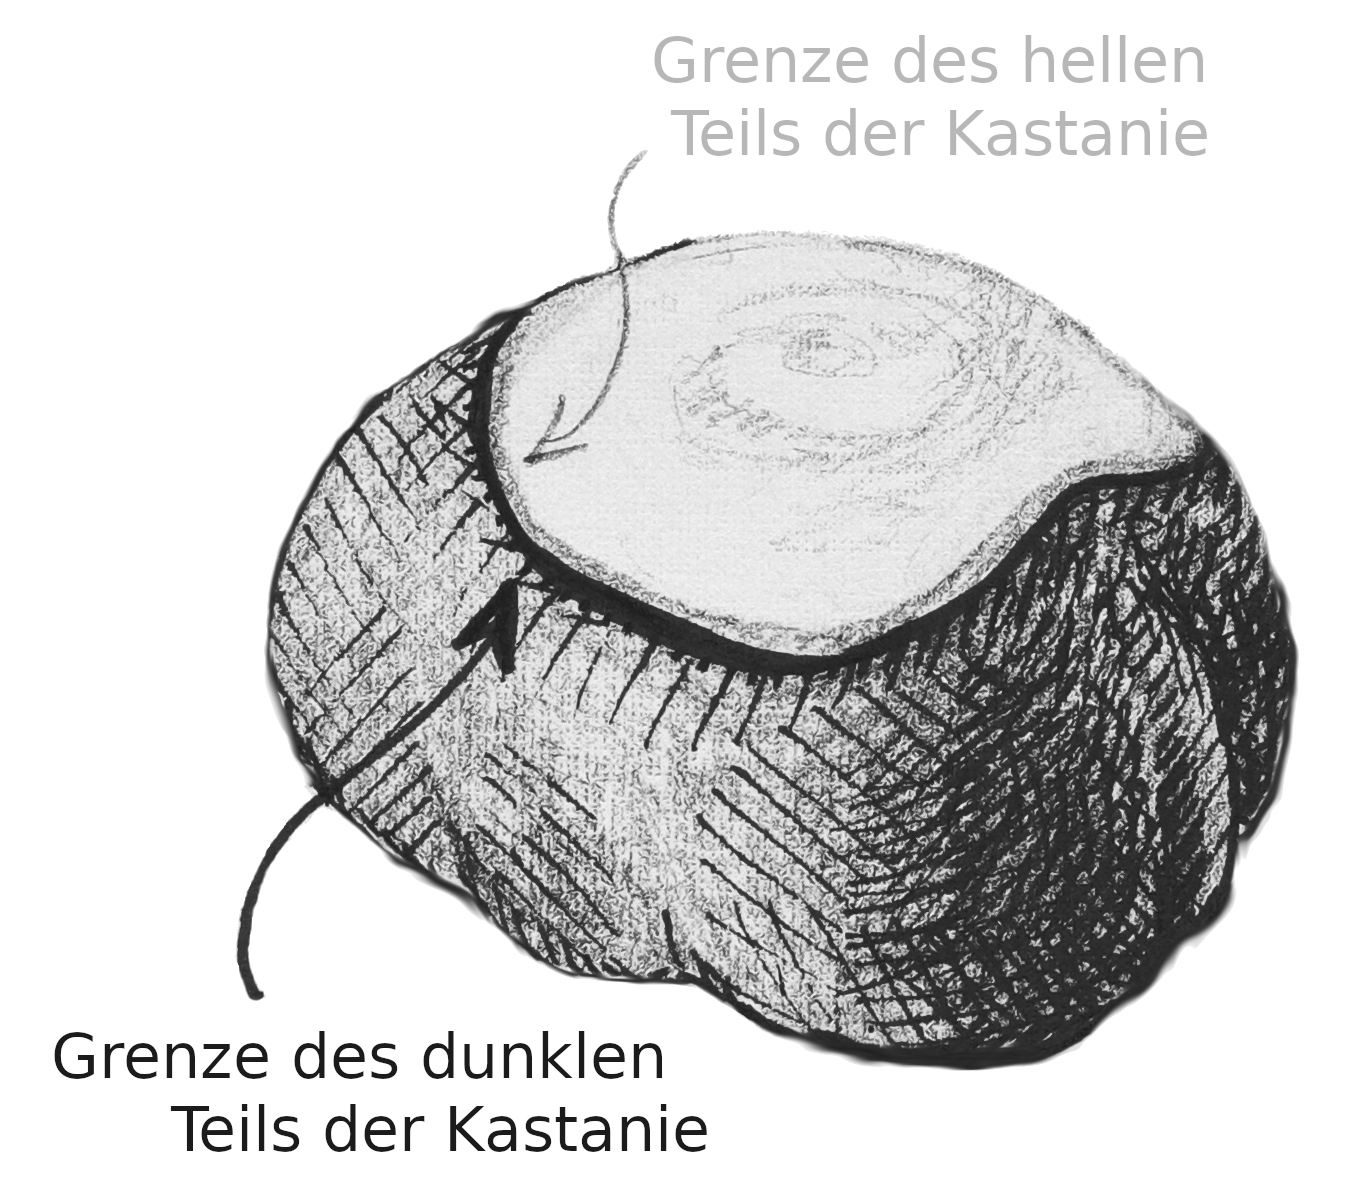
\includegraphics[height=4cm]{abb/kastanie.png}
            \caption{Jede Grenzfläche hat ihre eigenen Grenzlinien}
            \label{fig:kastanie}
        \end{figure}
        
       
 %\item \textbf{Räumlicher Teil (spatial part):}
 \paragraph{Räumlicher Teil:}
 %\paragraph{}
       Raumentitäten
       \marginpar{Räumlicher Teil}
       können Teil anderer gleichdimensionaler Raumentitäten sein.
       Sachsen ($2$-dimensional) ist beispielsweise ein Teil Deutschlands ($2$-dimensional), nicht jedoch die sächsische Grenze zwischen Sachsen und Thüringen ($1$-dimensional).
       Mit $\Gspart(x,y)$ wird ausgedrückt, dass $x$ ein räumlicher Teil von $y$ ist.
       Bei Raumregionen entspricht die $\Gspart$-Relation dem intuitiven Verständnis der Teil-von-Beziehung. 
       Der Erdkern ist beispielsweise ein Teil der Erde.
       Wenn eine niederdimensionale Raumentität $A$ eine andere begrenzt, so wird diese auch von jedem Teil von $A$ begrenzt.
       % Eine niederdimensionale Raumentität kann nur Teil einer anderen sein, wenn sie eine gleiche höherdimensionale Raumentität begrenzen.
       % Genauer gesagt: Wenn $A$ Grenze von $B$ ist und $A'$ Teil von $A$, so muss auch $A'$ Grenze von $B$ sein.
       
%\end{enumerate}


\section{Ausgewählte definierte Relationen}
In diesem Abschnitt stelle ich ausgewählte definierte Relationen der Theorie $\theoryBS$ anschaulich vor. 

    \paragraph{Räumliche Grenzen und niederdimensionale Raumentitäten:}
    %\paragraph{}
        %SB, dDE, LDE, eqdim
        Eine
        \marginpar{Räumliche Grenze,\\niederdimensional,\\gleichdimensional,\\Flächen-/Linien-/Punktregion}
        räumliche Grenze (spatial boundary) ist eine Raumentität, die eine andere begrenzt%
        \footnote{Dies ist nicht zu verwechseln mit der binären $\Gsb$-Relation, bei der $\Gsb$ auch für \glqq spatial boundary\grqq\ steht.}.
        Niederdimensionale Raumentitäten sind Raumentitäten, die keine Raumregionen sind. 
        Sie haben immer einen Teil, der eine andere Raumentität begrenzt.
        Es gibt jedoch niederdimensionale Raumentitäten, die nicht als Ganzes Grenze einer anderen sind (vgl.\ extraordinäre Raumentitäten unten).
        Raumentitäten, die einen Teil haben, der eine $n$-dimensionale Raumentität begrenzt sind $(n-1)$-dimensional ($n \in \{1,2,3\}$).
        Die $\Geqdim$-Relation besagt, dass zwei Raumentitäten die gleiche Dimension haben.
        Niederdimensionale Raumentitäten werden je nach Dimension -- in üblicher Weise -- Flächen-, Linien- oder Punktregionen genannt.
        
    \paragraph{Teile und Hyperteile:}
        %sppart, inpart, hypp, sov
        Die
        \marginpar{echter Teil,\\atomare Raumentität,\\Überlappung,\\Hyperteil,\\innerer/tangentialer Teil}
        $\Gspart$-Relation ist eine partielle Ordnung. Die zugehörige strikte partielle Ordnung (echter räumlicher Teil) wird mit $\Gsppart$ (proper spatial part) bezeichnet.
        Eine Raumentität, die keinen echten Teil besitzt, heißt atomar.
        Zwei gleichdimensionale Raumentitäten überlappen (overlap), wenn sie einen Teil besitzen, der beiden gemeinsam ist (siehe Abbildung \ref{fig:overlap}).
        Die $\Gspart$-Relation stellt eine Beziehung zwischen gleichdimensionalen Raumentitäten dar.
        Die Hyperteil-Relation hingegen drückt aus, dass eine Raumentität in einer anderem mit höherer Dimension enthalten ist.
        Je nach Dimension der niedriger-dimensionalen Raumentität spricht man von $2$-, $1$- oder $0$-dimensionalen Hyperteilen.
        Hyperteile können sowohl ganz im Inneren einer anderen Raumentität liegen als auch auf deren Rand.
        Ein innerer Teil einer Raumentität ist ein räumlicher oder ein Hyperteil, der nicht ihren Rand berührt. 
        Ansonsten spricht man von einem tangentialen Teil.
        Da Punktregionen keinen Rand haben, bestehen sie nur aus inneren Teilen.
        Innere und tangentiale Teile müssen jedoch nicht unbedingt Hyperteile sein, sondern können auch gleichdimensional und in diesem Fall räumliche Teile sein.
        Abbildung~\ref{fig:hypp} zeigt verschiedene Fälle der Hyperteil-Beziehung sowie Beispiele für innere und tangentiale Teile.
        
        %\todo[inline]{Bild hypp einscannen}
        \begin{figure}[ht]
            \centering
            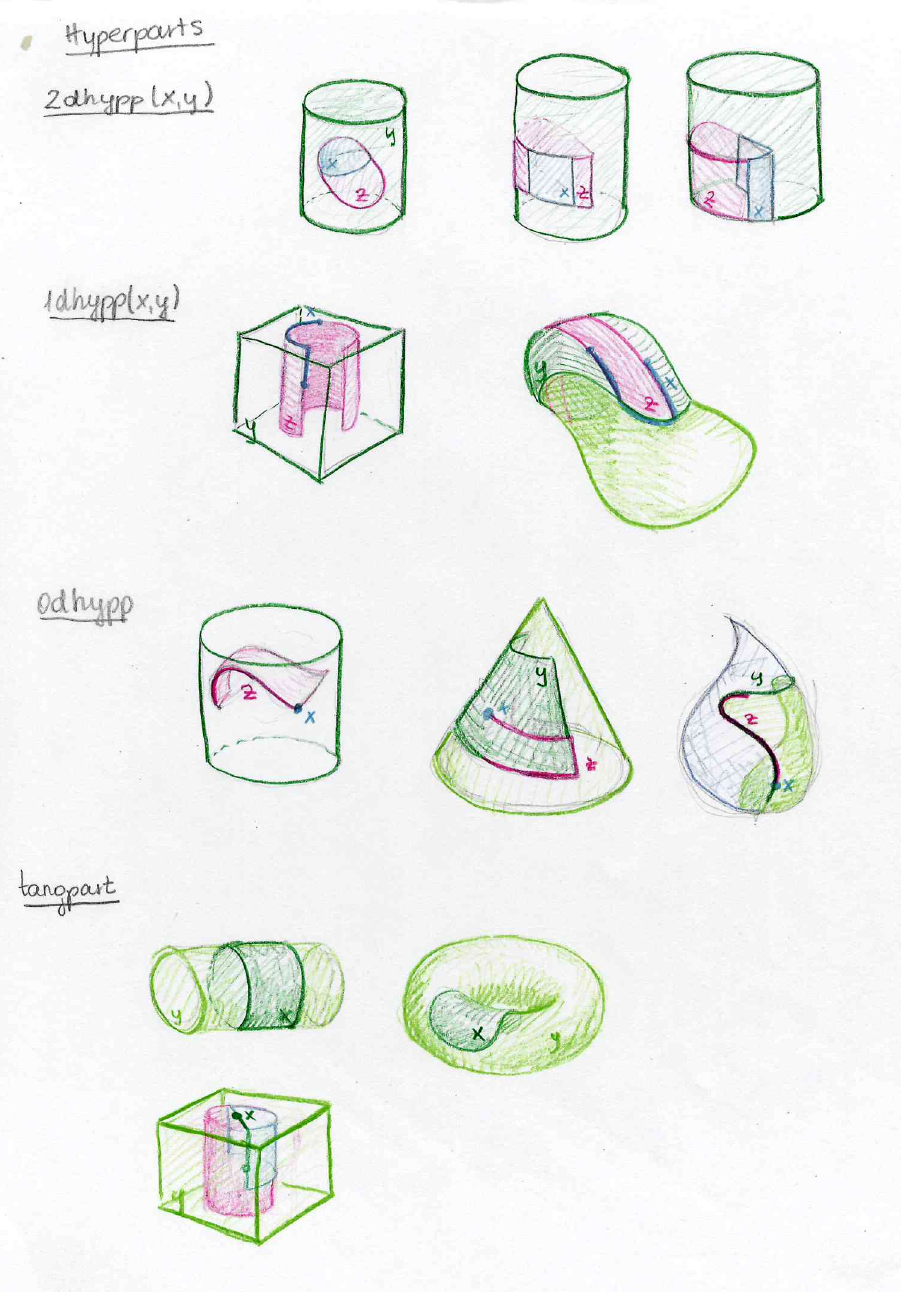
\includegraphics[width=10cm]{abb/hypp.png}
            \caption{Verschiedene Fälle von Hyperteilen}
            \label{fig:hypp}
        \end{figure}

    \paragraph{Mereologische Summe, ordinäre und extraordinäre Raumentitäten:}
        Die
        \marginpar{mereologische Summe,\\ordinär,\\extraordinär}
        mereologische Summe zweier Objekte ist eine Entität, die die gleichen Teile besitzt wie die beiden ursprünglichen.
        Beispielsweise ist die mereologische Summe von Europa und Russland die Landfläche, die Europa und Russland gemeinsam einnehmen (siehe Abbildung \ref{fig:mereologische-summe}).
        Als Spezialfall ist die mereologische Summe eines Objekts mit einem Teil von sich selbst wieder das Objekt selbst.
%         In $\BS$ können mereologische Summen nur aus Entitäten gleicher Dimension gebildet werden.
%         Wenn die beteiligten Entitäten Teile besitzen, die zwar koinzidieren, aber nicht gleich sind entstehen dabei extraordinäre Raumentitäten. 
%         Haben wir beispielsweise zwei aufeinanderliegende Würfel und betrachten die mereologische Summe ihrer Oberflächen, so koinzidert die Oberseite des unteren mit der Unterseite des oberen und es entsteht eine extraoordinäre Raumentität.
%         Zur Definition der mereologischen Summe in der Theorie $\BS$ wird die Überlappungsrelation $\Gsov(x,y)$ benutzt, die besagt, dass $x$ und $y$ einen gemeinsamen Teil haben.
%         Damit wird definiert: $\Gsum(x,y) := \fa u (\Gsov(x,u) \oder \Gsov(y,u) \leftrightarrow \Gsov(z,u))$.
        \begin{figure}[ht]
            \centering
            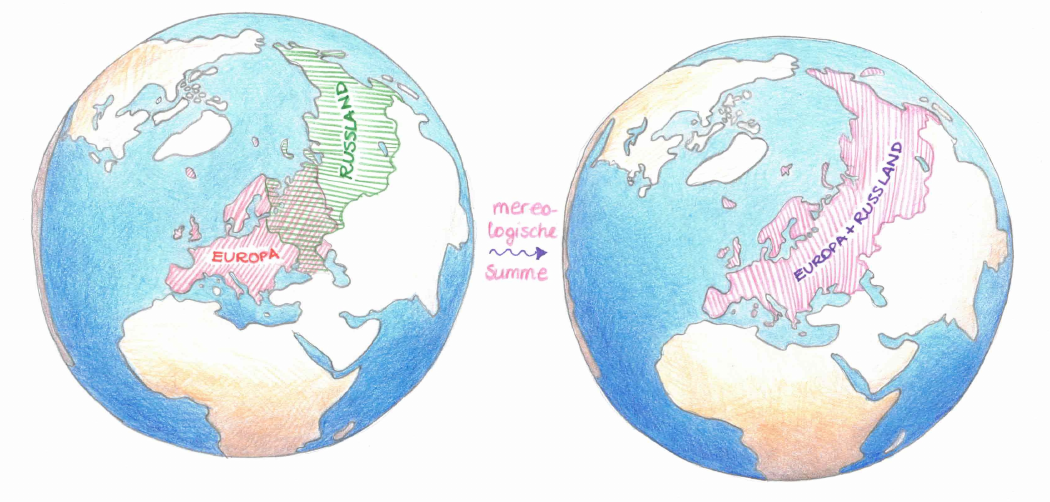
\includegraphics[width=\textwidth]{abb/mereologische-summe.png}
            \caption{Mereologischen Summe von Flächenregionen}
            \label{fig:mereologische-summe}
        \end{figure}
        %
		Raumregionen und räumliche Grenzen sind ordinäre Raumentitäten.
		Die Theorie fordert die uneingeschränkte Existenz der mereologischen Summe gleichdimensionaler Entitäten. Dadurch können extraordinäre Raumentitäten entstehen. Das sind Raumentitäten, die Teile haben, die koinzidieren, aber nicht überlappen.
		Nehmen wir die Oberflächen zweier übereinanderliegenden Würfel. 
		Die obere Fläche des unteren Würfels koinzidiert mit der unteren Fläche des oberen Würfels. Die beiden Flächen haben jedoch keine Teile gemeinsam, da die erste von unten, die zweite von oben erzeugt wird. 
		Mit anderen Worten: Sie überlappen nicht. Damit ist ihre mereologische Summe eine extraordinäre Raumentität.
		Ein ähnliches Beispiel ist in Abbildung \ref{fig:extraordinaer} dargestellt.
		%
		%\todo[inline]{Bild extraordinaer einscannen}
        \begin{figure}[ht]
            \centering
            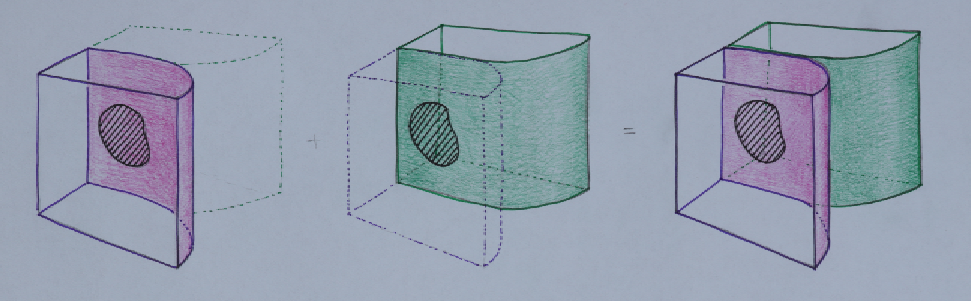
\includegraphics[width=\textwidth]{abb/extraordinaer.png}
            \caption[Eine extraordinäre Raumentität als Summe zweier ordinärer Flächenregionen]{Eine extraordinäre Raumentität als Summe zweier ordinärer Flächenregionen.\\
            Die schraffierten Teile koinzidieren, überlappen jedoch nicht.}
            \label{fig:extraordinaer}
        \end{figure}
        %
		Diese Konstruktion mag auf den erste Blick künstlich erscheinen, es lassen sich jedoch auch im Alltag Beispiele finden, die belegen, dass es sinnvoll ist, von der Existenz extraordinärer Raumentitäten auszugehen. 
		Man nehme beispielsweise ein Buch. 
		Zugeklappt erscheint es bei erster Betrachtung als Quader. 
		Wichtiger ist jedoch, was auf den Seiten steht, d.\,h.\ nicht der Quader und eigentlich auch nicht die Buchseiten, sondern die Oberfläche der Buchseiten sind das Interessante an diesem Objekt. 
		Diese Oberflächen koinzidieren für je zwei gegenüberliegende Seiten.
		Selbstverständlich macht es keinen Sinn, diese koinzidierenden Flächen zu identifizieren, da sie verschiedene Informationen enthalten. 
		Die Oberfläche eines Buches als mereologische Summe der Oberfläche seiner Seiten besitzt also jede Menge koinzidierender nichtgleicher Teile und ist somit eine extraordinäre Raumentität.
        %
		Da Raumregionen nicht koinzidieren können, sind sie immer ordinär.

    \paragraph{Zusammenhang:}
        Zusammenhängende
        \marginpar{($d$-dimensional) zusammenhängend} 
        Raumentitäten sind Raumentitäten, in denen -- anschaulich gesprochen -- je zwei Punkte (als Hyperteile) durch einen \glqq Weg\grqq\ in ihrem Inneren verbunden werden können.
        Je nach Art der \glqq schwächsten\grqq\ Verbindungsstelle unterscheiden wir $2$-, $1$- und $0$-dimensional zusammenhängende Raumentitäten (siehe Abbildung \ref{fig:zusammenhang}).
        Genauer gesagt: Eine Raumentität ist $d$-dimensional zusammenhängend, wenn jeder Schnitt, der sie in zwei Teile zerlegt, mindestens Dimension $d$ hat.%
        \footnote{
            Dieser Zusammenhangsbegriff ist nicht zu verwechseln mit dem topologischen Begriff des $d$-Zusammenhangs, der auf Homotopieklassen beruht.
        }
        Jede $d$-dimensional zusammenhängende Raumentität ist also auch ($d$-1)-dimensional zusammenhängend.
        Man beachte, dass Raumregionen auch dann $d$-dimensional zusammenhängend sein können, wenn sie lokal Stellen mit schwächerem Zusammenhang haben. Dieses Konzept wird im Anhang \ref{sec:lok-zusammenhang} als Nebenresultat formalisiert. Siehe hierzu auch das Beispiel für eine $1$-dimensional zusammenhängende Flächenregion in Abbildung \ref{fig:zusammenhang}.

        \begin{figure}[ht]
            \centering
            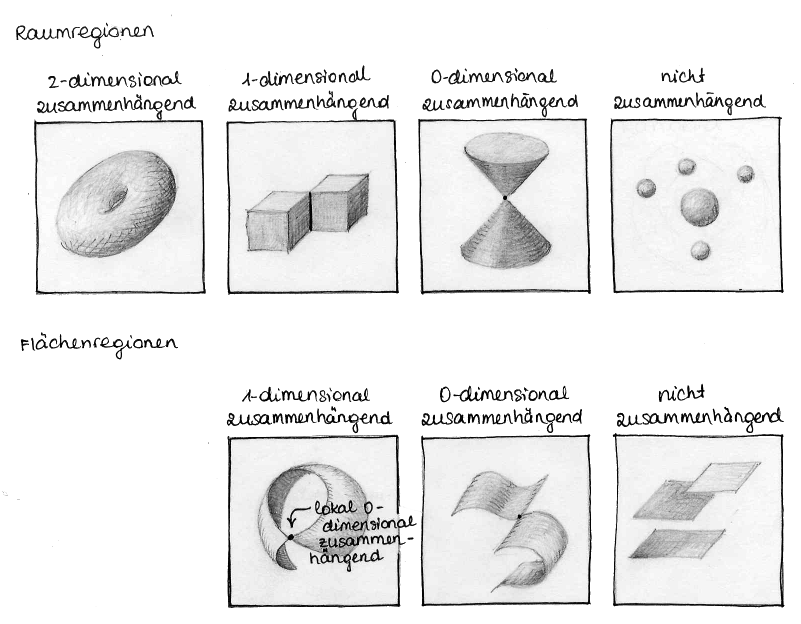
\includegraphics[width=\textwidth]{abb/zusammenhang_2.png}
            \caption{Verschieden zusammenhängende Raumentitäten}
            \label{fig:zusammenhang}
        \end{figure}
    
    \paragraph{Topoide, Flächen, Linien und Punkte:}
        Eine
        \marginpar{Topoid,\\Fläche,\\Linie,\\Punkt}
        $2$-dimensional zusammenhängende Raumregion heißt Topoid (topoid).
        Eine $1$-di\-men\-sional zusammenhängende ordinäre Flächenregion heißt Fläche (surface).
        Eine zusammenhängende ordinäre Linienregion heißt Linie (line).
        Eine atomare %\footnote{Eine Entität ist atomar, wenn sie keine echten Teile besitzt (d.h., wenn sie nur sich selbst als Teil besitzt).} 
        Punktregion heißt Punkt (point).
        Topoide, Flächen, Linien und Punkte sind die Raumentitäten, die unserer Intuition am nächsten kommen.
        Sie sind ordinär
        %\footnote{Man beachte, dass Raumregionen und atomare Raumentitäten immer ordinär sind.}
        und global gesehen maximal-dimensional zusammenhängend.
        Man beachte jedoch, dass sie lokal möglicherweise schwächer zusammenhängend sein können, wie in Abbildung \ref{fig:zusammenhang} das Beispiel für eine $1$-dimensional zusammenhängende Flächenregion.


\section{Axiome}\label{ssec:axiome}
$\theoryBS$ liegt als Axiomatisierung in 33 Axiomen vor, die auf den Übersichtsblättern (Übersicht 1) aufgelistet sind.
In diesem Abschnitt fasse ich ihre wichtigsten Aussagen zusammen.

Die
%\marginpar{Grundlegende Taxonomie und Existenz,\\$\Gspart$}
\marginpar{A1--A3}
ersten Axiome (A1--A3) stellen sicher, dass es Raumentitäten gibt und dass diese je nach Dimension in vier paarweise disjunkte Klassen zerfallen.
A4--A7
%\marginpar{Mereologische Überlegungen}
\marginpar{A4--A7}
garantieren, dass die $\Gspart$-Relation eine Äquivalenzrelation für gleichdimensionale Raumentitäten ist.


Wenn
%\marginpar{Starkes Ergänzungsprinzip}
\marginpar{A8}
eine Raumentität $A$ eine andere ($B$) nicht komplett einschließt%
\footnote{im Sinne der $\Gspart$-Relation},
so gibt es einen Rest -- also eine Raumentität, die Teil von $A$ ist und nicht mit $B$ überlappt (siehe Abbildung \ref{fig:supplementation}).
Diese Eigenschaft heißt starkes Ergänzungsprinzip (strong supplementation principle) und wird in A8 formalisiert.

\begin{figure}[ht]
    \centering
    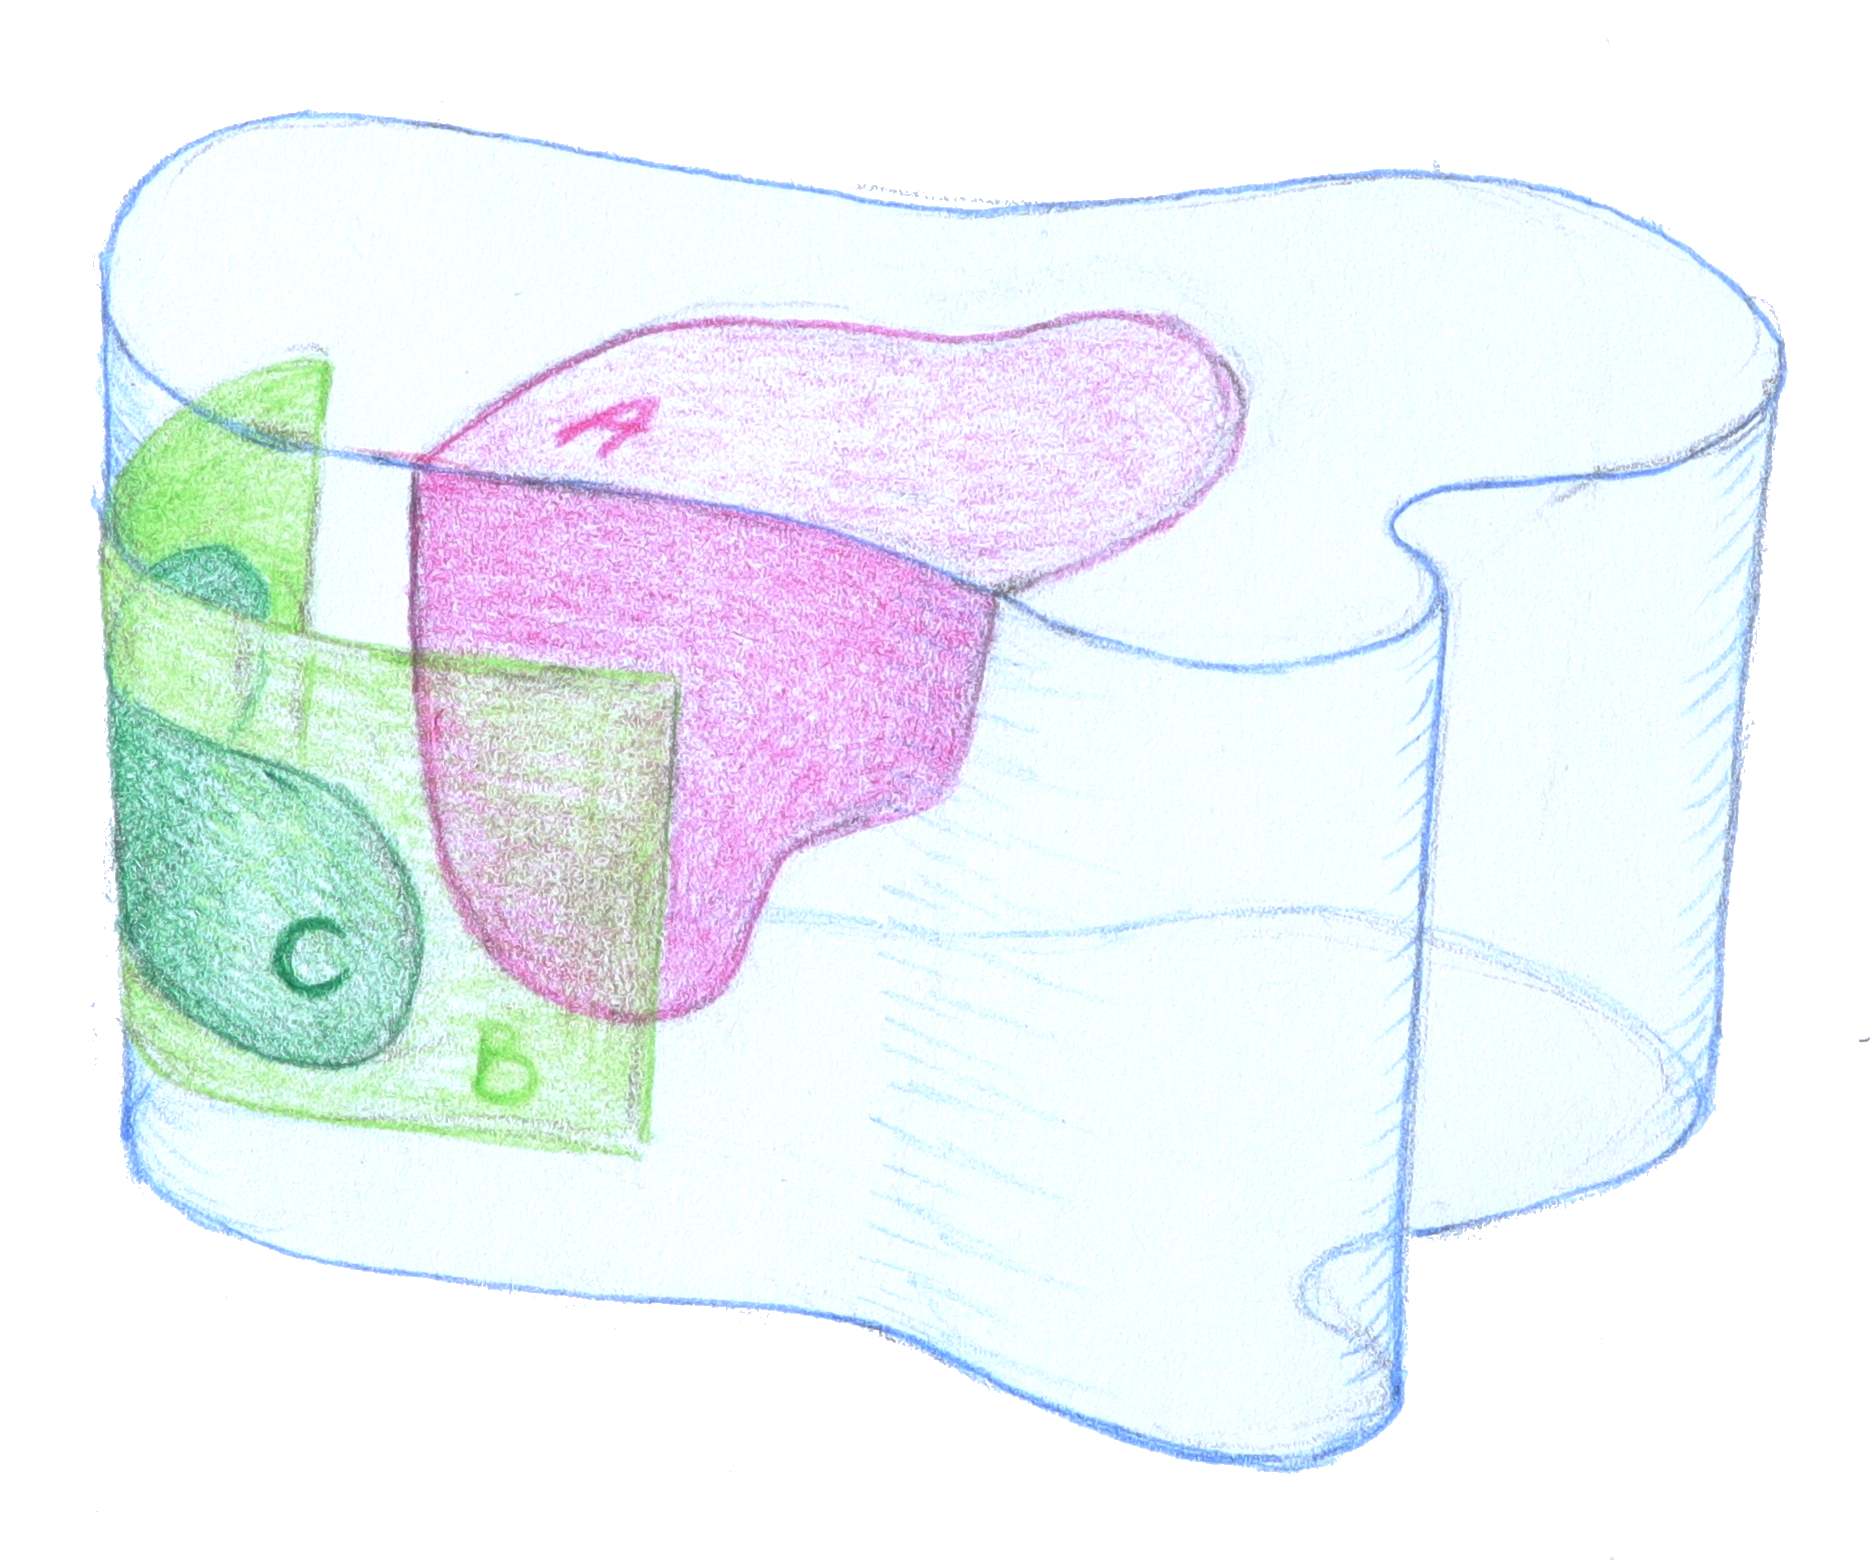
\includegraphics[height=5cm]{abb/supplementation.png}
    \caption[Zum starken Ergänzungsprinzip]{Zum starken Ergänzungsprinzip: $A$ ist nicht Teil von $B$, deshalb gibt es einen Teil $C$ von $B$, der nicht mit $A$ überlappt.}
    \label{fig:supplementation}
\end{figure}

% Intuitively, this says that if an object fails to include another among its parts, then there must be a remainder, something that makes up for the difference. 

A9--A10
%\marginpar{Einschränkung und Erweiterung von Raumentitäten}
\marginpar{A9--A10}
sorgen dafür, dass jede Raumentität -- mit Ausnahme von Punktregionen -- einschränkbar und erweiterbar ist. D.\,h., sie besitzt einen echten inneren Teil und ist in eine echt größere einbettbar. Letzteres gilt auch für Punktregionen.
Zusammen mit A1 ergibt sich daraus insbesondere, dass jedes $\theoryBS$-Modell unendlich ist.

A11--A18
%\marginpar{Existenz von Raumentitäten} 
\marginpar{A11--A18}
sind Existenzaxiome. 
Sie garantieren, dass jede Raumregion in ein Topoid einbettbar ist und geben Bedingungen für die Existenz (größter) räumlicher Grenzen, der mereologischen Summe, des Schnitts und des relativen Komplements zweier Raumentitäten an.
Hervorzuheben ist hierbei Axiom A16, das die uneingeschränkte Existenz mereologischer Summen für gleichdimensionale Raumentitäten fordert.

Dass
%\marginpar{$\Gscoinc$}
\marginpar{A19--A22}
die $\Gscoinc$-Relation auf gleichdimensionalen räumlichen Grenzen eine Äquivalenzrelation ist, wird durch die Axiome A19--A22 ausgedrückt.

A23
%\marginpar{$\Gsb$}
\marginpar{A23--A30}
besagt, dass ordinäre Raumentitäten ordinäre Grenzen haben.
A24 garantiert, dass Teile von Grenzen wieder Grenzen der selben Raumentitäten sind.
A25 und A26 enthalten weitere Aussagen über die $\Gsb$-Relation.
A25 hat einen wichtigen Einfluss auf die Definition der Objektäquivalenz in Kapitel~\ref{chap:bso-struktur}, die die Grundlage des vorgestellten Interpretationsansatzes bildet.
Es hat zur Folge, dass eine Raumentität $A$, die eine zweite ($B$) begrenzt, auch jede andere Raumentität begrenzt, die \glqq aus dem Inneren von $B$ auf $A$ zukommt\grqq .
Siehe hierzu Abbildung \ref{fig:A25}.
A27--A30
%\marginpar{Koinzidenz und unterscheidbare Hyperteile}
geben Eigenschaften der $\Gspart$- und $\Ghypp$-Relation an.


    \begin{figure}[ht]
        \centering
        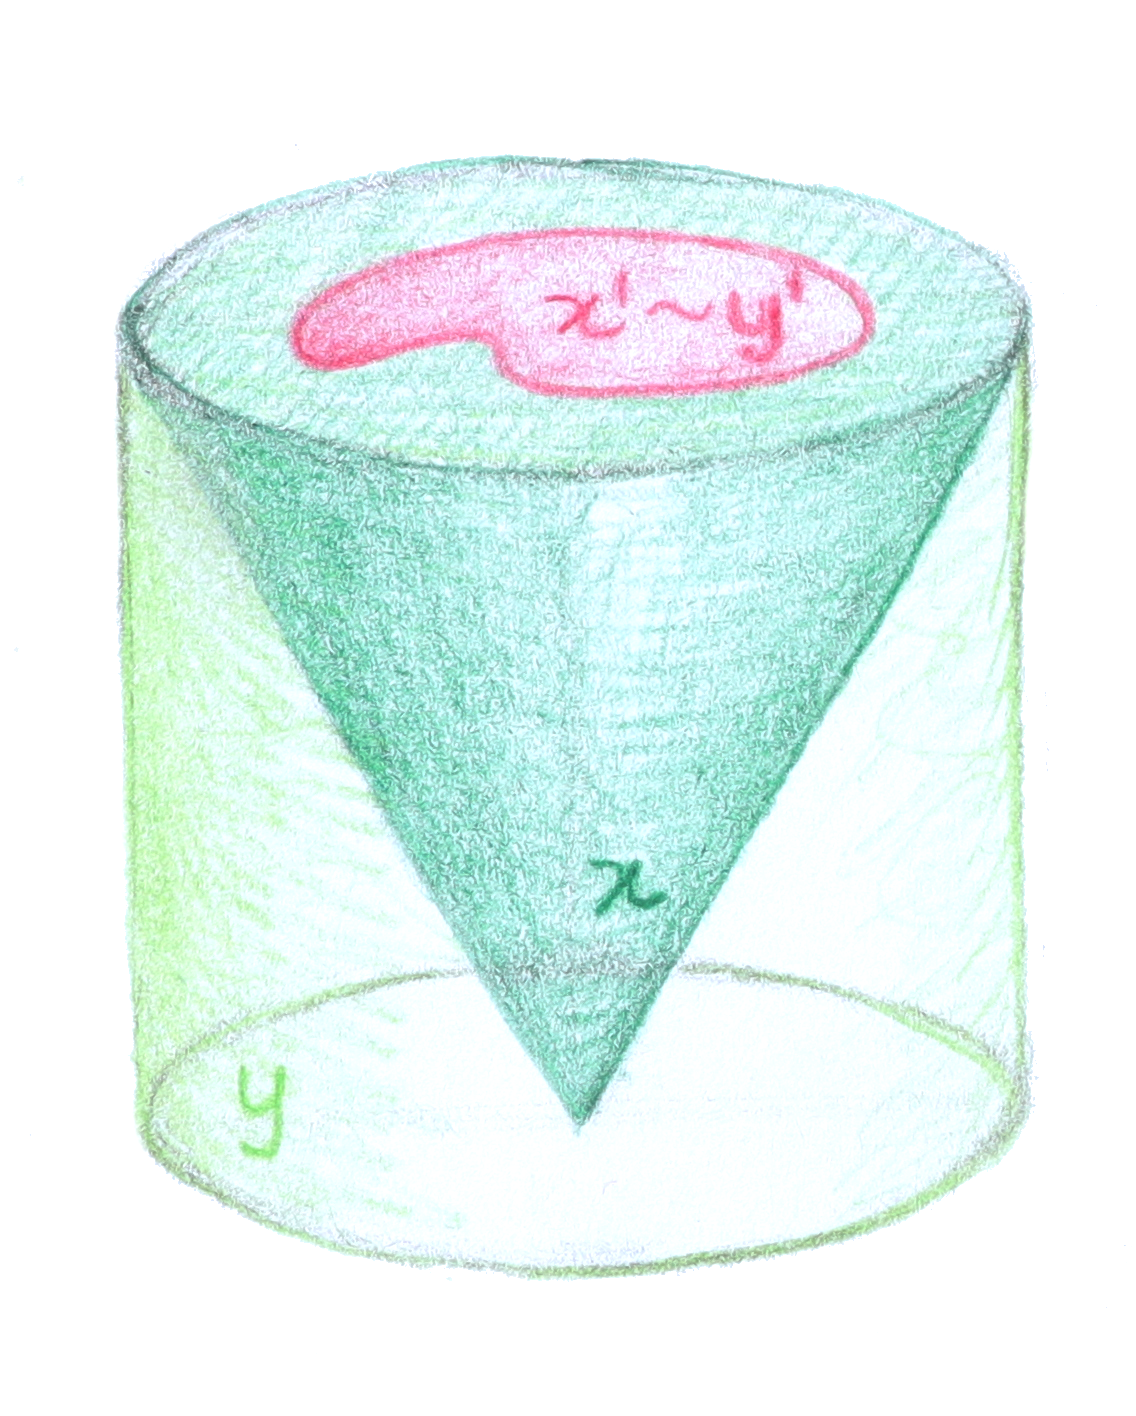
\includegraphics[height=5cm]{abb/a25.png}
        \caption[Zu Axiom 25]{Zu Axiom A25: Wenn $x$ in $y$ liegt und $x'$ (Grenze von $x$) und $y'$ (Grenze von y) koinzidieren, so begrenzt $x'$ auch $y$.}
        \label{fig:A25}
    \end{figure}
    
    In
    %\marginpar{(Un)Gleichheit von räumlichen Grenzen}
    %\marginpar{A31--A33}
    einem 2019 von denselben Autoren veröffentlichten Konferenzpapier [\cite{baumann-r-2019--a}] werden drei weitere Axiome eingeführt, die wichtige Vorstellungen widerspiegeln, die dem hier vorgestellten Interpretationsansatz zugrunde liegen.
    
    Nach
    \marginpar{A31}
    Axiom A31 besitzen Raumentitäten, die eine gemeinsame Grenze haben, einen gemeinsamen echten Teil an dieser Grenze.
    
    Der
    \marginpar{Korrekturen zu A32}
    Erläuterung zu A32 in [\cite{baumann-r-2019--a}] entsprechend zielt Axiom A32
		analog auf eine Art Umkehrung von A31 ab,
		indem an unterschiedlichen Grenzen die begrenzten Entitäten disjunkte Teile 
		mit diesen Grenzen aufweisen sollen.
    %\marginpar{Diskussion zu Axiom A32}
    A32 muss jedoch formal modifiziert werden, da es in der gegebenen Form nicht der intendierten Aussage entspricht. Ein problematischer Fall ist in Abbildung \ref{fig:a32} dargestellt.
    
    \begin{figure}[ht]
        \centering
        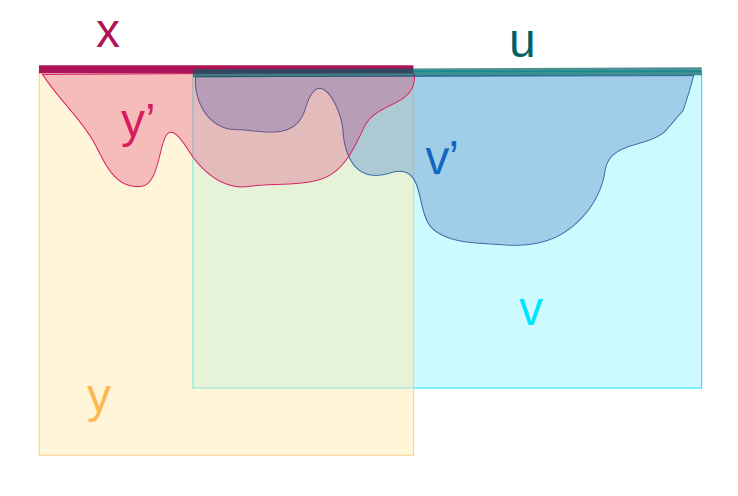
\includegraphics[height=3.5cm]{abb/a32.png}
        \caption[Zu Axiom 32]{Zu Axiom A32: Zwei Grenzen, für die je zwei Raumentitäten, die von ihnen begrenzt werden, überlappen}
        \label{fig:a32}
    \end{figure}
    
    In der ursprünglichen Version lautet das Axiom:
%     \begin{align*}
%         &\Gsb(x,y) \land \Gsb(u,v) \land x\neq u \to\\ 
%         &\exists y'v'\:(\: \Gspart(y',y) \land \Gsb(x,y') \land \Gspart(v',v) \land \Gsb(u,v') \land \neg \Gsov(y',v'))
%     \end{align*}
    \begin{align*}
        \Gsb(x,y) \land \Gsb(u,v) \land x\neq u &\to\: 
        \exists y'v'\:(\: \Gspart(y',y) \land \Gsb(x,y') 
        \land \mbox{} \\
        &\Gspart(v',v) 
        \land \Gsb(u,v') \land \neg \Gsov(y',v'))
    \end{align*}

    
    Angenommen, es gibt Raumentitäten $x$, $y$, $u$ und $v$ mit $\Gsb(x,y)$, $\Gsb(u,v)$, $x \neq u$ und $\Gsov(x,u)$ und A32 gilt.
    Seien $y'$ und $v'$ Raumentitäten mit $\Gspart(y',y)$, $\Gsb(x,y')$, $\Gspart(v',v)$, $\Gsb(u,v')$ und $\neg \Gsov(y',v')$.
    Nach der Definition von $\Gsov$ gibt es eine Raumentität $z$ mit $\Gspart(z,x)$ und $\Gspart(z,u)$.
    Damit gelten nach Axiom A24
    %\marginpar{FL, 22.04.: TODO\\neu A24 war A23 - bitte nochmal checken} 
    $\Gsb(z,y')$ und $\Gsb(z,v')$ und somit existiert nach Axiom A31 eine Raumentität $w$ mit $\Gsppart(w,y')$ und $\Gsppart(w,v')$.
    Also überlappen $y'$ und $v'$. $\lightning$
    
    Deshalb schlage ich vor, $x \neq u$ zu $\neg \Gsov(x,u)$ zu verschärfen.
% 
% $$\Gsb(x,y) \wedge \Gsb(x,z) \to
%              \exists u (\Gsb(x,u) \land \Gsppart(u,y) \land \Gsppart(u,z))$$
% % 				 \label{ax:cbspp}}
% %        {entities with a common boundary share a proper part at that boundary}	
% % 						
% % 						
% % \itemTP{ \mbox{}$\\
% % \hspace*{1em}
% %
% $$\Gsb(x,y) \land \Gsb(u,v) \land x\neq u \to \exists y'v'\:(\: \Gspart(y',y) \land \Gsb(x,y') \land \Gspart(v',v) \land \Gsb(u,v') \land \neg \Gsov(y',v')) $$
% 			  \label{ax:dbipno}}
%        {entities with distinct boundaries have parts at those boundaries
% 			  that do not overlap}
% 				
% \itemTP{$\GLDE(x) \Land \GOrd(x) \Limp \GSB(x)$\\ \mbox{}

    A33
    %\marginpar{Ordinäre Raumentitäten und Grenzen}
    \marginpar{A33}
    schließlich besagt, dass alle ordinären niederdimensionalen Raumentitäten räumliche Grenzen sind.
    Damit sind die Forderungen
    \begin{enumerate}
     \item \glqq Alle Raumentitäten sind ordinär.\grqq\ und
     \item \glqq Alle niederdimensionalen Raumentitäten sind räumliche Grenzen.\grqq
    \end{enumerate}
    äquivalent.


    
\section{Die Theorie der ordinären Raumentitäten}\label{sec:bso}
Um die Konstruktion eines Modells zu erleichtern, führe ich in dieser Arbeit die vereinfachte Raumtheorie $\theoryBSO$ ein, die nur räumliche Grenzen als niederdimensionale Raumentitäten zulässt.
% \cFLs Die Ontologie $\BS^O$ ist eine Vereinfachung von $\BS$, die nur räumliche Grenzen als niederdimensionale Raumentitäten zulässt.\cFLimp{Einstieg anpassen: Ab hier neue Definition von $\BS^O$ und weswegen, dann die eigentliche Darstellung/Einführung von $\BS^O$}
Unter dieser Voraussetzung besteht das Diskursuniversum nur aus Raumregionen und räumlichen Grenzen.
Aus Axiom A23, das besagt, dass räumliche Grenzen von ordinären Raumentitäten wieder ordinär sind, folgt damit, dass alle Raumentitäten ordinär sind.
% Wenn alle niederdimensionalen Raumentitäten räumliche Grenzen sind,
% das Diskursuniversum also nur aus Raumregionen und räumlichen Grenzen besteht,
% dann sind alle Raumentitäten ordinär.
% Dies ist im Wesentlichen eine Folgerung aus Axiom A23, das besagt, dass räumliche Grenzen von ordinären Raumentitäten wieder ordinär sind.
Deshalb ist $\theoryBSO$ die Theorie der ordinären Raumentitäten.

Da durch mereologische Summenbildung extraordinäre Raumentitäten entstehen können, muss die Gültigkeit von Axiom A16 eingeschränkt werden, das die Existenz der mereologischen Summe für gleichdimensionale Raumentitäten fordert.

%\paragraph{Axiomatisierung}\ \\
\subsection{Axiomatisierung}
$\theoryBSO$ entsteht aus $\theoryBS$ durch die Hinzunahme eines weiteren Axioms
$$\text{A0.} \quad \GLDE(x) \to \GSB(x)$$
und Modifikation von A16 zu
\begin{align*}
 \text{A16'.} \quad \Geqdim(x,y) \wedge \mbox{} &\neg \exists x'y'\ (\Gspart(x',x) \wedge \Gspart(y',y) \wedge \mbox{} \\
 &\Gscoinc(x',y') \wedge \neg \Gsov(x',y')) \to \exists z\ \Gsum(x,y,z)
\end{align*}

%\todo[inline]{\small FL n03.05. mini\\
%$\neg sov(x,y)$ in A16' könnte vor die mit $\neg \exists x' y'$ beginnende Teilformel gezogen werden, da dieses Literal nur $x$ und $y$ betrifft.
%Fiel mir nur neu auf; bei Änderung erneute Angabe am Ende von 2.4 beachten.\\
%-> BH: Ich denke, du hast da eher einen Fehler entdeckt und es müsste $\neg sov(x',y')$ heißen}
A16' besagt, dass die Existenz der mereologischen Summe zweier gleichdimensionaler Raumentitäten dann garantiert ist, wenn diese keine koinzidierenden, nichtüberlappenden Teile besitzen -- wenn also durch die Summenbildung keine extraordinäre Raumentität entsteht.
Ob diese Einschränkung ausreicht und ob gegebenenfalls noch weitere Axiome eingeschränkt werden müssen, ist noch zu untersuchen (vgl.\ dazu die Diskussion in Abschnitt \ref{sec:offene-fragen}).

Abbildung \ref{fig:summe-linien} zeigt ein Beispiel für die mereologische Summe zweier Linienregionen, die nicht extraordinär ist und somit auch nach Axiom A16' existiert.
Dargestellt sind zwei Linienregionen $x$ und $y$, die die Flächenregionen $x'$ und $y'$ begrenzen.
Ihre mereologische Summe ist wiederum Grenze einer Raumentität $z'$, die sich jedoch nicht durch einfache Mengenoperatoren aus $x'$ und $y'$ konstruieren lässt.
Allerdings gilt, dass $x$ und $y$ auch $z'$ begrenzen.

\begin{figure}[ht]
    \centering
    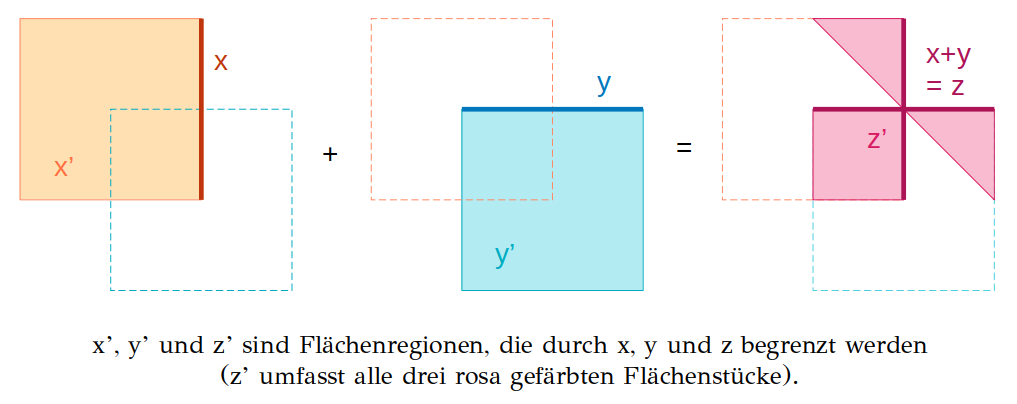
\includegraphics[width=0.9\textwidth]{abb/summe-linien.png}
    \caption{Beispiel für die mereologische Summe zweier Linienregionen, die \textit{nicht} extraordinär ist}
    \label{fig:summe-linien}
\end{figure}

%\todo[inline]{\small FL n03.05. mini\\
%Im Text in Abb.\ \ref{fig:summe-linien} ``rosa gefärbte'' $\to$ ``rosa gefärbten''\\
%-> BH: done}
Als Folgerung aus dem neuen Axiom A0 und den alten Axiomen A2, A3 und A23 sowie den Definitionen D22 und D23 ergibt sich, dass in $\theoryBSO$ alle Raumentitäten ordinär sind. $\theoryBSO$ enthält also als zusätzliches Theorem
$$ \GOrd(x). $$
Dadurch ist das Konzept ordinärer Raumentitäten in der Theorie $\theoryBSO$ trivialisiert. Insgesamt bietet sich aus derartigen Gründen eine Modifikation der Theorie an.

%\paragraph{Modifizierte Formalisierung}\ \\
\subsection{Modifizierte Formalisierung}
Durch die Einschränkung von $\theoryBS$ auf $\theoryBSO$ werden einige Definitionen vereinfacht bzw. überflüssig, da sie triviale Konzepte definieren oder da definierte Konzepte zusammenfallen.
Dies führt auch dazu, dass Axiome umgeschrieben werden müssen, die besagte Konzepte enthalten. 
Andere werden tautologisch und können deshalb entfallen.
Eine vollständige Liste aller Symbole und Axiome findet sich auf den beiliegenden Übersichtsblättern (Übersicht 2).

%\paragraph{Definitionen}\ \\
D7 und D8 sind redundant, weil $\GLDE$ mit $\GSB$ und $\GdDE$ mit $\GdDB$ zusammenfallen.\\
Durch Ersetzung von $\GdDE$ durch $\GdDB$ wird aus D9
\begin{align*}
 \text{D9'.} \quad \Geqdim(x) := 
      &(\GSReg(x) \wedge \GSReg(y)) \vee (\GtwoDB(x) \wedge \GtwoDB(y)) \vee \mbox{} \\ 
			&(\GoneDB(x) \wedge \GoneDB(y)) \vee (\GzeroDB(x) \wedge \GzeroDB(y))
\end{align*}
%
D22 und D23 können gestrichen werden, da $\GExOrd$ und $\GOrd$  in $\theoryBSO$ triviale Konzepte sind.\\
%
Die Definitionen für Topoid, Fläche, Linie und Punkt vereinfachen sich zu  
%
\begin{align*}
 &\text{D30'.} \quad \GTop(x) := \GSReg(x) \wedge \GtwoDC(x)\\
 &\text{D31'.} \quad \GtwoD(x) := \GtwoDB(x) \wedge \GoneDC(x)\\
 &\text{D32'.} \quad \GoneD(x) := \GoneDB(x) \wedge \GzeroDC(x) \\
 &\text{D33'.} \quad \GzeroD(x) := \GzeroDB(x) \wedge \neg \exists y\ \Gsppart(y,x)
\end{align*}
%
%\paragraph{Axiome}\ \\
%Durch die Ersetzung von $\GLDE$ durch $\GSB$, $\GExOrd$ durch $\bot$ und $\GOrd$ durch $\top$ verändern sich einige Axiome bzw. sie werden überflüssig.
%
Das in diesem Abschnitt eben erst eingeführte zusätzliche Axiom A0 kann wegfallen, wenn $\GLDE$ durch $\GSB$ ersetzt wird.\\
%
A2 und A3 werden zu
\begin{align*}
 &\text{A2'.} \quad \GSB(x) \leftrightarrow \neg \GSReg(x)\\
 &\text{A3'.} \quad \neg \exists x\ ((\GtwoDB(x) \wedge \GoneDB(x)) \vee (\GtwoDB(x) \wedge \GzeroDB(x))\\
 &\phantom{\text{A3'.} \quad \neg \exists x\ ((} \vee (\GoneDB(x) \wedge \GzeroDB(x)))
\end{align*}
%
A13 und A14 müssen modifiziert werden und A15 vereinfacht sich zu
\begin{align*}
 &\text{A13'.} \quad \GtwoDB(x) \to \exists yz\ (\Gsppart(y,x) \wedge \Gsb(y,z))\\
 &\text{A14'.} \quad \GoneDB(x) \to \exists yz\ (\Gsppart(y,x) \wedge \Gsb(y,z))\\
 &\text{A15'.} \quad \exists y\ \Gsb(y,x) \to \exists z\ \Ggrsb(z,x)
\end{align*}
%
A16 wird nicht vereinfacht, sondern die Bedingung für die Existenz der mereologischen Summe wird verschärft zu dem schon erwähnten Axiom
\begin{align*}
 \text{A16'.} \quad \Geqdim(x,y) \wedge &\neg \exists x'y'\ (\Gspart(x',x) \wedge \Gspart(y',y) \wedge \\
 &\Gscoinc(x',y') \wedge \neg \Gsov(x',y')) \to \exists z\ \Gsum(x,y,z)
\end{align*}
%
A23 ($\Gsb(x,y) \wedge \GOrd(x) \to \GOrd(y)$) schließlich lässt sich ersatzlos streichen.

% 
% % \chapter{Von der Theorie $\theoryBSO$ zu einem Interpretationsansatz}
%\chapter{Grundideen des Interpretationsansatzes}\label{chap:bso-grundideen}
\chapter{Grundlagen der \strukt}\label{chap:bso-grundideen}

    In diesem Kapitel wird dargestellt, wie ich von der in Kapitel~\ref{chap:bs} eingeführten Theorie der ordinären Entitäten des Brentanoraumes zur \strukt, einer Interpretation für $\theoryBSO$, komme.

    In den Abschnitten \ref{sec:raumreg} bis \ref{sec:zusammenfassung} greife ich die dort eingeführten Ideen auf. In diesem Kapitel stehen jedoch die Vorstellungen, die meinen Interpretationsansätzen zugrunde liegen, im Mittelpunkt. Redundanzen lassen sich hierbei nicht vermeiden und werden der Abgeschlossenheit der Darstellung zuliebe in Kauf genommen.

    In den Abschnitten \ref{sec:universum} und \ref{sec:prim-rel-1} wird die \strukt eingeführt.
    Für eine exakte Ausformulierung der darin verwendeten Begriffe werden etablierte Werkzeuge aus der Topologie und weitere topologische Definitionen benötigt, die in den folgenden Kapiteln bereitgestellt werden.
    Deshalb beschränke ich mich erst einmal auf die Darstellung der grundlegenden Ideen.
    Auch für eigentlich mathematische Begriffe wie \glqq Dimension\grqq\ verlasse ich mich hier auf das intuitive Verständnis des Lesers.

    Die Lücken des vorgestellten Ansatzes werden in Abschnitt \ref{sec:ausblick} zusammengefasst und deren Lösungen in Ausblick gestellt.

    \section{Raumregionen}\label{sec:raumreg}
        Ich betrachte den Raum --~hier auch als einbettender Raum bezeichnet~-- als homogenen, unendlich ausgedehnten unveränderlichen Rahmen, in dem sich physikalische Prozesse abspielen.
        Dies steht im Widerspruch zu der in [\cite{baumann-r-2016-53-a}] vertretenen Vorstellung, dass der Raum von materiellen Objekten, die ihn einnehmen, generiert wird.
%         Dies steht möglicherweise im Widerspruch zu den Weltbild der Autoren der $\theoryBS$-Theorie,
%         die davon ausgehen, dass der Raum von materiellen Objekten, die ihn einnehmen, generiert wird.
        Für das Ziel der Arbeit, einen Ansatz für einen konstruktiven Konsistenzbeweis für $\theoryBS$ vorzustellen, sind diese Unterschiede, soweit ich es absehen kann, jedoch nicht relevant.

        Teilmengen des einbettenden Raumes, die von materiellen Körpern eingenommen werden können, heißen Raumregionen.
        \marginpar{Raumregionen und Topoide}
        Da materielle Körper endlich sind, müssen sie beschränkt sein, nicht jedoch notwendigerweise zusammenhängend, wie im vorherigen Kapitel ausgeführt wurde. 
        Zusammenhängende Raumregionen%
        \footnote{
            genauer gesagt $2$-dimensional zusammenhängende
        }
        heißen Topoide.
	
        Im Gegensatz zu materiellen Körpern können sich Raumregionen gegenseitig durchdringen,
        da jede \textit{mögliche} Teilmenge des einbettenden Raumes, die von materiellen Körpern eingenommen werden \textit{kann}, als Raumregion bezeichnet wird.
        
        Des Weiteren werden Raumregionen hier als echt $3$-dimensional angenommen. 
        Wir gehen also davon aus, dass materielle Körper überall eine nicht zu vernachlässigende Ausdehnung haben.
        \marginpar{Raumregionen sind echt $3$-dimensional}
        Dies ist physikalisch gesehen wohl sinnvoll. 
        Dennoch kann man darüber nachdenken, inwieweit diese Annahme geeignet ist, materielle Körper im fraglichen Größenordnungsbereich zu beschreiben, anstatt auf dieser Granularitätsebene bestimmte Körper als niederdimensional zu betrachten (siehe Abbildung \ref{fig:echt-3-dim}).
        Zu beachten ist außerdem, dass Raumregionen durchaus Stellen haben können, an denen sie niederdimensional zusammenhängen, wie im vorherigen Kapitel beschrieben wurde.
	
        \begin{figure}[ht]
            \centering
            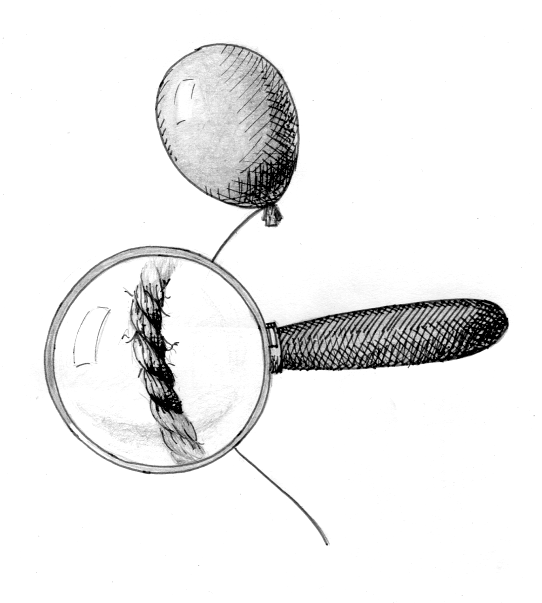
\includegraphics[height=7cm]{abb/echt-3-dim.png}
            \caption{Materielle Körper sind überall echt $3$-dimensional}
            \label{fig:echt-3-dim}
        \end{figure}

        Wie im vorherigen Kapitel werde ich auch hier nicht strikt zwischen Raumregionen und den Objekten, die bestimmte Raumregionen einnehmen, unterscheiden. Mit \glqq Erde\grqq\ ist dann die Raumregion gemeint, die von der Erde eingenommen wird. Analoges gilt für Begriffe wie \glqq Erdoberfläche\grqq , \glqq Küstenlinie\grqq\ u.s.w., die sich auf niederdimensionale Objekte beziehen.
        Niederdimensional heißt im Folgenden immer $0$-, $1$- oder $2$-dimensional.
	
    \section{Niederdimensionale Raumentitäten}\label{sec:niederdimensionale-re}
        Eine Flächenregion ist eine $2$-dimensionale Teilmenge der Oberfläche einer Raumregion -- beispielsweise die obere Seite eines Würfels. 
        \marginpar{Flächenregion,\\Koinzidenz}
        Berühren sich zwei Raumregionen an einer Fläche, so hat jede ihre eigene Flächenregion als Grenze. Nehmen wir beispielsweise zwei aufeinander liegende Würfel, so berühren sich die obere Seite des unteren Würfels und die untere Seite des oberen Würfels, sie werden jedoch nicht als gleich betrachtet. Wir sagen, die beiden Seiten koinzidieren.
        
        Damit wir Flächenregionen als gleich betrachten, müssen sie nicht notwendigerweise die gleichen Raumregionen begrenzen. 
        \marginpar{Gleichheit von Flächenregionen}
        Es genügt, wenn die Raumregionen von denen sie erzeugt werden \glqq von der gleichen Seite kommen\grqq .
        Nehmen wir beispielsweise die Landfläche der Antarktis. Wir könnten sie als Teil der Erdoberfläche sehen oder als Teil der Oberfläche der Antarktischen Platte. In beiden Fällen kommen die erzeugenden Raumregionen \glqq von unten\grqq . Somit sind die beiden Flächenregionen gleich.
    
        Koinzidenz ist eine Äquivalenzrelation auf den niederdimensionalen Raumentitäten, d.h. insbesondere, dass eine Flächenregion immer mit sich selbst koinzidiert. 
        \marginpar{euklidische Fläche}
        Die Äquivalenzklassen der Koinzidenz auf den Flächenregionen werde ich im Weiteren \glqq euklidische Flächen\grqq\ nennen. 
        Während eine euklidische Fläche lediglich durch die Punkte charakterisiert wird, die sie im einbettenden Raum einnimmt, \glqq weiß\grqq\ die Flächenregion, von welcher Seite die Raumregion kommt, die durch sie begrenzt wird.

        Welche Teilmengen des einbettenden Raumes als euklidische Flächen gelten, hängt unter anderem davon ab, welche Mengen als Raumregionen zugelassen sind. Insbesondere wollen wir sicherstellen, dass die gesamte Oberfläche einer beliebigen Raumregion eine Flächenregion ist. Daraus ergibt sich als weitere Bedingung, dass Raumregionen überall einen $2$-dimensionalen Rand haben sollen. Dies verbietet insbesondere niederdimensionale Löcher in Raumregionen. Die Erde ohne ihren Mittelpunkt beispielsweise wäre keine Raumregion, da bei diesem Körper der Mittelpunkt ein Randpunkt wäre und die Oberfläche somit an dieser Stelle $0$-dimensional.
    
        Zwei Flächenregionen überlappen, wenn ihre euklidischen Flächen gemeinsame $2$-dimensionale Teile haben und diese gemeinsamen Teile wiederum Teile haben, die Raumregionen begrenzen, die von der gleichen Seite kommen (siehe Abbildung \ref{fig:overlap}).
        \marginpar{Überlappung}
    
%         \todo[inline]{Bilder zu overlap zusammenfassen}
%         
        \begin{figure}[ht]
            \centering
            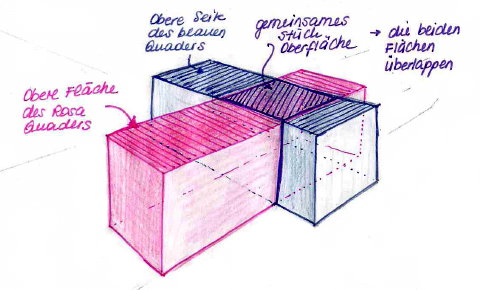
\includegraphics[height=5cm]{abb/overlap.png}
            \caption{Zwei Flächen, die überlappen}
            \label{fig:overlap}
        \end{figure}
        
        \begin{figure}[ht]
            \centering
            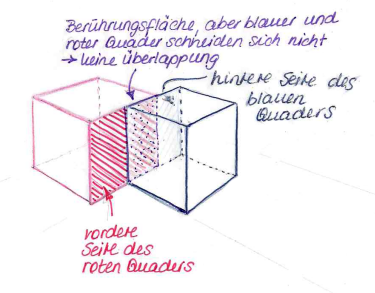
\includegraphics[height=5cm]{abb/no-overlap.png}
            \caption{Zwei Flächen, die koinzidierende Teile haben, aber nicht überlappen}
            \label{fig:no-overlap}
        \end{figure}

    %\subsubsection{Von Flächenregionen zu Linienregionen}
        Analog zur Konstruktion von Flächenregionen und euklidischen Flächen aus Raumregionen können wir aus Flächenregionen Linienregionen und euklidische Linien erzeugen. 
        \marginpar{Linienregion,\\euklidische Linie}
        Eine Linienregion ist eine $1$-dimensionale Teilmenge des Randes einer Flächenregion und eine euklidische Linie ist die Menge der Punkte im einbettenden Raum, die dieser Linienregion entspricht und dabei die dahinter liegenden Raum- und Flächenregionen vergisst.
        Ob zwei Linienregionen gleich sind oder lediglich koinzidieren hängt nun von den zugrundeliegenden Flächenregionen ab und diese wiederum von den dahinter liegenden Raumregionen.

    %\subsubsection{Von Linienregionen zu Punktregionen}
        Auf gleiche Weise entstehen Punktregionen und euklidische Punktmengen aus Linienregionen. 
        \marginpar{Punktregion,\\euklidische Punktmenge}
        Zwei Punktregionen können nur gleich sein, wenn die Linienregionen, durch die sie erzeugt werden, ein gewisses Stück weit gleich aussehen, also überlappen.

        Raumregionen, euklidische Flächen, Linien und Punktmengen werden euklidische Entitäten genannt.
        \marginpar{(niederdimensionale) euklidische Entität}
        Die letzten drei heißen niederdimensionale euklidische Entitäten.

    %\section{Eigenschaften ordinärer Raumentitäten (Zusammenfassung)}\label{sec:zusammenfassung}
    \section{Eigenschaften ordinärer Raumentitäten}\label{sec:zusammenfassung}
        Der hier vorgestellte Interpretationsansatz baut auf den Eigenschaften der ordinären Raumentitäten auf, die ich im Folgenden deshalb zusammenfasse.

        \paragraph{Eigenschaften von Raumregionen:} 
        \begin{itemize}
            \item[(R0)] Raumregionen sind beschränkt.
            \item[(R1)] Sie sind überall echt $3$-dimensional, insbesondere enthalten sie keine niederdimensionalen Ausläufer.
            \item[(R2)] Ihr Rand ist überall echt $2$-dimensional.
            \item[(R3)] Sie enthalten keine niederdimensionalen Löcher.
        \end{itemize}
        
        \paragraph{Eigenschaften von euklidischen Flächen:} 
        \begin{itemize}
            \item[(F0)] Euklidische Flächen liegen auf dem Rand von Raumregionen.
            \item[(F1)] Sie sind überall echt $2$-dimensional, insbesondere enthalten sie keine $1$- oder $0$-dimensionalen Ausläufer oder $3$-dimensionalen Klumpen.
            \item[(F2)] Ihr Rand ist überall echt $1$-dimensional.
            \item[(F3)] Sie enthalten sie keine $1$- oder $0$-dimensionalen Löcher.
        \end{itemize}
            
        \paragraph{Eigenschaften von Flächenregionen:}
        \begin{itemize}
            \item[(F4)] Flächenregionen begrenzen Raumregionen.
            \item[(F5)] Zu jeder Flächenregion gehört genau
%\todo[inline]{\small FL-Absicherung 03.05.: ``genau'' i.O.? Analog für nachfolgende *-regionen ... -> BH: i.O.}
                        eine euklidische Fläche.
            \item[(F6)] Eine Flächenregion ist die ihr zugehörige euklidische Fläche, zusammen mit der Information, welche Raumregionen durch sie begrenzt werden.
            \item[(F7)] Verschiedene Raumregionen, die durch die gleiche Flächenregion begrenzt werden, kommen an jedem Punkt der zugehörigen euklidischen Fläche aus derselben Richtung.
        \end{itemize}

        \paragraph{Eigenschaften von euklidischen Linien:} 
        \begin{itemize}%[Eigenschaften von Linien]
            \item[(L0)] Euklidische Linien liegen auf dem Rand von euklidischen Flächen.
            \item[(L1)] Sie sind überall echt $1$-dimensional, insbesondere enthalten sie keine isolierten Punkte.
            \item[(L2)] Ihr Rand ist überall echt $0$-dimensional.
            \item[(L3)] Sie enthalten sie keine $0$-dimensionalen Löcher.
        \end{itemize}
            
        \paragraph{Eigenschaften von Linienregionen:}
        \begin{itemize}
            \item[(F4)] Linienregionen begrenzen Flächenregionen.
            \item[(F5)] Zu jeder Linienregion gehört genau eine euklidische Linie.
            \item[(F6)] Eine Linienregion ist die ihr zugehörige euklidische Linie, zusammen mit der Information, welche Flächenregionen durch sie begrenzt werden.
            \item[(F7)] Verschiedene Flächenregionen, die durch die gleiche Linienregion begrenzt werden, kommen an jedem Punkt der zugehörigen euklidischen Fläche aus derselben Richtung.
        \end{itemize}
            
        \paragraph{Eigenschaften von euklidischen Punktmengen:} 
        \begin{itemize}%[Eigenschaften von Punktmengen]
            \item[(P0)] Euklidische Punktmengen liegen auf dem Rand von euklidischen Linien.
        \end{itemize}
        
        \paragraph{Eigenschaften von Punktregionen:}
        \begin{itemize}
            \item[(F4)] Punktregionen begrenzen Linienregionen.
            \item[(F5)] Zu jeder Punktregion gehört genau eine euklidische Punktmenge.
            \item[(F6)] Eine Punktregion ist die ihr zugehörige euklidische Punktmenge, zusammen mit der Information welche Linienregionen durch sie begrenzt werden.
            \item[(F7)] Verschiedene Linienregionen, die durch die gleiche Punktregion begrenzt werden, kommen an jedem Punkt der zugehörigen euklidischen Punktmenge aus derselben Richtung.
        \end{itemize}

% 	
% 	\paragraph{Gleichheit von ordinären Raumentitäten} 
% 	\begin{itemize}%[Gleichheit von ordinären Raumentitäten]
% 		\item[(G3)] Zwei Raumregionen sind gleich, wenn sie die gleichen Punkte des einbettenden Raumes einnehmen.
% 		\item[(G2)] Zwei Flächenregionen sind gleich, wenn ihre zugehörigen euklidischen Flächen gleich sind und die Raumregionen, die durch sie begrenzt werden überall von der gleichen Seite kommen.
% 		\item[(G1)] Zwei Linienregionen sind gleich, wenn ihre zugehörigen euklidischen Linien gleich sind und \textcolor{red}{sie eine Umgebung haben, in der die Grenzflächen, die durch sie begrenzt werden, gleich aussehen}.
% 		\item[(G0)] Zwei Grenzpunktmengen sind gleich, wenn sie die gleichen Punkte im umgebenden Raum einnehmen und die Grenzlinien, durch die sie erzeugt werden gemeinsame Stücke haben in der Nähe der Punkte.
% 	\end{itemize}
% 	
% 	\paragraph{Koinzidenz} 
% 	\begin{itemize}
% 	    \item[(K0)] Zwei Punktregionen koinzidieren, wenn ihre zugehörigen euklidischen Punktmengen gleich sind.
%         \item[(K1)] Zwei Linienregionen koinzidieren, wenn ihre zugehörigen euklidischen Linien gleich sind.
%         \item[(K2)] Zwei Flächenregionen koinzidieren, wenn ihre zugehörigen euklidischen Flächen gleich sind.
% 		\item[(K3)] Zwei Raumregionen können nicht koinzidieren.
% 	\end{itemize}

	\paragraph{Koinzidenz} 
	\begin{itemize}
	    \item[(K0)] Zwei niederdimensionale Raumentitäten koinzidieren, wenn die ihnen zugehörigen euklidischen Entitäten gleich sind.
	\end{itemize}

	
%\subsection{Repräsentanten und Objektäquivalenz}
    \section{Das Universum der \strukt}\label{sec:universum}

        Eine Flächenregion begrenzt unendlich viele Raumregionen.
        Kennen wir jedoch eine Raumregion, die von einer bestimmten Flächenregion $u$ begrenzt wird, so wissen wir, dass jede andere Raumregion, die an jedem Punkt der zugehörigen euklidischen Fläche von der gleichen Seite kommt, auch von $u$ begrenzt wird.
        Raumregionen hingegen, für die das nicht der Fall ist, werden nicht von $u$ begrenzt (siehe Abbildung \ref{fig:sb}).
%         Betrachte als Beispiel Abbildung \ref{fig:sb}. 
%         Dort gilt:
%         Wenn $x$ durch $u$ begrenzt wird, dann auch $y$, nicht jedoch $z$.
%
        \begin{figure}[ht]
            \centering
            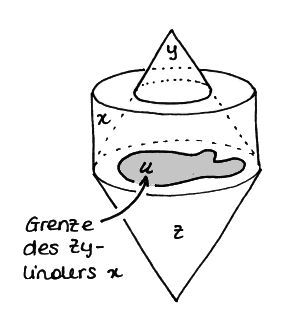
\includegraphics[height=7cm]{abb/sb.png}
            \caption[Räumliche Grenzen]{Räumliche Grenzen: Wenn die Flächenregion $u$ die Raumregion $x$ begrenzt, so auch die $y$, nicht jedoch $z$}
            \label{fig:sb}
        \end{figure}
%
        Um eine Flächenregion zu kennen, genügt es also, die ihr zugehörige euklidische Fläche und eine Raumregion zu kennen, die von ihr begrenzt wird.
        Jedes Paar $(A,B)$ aus einer Raumregion $A$ und einer euklidischen Fläche $B$ auf dem Rand von $A$ repräsentiert also eine Flächenregion.

        Ähnlich, aber komplizierter, verhält es sich bei Linienregionen. 
        Um eine Linienregion zu kennen, müssen wir die ihr zugehörige euklidische Linie und eine Flächenregion kennen, die von ihr begrenzt wird. 
        Da Flächenregionen durch Paare repräsentiert werden, braucht es also Tripel, um Linienregionen zu repräsentieren.
        Zwei Linienregionen zu den gleichen euklidischen Linien und Flächen, die durch die Tripel $(A_1, B, C)$ und $(A_2, B, C)$ repräsentiert werden, können verschieden sein, wenn $A_1$ und $A_2$ von verschiedenen Seiten auf $B$ zukommen. 
        Eine ähnliche Situation ist in Abbildung \ref{fig:objektaeq-linien} dargestellt (Beispiel 1).
%
        \begin{figure}[ht]
            \centering
            \includegraphics[height=5cm]{abb/objektaeq-linien.png}
            \caption{Beispiele für äquivalente (2) und nicht äquivalente (1) Linienregionen}
            \label{fig:objektaeq-linien}
        \end{figure}
%        
        Auf dieser Idee -- dass niederdimensionale Raumentitäten durch Tupel repräsentiert werden -- beruht die \strukt, wobei das Symbol $\rep$ für \glqq repräsentantenbasiert\grqq\ steht.
        Zusammengefasst werden in der folgenden Definition Flächen-, Linien- und Punktrepräsentanten definiert und in Abbildung \ref{fig:repr} verdeutlicht.
%
        \begin{dfn}[Repräsentanten]\ \vspace{0pt}
            \begin{enumerate}
                \item Ein \spacedlowsmallcaps{Flächenrepräsentant} ist ein Paar $(A,B)$, 
                    bestehend aus einer Raumregion $A$ und einer euklidischen Fläche $B$ auf deren Rand.\\
                    Die \spacedlowsmallcaps{Menge der Flächenrepräsentanten} bezeichnen wir mit $\rep^2$.
                \item Ein \spacedlowsmallcaps{Linienrepräsentant} ist ein Tripel $(A,B,C)$, 
                    wobei $(A,B)$ ein Flächenrepräsentant ist und $C$ eine euklidische Linie auf dem Rand von $B$.\\
                    Die \spacedlowsmallcaps{Menge der Linienrepräsentanten} bezeichnen wir mit $\rep^1$.
                \item Ein \spacedlowsmallcaps{Punktrepräsentant} ist ein Quadrupel $(A,B,C,D)$, 
                    wobei $(A,B,C)$ ein Linienrepräsentant ist und $D$ eine euklidische Punktmenge auf dem Rand von $B$.\\
                    Die \spacedlowsmallcaps{Menge der Punktrepräsentanten} bezeichnen wir mit $\rep^0$.
            \end{enumerate}
        \end{dfn}
%
        \begin{figure}[ht]
            \centering
            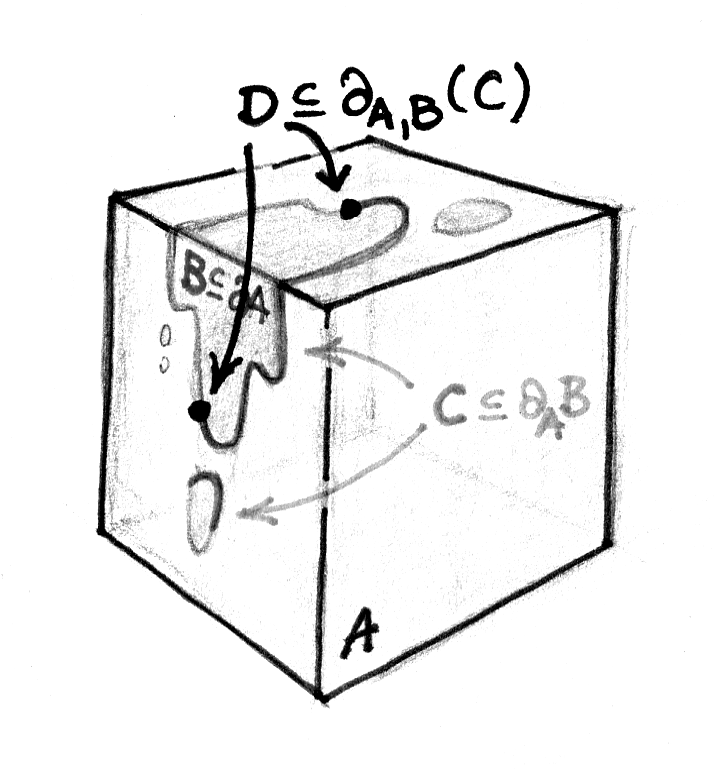
\includegraphics[height=5cm]{abb/repr.png}
            \caption[Grundbegriffe der $\mathcal{R}$-Struktur]{Grundbegriffe der \strukt:\\
                    $A$ ist eine Raumregion, $B$ eine euklidische Fläche, $C$ eine euklidische Linie und $D$ eine euklidische Punktmenge. $(A,B)$ ist ein Flächenrepräsentant, $(A,B,C)$ ein Linienrepräsentant und $(A,B,C,D)$ ein Punktrepräsentant.}
            \label{fig:repr}
        \end{figure}
%
        Eine Äquivalenzrelation auf der Menge der Repräsentanten, für die zwei Repräsentanten äquivalent sind, wenn sie die gleiche Raumentität repräsentieren, heißt Objektäquivalenz.
        \marginpar{Objektäquivalenz}
        Eine Objektäquivalenz erfasst also in geeigneter Weise, was es heißt, dass zwei Raumentitäten \glqq von der gleichen Seite\grqq\ oder \glqq aus der gleichen Richtung\grqq\ kommen.
        Niederdimensionale Raumentitäten lassen sich also als Äquivalenzklassen einer Objektäquivalenz auffassen, was in folgender Definition präzisiert wird.
%
        \begin{dfn}[Flächen-, Linien- und Punktregionen]\ \vspace{8pt}

            \noindent
            Sei $\sim$ eine Objektäquivalenz.
            %
            \begin{enumerate}
        %			
                \item Für $(A,B) \in \rep^2$ bezeichnet 
                    \begin{align*}
                        [A,B] := \{(A',B') \in \rep^2 \mid (A',B') \sim (A,B)\}
                    \end{align*}
                    die Äquivalenzklasse von $(A,B)$ bezüglich der Objektäquivalenz.\\
                    Diese Äquivalenzklassen heißen \spacedlowsmallcaps{Flächenregionen}.
                    
                \item Für $(A,B,C) \in \rep^1$ bezeichnet
                    \begin{align*}
                        [A,B,C] := \{(A',B',C') \in \rep^1 \mid (A',B',C') \sim (A,B,C)\}
                    \end{align*}			 
                    die Äquivalenzklasse von $(A,B,C)$ bezüglich der Objektäquivalenz.\\
                    Diese Äquivalenzklassen heißen \spacedlowsmallcaps{Linienregionen}.
        %			
                \item Für $(A,B,C,D) \in \rep^0$ bezeichnet
                    \begin{align*}
                        &[A,B,C,D] := \\
                        &\{(A',B',C',D') \in \rep^0 \mid (A',B',C',D') \sim (A,B,C,D)\}
                    \end{align*}			 
                    die Äquivalenzklasse von $(A,B,C,D)$ bezüglich der Objektäquivalenz.\\
                    Diese Äquivalenzklassen heißen \spacedlowsmallcaps{Punktregionen}.
        %			
            \end{enumerate}
            %
            \noindent	
                Für $i \in \{0,1,2\}$ ist $\univ^i := \rep^i /_\sim$ die \spacedlowsmallcaps{Menge der Äquivalenzklassen} von $\rep^i$.\\
                $\univ^3$ ist die \spacedlowsmallcaps{Menge der Raumregionen}.
                
        \end{dfn}
%        
        In Abbildung \ref{fig:objektaeq-flaechen} sind Beispiele für äquivalente und nicht äquivaleten Flächenregionen dargestellt.
%
        \begin{figure}[ht]
            \centering
            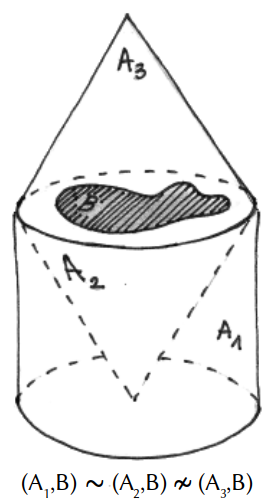
\includegraphics[height=7cm]{abb/objektaeq-flaechen.png}
            \caption{Beispiele für äquivalente und nicht äquivalente Flächenrepräsentanten}
            \label{fig:objektaeq-flaechen}
        \end{figure}
%
        Damit können wir das Universum der \strukt definieren, das aus den Raum-, Flächen-, Linien- und Punktregionen besteht.
%
        \begin{dfn}[Universum]\ \vspace{8pt}

            \noindent
            Das Universum der \strukt ist definiert als
            \begin{align*}
                \univ = \univ^3 \cup \univ^2 \cup \univ^1 \cup \univ^0
            \end{align*}
                    
        \end{dfn}
%        
        Da $\univ^3$, $\univ^2$, $\univ^1$ und $\univ^0$ paarweise disjunkt sind, lässt sich die folgende Funktion auf $U$ definieren:
%    
        \begin{dfn}[Dimensionsfunktion]\ \\
            $\Gdim : \univ \to \N$ ist definiert durch
            $$ \Gdim(x) = i \quad \Leftrightarrow \quad x \in \univ^i $$
        \end{dfn}



    \section{Primitive Relationen}\label{sec:prim-rel-1}

        Die Interpretation der primitiven Relationen in $\theoryBSO$ unter der \strukt kann vollständig auf die gewählte Objektäquivalenz zurückgeführt werden, die im Folgenden mit $\sim$ bezeichnet wird.
        %Zur Unterscheidung werden die Symbole der Struktur mit einem hochgestellten $\strukt$ versehen.

        Die
        \marginpar{$\GSReg$}
        Interpretation des Symbols $\GSReg$ als Menge der Raumregionen ist selbsterklärend.
        
        Für
        \marginpar{$\Gsb$}
        die Interpretation des Symbols $\Gsb$ rufen wir uns ins Gedächtnis:
        Eine Flächenregion, die durch einen Flächenrepräsentanten $(A_1,B)$ repräsentiert wird, begrenzt eine Raumregion $A_2$, wenn $A_1$ und $A_2$ überall auf der gleichen Seite von $B$ liegen. In diesem Fall sind dann $(A_1,B)$ und $(A_2, B)$ äquivalent.
        Diese Überlegung lässt sich auf andere Dimensionen erweitern und führt zu folgender Definition:
%
        \begin{dfn}[Die $\Gsb$-Relation in der \strukt]\ \vspace{0pt}

            \begin{enumerate}
                \item Für $(A_1,B_1) \in \rep^2$, $A_2 \in \univ^3$ gilt 
                    \begin{align*}
                        \Gsb([A_1,B_1],A_2) \quad \Leftrightarrow \quad (A_1,B_1) \sim (A_2,B_1)
                    \end{align*}
                \item Für $(A_1,B_1,C_1) \in \rep^1$, $(A_2,B_2) \in \rep^2$ gilt 
                    \begin{align*}
                        &\Gsb([A_1,B_1,C_1],[A_2,B_2]) \quad \\
                        &\Leftrightarrow  \quad (A_1,B_1,C_1) \sim (A_2,B_2,C_1)
                    \end{align*}
                \item Für $(A_1,B_1,C_1,D_1) \in \rep^0$, $(A_2,B_2,C_2) \in \rep^1$ gilt 
                    \begin{align*}
                        &\Gsb([A_1,B_1,C_1,D_1],[A_2,B_2,C_2]) \quad \\
                        &\Leftrightarrow  \quad (A_1,B_1,C_1,D_1) \sim (A_2,B_2,C_2,D_1)
                    \end{align*}
                %\item Für $x \in \U^i$, $y \in \U^j$ mit $i+1 \neq j$ gilt $\neg sb(x,y)$
                \item Für $x, y$ mit $\Gdim(x) + 1 \neq \Gdim(y)$ gilt $\neg \Gsb(x,y)$
            \end{enumerate}
            
        \end{dfn}
%        
        Als direkte Folgerung aus dieser Definition ergibt sich folgender Satz
%        
        \begin{satz}\label{satz:sb-einfacher-fall}\ \vspace{0pt}
            
            \begin{itemize}
                \item Für alle Flächenrepräsentanten $(A,B) \in \rep^2$ gilt: \\$\Gsb([A,B],A)$
                \item Für alle Linienrepräsentanten $(A,B,C) \in \rep^1$ gilt: \\$\Gsb([A,B,C],[A,B])$
                \item Für alle Punktrepräsentanten $(A,B,C,D) \in \rep^0$ gilt: \\$\Gsb([A,B,C,D],[A,B,C])$
            \end{itemize}
        \end{satz}
%    
        Zwei
        \marginpar{$\Gscoinc$}
        niederdimensionale Raumentitäten koinzidieren, wenn die ihnen zugehörigen euklidischen Entitäten gleich sind. Damit ergibt sich als Interpretation für das $\Gscoinc$-Symbol:
%    
        \begin{dfn}[Die $\Gscoinc$-Relation in der \strukt]\ \vspace{0pt}

            \begin{enumerate}
                \item Für $A_1, A_2 \in \univ^3$ gilt: $\neg \Gscoinc(A_1,A_2)$
                \item Für $(A_1,B_1), (A_2,B_2) \in \rep^2$ gilt 
                    \begin{align*}
                        \Gscoinc([A_1,B_1],[A_2,B_2]) \quad \Leftrightarrow  \quad B_1 = B_2
                    \end{align*}
                \item Für $(A_1,B_1,C_1), (A_2,B_2,C_2) \in \rep^1$ gilt 
                    \begin{align*}
                        \Gscoinc([A_1,B_1,C_1],[A_2,B_2,C_2]) \quad \Leftrightarrow  \quad C_1 = C_2
                    \end{align*}
                \item Für $(A_1,B_1,C_1,D_1), (A_2,B_2,C_2,D_2) \in \rep^0$ gilt 
                    \begin{align*}
                        &\Gscoinc([A_1,B_1,C_1,D_1],[A_2,B_2,C_2,D_2]) \\
                        &\Leftrightarrow  \quad D_1 = D_2
                    \end{align*}
                %\item Für $x \in \U^i$, $y \in \U^j$ mit $i \neq j$ gilt $\neg scoinc(x,y)$
                \item Für $x, y$ mit $\Gdim(x) \neq \Gdim(y)$ gilt $\neg \Gscoinc(x,y)$.
            \end{enumerate}
            
        \end{dfn}%
%        
        Aus dieser Definition ergibt sich trivialerweise:
%        
        \begin{satz}\ \\
            Die $\Gscoinc$-Relation ist eine Äquivalenzrelation auf $\univ^2 \cup \univ^1 \cup \univ^0$.
        \end{satz}
%    
        Die
        \marginpar{$\Gspart$}
        Überlegungen zur Interpretation des Symbols $\Gspart$ ähneln den Überlegungen zur Interpretation von $\Gsb$.
    
        Für Raumregionen ist klar: Eine Raumregion ist räumlicher Teil einer anderen, wenn sie eine Teilmenge dieser ist.
    
        Damit eine Flächenregion räumlicher Teil einer anderen ist, muss die ihr zugehörige euklidische Fläche Teil der euklidischen Fläche der anderen sein.
        Dies reicht jedoch nicht, wie Abbildung \ref{fig:spart-flaechen} zeigt.
        
        Seien $(A_1,B_1)$ und $(A_2,B_2)$ Flächenrepräsentanten mit $B_1 \subseteq B_2$. Damit $[A_1,B_1]$ räumlicher Teil von $[A_2,B_2]$ ist, müssen $A_1$ und $A_2$ von der gleichen Seite auf $B_1$ zukommen. Dann ist $(A_1,B_2)$ äquivalent zu $(A_2, B_1)$.
            
        Analoge Bedingungen gelten für die $\Gspart$-Beziehung von Linienregionen. Beispiele hierzu sind in Abbildung \ref{fig:spart-linien} dargestellt.
        Nun können wir definieren:
%
        \begin{dfn}[Die $\Gspart$-Relation in der \strukt]\ \vspace{0pt}

            \begin{enumerate}
                \item Für $A_1, A_2 \in \univ^3$ gilt $\Gspart(A_1,A_2)$ gdw.\ $A_1 \subseteq A_2$
        %		
                \item Für $(A_1,B_1), (A_2,B_2) \in \rep^2$ gilt \\
                $\Gspart([A_1,B_1],[A_2,B_2])$ gdw.\ 
                    \begin{enumerate}
                        \item $B_1 \subseteq B_2$
                        \item $(A_1, B_1) \sim (A_2, B_1)$
                    \end{enumerate}	
        %			
                \item Für $(A_1,B_1,C_1), (A_2,B_2,C_2) \in \rep^1$ gilt \\
                $\Gspart([A_1,B_1,C_1],[A_2,B_2,C_2])$ gdw.\ 
                    \begin{enumerate}
                        \item $C_1 \subseteq C_2$
                        \item $(A_1, B_1, C_1) \sim (A_2, B_2, C_1)$
                    \end{enumerate}	
        %			
                \item Für $(A_1,B_1,C_1,D_1), (A_2,B_2,C_2,D_2) \in \rep^0$ gilt \\
                $\Gspart([A_1,B_1,C_1,D_1],[A_2,B_2,C_2,D_2])$ gdw.\
                    \begin{enumerate}
                        \item $D_1 = D_2$
                        \item $(A_1, B_1, C_1, D_1) \sim (A_2, B_2, C_2, D_1)$
                    \end{enumerate}	
        %			
                \item Für $x, y$ mit $\Gdim(x) \neq \Gdim(y)$ gilt $\neg \Gspart(x,y)$
        %		
            \end{enumerate}
            
        \end{dfn}
%        
        \begin{figure}[ht]
            \centering
            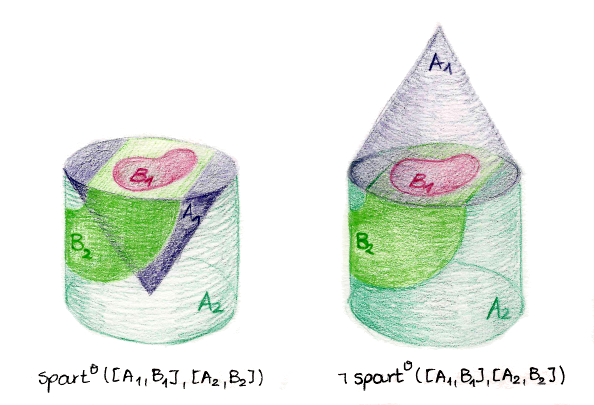
\includegraphics[height=7cm]{abb/spart-flaechen.png}
            \caption{Beispiel und Gegenbeispiel zu $\Gspart$ bei Flächenregionen}
            \label{fig:spart-flaechen}
        \end{figure}
%
        \begin{figure}[ht]
            \centering
            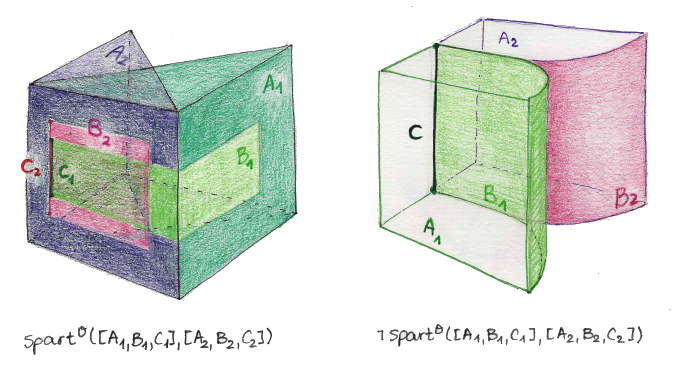
\includegraphics[width=0.9\textwidth]{abb/spart-linien.png}
            \caption{Beispiel und Gegenbeispiel zu $\Gspart$ bei Linienregionen}
            \label{fig:spart-linien}
        \end{figure}
%
    \section{Ausblick}\label{sec:ausblick}
        Der hier skizzierte Interpretationsansatz ist bislang unvollständig.

        Zum
        \marginpar{Grundraum}
        einen ist offen, in welchem Raum die euklidischen Entitäten zu finden sind ($\R^3$ als Vektorraum, affiner Raum, ... ).
        In dieser Arbeit habe ich mich für den $\R^3$ als mit der euklidischen Metrik ausgestatten metrischen Raum entschieden. 
        Dieser wird in Kapitel \ref{chap:topologie-grundlagen} eingeführt.

        Welche
        \marginpar{euklidische Entitäten}
        Teilmengen dieses Raumes die gewünschten Eigenschaften von euklidischen Entitäten aufweisen, ist eine anspruchsvolle Frage, die im Rahmen dieser Arbeit nicht erschöpfend untersucht werden kann.
        Ich nutze hier die einfachen Mengen, die in Kapitel \ref{chap:topologie-erweiterung} eingeführt werden.
        Sie schließen einige offensichtlich unerwünschte Fälle aus.

        Zu
        \marginpar{Randbegriff}
        dieser Frage gehört auch, was als Rand der euklidischen Entitäten zählt, auf dem dann die nächst-niedriger-dimensionalen Entitäten zu finden sind.
        Dafür wird ebenfalls in Kapitel \ref{chap:topologie-erweiterung} der sogenannte äußere Rand eingeführt.

        Schließlich
        \marginpar{Objektäquivalenz}
        muss noch eine Objektäquivalenz definiert werden, die in geeigneter Weise erfasst, was es heißt, wenn zwei Raumentitäten \glqq von der gleichen Seite\grqq\ auf eine dritte zukommen.
        Mit ihrer Einführung in Kapitel \ref{chap:bso-struktur} werden die letzten Lücken in der Definition der \strukt geschlossen.

% 
% \part{Die topologische Seite}
% 
% \chapter{Grundlagen der Topologie}\label{chap:topologie-grundlagen}

Die in der vorliegenden Arbeit angegebenen Strukturen bauen auf topologischen Begriffen auf.
Die Abschnitte \ref{sec:allg-top-raeume} (Allgemeine topologische Räume), \ref{sec:teilraum-top} (Teilraumtopologie) und \ref{sec:top-metr-raeume} (Metrische Räume) führen Grundbegriffe der Topologie ein, wie sie auch in der Literatur zu finden sind. Sie dienen in erster Linie dazu die hier verwendeten Notationen einzuführen enthalten aber auch einige Sätze und Beweise.

Die eingeführten Begriffe und Notationen finden sich auf den herausnehmbaren Übersichtsblättern (Übersicht 4).

%%% Allgemeine topologische Räume %%%%%%%%%%%%%%%%%%%%%%%%%%%%%%%%%%%%%%%%%%%%%%%%%%%%%%%


\section{Allgemeine topologische Räume}\label{sec:allg-top-raeume} 
    %
    In diesem Abschnitt werden grundlegende Begriffe der Topologie eingeführt sowie einige relevante Sätze vorgestellt. 
    Für ein tieferes Verständnis sei auf die Literatur verwiesen ([\cite{jaenich-k-2013--a}] oder [\cite{manetti-m-2015--a}]). 
    Für mich geht es hier vor allem darum, eigene Notationen einzuführen, da sich die Standardnotationen schnell als unpraktisch erweisen, wenn es nötig wird mit verschiedenen topologischen Räumen gleichzeitig zu arbeiten.
    
    Der
    %\marginpar{Topologischer Raum,\\Topologie,\\offene Menge}
    \marginpar{Topologischer Raum}
    grundlegendste Begriff hierbei ist natürlich der des topologischen Raumes.
    Das ist eine Menge, von der wir wissen, welche ihrer Teilmengen offen sind.
    \begin{dfn}[Topologischer Raum, Topologie, offene Menge]\label{def:top} \ \\
        Ein \thmemph{topologischer Raum} ist ein Paar $(X,\offen)$ bestehend aus
    %
        \begin{itemize}
            \item einer Menge $X$ (\thmemph{Grundmenge}) 
            \item einer Menge $\offen \subseteq 2^X$ von Teilmengen von $X$ (\thmemph{Topologie})
        \end{itemize}
    %
        mit folgenden Eigenschaften:
    %
        \begin{enumerate}
            \item[T1] $\varnothing, X \in \offen$ %($\O$ und $X$ sind offen) 
            \item[T2] $A,B \in \offen \quad \quad \Leftrightarrow \quad \quad A \cap B \in \offen$ %(und damit: endliche Schnitte offener Mengen sind offen)
            \item[T3] $\mathcal{A} \subseteq \offen \quad \quad \Rightarrow \quad \quad \bigcup\limits_{A \in \mathcal{A}} A \in \offen$ %(Beliebige Vereinigungen offener Mengen sind offen).
        \end{enumerate}
    %	
        Wenn $A \in \offen$ ist, so sagen wir: $A$ ist \thmemph{offen} in $(X, \offen)$.
    %
    \end{dfn}
    %
    \begin{konv}\label{konv:top}
        Wenn wir schreiben \glqq Sei $X$ ein topologischer Raum\grqq , so ist der topologische Raum $(X, \offen_X)$ mit $X$ als Grundmenge und zugehöriger Topologie $\offen_X$ gemeint. Wenn keine Verwechslungsgefahr besteht, schreiben wir auch $\offen$ für $\offen_X$.
    \end{konv}
    %
    Aus
    \marginpar{Standardtopologie auf $\R$}
    der Schule ist für die reellen Zahlen der Begriff des offenen Intervalls bekannt. Diese bilden für sich genommen jedoch noch keine Topologie, da Vereinigungen offener Intervalle, die sich nicht überschneiden, keine offene Intervalle sind.
    Durch Abschlussbildung unter Vereinigung lässt sich jedoch mit ihrer Hilfe eine Topologie definieren, die sogenannte Standardtopologie auf $\R$.
    %
    \begin{bsp}[Standardtopologie auf $\R$]\label{bsp:standard-r}\ \\
        Auf $\R$ ist die Standardtopologie folgendermaßen definiert:\\
        Eine Menge $M \subseteq \R$ ist offen, wenn sie leer ist oder sich als Vereinigung offener Intervalle schreiben lässt.
    \end{bsp}
    In Abschnitt \ref{sec:top-metr-raeume} werden wir sehen, dass sich diese Topologie auch aus der Standardmetrik auf $\R$ ergibt.

    Eine
%     \marginpar{offene Umgebung,\\$\offen_X(p)$}
    \marginpar{offene Umgebung}
    offene Umgebung eines Punktes ist eine offene Menge, die ihn enthält.
    \begin{dfn}[Offene Umgebung, $\offen_X(p)$]\label{def:umg} \ \\
        Sei $X$ ein topologischer Raum. Eine Menge $U \subseteq X$ heißt \thmemph{offene Umgebung} von $p$ in $X$, wenn $p \in U \in \offen_X$ gilt. Die \thmemph{Menge der offenen Umgebungen} von $p$ in $X$ notieren wir mit $\offen_X(p)$. Falls wir nur eine Topologie betrachten, schreiben wir auch $\offen(p)$ für $\offen_X(p)$.
    \end{dfn}
%
    Abgeschlossene
%     \marginpar{abgeschlossene Menge,\\$\abg_X$}
    \marginpar{abgeschlossene Menge}
    Mengen sind Komplemente offener Mengen.
    \begin{dfn}[Abgeschlossene Menge, $\abg_X$] \label{def:CX} \ \\
        Seien $X$ ein topologischer Raum, $A \subseteq X$.
        $A$ heißt \thmemph{abgeschlossen} in $X$, falls $X \setminus A \in \offen_X$ ist.
        Die \thmemph{Menge der abgeschlossenen Mengen} in $X$ bezeichnen wir mit $\abg_X$ bzw. falls keine Verwechslungsgefahr besteht mit $\abg$.
    \end{dfn}
    Analog zur Angabe der offenen Mengen, könnten wir auch die abgeschlossenen Mengen nutzen, um eine Topologie zu charakterisieren. Genauer gesagt: Jedes Mengensystem mit den folgenden Eigenschaften charakterisiert eine Topologie.

    \begin{satz}[Eigenschaften der Menge $\abg$]\label{satz:CX}\ \\
        Sei $X$ ein topologischer Raum. Dann gelten
        \begin{enumerate}
            \item $\varnothing, X \in \abg$ 
            \item $A,B \in \abg \quad \quad \Rightarrow \quad \quad  A \cup B \in \abg$ 
            \item $\mathcal{A} \subseteq \abg \quad \quad \Rightarrow \quad \quad \bigcap\limits_{A \in \mathcal{A}} A \in \abg$ 
        \end{enumerate}
        (Beweis trivial)
    \end{satz}
%     (Beweis trivial)
%    
    Folgender Satz ist eine einfache Folgerung aus den Definitionen.
    \begin{satz}\label{satz:differenz}%verwendung: satz:rand-abg
        Sei $X$ ein topologischer Raum, $A\in \abg$ und $B \in \offen$. Dann gelten:
        \begin{enumerate}
            \item $A \setminus B \in \abg$
            \item $B \setminus A \in \offen$
        \end{enumerate}    
    \end{satz}
%    
    \begin{bew}
        Mit $A \in \abg$ ist $X\setminus A \in \offen$ und somit gelten
        \begin{enumerate}
            \item $X \setminus (A \setminus B) = (X \setminus A) \cup (X \cap B) \in \offen$.
            \item $B \setminus A = B \cap (X \setminus A) \in \offen$.
        \end{enumerate}
    \end{bew}
%
%
    Ein
%     \marginpar{Randpunkt,\\Randoperator,\\Rand,\\$\rand_X$}
    \marginpar{Rand}
    Randpunkt einer Menge ist ein Punkt, für den in jeder offenen Umgebung sowohl Punkte im Inneren als auch außerhalb der Menge liegen. Der Randoperator ordnet jeder Menge die Menge ihrer Randpunkte zu.
%
    \begin{dfn}[Randoperator] \label{def:rand} \ \\
        Sei $X$ ein topologischer Raum. Dann ist der \thmemph{Randoperator} $\rand_X : 2^X \rightarrow 2^X$ auf $X$ definiert durch:
    %	
        \begin{align*}
            \rand_X(A) := \{&x \in X \mid \forall\: U \in \offen_X(x) :\\ 
            &(\: U \cap A \neq \varnothing \:\land\: U \setminus A \neq \varnothing \:))\}
        \end{align*}
        
    \end{dfn}
%
%
    \begin{konv}
        Statt $\rand_X(A)$ schreiben wir auch $\rand_X A$ und falls keine Verwechslungsgefahr besteht $\rand(A)$ bzw. $\rand A$.
    \end{konv}
%
%
    Folgendes
    \marginpar{Standardbeispiel}
    Beispiel für den Rand einer Menge wird im Laufe der Arbeit immer wieder genutzt, um verschiedene Begriffe und Fälle zu verdeutlichen und 
    %im Abschnitt \ref{sssec:standardbsp} 
    im nächsten Kapitel ausgiebiger untersucht.
    Deshalb nenne ich es Standardbeispiel.
    Dies ist natürlich nicht vergleichbar mit der bereits erwähnten Standardtopologie oder der weiter unten eingeführten Standardmetrik, die auch außerhalb der vorliegenden Arbeit eine Bedeutung haben.
%    
    \begin{bsp}[Standardbeispiel]\label{bsp:standardbsp}\ \\
        Sei $$A := \bigcup_{n \in \N} [2^{-2n}, 2^{-2n+1}]$$ aus dem mit der in Bsp.\ \ref{bsp:standard-r} definierten Standardtopologie versehenen Raum $\R$.
        Dann ist
        \begin{align*}
            \rand A = \{\frac{1}{2^n} \mid n \in \N\} \cup \{0\}
        \end{align*}
    \end{bsp}
    %\todo[inline]{BH: begründen? $\to$ FL: Nein, eigentlich nicht nötig, sondern gut einsehbar.\\
% 		Gestolpert bin ich darüber, dass ich zuerst von $\N$ inkl.\ 0 ausging und 
% 		$A := \bigcup_{n \in \N} [2^{-2n-2}, 2^{-2n-1}]$ vorschlagen wollte;
% 		mit $\N$ ohne 0 müsste es das ergänzte `$-$' im Exponenten der 2.\ Komponente aber lösen.
% 		An $\rand A$ lässt sich letztlich auch ersehen, wie $\N$ hier ausgelegt wird,
% 		daher muss m.E. auch kein Zusatzhinweis sein.
% 		}
%    
    \begin{figure}[ht]
        \centering
        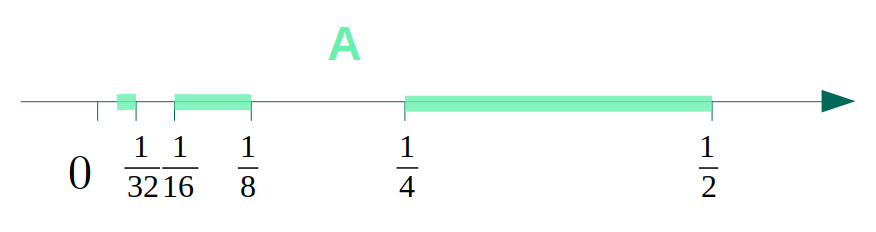
\includegraphics[width=0.6\textwidth]{abb/standardbsp.png}
        \caption{Zum Standardbeispiel}
        \label{fig:standardbsp}
    \end{figure}
%        
    Der
%     \marginpar{Abschlussoperator,\\Abschluss,\\$\abg_X$}
    \marginpar{Abschluss}
    Abschluss einer Menge besteht aus der Menge selbst und all ihren Randpunkten. Diese Punkte liegen in dem Sinne \glqq sehr nah\grqq\ an der Menge, dass sie sich nicht durch offene Umgebungen von der Menge trennen lassen.
%    
    \begin{dfn}[Abschlussoperator, Abschluss]\label{def:abschl} \ \\
        Sei $X$ ein topologischer Raum. Dann ist der \thmemph{Abschlussoperator} $\cl_X : 2^X \rightarrow 2^X$ auf $X$ definiert durch:
    %		
        \begin{align*}
            \cl_X(A) := \{x \in X \mid \forall\: U \in \offen_X(x) : U \cap A \neq \varnothing \}
        \end{align*}
    %	
        $\cl_X(A)$ heißt der \thmemph{Abschluss} von $A$.
    %	
    \end{dfn}
    %
    \begin{konv}
        Statt $\cl_X(A)$ schreiben wir auch $\cl(A)$ wenn klar ist, auf welche Topologie wir uns beziehen.
    \end{konv}
%    
    \begin{bem}[Abschluss einer Menge unter einem Operator]\ \\
        Dem aufmerksamen Leser ist vielleicht aufgefallen, dass der Begriff des Abschlusses einer Menge in dieser Arbeit überladen ist.
        In Beispiel \ref{bsp:standard-r} wurde die Standardtopologie auf $\R$ als Abschluss der Menge der offenen Intervalle unter Vereinigung eingeführt.
        In Abschnitt \ref{sec:offene-fragen} wird die Frage aufgeworfen, ob sich ein Modell für $\theoryBSO$ durch Abschluss unter mereologischer Summenbildung zu einem Modell für $\theoryBS$ erweitern lässt.
        
        Diese beiden Beispiele benutzen den Begriff des Abschlusses einer Menge unter einem Operator. Formal:
        
        Sei $X$ eine Menge und $f: X^n \to X$ ein Operator auf $X$.
        Eine Menge $M \subseteq X$ ist \thmemph{abgeschlossen} unter $f$, falls für alle $m_1, ... , m_n \in M$ gilt: $f(m_1, ... m_n) \in M$.
        Der \thmemph{Abschluss} einer Menge $M$ unter einer Operation $f$ ist die kleinste unter $f$ abgeschlossene Menge, die $M$ enthält.
    \end{bem}
%
%
    Das
    \marginpar{Kern}
    Innere einer Menge besteht aus allen Punkten dieser Menge, die keine Randpunkte sind. Das bedeutet, diese Punkte haben offene Umgebungen, die komplett in der Menge liegen.
%
    \begin{dfn}[Kernoperator, Inneres] \label{def:kern} \ \\
        Sei $X$ ein topologischer Raum. Dann ist der \thmemph{Kernoperator} $\op_X : 2^X \rightarrow 2^X$ auf $X$ definiert durch:
    %	
        \begin{align*}
            \op_X(A) := \{x \in X \mid \exists \, U \in \offen_X(x) : U \subseteq A \}
        \end{align*}
    %	
        $\op_X(A)$ heißt das \thmemph{Innere} oder der \thmemph{Kern} von $A$.

    \end{dfn}
%
    \begin{konv}
        Statt $\op_X(A)$ schreiben wir auch $\op(A)$ wenn klar ist, auf welche Topologie wir uns beziehen.
    \end{konv}
%
    \begin{figure}[ht]
        \centering
        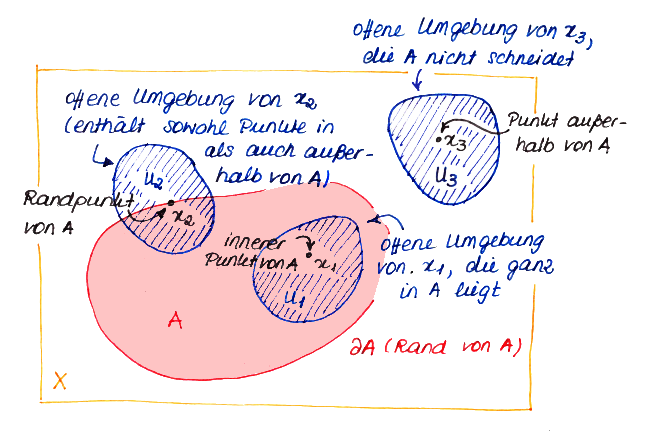
\includegraphics[height=7cm]{abb/top-grundbegr.png}
        \caption{Grundbegriffe der Topologie}
        \label{fig:top-grundbegr}
    \end{figure}
%
%
    \begin{bem}
        Üblicherweise werden der Abschluss von $A$ mit $\bar A$, das Innere mit $A^\circ$ bezeichnet. Da diese Notationen jedoch keine Unterscheidung zwischen verschiedenen Topologien zulassen, sind sie für die vorliegende Arbeit unpraktisch.
    \end{bem}
%    
    \begin{bsp}[Abschluss und Kern am Standardbeispiel]\label{bsp:standardbsp-abschl-kern}\ \\
        Für die in Bsp.\ \ref{bsp:standardbsp} definierte Menge ${A = \bigcup_{n \in \N} [2^{-2n}, 2^{-2n+1}]}$ mit Rand\\${\rand A = \{\frac{1}{2^n} \mid n \in \N\} \cup \{0\}}$ sind Abschluss und Kern gegeben durch:
        \begin{align*}
            \cl(A) &= A \cup \rand A = A \cup \{0\}\\
            \op(A) &= A \setminus \rand A = \bigcup_{n \in \N} (2^{-2n}, 2^{-2n+1})
        \end{align*}
    \end{bsp}
%    \todo[inline]{BH: beweisen? $\to$ FL: Nein, danke, hinreichend einsehbar.\\
%		NB: Da ich hier erneut den Exponenten der 2.\ Komponente angepasst habe, wäre
%		ggf.\ die Arbeit nochmal an anderen Stellen des Standardbeispiels anzuschauen,
%		ob der Exponent auftritt.}
%
    Im
    \marginpar{Eigenschaften\\ von $\cl$, $\op$ und $\rand$}
    Folgenden werden hilfreiche Eigenschaften der topologischen Operatoren aufgeführt, die für die Beweise über die \strukt nützlich sind oder sein könnten.
    \begin{satz}[Eigenschaften des Abschlussoperators] \label{satz:cl}\ \\
        Sei $X$ ein topologischer Raum, $A, B \subseteq X$. Dann gelten
    %	
        \begin{enumerate}
            \item \label{satz:cl.1} $\cl(A)$ ist die kleinste in $X$ abgeschlossene Obermenge von $A$.
            \item \label{satz:cl.2} $\cl(A) = A \cup \rand(A)$.
            \item \label{satz:cl.3} $\cl(A \cap B) \subseteq \cl(A) \cap \cl(B)$
            \item \label{satz:cl.4} $\cl(A \cup B) = \cl(A) \cup \cl(B)$.
            \item \label{satz:cl.5} $\cl(X \setminus A) = X \setminus \op(A)$. 
            \item \label{satz:cl.6} $\cl(A \setminus B) \subseteq \cl(A) \setminus \op(B)$. 
            \item \label{satz:cl.7} $\cl(A) \setminus \cl(B) \subseteq \cl(A \setminus B)$
            \item \label{satz:cl.8} $A \subseteq B \quad \quad \Rightarrow \quad \quad \cl(A) \subseteq \cl(B)$ 
        \end{enumerate}	
        
    \end{satz}
%
    \begin{bew}%[Satz \ref{satz:cl}]
        \ 

        \noindent
        \thmemph{Zu \ref{satz:cl.1}:}
        Seien
        \begin{align} \label{mac}
            \mathcal{M}_A^C &:= \{ U \in \offen \mid U \cap A = \varnothing\} \\
            U_A^C &:= \bigcup\limits_{U \in \mathcal{M}_A^C} U
        \end{align}
        Dann ist $U_A^C$ als Vereinigung offener Mengen wieder offen und es gilt 
        \begin{align}
            \cl(A) = X \setminus U_A^C
        \end{align}
        (Beweis siehe Anhang \ref{anh:cl.1})\\
        Somit ist $\cl(A)$ als Komplement einer offenen Menge abgeschlossen. 
        Es bleibt noch zu zeigen, dass
        \begin{enumerate}
            \item $\cl(A)$ eine Obermenge von $A$ ist und
            \item es keine kleinere in $X$ abgeschlossene Menge gibt, die $A$ enthält.
        \end{enumerate}	 
        Auch diese Beweise sind im Anhang zu finden (ebenfalls \ref{anh:cl.1}).
        \\
            
        \noindent
        \thmemph{Zu \ref{satz:cl.2}-\ref{satz:cl.8}:} siehe \ref{anh:cl.2} - \ref{anh:cl.8}.

    \end{bew}
%
%
    \begin{kor} \label{kor:cl}\ \vspace{0pt}
        \begin{enumerate}
            \item \label{kor:cl.1} $\cl(A)$ ist abgeschlossen in X.
            \item \label{kor:cl.2} $A \subseteq \cl(A)$
            \item \label{kor:cl.3} $A \in \abg \quad \quad \Rightarrow \quad \quad \cl(A) = A$
            \item \label{kor:cl.4} $\cl(\cl(A)) = \cl(A)$
        \end{enumerate}
    \end{kor}
%
    \begin{bew}
        \

        \noindent 
        \thmemph{Zu \ref{kor:cl.1} und \ref{kor:cl.2}:} Offensichtliche Folgerungen aus Satz \ref{satz:cl}.		\ref{satz:cl.1}

        \noindent
        \thmemph{Zu \ref{kor:cl.4}:} Ebenfalls eine Folgerung aus Satz \ref{satz:cl}.\ref{satz:cl.1}. Dieser Satz besagt $\cl(\cl(A))$ ist die kleinste abgeschlossene Obermenge von $\cl(A)$. Da $\cl(A)$ selbst abgeschlossen ist (\ref{kor:cl.1}.) muss also gelten $\cl(\cl(A)) = \cl(A)$.

    \end{bew}
%
%
    \begin{satz}[Eigenschaften des Kernoperators] \label{satz:op}\ \\
        Sei $X$ ein topologischer Raum, $A, B \subseteq X$. Dann gelten:
    %	
        \begin{enumerate}
            \item \label{satz:op.1} $\op(A)$ ist die größte offene Teilmenge von A. %Verwendung: {satz:offeneMengenInAundKompl}
            \item \label{satz:op.2} $\op(A) = A \setminus \rand(A)$.
            \item \label{satz:op.3} $\op(A \cap B) = \op(A) \cap \op(B)$.
            \item \label{satz:op.4} $\op(A) \cup \op(B) \subseteq \op(A \cup B)$
            \item \label{satz:op.5} $\op(X \setminus A) = X \setminus \cl(A)$.
            \item \label{satz:op.6} $\op(A \setminus B) = \op(A) \setminus \cl(B)$. 
            \item \label{satz:op.7} $A \subseteq B \quad \Rightarrow \quad \op(A) \subseteq \op(B)$	
        \end{enumerate}	
        
    \end{satz}
%
    \begin{bew} 
    \ 

    \noindent
    \thmemph{Zu \ref{satz:op.1}:} Sei
        \begin{align}
            \mathcal{M}_A := \{U \in \offen \mid U \subseteq A\}.		
        \end{align}
        Dann gilt 
        \begin{align}
            \op(A) = \bigcup\limits_{U \in \mathcal{M}_A} U
        \end{align}
        (Beweis siehe Anhang \ref{anh:op.1})\\ 
        Dann ist $\op(A)$ als Vereinigung offener Mengen offen und als Vereinigung von Teilmengen von $A$ wieder eine Teilmenge von $A$. Außerdem gilt nach Konstruktion von $\mathcal{M}_A$
        \begin{align}
            \forall\: U \in \offen : U \subseteq A \rightarrow U \subseteq \op(A).
        \end{align}
        Damit ist also $\op(A)$ die größte offene Teilmenge von $A$.
        \\

        \noindent
        \thmemph{Zu \ref{satz:op.2}-\ref{satz:op.6}:} siehe \ref{anh:op.2} - \ref{anh:op.5}	\\

        \noindent
        \thmemph{Zu \ref{satz:op.7}:} Da $\op(A)$ nach \ref{satz:op.1}. offen ist, gibt es für jeden Punkt $x$ in $\op(A)$ eine offene Umgebung, die in $A$ und somit auch in $B$ liegt. Also liegt $x$ auch in $\op(B)$.
        
    \end{bew}
%
%
    \begin{kor} \label{kor:op}\ \vspace{0pt}
        \begin{enumerate}
            \item $\op(A)$ ist offen in $X$. \label{kor:op.1}
            \item $\op(A) \subseteq A$ \label{kor:op.2}
            \item $\op(\op(A)) = \cl(A)$ \label{kor:op.3}
        \end{enumerate}
    %
    \end{kor}
%
    \begin{bew}
        \

        \noindent 
        \thmemph{Zu \ref{kor:op.1} und \ref{kor:op.2}:} Offensichtliche Folgerungen aus Satz \ref{satz:op}.%\ref{satz:op.1}

        \noindent
        \thmemph{Zu \ref{kor:cl.4}:} Ebenfalls eine Folgerung aus Satz \ref{satz:op}.\ref{satz:op.1}. Dieser Satz besagt $\op(\op(A))$ ist die größte in $X$ offene Teilmenge von $op(A)$. Da $op(A)$ selbst offen ist in $X$ (\ref{kor:op.1}.), muss also gelten $\op(\op(A)) = \op(A)$.

    \end{bew}
%    
    Im Allgemeinen gelten nicht ${\cl(A \cap B) = \cl(A) \cap \cl(B)}$ und \\
    ${\op(A \cup B) = \op(A) \cup \op(B)}$, wie folgendes Gegenbeispiel belegt.
    %
    \begin{gegenbsp}
        Wähle ${X := \{1,2\}}$, ${\offen_X := \{\varnothing, \{1\}, \{1,2\}\}}$, ${A:= \{1\}}$ und ${B:=\{2\}}$.
    \end{gegenbsp}
%    
%    
    \begin{satz}[Eigenschaften des Randoperators] \label{satz:rand} \ \\
        Seien $X$ ein topologischer Raum, $A, B \subseteq X$. Dann gelten
    %	
        \begin{enumerate}
            \item \label{satz:rand.1} $\rand(\rand(A)) \subseteq \rand(A)$
            \item \label{satz:rand.2} $\rand(A) = \cl(A) \setminus \op(A)$.
            \item \label{satz:rand.3} $(\rand(A) \cap \op(B)) \cup (\rand(B) \cap \op(A)) \subseteq \rand(A \cap B)$. 
            \item \label{satz:rand.4} $\rand(A \cap B) \subseteq (\rand(A) \cap \cl(B)) \cup (\rand(B) \cap \cl(A))$.
            %\item \label{satz:rand.5} $\rand_X(A \cup B) \subseteq (\rand_X(A) \setminus \op_X(B)) \cup (\rand_X(B) \setminus \op_X(A))$. 
            %\item \label{satz:rand.6} $(\rand_X(A) \setminus \cl_X(B)) \cup (\rand_X(B) \setminus \cl_X(A)) \subseteq \rand_X(A \cup B)$. 
            \item \label{satz:rand.7} $\rand(A \setminus B) \subseteq (\rand(A) \setminus \op(B)) \cup (\rand(B) \cap \cl(A))$. 
            \item \label{satz:rand.8} $\rand(A) = \rand(X \setminus A)$
        \end{enumerate}	
        
    \end{satz}
    %
    Zu den Beweisen von \ref{satz:rand.1} - \ref{satz:rand.7} siehe Anhang \ref{anh:rand.1} - \ref{anh:rand.7}. Der Beweis von \ref{satz:rand.8} ist trivial.
%
%
    \begin{bem} \label{bem:rand}
        Warum ist der Randoperator im Gegensatz zum Abschluss- und zum Kernoperator nicht idempotent? Wieso lässt sich \ref{satz:rand}.\ref{satz:rand.1}. also nicht verschärfen zu $\rand(\rand(A)) = \rand(A)$? Ein einfaches Gegenbeispiel ist nicht schwer zu finden. Seien $X := \{a, b\}$, $\offen := \{\varnothing, X\}$, $A := \{a\}$. Dann lässt sich leicht nachprüfen, dass $\offen$ eine Topologie ist und dass $\rand(A) = X$ und $\rand(\rand(A)) = \varnothing$ gelten.
    \end{bem}
%
%
    \begin{kor}\label{kor:rand-abg}
        Seien $X$ ein topologischer Raum und $A \subseteq X$. Dann gilt $\rand A \in \abg$.
    \end{kor}
    %
    \begin{bew}
        Da $\cl(A) \in \abg$ und $\op(A) \in \offen$, ist wegen \\
        $\rand A = \cl(A) \setminus \op(A)$ nach Satz \ref{satz:differenz} $\rand A \in \abg$.
    \end{bew}
%    
    Der folgende Satz erweist sich als nützlich, wenn wir die Ränder lokal gleicher Mengen betrachten, die in Abschnit \ref{sec:lokale-gleichheit} eingeführt werden und Grundlage der Definition der Objektäquivalenz sind.
%
    \begin{satz} \label{satz:AdB=AdC}\ \vspace{8pt}

        \noindent
        Seien $X$ ein topologischer Raum, $A \in \offen_X$ und $B, C \subseteq X$ mit $A \cap B = A \cap C$. Dann gilt 
    %
        \begin{align*}
            A \cap \rand B = A \cap \rand C.
        \end{align*}
    %	
        (Beweis siehe Anhang \ref{anh:AdB=AdC})
    \end{satz}
    %(Beweis siehe Anhang \ref{anh:AdB=AdC})
%    
%    
    Bei
    \marginpar{Häufungspunkt}
    der Analyse des Standardbeispiels in Abschnitt \ref{ssec:standardbsp} wird der Begriff des Häufungspunktes einer Menge genutzt. 
    Das ist ein Punkt, für den in jeder Umgebung noch weitere Punkte aus der Menge liegen.
%
    \begin{dfn}[Häufungspunkt]\label{def:hp}\ \\
        Seien $X$ ein topologischer Raum, $A \subseteq X$.
        Ein Punkt $x \in X$ heißt \thmemph{Häufungspunkt} von $A$ in $X$, falls gilt
        \begin{align*}
            \forall\: U \in \offen(x) : U \cap (A \setminus \{x\}) \neq \varnothing
        \end{align*}
        $\HP_X(A)$ bezeichnet die \thmemph{Menge der Häufungspunkte} von $A$ in $X$.
        Falls eine Verwechslung ausgeschlossen ist, schreiben wir auch $\HP(A)$ für $\HP_X(A)$.
    \end{dfn}
%
%
    Man beachte, dass eine Menge auch Häufungspunkte haben kann, die außerhalb von ihr liegen, wie folgendes Beispiel zeigt.
%    
    \begin{bsp}[Häufungspunkte am Standardbeispiel]\ \\
        Die sowohl die Menge ${A = \bigcup_{n \in \N} [2^{-2n}, 2^{-2n+1}]}$ aus Bsp.~\ref{bsp:standardbsp} als auch $\R \setminus A$ haben $0$ als Häufungspunkt.
    \end{bsp}
%    
    \begin{bew}
        Dass $0$ Häufungspunkt von $\R \setminus A$ ist, ist klar, denn jede offene Umgebung von $0$ enthält negative Zahlen, die nicht in $A$ liegen.\\
        Sei nun $U \in \offen_{\R}({0})$. Dann gibt es nach Definition der Standardtopologie (\ref{bsp:standard-r}) ein offenes Intervall $(a,b) \subseteq U$ mit $a < 0 < b$.
        Sei $N \in \N$ mit $\frac{1}{2^N} < b$. Dann ist $0 \neq \frac{1}{2^N} \in A \cap (a,b) \subseteq A \cap U$ und somit $U \cap (A \setminus \{0\}) \neq \varnothing$.
        Also ist $0$ ein Häufungspunkt von $A$.
    \end{bew}
%
%    \todo[inline]{FL: auf ``und $(a,b)$.'' kann ich mir aktuell leider keinen Reim machen. Fehlt ein $\in \ldots$ oder $\subseteq \ldots$, z.B. $\subseteq A$? Führt $A \setminus \{0\} = A$ nicht schon schneller zu $U \cap (A \setminus \{x\}) \neq \varnothing$?}
%    
    \begin{bsp}[Häufungspunkte auf dem Rand des Standardbeispiels]\label{bsp:standardbsp-rand-hp}\ \\
        Der Rand $\rand A = \{\frac{1}{2^n} \mid n \in \N\} \cup \{0\}$ der Menge $A$ aus dem Standardbeispiel hat $0$ als einzigen Häufungspunkt.\\
        (Beweis: siehe Anhang \ref{anh:standardbsp-rand-hp})
    \end{bsp}
    %\vspace{-4pt}
%     Beweis: siehe Anhang \ref{anh:standardbsp-rand-hp} 
%
    Der Begriff des Häufungspunktes ermöglicht eine alternative Definition von Abschluss und Kern einer Menge, der das intuitive Verständnis dieser Konzepte erweitert und in manchen Fällen Beweise vereinfachen kann.
    \begin{satz}[Abschluss und Kern über Häufungspunkte]\label{satz:cl-op-hp}\ \\
        Seien $X$ ein topologischer Raum, $A \subseteq X$. Dann gelten:
        \begin{enumerate}
            \item $\cl(A) = A \cup \HP(A)$
            \item $\op(A) = A \setminus \HP(X \setminus A)$
        \end{enumerate}
        (Beweis: siehe Anhang \ref{anh:cl-op-hp})
    \end{satz}
    %Beweis: siehe Anhang \ref{anh:cl-op-hp}.
%
    %Topologien sind die allgemeinsten Räume für die sich der Begriff der Stetigkeit einer Abbildung definieren lässt.
    Ein
    \marginpar{Stetigkeit}
    zentraler Begriff der Topologie ist die Stetigkeit.
    Stetige Abbildungen sind die Morphismen der Kategorie der topologischen Räume.
    In dieser Arbeit wird er unter anderm im Satz \ref{satz:weg} im Kontext stetiger Wege genutzt.
%
    \begin{dfn}[Stetigkeit]\label{def:stetig} \ \\%verwendung: {satz:weg}
        Seien $X$ und $Y$ topologische Räume.
        Eine Abbildung $f: X \to Y$ ist \thmemph{stetig}, wenn für alle $V \in \offen_Y$ gilt: $f^{-1}(V) \in \offen_X$.
    \end{dfn}

    
    
    
    
    
                      %%%%%%%%%%%%%%%%%%%%%%%%%
                    %%%                       %%%
%%%%%%%%%%%%%%%%%%%%%%   Teilraumtopologie     %%%%%%%%%%%%%%%%%%%%%%%%%
                    %%%                       %%%
                      %%%%%%%%%%%%%%%%%%%%%%%%%
    
    
\section{Teilraumtopologie}\label{sec:teilraum-top}
    Die \strukt arbeitet mit Topologien auf Rändern von Mengen.
    In diesem Abschnitt geht es darum, wie topologische Räume Topologien auf ihren Teilmengen erzeugen und welche Eigenschaften die so erzeugten topologischen Räume haben. 
    %Zum tieferen Verständnis sei wieder auf die Literatur verwiesen ([\cite{jaenich-k-2013--a}] oder [\cite{manetti-m-2015--a}]).% sowie auf \textcolor{red}{anschauliche Beispiele aus Abschnitt \ref{ssec:top-metr-raeume}}
    

    Die
    \marginpar{Teilraumtopologie}
    von einem topologischen Raum auf einer seiner Teilmengen $A$ induzierte Topologie besteht aus allen Schnitten offener Mengen mit $A$ (siehe Abbildung \ref{fig:teilraumtop}).
	%	\todo[inline]{FL: Ist A in Abb. 4.3 richtig bezeichnet?}
    %
    \begin{dfn}[Teilraumtopologie]\label{def:trTop} \ \vspace{8pt}

        \noindent
        Seien $X$ ein topologischer Raum, $A \subseteq X$.
        Dann ist 
    %	
        \begin{align*}
            \offen_A := \{B \subseteq A \mid \exists\: U \in \offen_X : B = U \cap A\}
        \end{align*}
    %	
        die von $X$ auf $A$ \thmemph{induzierte Topologie} -- die sogenannte \thmemph{Teilraumtopologie} von $A$ .
        
    \end{dfn}
%    
    Der folgende Satz besagt, dass das so definierte Mengensystem $\offen_A$ tatsächlich eine Topologie ist.
    %
    \begin{satz} \label{satz:trTop}\ \\
        Seien $X$ ein topologischer Raum, $A \subseteq X$. Dann ist $(A,\offen_A)$ ein topologischer Raum.	
    \end{satz}
    %
    \begin{bew}
        Klar ist: $\varnothing = \varnothing \cap A$ und $A = X \cap A$. 
        Deshalb sind $\varnothing$ und $A$ in $\offen_A$ und T1 ist erfüllt.
        \\
        Für $i \in \{1, .., n\}$ seien $B_i \in \offen_A$. 
        Dann gibt es $C_1, ..., C_n \in \offen_X$ mit $B_i = C_i \cap A$. 
        Somit ist 
        \begin{align*}
            \bigcap_{i=1}^n B_i = \bigcap_{i=1}^n (C_i \cap A) = (\bigcap_{i=1}^n C_i) \cap A \in \offen_A.
        \end{align*}
        Also gilt auch T2.\\
        Der Nachweis, dass beliebige Vereinigungen von Mengen aus $\offen_A$ wieder in $\offen_A$ sind (T3), verläuft analog.
    \end{bew}
%
%        
    \begin{figure}[ht]
        \centering
        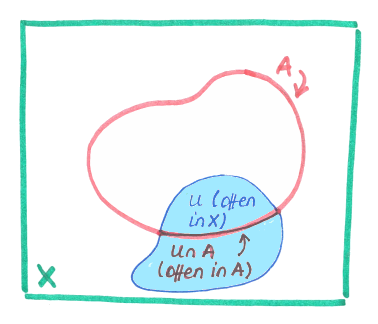
\includegraphics[height=4.5cm]{abb/teilraumtop.png}
        \caption{Teilraumtopologie}
        \label{fig:teilraumtop}
    \end{figure}
%    
%        
    \begin{bsp}[Teilraumtopologie Standardbeispiel]\ \\
        In der Teilraumtopologie von ${\rand A = \{\frac{1}{2^n} \mid n \in \N\} \cup \{0\}}$ (siehe Bsp.~\ref{bsp:standardbsp}) sind alle Mengen $M$ 
        \begin{itemize}
            \item abgeschlossen, die die $0$ enthalten oder für die  $M$ \textit{keine} Häufungspunkte hat.
            \item offen, die die $0$ \textit{nicht} enthalten oder für die $\rand A \setminus M$ \textit{keine} Häufungspunkte hat.
        \end{itemize}
        Dies ist eine einfache Folgerung aus der Eigenschaft von $A$, $0$ als einzigen Häufungspunkt zu haben. 
        Damit sind sowohl ${\HP(M)}$ als auch ${\HP(\rand A \setminus M)}$ ${\{0\}}$ oder $\varnothing$.
        Zusammen mit \\
        ${\cl(M) = M \cup \HP(M)}$ und ${\op(M) = M \setminus \HP(\rand A \setminus M)}$ ergeben sich die Aussagen.
    \end{bsp}
%
%
    Analog zu den offenen Mengen entstehen die abgeschlossenen Mengen in $A \subseteq X$ durch Schnitte mit in $X$ abgeschlossenen Mengen.
    %
    \begin{satz} \label{satz:trAbg}\ \vspace{8pt}

        \noindent
        Sei $X$ ein topologischer Raum und $B \subseteq A \subseteq X$. Dann gilt
        \begin{align*}
            B \in \abg_A \quad \quad \Leftrightarrow \quad \quad \exists\: B' \in \abg_X : B = B' \cap A 
        \end{align*}
        (Beweis siehe Anhang \ref{anh:trAbg})
        
    \end{satz}
    %(Beweis siehe \ref{anh:trAbg})
%
%
    Ist $A \subseteq X$ offen in $X$, so sind alle in $A$ offenen Mengen auch offen in $X$. Analoges gilt für abgeschlossene Mengen.
    %
    \begin{kor}\label{kor:OX-OA-CX-CA}
        Seien $X$ ein topologischer Raum und $B \subseteq A \subseteq X$. Dann gelten:
        \begin{enumerate}
            \item $A \in \offen_X \to (\: B \in \offen_A \leftrightarrow B \in \offen_X \:)$
            \item $A \in \abg_X \to (\: B \in \abg_A \leftrightarrow B \in \abg_X \:)$
        \end{enumerate}
    \end{kor}
    %
    \begin{bew}\ 
        \begin{enumerate}
            \item Sei $A \in \offen_X$. Falls $B \in \offen_A$ ist, so gibt es ein $U \in \offen_X$ mit $B = U \cap A \in \offen_X$.\\
            Ist andererseits $B \in \offen_X$, so ist $B = A \cap B \in \offen_A$.
            \item Mit vorherigem Satz analog.
        \end{enumerate}
    \end{bew}
%
%
    Der folgende Satz wird in den Beweisen von \ref{satz:da1=da2} und \ref{kor:da1=da2} verwendet.
    %
    \begin{satz} \label{satz:dAB<clB}\ \vspace{8pt}

        \noindent
        Seien $X$ ein topologischer Raum und $B \subseteq A \subseteq X$. Dann gilt 
    %
        \begin{align*}
            \rand_A(B) \subseteq \cl_X(B).
        \end{align*}
    %	
        (Beweis siehe Anhang \ref{anh:dAB<clB})
    \end{satz}
%     (Beweis siehe \ref{anh:dAB<clB})
%
%
    Der folgende Satz wird zum Beweis von Korollar \ref{kor:cl-rand-A1-A2} verwendet.
    %
    \begin{satz}\label{satz:clA1-teil-clA2}\ \\
        Seien $X$ ein topologischer Raum, ${A_1, A_2 \subseteq X}$ und ${B \subseteq A_1 \cap A_2}$ mit ${\cl_{A_1}(B) \subseteq A_2}$. Dann gilt ${\cl_{A_1}(B) \subseteq \cl_{A_2}(B)}$.\\
        (Beweis siehe Anhang \ref{anh:clA1-teil-clA2})
    \end{satz}
    %
%     (Beweis siehe \ref{anh:clA1-teil-clA2})
%
%
    Für einen topologischen Raum $X$ und Teilmengen $A_1, A_2, B \subseteq X$ mit $B \subseteq A_1 \cap A_2$ muss nicht notwendigerweise gelten $\cl_{A_1}(B) \subseteq A_2$.
    %
    \begin{gegenbsp}
        Man nehme $X = \{0,1\}, \offen_X = \{\varnothing, \{0,1\}\}, A_1 = X, A_2 = \{0\}, B = \{0\}$. Dann ist $\abg_X = \{\varnothing, \{0,1\}\}$ also $\abg_{A_1} = \{\varnothing, \{0,1\}\}$ und damit $\cl_{A_1} = \{0,1\} \nsubseteq A_2$
    \end{gegenbsp}
%
% 		\todo[inline]{FL: müsste es nach ``damit'' heißen:
% 		$\cl_{A_1}(B) = \{0,1\} \nsubseteq A_2$ ?\\
% 		-> BH: das ist richtig}
%
    Folgender Satz besagt jedoch, dass diese Aussage gilt, falls $A_1$ und $A_2$ Ränder von Mengen sind.
    %
    \begin{satz}\label{satz:cl-dA1-dA2}\ \\
        Seien $X$ ein topologischer Raum, $A_1, A_2 \subseteq X$ und \\
        $B \subseteq \rand A_1 \cap \rand A_2$.
        Dann ist $\cl_{\rand A_1}(B) \subseteq \rand A_2$.\\
        (Beweis siehe Anhang \ref{anh:cl-dA1-dA2})
    \end{satz}
    %
%     (Beweis siehe \ref{anh:cl-dA1-dA2})
%
%
    \begin{kor}\label{kor:cl-rand-A1-A2}
        Seien $X$ ein topologischer Raum, $A_1, A_2 \subseteq X$ und $B \subseteq \rand A_1 \cap \rand A_2$.\\
        Dann ist ${\cl_{\rand A_1}(B) = \cl_{\rand A_2}(B)}$.
    \end{kor}
%
    \begin{bew}
        Aus dem vorherigen Satz folgen $\cl_{\rand A_1}(B) \subseteq \rand_{A_2}B$ und $\cl_{\rand A_2}(B) \subseteq \rand_{A_1}B$. Deshalb lässt sich mit Satz \ref{satz:clA1-teil-clA2} folgern \\
        ${\cl_{\rand A_1}(B) \subseteq \cl_{\rand A_2}(B)}$ und ${\cl_{\rand A_2}(B) \subseteq \cl_{\rand A_1}(B)}$.
    \end{bew}
%
    Unter den Voraussetzungen von Korollar \ref{kor:cl-rand-A1-A2} gilt nicht notwendigerweise ${\op_{\rand A_1}(B) = \op_{\rand A_2}(B)}$.
%    
    \begin{gegenbsp}\label{gegenbsp-teiltop}\ \\
        Als Gegenbeispiel wähle $X = \R^2$, ${A_1 = \{(x,y) \in \R^2 \mid x*y < 0\}}$, ${A_2 = \{(x,y) \in \R^2 \mid x > 0, y > 0\}}$, \\
        ${B = \{0\} \times (0, \infty) \cup (0,\infty) \times \{0\}}$.\\
        Dann ist ${(0,0) \notin \op_{\rand A_1}(B)}$ aber ${(0,0) \in \op_{\rand A_2}(B)}$.
    \end{gegenbsp}
%
    \begin{figure}[ht]
        \centering
        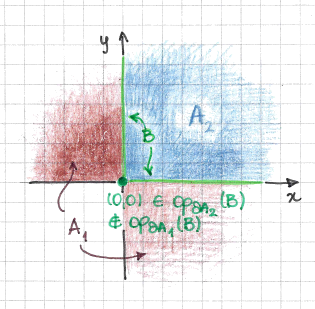
\includegraphics[height=7cm]{abb/gegenbsp-teilraumtop.png}
        \caption{Zu Gegenbeispiel \ref{gegenbsp-teiltop}}
        \label{fig:gegenbsp-teilraumtop}
    \end{figure}
%
    Daraus folgt, dass sich die Teilraumtopologien auf den Rändern von Mengen unter gewissen Bedingungen ähneln.
%
    \begin{satz}\label{satz:da1=da2} \ \vspace{8pt}

        \noindent
        Sei $X$ ein topologischer Raum. Seien $A_1, A_2 \subseteq X$ und $B \subseteq A_1 \cap A_2$ so, dass
    %
        \begin{align*}
            \exists\: \, U \in \offen_X: (\: \cl_X(B) \subseteq U \:\land\: U \cap A_1 = U \cap A_2 \:)
        \end{align*}
    %
        gilt. Dann gilt auch  
    %
        \begin{align*}
            \rand_{A_1}(B) = \rand_{A_2}(B).
        \end{align*}
        %
        (Beweis siehe Anhang \ref{anh:da1=da2})
        
    \end{satz}
%     (Beweis siehe \ref{anh:da1=da2})
%
%
    \begin{kor}\label{kor:da1=da2} \ \vspace{8pt}

        \noindent
        Sei $X$ ein topologischer Raum. Seien $A_1, A_2 \subseteq X$ und $B \subseteq A_1 \cap A_2$ so, dass
    %
        \begin{align*}
            \exists\: \, U \in \offen_X: (\: \cl_X(B) \subseteq U \:\land\: U \cap A_1 = U \cap A_2 \:)
        \end{align*}
    %
        gilt. Dann gelten auch  
    %
        \begin{enumerate}
            \item \label{kor:da1=da2.1} $\cl_{A_1}(B) = \cl_{A_2}(B)$
            \item \label{kor:da1=da2.2} $\op_{A_1}(B) = \op_{A_2}(B)$
            %\item \label{kor:da1=da2.3} $\co_{A_1}(B) = \co_{A_2}(B)$
            %\item \label{kor:da1=da2.4} $\oc_{A_1}(B) = \oc_{A_2}(B)$
        \end{enumerate} 
        (Beweis siehe Anhang \ref{anh:kor.da1=da2})
    \end{kor}
%     (Beweis siehe Anhang \ref{anh:kor.da1=da2})
    %\todo[inline]{3 und 4 auslagern, da co und oc noch nicht eingeführt sind}
    
    
    
    
    
    
                    %%%%%%%%%%%%%%%%%%%%%%%%%%%%%%%%%%%%%%
                    %%%                                %%%
%%%%%%%%%%%%%%%%%%%%%%%   Topologie metrischer Räume   %%%%%%%%%%%%%%%%%%%%%%%%%%%%%
                    %%%                                %%%
                    %%%%%%%%%%%%%%%%%%%%%%%%%%%%%%%%%%%%%%


\section{Topologie metrischer Räume}\label{sec:top-metr-raeume}

    Der hier vorgestellte Interpretationsansatz arbeitet mit Teilmengen des $\R^3$ und nutzt die topologische Struktur, die dieser Raum durch seine Metrik mit sich bringt.
    In diesem Abschnitt geht es darum, wie Metriken -- insbesondere die euklidische Metrik auf $\R^n$ -- Topologien erzeugen.
    
    Ein
    \marginpar{metrischer Raum}
    metrischer Raum ist eine Menge mit einer Metrik, also einer Abbildung, die anschaulich gesprochen je zwei Punkten ihren Abstand zuordnet.
    %
    \begin{dfn}[Metrischer Raum]\label{def:metr}\ \vspace{8pt}

        \noindent
        Ein \thmemph{metrischer Raum} ist ein Paar $(X,d)$ bestehend aus
    %
        \begin{itemize}
            \item einer Menge $X$ (\thmemph{Grundmenge}) und
            \item einer Abbildung $ d: X^2 \rightarrow \R_0^+$ (\thmemph{Metrik})
        \end{itemize}
    %
        so dass für alle $x$, $y$ und $z$ aus $X$ gelten
    %
        \begin{enumerate}
            \item $d(x,y) = 0 \quad \quad \Leftrightarrow \quad \quad x=y \qquad$ (positive Definitheit) 
            \item $d(x,y) = d(y,x) \qquad$ (Symmetrie)
            \item $d(x,y) + d(y,z) \geq d(x,z) \qquad$ (Dreiecksungleichung)
        \end{enumerate}
    %	
    \end{dfn}
%
%
    Die
    \marginpar{$\varepsilon$-Umgebung}
    $\varepsilon$-Umgebung eines Punktes besteht aus allen Punkten, die ihm $\varepsilon$-nahe sind, also einen kleineren Abstand als $\varepsilon$ haben.
% 		\todo[inline]{Zwei Quellen, in denen ich geschaut habe, nehmen dem Satz hierüber
% 		entsprechend $d(x,y) < \varepsilon$ in der Definition, statt $\leq$ darin. ``(offene)'' Umgebung würde auch dazu passen. Ich bin mir dennoch nicht 100\% sicher, was Du haben willst, daher als Kommentar.\\
% 		-> BH: <}
    %
    \begin{dfn}[$\varepsilon$-Umgebung]\label{def:eps-umg}\ \vspace{8pt}

        \noindent
        Seien (X,d) ein metrischer Raum, $x \in X$, $\varepsilon > 0$. Dann ist
        \begin{align*}
            \ball_\varepsilon(x) := \{y \in X \mid d(x,y) < \varepsilon \}
        \end{align*}
        die (offene) \thmemph{$\varepsilon$-Umgebung} von $x$.
        
    \end{dfn}
%
%
    In
    \marginpar{Topologie metrischer Räume}
    einem metrischen Raum ist ein innerer Punkt einer Menge ein Punkt, der eine $\varepsilon$-Umgebung hat, die ganz in dieser Menge liegt. Dies führt zu folgender Definition für offene Mengen in metrischen Räumen.
%
    \begin{dfn}[Topologie metrischer Räume] \label{def:topMet} \ \vspace{8pt}

        \noindent
        Sei $(X,d)$ ein metrischer Raum. Dann ist
        \begin{align*}
            \offen_d := \{A \subseteq X \mid \forall\: a \in A \; \exists\: \varepsilon > 0: \ball_\varepsilon(a) \subseteq A \}
        \end{align*}
        die von \thmemph{$d$ induzierte Topologie} auf $X$.
        
    \end{dfn}
%
    Der folgende Satz besagt, dass das so definierte Mengensystem tatsächlich im Sinne von \ref{def:top} eine Topologie ist.
    %
    \begin{satz}
        Sei $(X,d)$ ein metrischer Raum. Dann ist $(X,\offen_d)$ ein topologischer Raum.
    \end{satz}
    %
    Der Beweis ist einfach und ist unter anderem in [\cite{manetti-m-2015--a}] zu finden (Definition 3.4).

    Die topologischen Symbole einer durch eine Metrik $d$ induzierten Topologie kennzeichnen wir durch ein tiefgestelltes $d$.
    %
    \begin{nota} \ \vspace{8pt}

        \noindent
        Sei $(X,d)$ ein metrischer Raum. Wir bezeichnen 
        \begin{itemize}
        \item die \thmemph{Menge der abgeschlossenen Mengen} in $X$ mit $\abg_d$
        \item den \thmemph{Kernoperator} in $X$ mit $\op_d$
        \item den \thmemph{Abschlussoperator} in $X$ mit $\cl_d$
        \item den \thmemph{Randoperator} in $X$ mit $\rand_d$
        %\item den $oc$-Operator in $X$ mit $oc_d$
        %\item den $co$-Operator in $X$ mit $co_d$
        \end{itemize}
    \end{nota}
%
%
    Die abgeschlossenen Mengen in einem metrischen Raum lassen sich auf ähnliche Weise definieren wie die offenen.
    %
    \begin{satz} \label{satz:Cd} \ \hspace{8pt}

        \noindent
        Sei $(X,d)$ ein metrischer Raum. Dann gilt
        \begin{align*}
            \abg_d := \{A \subseteq X \mid \forall\: x \in X (\: \forall\: \varepsilon > 0 : \ball_\varepsilon \cap A \neq \varnothing \rightarrow x \in A \:) \}
        \end{align*}
        
    \end{satz}
    %
    \begin{bew}
        \begin{align*}
            &\abg_d = \{A \subseteq X \mid X \setminus A \in \offen_d\} \\
            &= \{A \subseteq X \mid \forall\: x \in X \setminus A \; \exists\: \varepsilon > 0 : \ball_\varepsilon(x) \subseteq X \setminus A\} \\
            &= \{A \subseteq X \mid \forall\: x \in X (\: x \notin A \rightarrow \exists\: \varepsilon > 0 : \ball_\varepsilon(x) \cap A = \varnothing \:) \} \\
            &= \{A \subseteq X \mid \forall\: x \in X (\: \forall\: \varepsilon > 0 : \ball_\varepsilon(x) \cap A \neq \varnothing \rightarrow x \in A \:) \} 
        \end{align*}
    \end{bew}
%
%
%     \begin{satz} \label{satz:dAabg}
%         Seien $(X,d)$ ein metrischer Raum, $A \subseteq X$. Dann gilt $\rand_d A \in \abg_d$.
%     \end{satz}
%     (Beweis siehe \ref{anh:dAabg})
%      % bem: unnötig, da schon in Korollar \ref{kor:rand-abg} allgemein bewiesen
%
%
%     \begin{kor} \label{kor:BinCA-BinC}
%         Seien $(X,d)$ ein metrischer Raum, $A \subseteq X$, $B \in \abg_{\rand_d A}$. Dann gilt: $B \in \abg_d$.
%     \end{kor}
%     %
%     \begin{bew}
%         Aus Korollar \ref{kor:rand-abg} folgt $\rand_d A \in \abg$. Aus Satz \ref{satz:trAbg} wissen wir da $B \in \abg_{\rand_d A}$ ist gibt es ein $B' \in \abg_d$ mit $B = B' \cap \rand_d A$. Als Schnitt abgeschlossener Mengen ist dann $B$ auch abgeschlossen (vgl. Satz \ref{satz:cl}).
%     \end{bew}
    % bem: unnötig, da Spezialfall von Korollar \ref{kor:OX-OA-CX-CA}
%
%
%     \todo[inline]{prüfen, ob folgender Satz raus kann, da er nicht verwendet wird}
%     \begin{satz}\label{satz:ball}
%     Sei $(X,d)$ ein metrischer Raum, $x \in X$. Seien $\varepsilon, \delta \in \R$ mit $0 < \varepsilon< \delta$. Dann gilt: $\cl_d(\ball_\varepsilon(x)) \subseteq \ball_\delta(x)$.
%     \end{satz}
%     %
%     \begin{bew}
%     Sei $y \in \cl_d(\ball_\varepsilon(x))$. Dann gilt für alle $\eta > 0$:\\ $\ball_\eta(y) \cap U_\varepsilon(x) \neq \varnothing$. Sei $\eta = \delta - \varepsilon$. Sei $z \in U_\eta(y) \cap U_\varepsilon(x)$. Nach der Dreiecksungleichung gilt dann:
%     $$d(x,y) \leq d(x,z) + d(z,y) < \varepsilon + \eta = \delta.$$
%     Also ist $y \in \ball_\delta(x)$.
%     \end{bew}
%
%
    Auf
    \marginpar{Standardmetrik des $\R^n$}
    $\R^n$ liefert der euklidische Abstand, der mit Hilfe des Skalarprodukts berechnet werden kann, eine Metrik -- die sogennannte Standardmetrik des $\R^n$.
    %
    \begin{dfn}[Standardmetrik des $\R^n$]\label{def:standardmetrik}\ \vspace{8pt}

        \noindent
        Auf $\R^n$ ist die \thmemph{Standardmetrik} $d_n : \R^n \times \R^n \rightarrow \R_0^+$ definiert durch
        \begin{align*}
            d_n(x,y) = \sqrt{(x-y)^2}
        \end{align*}
        
        \noindent
        Die durch die Standardmetrik induzierte Topologie auf $\R^n$ bezeichnen wir mit $\offen_n$.
        
    \end{dfn}
%
    \begin{konv}\label{konv:d3}
        Statt $d_3$ schreiben wir auch einfach $d$.	
    \end{konv}
%    
    \begin{bem}
        Die durch die Standardmetrik induzierte Topologie auf $\R$ stimmt mit der in Bsp.~\ref{bsp:standard-r} definierten Standardtopologie überein.
    \end{bem}
%
%
    Der folgende Satz besagt, dass ein stetiger Weg, der in einer Menge beginnt und außerhalb von ihr endet, immer einen Randpunkt passieren muss. Er wird zum Beweis von Satz \ref{satz:r2} verwendet und lässt sich möglicherweise nutzen, um zu zeigen, dass gewisse Punkte äußere Randpunkte sind (zum Begriff des äußeren Randes siehe Abschnitt \ref{sec:aeusserer-rand}).
    %
    \begin{satz}\label{satz:weg} %verwendung: {satz:r2}
        Sei $X$ ein topologischer Raum. Sei $A \subset X$. Seien $x \in A$, $y \in X \setminus A$. Seien $a,b \in \mathbb{R}$ mit $a < b$. Sei $\gamma : [a,b] \to X$ ein stetiger Weg mit $\gamma(a) = x$ und $\gamma(b) = y$. Dann gibt es ein $t \in [a,b]$ mit $\gamma(t) \in \rand A$.
    \end{satz}
%    
    \begin{figure}[ht]
        \centering
        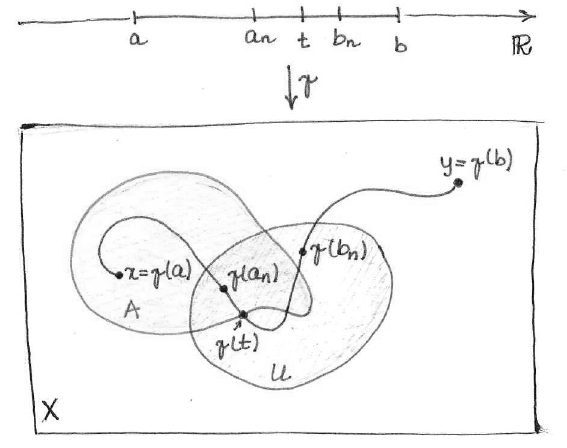
\includegraphics[height=5cm]{abb/weg_sw.png}
        \caption{Zum Beweis von Satz \ref{satz:weg}}
        \label{fig:weg}
    \end{figure}
%
    \begin{bew}
        Definiere eine Intervallschachtelung $([a_i, b_i])_{i \in \N}$ auf folgende Weise:
        \begin{enumerate}
            \item $a_0 = a, b_0 = b$
            \item Wenn $\gamma(\frac{a_i + b_i}{2}) \in A$, so setze $a_{i+1} = \frac{a_i + b_i}{2}$, $b_{i+1} = b_i$\\
            Ansonsten setze $a_{i+1} = a_i$, $b_{i+1} = \frac{a_i + b_i}{2}$
        \end{enumerate}
        Sei $t$ die eindeutige reelle Zahl, die in allen Intervallen $[a_i, b_i]$ enthalten ist.\\
        Behauptung: Dann ist $\gamma(t) \in \rand A$.\\
        Beweis der Behauptung: Zu zeigen ist: 
        \[\forall\: U \in \offen_X: (\: \gamma(t) \in U \rightarrow (\: U \cap A \neq \varnothing \:\land\: U \setminus A \neq \varnothing \:) \:).\]
        Nach Konstruktion der Intervallschachtelung gelten:
        \begin{enumerate}
        \item $\forall\: \varepsilon > 0\ \exists\: n \in \N\ \forall\: i \geq n: \ball¸_\varepsilon(t) \subseteq [a_i,b_i]$
        \item $\forall\: i \in \N : (\: \gamma(a_i) \in A \:\land\: \gamma(b_i) \notin A \:)$
        \end{enumerate}
        Sei nun ${U \in \offen_X}$. Da $\gamma$ stetig ist, ist ${\gamma^{-1}(U) \in \offen_{\R}}$. Da ${t \in \gamma^{-1}(U)}$ ist, gibt es also ein ${\varepsilon > 0}$ mit ${\ball_\varepsilon(t) \subseteq \gamma^{-1}(U)}$.\\
        Sei ${n \in \N}$ mit ${[a_i, b_i] \subseteq \ball_\varepsilon(t)}$ für alle ${i \geq n}$, dann sind \\
        ${\gamma(a_n) \in U \cap A}$ und ${\gamma(b_n) \in U \setminus A}$.
    \end{bew}

% 
% \chapter{Weitere topologische Begriffe}\label{chap:topologie-erweiterung}

In diesem Kapitel definiere ich 
% in den Abschnitten \ref{sec:lokale-gleichheit}--\ref{sec:aeusserer-rand} 
eigene Begriffe auf topologischen Räumen,
die ich für die formale Definition der \strukt benötige.
Dazu gehören:
\begin{enumerate}
    \item die \textemph{lokale Gleichheit} als Grundlage für die Definition der Objektäquivalenz
    \item \textemph{einfache Mengen} als Kandidaten für Raumregionen sowie euklidische Flächen und Linien
    \item der \textemph{äußere Rand}: euklidische Flächen, Linien und Punkte sind ausgewählte Teilmengen des äußeren Randes.
\end{enumerate}
%Außerdem werden in Abschnitt \ref{ssec:notationelle-konv} vereinfachte Notationen für oft gebrauchte Operatoren eingeführt.


    
                            %%%%%%%%%%%%%%%%%%%%%%%%%%
                          %%%                        %%%
%%%%%%%%%%%%%%%%%%%%%%%%%%%      Lokale Gleichheit      %%%%%%%%%%%%%%%%%%%%%%%%%%%%%%%%%%
                          %%%                        %%%
                            %%%%%%%%%%%%%%%%%%%%%%%%%%


\section{Lokale Gleichheit}\label{sec:lokale-gleichheit}
    Zwei
    \marginpar{lokale Gleichheit}
    Flächenrepräsentanten sollen objektäquivalent sein, 
    wenn sie koinzidieren und die Raumregionen, die sie begrenzen \glqq von der gleichen Seite kommen\grqq. 
    Analoges gilt für Linien- und Punktrepräsentanten. 
    Der Begriff der lokalen Gleichheit ist ein Ansatz, formal zu beschreiben, was es heißt, \glqq von der gleichen Seite\grqq\ zu kommen.
    
    Anschaulich gesprochen sind zwei Teilmengen eines topologischen Raumes dann lokal gleich bezüglich eines Punktes, wenn dieser eine Umgebung hat, in der sie nicht zu unterscheiden sind.
    Sie sind lokal gleich bezüglich einer Menge, wenn sie lokal gleich sind bezüglich jeden Punktes dieser Menge.
    
%     Eine anschauliche Vorstellung dieses Begriffs lässt sich durch das Ameise-im-Nebel-Bild beschreiben:\\
%     Eine Ameise kann sich innerhalb einer Fläche $B$ frei bewegen. Sie kann in alle Richtungen sehen, aber nur ein kleines Stück, denn es herrscht dichter Nebel. Dieser Nebel ist möglicherweise unterschiedlich dicht an verschiedenen Stellen. Zwei Raumregionen $A_1$ und $A_2$ sind lokal gleich bzgl. $B$, wenn es einen \glqq Nebel\grqq\ gibt, so dass die Ameise $A_1$ und $A_2$ nicht unterscheiden kann.

    \begin{dfn}[Lokal gleich]\label{def:lok-gleich}\ \\
        Seien $X$ ein topologischer Raum, $A_1, A_2 \subseteq X$.
        $A_1$ und $A_2$ sind \thmemph{lokal gleich} 
        \begin{itemize}
            \item in einem Punkt ${p \in X}$, falls es ein ${U \in \offen(p)}$ gibt mit \\
            ${U \cap A_1 = U \cap A_2}$.
            \item bzgl. einer Menge $M \subseteq X$, falls $A_1$ und $A_2$ in jedem Punkt von $M$ lokal gleich sind.
        \end{itemize}
        Wir schreiben ${A_1 =_x A_2}$, falls $A_1$ und $A_2$ lokal gleich sind in bzw. bzgl. $x$.
    \end{dfn}
    
    \begin{bem}\ \\
     In einem metrischen Raum lässt sich lokale Gleichheit in einem Punkt $p$ äquivalent definieren durch:
     $$ A_1 =_p A_2 \quad \quad \Leftrightarrow \quad \quad \exists\: \varepsilon > 0 : B_\varepsilon(p) \cap A_1 = B_\varepsilon(p) \cap A_2.$$
    \end{bem}
    
    \begin{bsp}\label{bsp:lok-gleich}\ \\
     $A_1 := (0,1)^2$ und $A_2 := (0,2) \times (0,1)$ sind lokal gleich bzgl. $M_1 := (0,1) \times \{0\}$ nicht jedoch bzgl. $M_2 := [1,2] \times \{1\}$, denn für jeden Punkt $p_1 = (x_1,0)$ ist mit $\varepsilon_1 := min\{x_1,1-x_1\}$ $B_{\varepsilon_1/2}(p_1)$ eine Umgebung von $p_1$ auf der sich $A_1$ und $A_2$ nicht unterscheiden.
     Aber für $(1,1) \in M_2$ gibt es keine Umgebung $U$ mit $U \cap A_1 = U \cap A_2$ (siehe Abbildung \ref{fig:lok-gleich}).
    \end{bsp}
    
    \begin{figure}[ht]
        \centering
        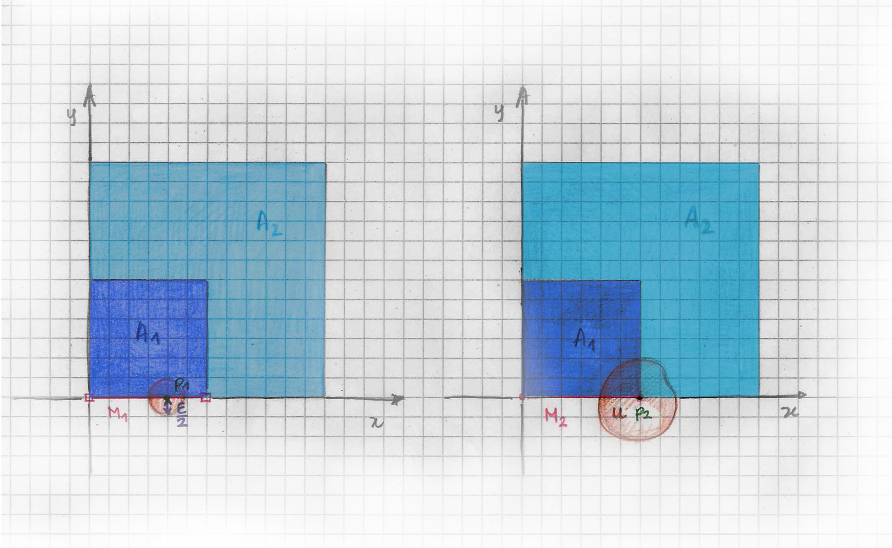
\includegraphics[width=\textwidth]{abb/lok-gleich.png}
        %\caption[Lokale Gleichheit]{Zu Beispiel \ref{bsp:lok-gleich}}
        \caption{Zu Beispiel \ref{bsp:lok-gleich}}
        \label{fig:lok-gleich}
    \end{figure}

        
%     Eine anschauliche Vorstellung der lokalen Gleichheit lässt sich durch das Ameise-im-Nebel-Bild gewinnen:\\
%     Eine Ameise kann sich auf ganz $B$ frei bewegen. Sie kann in alle Richtungen sehen, aber nur ein kleines Stück, denn es herrscht dichter Nebel. Dieser Nebel ist möglicherweise unterschiedlich dicht an verschiedenen Stellen. $A_1$ und $A_2$ sind lokal gleich bzgl. $B$, wenn es einen \glqq Nebel\grqq\ gibt, so dass die Ameise $A_1$ und $A_2$ nicht unterscheiden kann.
%     
    
    \begin{satz}\label{satz:lokale-gleichheit-aer}
        Die lokale Gleichheit in einem Punkt ist eine Äquivalenzrelation.\\
        (Beweis: siehe Anhang \ref{anh:lokale-gleichheit-aer})
    \end{satz}
%     Beweis: siehe Anhang \ref{anh:lokale-gleichheit-aer}
    
    \begin{kor}\label{kor:lokale-gleichheit-aer}
     Die lokale Gleichheit bzgl. einer festen Menge ist eine Äquivalenzrelation.\\
     (Beweis: direkte Folgerung aus dem vorhergehenden Satz.)
    \end{kor}
    
    Die folgenden Sätze besagen, dass lokal gleiche Mengen auch lokal die gleichen Randpunkte haben.
    \begin{satz}\label{satz:rand-lokal-gleich}\ \\
        Seien $X$ ein topologischer Raum, $p \in X$, $A,B \subseteq X$ mit $A =_p B$. Falls $p \in \rand A$ ist, so ist $p$ auch in $\rand B$.\\
        (Beweis: siehe Anhang \ref{anh:rand-lokal-gleich})
    \end{satz}
%     Beweis: siehe \ref{anh:rand-lokal-gleich}
    
    \begin{kor}\ \\ 
        Seien $X$ ein topologischer Raum, $A_1, A_2 \subseteq X$, $B \subseteq \rand A_1$, $A_1 =_{B} A_2$. Dann ist $B \subseteq \rand A_2$.\\
        (Beweis: direkte Folgerung aus dem vorhergehenden Satz.)
    \end{kor}
%     Beweis: direkte Folgerung aus dem vorhergehenden Satz.
    \todo[inline]{FL: Ich hoffe, die Korrektur zweier Auftreten von $B_1$ zu $B$ ist korrekt.\\
    -> BH: bestimmt!}


    
    
                            %%%%%%%%%%%%%%%%%%%%%%%%%
                          %%%                       %%%
%%%%%%%%%%%%%%%%%%%%%%%%%%%      Einfache Mengen      %%%%%%%%%%%%%%%%%%%%%%%%%%%%%%%%%%
                          %%%                       %%%
                            %%%%%%%%%%%%%%%%%%%%%%%%%

\section{Einfache Mengen}\label{sec:einf-mengen}
% \cFLimp[inline]{TODO:
% §, der beschreibt, wozu der nächste oder die nächsten Begriffe notwendig sind.
% 
% Zum Aufbau:\\
% Wozu werden `einfache Mengen' dienen? Wie lassen sie sich in 1-3 Sätzen intuitiv beschreiben?
% Ggf.\ wozu wird `maximaldimensional' dabei benötigt? Wichtiger: Intuitive Beschreibung.
% } %\cFLimp
% 
% \todo[inline]{Die Verwendeng der Begriffe Flächen-, Linien-, Punktrepräsentant vs Grenzfläche, -linie, -punkt in Übereinstimmung mit Kapitel \ref{sec:grundideen} überprüfen}

Einfache Mengen werden die Kandidaten für Raumregionen, euklidische Flächen und Linien sein.
In Abschnitt \ref{sec:zusammenfassung} wurden einige wünschenswerte Eigenschaften dieser Objekte zusammengefasst.
Wie wir im Folgenden sehen werden, schließen einfache Mengen einige offensichtlich unerwünschte Fälle aus. 
Ob sie ausreichend sind, um alle gewünschten Eigenschaften zu gewährleisten, bleibt noch zu untersuchen (vgl.\ Abschnitt \ref{sec:offene-fragen}).


\subsection{Definitionen und Eigenschaften}
\todo[inline]{FL: Alternative Überschrift: Charakterisierung\\
Überschrift eingefügt, um die einzelne Überschrift '5.2.1 Ein Beispiel' zu vermeiden, da in aller Regel mind.\ zwei Unterüberschriften genutzt werden, wenn überhaupt untergliedert wird.\\
- BH: ``Definitionen und Eigenschaften'' finde ich OK}
In
\marginpar{maximaldimensional}
unserer Vorstellung sind Raumregionen überall dreidimensional (R1). D.h. insbesondere, sie haben keine \glqq niederdimensionalen Ausläufer\grqq.
Eingebettet in einen dreidimensionalen Raum sind Raumregionen also maximaldimensionale Teilmengen.

    \begin{dfn}[Maximaldimensional]\label{def:maxdim}\ \\
        Sei $X$ ein topologischer Raum. Eine Teilmenge $A \subseteq X$ heißt \thmemph{maximaldimensional}, wenn für jeden Punkt $a \in A$ gilt:
        $$\forall\: U \in \offen_X(a) : U \cap \op_X(A) \neq \varnothing$$ 
    \end{dfn}
    
    
    Die folgenden Sätze geben zwei einfach zu zeigende Eigenschaften für maximaldimensionale Mengen an, die in einigen Beweisen genutzt werden.
    %
    \begin{satz}\label{satz:offen-maxdim}
        Jede offene Menge ist maximaldimensional.\\
        (Beweis: trivial)
    \end{satz}
%     Beweis: trivial
    
    
    \begin{satz}\label{satz:abschluss-maxdim}
        Der Abschluss jeder maximaldimensionalen Menge ist maximaldimensional.
    \end{satz}
    
    \begin{bew}
        Sei $A$ maximaldimensional. 
        Angenommen $\cl(A)$ ist nicht maximaldimensional.
        Dann gibt es ein $x \in \cl(A)$ und eine offene Umgebung $U \in \offen(x)$, s.d. $U \cap \op(cl(A)) = \varnothing$ ist.
        Dann ist natürlich auch $U \cap \op(A) = \varnothing$.
        Da $A$ maximaldimensional ist, muss dann auch $U \cap A = \varnothing$ sein, denn falls es eine $y$ in $U \cap A$ gäbe, wäre $U$ auch eine offene Umgebung von $y \in A$ und somit müsste $U \cap \op(A) \neq \varnothing$ sein.
        Damit kann $x$ nicht in $\cl(A)$ sein. 
        $\lightning$
    \end{bew}


    Die folgenden drei Beispiele zeigen maximaldimensionale und nicht maximaldimensionale Mengen im $\R^2$.
    %
    \begin{bsp}\label{bsp:maximaldimensional-1}
        $A := \{(x,y) \in \R^2 \mid x^2 \leq y\} \subseteq \R^2$ ist maximaldimensional.
    \end{bsp}
    %
    \begin{bew}
        Sei $(a,b) \in A$. Sei $U \in \offen((a,b))$. Sei $\varepsilon > 0$ mit $B_\varepsilon((a,b)) \subseteq U$. Dann ist $(a,b+\varepsilon) \in U \cap \op(A)$.
    \end{bew}

    
    \todo[inline]{Bilder zu den Beispielen zusammenfassen}
    \begin{figure}[ht]
        \centering
        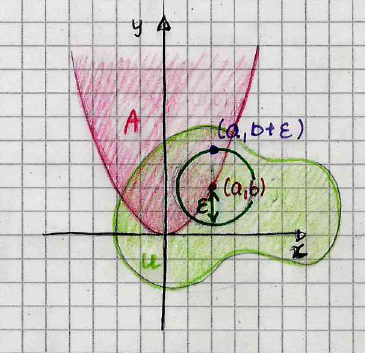
\includegraphics[width=5cm]{abb/maxdim-1.png}
%         \caption[Maximaldimensionale Menge]{Zu Beispiel \ref{bsp:maximaldimensional-1}}
        \caption{Zu Beispiel \ref{bsp:maximaldimensional-1}}
        \label{fig:maxdim-1}
    \end{figure}

    \begin{bsp}\label{bsp:maximaldimensional-2}
        $B := \{(x,y) \in \R^2 \mid x^2 \leq y\} \setminus \{0\} \times \R \subseteq \R^2$ ist maximaldimensional.
    \end{bsp}
    %
    \begin{bew}
        Sei $(a,b) \in B$. Sei $U \in \offen((a,b))$. Sei $\varepsilon > 0$ mit $B_\varepsilon((a,b)) \subseteq U$. Dann ist $(a,b+\frac{\varepsilon}{2}) \in U \cap \op(B)$.
    \end{bew}

    
    \begin{figure}[ht]
        \centering
        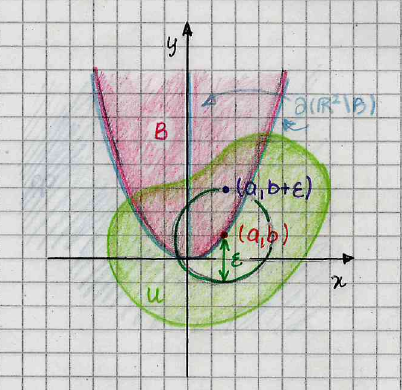
\includegraphics[width=5cm]{abb/maxdim-2.png}
        %\caption[Maximaldimensionale Menge]{Zu Beispiel \ref{bsp:maximaldimensional-2}}
        \caption{Zu Beispiel \ref{bsp:maximaldimensional-2}}
        \label{fig:maxdim-2}
    \end{figure}

    \begin{gegenbsp}\label{gegenbsp:maximaldimensional}
        $C := \{(x,y) \in \R^2 \mid x^2 \leq \max\{0,y\}\} \subseteq \R^2$ ist nicht maximaldimensional.
    \end{gegenbsp}
    %
    \begin{bew}
        Mit $A$ aus Bsp. \ref{bsp:maximaldimensional-1} sind $C = A \cup \{0\} \times \R$ und $\op(C) = \op(A) = \{(x,y) \in \R^2 \mid x^2 < y\}$. Also ist $(0,-2) \in C$, aber für $U := B_1((0,-2))$ ist $U \cap \op(C) = \varnothing$.
    \end{bew}

    
    \begin{figure}[ht]
        \centering
        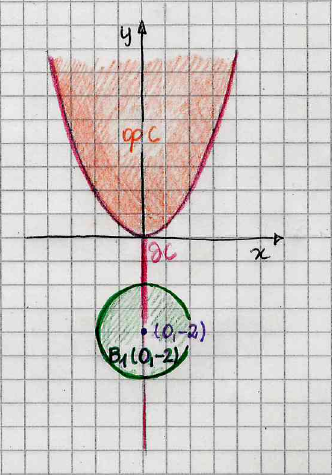
\includegraphics[width=5cm]{abb/nicht-maxdim.png}
        %\caption[Nicht-maximaldimensionale Menge]{Zu Beispiel \ref{gegenbsp:maximaldimensional}}
        \caption{Zu Beispiel \ref{gegenbsp:maximaldimensional}}
        \label{fig:nicht-maxdim}
    \end{figure}

    Obige
    \marginpar{Probleme mit maximaldimensionalen Mengen}
    Beispiele legen nahe, dass maximaldimensionale Mengen in $\R^n$ keine niederdimensionalen Ausläufer haben können.
    Sie können jedoch immer noch niederdimensionale Löcher aufweisen.
    Einfache Mengen im $\R^3$ können beispielsweise Kurven als Löcher haben und somit Randstücke, die nicht 2-dimensional sind, wie in (R2) gefordert. 
    Beispiel \ref{bsp:maximaldimensional-2} beschreibt eine 2-dimensionale Menge mit einem 1-dimensionalen Loch.
    
    Beispiel \ref{bsp:maximaldimensional-2} zeigt ein weiteres Problem, das in den Forderungen (R0) - (R2) nicht thematisiert wird. Diese Menge hat einen \glqq inneren\grqq\ Rand. Die positive $y$-Achse ist Rand der Menge $B$, obwohl $B$ sowohl links als auch rechts dieser Achse liegt. Für eine Linienregion, die Teil dieser Geraden ist, würde das bedeuten, dass nicht klar ist \glqq von welcher Seite\grqq die Flächenregion kommt, die sie begrenzt.
    
    Um
    \marginpar{einfache Menge}
    solche Fälle auszuschließen, soll auch das Komplement einer einfachen Menge maximaldimensional sein.

    \begin{dfn}[Einfache Menge, $\einf$, $\CO_X$, $\OC_X$]\label{def:einf}\ \\
        Sei $X$ ein topologischer Raum. Eine Teilmenge $A \subseteq X$ heißt 
        \begin{enumerate}
            \item \thmemph{einfach}, wenn sie und ihr Komplement $X \setminus A$ maximaldimensional sind,
            \item \thmemph{einfach abgeschlossen}, wenn sie einfach ist und abgeschlossen,
            \item \thmemph{einfach offen}, wenn sie einfach ist und offen.
        \end{enumerate}
        Die \thmemph{Menge der einfachen Mengen} in $X$ bezeichnen wir mit $\einf_X$, die der \thmemph{einfach abgeschlossenen Mengen} mit $\CO_X$ und die der \thmemph{einfach offenen Mengen} mit $\OC_X$.\\
        Wenn dies nicht zu Uneindeutigkeit führt, schreiben wir auch $\einf$, $\CO$ und $\OC$.
    \end{dfn}
    
    Wie sieht es nun mit der Einfachheit der obigen Beispiele aus?
    \begin{bsp}\label{bsp:einfach}
        $A = \{(x,y) \in \R^2 \mid x^2 \leq y\}$ aus Bsp. \ref{bsp:maximaldimensional-1} ist einfach.
    \end{bsp}
    %
    \begin{bew}
        Klar ist: $A$ ist maximaldimensional. Da $A$ abgeschlossen ist, ist ihr Komplement offen und somit auch maximaldimensional.
    \end{bew}

    \begin{gegenbsp}\label{gegenbsp:einfach-1}
        $B = \{(x,y) \in \R^2 \mid x^2 \leq y\} \setminus \{0\} \times \R$ aus Bsp. \ref{bsp:maximaldimensional-2} ist \textit{nicht} einfach.
    \end{gegenbsp}
    %
    \begin{bew}
        $B$ ist zwar maximaldimensional, aber $\R^2 \setminus B = \{(x,y) \in \R^2 \mid x^2 > y\} \cup \{0\} \times \R$ und somit ist $(0,2) \in \R^2 \setminus B$, aber $B_1((0,2)) \cap \op(\R^2 \setminus B) = B_1((0,2)) \cap \{(x,y) \in \R^2 \mid x^2 > y\} = \varnothing$.
    \end{bew}
    %
    \begin{figure}[ht]
        \centering
        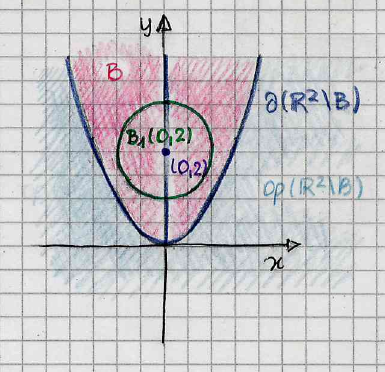
\includegraphics[width=5cm]{abb/nicht-einfach.png}
        %\caption[Nicht-einfache Menge]{Zu Beispiel \ref{gegenbsp:einfach-1}}
        \caption{Zu Beispiel \ref{gegenbsp:einfach-1}}
        \label{fig:nicht-einfach}
    \end{figure}

    \begin{gegenbsp}\label{gegenbsp:einfach-2}
        $C = \{(x,y) \in \R^2 \mid x^2 \leq \max\{0,y\}\}$ aus Gegenbsp. \ref{gegenbsp:maximaldimensional} ist nicht einfach, da nicht maximaldimensional.
    \end{gegenbsp}
    %
    Diese Beispiele legen nahe, dass einfache Mengen in $\R^n$ auch keine niederdimensionalen Löcher haben können.
    
    Die folgenden Sätze geben Eigenschaften von einfachen Mengen an, die für Beweise nützlich sein können.
    \begin{satz}\label{satz:einf-komplement}
        Sei $X$ ein topologischer Raum. Eine Teilmenge $A \subseteq X$ ist genau dann einfach, wenn ihr Komplement einfach ist.\\
        (Beweis trivial.)
    \end{satz}
%     Beweis trivial.
    
    
    \begin{satz}\label{satz:inneres-einf-offen}
        Das Innere jeder einfachen Menge ist einfach offen.
    \end{satz}
    
    \begin{bew}
        Sei $X$ eine topologischer Raum, $A \in \einf_X$. 
        Klar: $\op(A)$ ist offen und als offene Menge nach Satz \ref{satz:offen-maxdim} maximaldimensional.
        Zu zeigen ist also noch: $X \setminus \op(A)$ ist maximaldimensional.
        Da $A \in \einf_X$ ist, ist $X \setminus A$ maximaldimensional und damit nach Satz \ref{satz:abschluss-maxdim} auch $\cl(X \setminus A) = X \setminus \op(A)$.
    \end{bew}
    
    
    \begin{kor}
        Der Abschluss jeder einfachen Menge ist einfach abgeschlossen.
    \end{kor}
    
    \begin{bew}
        Wenn $A$ einfach ist, dann auch $X \setminus A$ und somit nach vorherigen Satz auch $\op(X \setminus A) = X \setminus \cl(A)$ und damit auch $\cl(A)$. 
        Abgeschlossen ist $\cl(A)$ sowieso.
    \end{bew}


    Die folgenden beiden Sätze stellen alternative Definitionen für einfache Mengen dar.
    \begin{satz}
        Sei $X$ ein topologischer Raum. Eine Teilmenge $A \subseteq X$ ist genau dann einfach, wenn für alle $x \in X$ und jede offene Umgebung $U$ von $x$ gilt:
        \begin{itemize}
            \item falls $x \in A$, so gilt $U \cap \op(A) \neq \varnothing$
            \item falls $x \notin A$, so gilt $U \setminus \cl(A) \neq \varnothing$
        \end{itemize}
        (Beweis trivial)
    \end{satz}
%     Beweis trivial


    Folgender Satz besagt, dass man zur Überprüfung der Einfachheit einer Menge nur Randpunkte untersuchen muss. 
    %Er bietet somit eine alternative Definition für einfache Mengen.
    %
    \begin{satz}\label{satz:alt-def-einf-1}
        Sei $X$ ein topologischer Raum, $A \subseteq X$. Dann ist $A$ einfach genau dann, wenn für alle $a \in \rand A$ gilt:
        $$\forall\: U \in \offen(a): (\: U \cap \op(A) \neq \varnothing \:\land\: U \setminus \cl(A) \neq \varnothing \:) $$
        (Beweis: siehe Anhang \ref{anh:alt-def-einf-1})
    \end{satz}
%     Beweis: siehe Anhang \ref{anh:alt-def-einf-1}
   
    Wie
    \marginpar{$\co$- und $\oc$-Operatoren}
    wir in \ref{kor:co(A)=A-oc(A)=A} sehen werden, lassen sich einfach abgeschlossene und offene Mengen auch als Fixpunkte zweier Operatoren verstehen, die ich mit $\co$ und $\oc$ bezeichne.
    %
    \begin{dfn}[$co$- und $oc$-Operator, Abgeschlossenes Inneres, innerer Abschluss]\label{def:cooc} \ \vspace{8pt}

        \noindent
        Für einen topologischen Raum $X$ definieren wir
        \begin{enumerate}
            \item den \thmemph{$\boldsymbol{co}$-Operator} $\co_X: 2^X \rightarrow 2^X$ durch
                \begin{align*}
                    \co_X := \cl_X \circ \op_X 		
                \end{align*} 
            \item den \thmemph{$\boldsymbol{oc}$-Operator} $\oc_X: 2^X \rightarrow 2^X$ durch
                \begin{align*}
                    \oc_X := \op_X \circ \cl_X 		
                \end{align*} 	
        \end{enumerate}	 

        \noindent
        $\co_X(A)$ nennen wir das \thmemph{abgeschlossene Innere}, $\oc_X(A)$ den \thmemph{inneren Abschluss} von $A$.
        
    \end{dfn}
    \todo[inline]{Beispiele}


    Die folgenden Sätze liefern hilfreiche Rechenregeln für den $\co$- und den $\oc$-Operator.
    %
    \begin{satz}[Eigenschaften des $\co$-Operators]\label{satz:co} \ \vspace{8pt}

        \noindent
        Sei $X$ ein topologischer Raum, $A, B \subseteq X$. Dann gelten
    %	
        \begin{enumerate}
            \item \label{satz:co.0} $\co(X \setminus A) = X \setminus \oc(A)$.
            \item \label{satz:co.1} $\co(A \setminus B) \subseteq \co(A) \setminus \oc(B)$.
            \item \label{satz:co.2} $A \in \abg \quad \Rightarrow \quad \co(A) \subseteq A$.
            \item \label{satz:co.3} $A \subseteq B \quad \Rightarrow \quad \co(A) \subseteq \co(B)$
            \item \label{satz:co.4} $\co(\co(A)) = \co(A)$.		
        \end{enumerate}	
        
        (Die Beweise für \ref{satz:co.0} - \ref{satz:co.3} folgen durch einfaches Anwenden der Rechenregeln für Kern- und Abschlussoperator (Sätze \ref{satz:cl} und \ref{satz:op}). Zu \ref{satz:co.4} siehe \ref{anh:co.4-oc.4}.)
    \end{satz}
    %
%     Die Beweise für \ref{satz:co.0} - \ref{satz:co.3} folgen durch einfaches Anwenden der Rechenregeln für Kern- und Abschlussoperator (Sätze \ref{satz:cl} und \ref{satz:op}). Zu \ref{satz:co.4} siehe \ref{anh:co.4-oc.4}.


    \begin{satz}[Eigenschaften des $\oc$-Operators] \label{satz:oc} \ \vspace{8pt}

        \noindent
        Sei $X$ ein topologischer Raum, $A, B \subseteq X$. Dann gelten
    %	
        \begin{enumerate}
            \item \label{satz:oc.0} $\oc(X \setminus A) = X \setminus \co(B)$.
            \item \label{satz:oc.1} $\oc(A \setminus B) \subseteq \oc(A) \setminus \co(B)$.
            \item \label{satz:oc.2} $A \in \offen \quad \Rightarrow \quad A \subseteq \oc(A)$.
            \item \label{satz:oc.3} $A \subseteq B \quad \Rightarrow \quad \oc(A) \subseteq \oc(B)$.
            \item \label{satz:oc.4} $\oc(\oc(A)) = \oc(A)$.
        \end{enumerate}	
        
        (Die Beweise für \ref{satz:oc.0} - \ref{satz:oc.3} folgen durch einfaches Anwenden der Rechenregeln für Kern- und Abschlussoperator (Sätze \ref{satz:cl} und \ref{satz:op}). Zu \ref{satz:oc.4} siehe \ref{anh:co.4-oc.4}.)
        
    \end{satz}
    %
%     Die Beweise für \ref{satz:oc.0} - \ref{satz:oc.3} folgen durch einfaches Anwenden der Rechenregeln für Kern- und Abschlussoperator (Sätze \ref{satz:cl} und \ref{satz:op}). Zu \ref{satz:oc.4} siehe \ref{anh:co.4-oc.4}.

    Folgender Satz bietet eine weitere alternative Definition für einfache Mengen, für die man nur zwei Teilmengenbeziehungen zu überprüfen braucht.
    \begin{satz}\label{satz:alt-def-einf-2}
        Sei $X$ ein topologischer Raum, $A \subseteq X$. $A$ ist genau dann einfach, wenn gilt:
        $$ \oc(A) \subseteq A \subseteq \co(A).$$
        (Beweis siehe Anhang \ref{anh:alt-def-einf-2})
    \end{satz}
%     Beweis siehe Anhang \ref{anh:alt-def-einf-2}


    Folgendes Korollar bietet eine alternative Definition für einfach abgeschlossene und offene Mengen, die die Operatoren $\co$ und $\oc$ benutzt. Er bildet die Grundlage für die meisten hier angeführten Beweise zu Aussagen über $\CO$ und $\OC$.
    \begin{kor}\label{kor:co(A)=A-oc(A)=A}
        Sei $X$ ein topologischer Raum, $A \subseteq X$. Dann gelten:
        \begin{enumerate}
            \item\label{satz:co(A)=A} $A \in \CO \quad \Leftrightarrow \quad \co(A) = A$
            \item\label{satz:oc(A)=A} $A \in \OC \quad \Leftrightarrow \quad \oc(A) = A$
        \end{enumerate}
    \end{kor}
    %
    \begin{bew}
        \thmemph{Zu \ref{satz:co(A)=A}: }\\ 
        \glqq $\boldsymbol{\Rightarrow}$\grqq:
        \begin{align*}
            \co(A) = \cl(\op(A)) 
            \subseteq \cl(A) 
            \overset{A \in \abg}{=} A 
            \overset{\ref{satz:alt-def-einf-2}}{\subseteq} \co(A)
        \end{align*}
        \glqq $\boldsymbol{\Leftarrow}$\grqq: Mit $\co(A) = A$ ist klar, dass $A$ abgeschlossen ist und somit gilt $$\oc(A) = \op(\cl(A)) = \op(A) \subseteq A = \co(A).$$ Also ist $A$ nach Satz \ref{satz:alt-def-einf-2} auch einfach.\\ \ \\
        \thmemph{Zu \ref{satz:oc(A)=A}: } analog
        %
        %\thmemph{Zu \ref{satz:oc(A)=A}: }\\ 
        %\glqq $\boldsymbol{\Rightarrow}$\grqq:
        %\begin{align*}
        %    \oc(A) 
        %    \overset{\ref{satz:alt-def-einf-2}}{\subseteq} A
        %    \overset{A \in \offen}{=} \op(A)
        %    \subseteq \op(\cl(A))
        %    = \oc(A)
        %\end{align*}
        %\glqq $\boldsymbol{\Leftarrow}$\grqq: Mit $\oc(A) = A$ ist klar, dass $A$ offen ist und somit gilt $$\oc(A) \subseteq A = \op(A) \subseteq \cl(\op(A)) = \co(A).$$ Also ist $A$ nach Satz \ref{satz:alt-def-einf-2} auch einfach.
    \end{bew}
        
    Folgender Satz ist ein weiteres Korollar zu Satz \ref{satz:alt-def-einf-2}:
    \begin{kor} \label{kor:co-oc} \ \vspace{8pt}
        \noindent
        Seien $X$ ein topologischer Raum und $A \subseteq X$. Dann gelten
        %
        \begin{enumerate}
            \item \label{kor:co-oc.1} $A \in \offen \quad \quad \Rightarrow \quad \quad \cl(A) \in \CO$
            \item \label{kor:co-oc.2} $A \in \abg \quad \quad \Rightarrow \quad \quad \op(A) \in \OC$.
        \end{enumerate}
    \end{kor}
    %
    \begin{bew}
        (\ref{kor:co-oc.1}) Klar ist $\cl(A)$ abgeschlossen. Wegen
        $$\oc(\cl(A)) = \op(\cl(A)) \subseteq \cl(A) 
        \overset{A \in \offen}{=} \cl(\op(A)) = \co(A) \subseteq \co(\cl(A)) $$
        ist $\cl(A)$ nach Satz \ref{satz:alt-def-einf-2} auch einfach.\\
        Der Beweis für \ref{kor:co-oc.2} geht analog.
    \end{bew}

    \begin{kor} \label{kor:co-CO-oc-OC} \ \vspace{8pt}

        \noindent
        Seien $X$ ein topologischer Raum und $A \subseteq X$. Dann gelten
    %	
        \begin{enumerate}
            \item \label{kor:co-CO-oc-OC.1} $\co(A) \in \CO$
            \item \label{kor:co-CO-oc-OC.2} $\oc(A) \in \OC$.
        \end{enumerate}
    %		
    \end{kor}
    %
    \begin{bew}
    Da nach Korollar \ref{kor:cl} und \ref{kor:op} $\op(A)$ offen und $\cl(A)$ abgeschlossen sind, gelten nach dem obigen Satz
        \begin{align*}
            \co(A) &= \cl(op_X(A)) \in \CO \quad \text{und}\\
            \oc(A) &= \op(cl(A)) \in \OC.
        \end{align*}
    \end{bew}
    
    
    Ferner
    \marginpar{Abschlusseigenschaften von $\CO$ und $\OC$}
    lassen sich Abschlusseigenschaften der Mengen $\OC$ und $\CO$ betrachten.
    %
    \begin{satz}\label{kor:co-oc-abschluss}\ \\
        $\CO_X$ ist abgeschlossen unter Vereinigung, $\OC_X$ unter Schnitt.\\
        (Beweis: siehe Anhang (\ref{anh:co-oc-abschluss}))
    \end{satz}
    %
%     Beweis: siehe Anhang (\ref{anh:co-oc-abschluss}).
    
    \begin{bem}
    $\CO_X$ ist \textit{nicht} abgeschlossen unter Schnitt, $\OC_X$ \textit{nicht} unter Vereinigung.
    \end{bem}

    \begin{gegenbsp}\ \\
    ${[0,1], [1,2] \in \CO_\R}$, aber ${[0,1] \cap [1,2] = \{1\}}$, also nicht maximaldimensional.\\
    ${(-\infty,0), (0,\infty) \in \OC_\R}$, aber ${\R \setminus ((-\infty,0) \cup (0,\infty)) = \{0\}}$, also ist das Komplement von ${(-\infty,0) \cup (0,\infty)}$ nicht maximaldimensional.
    \end{gegenbsp}


%     \begin{hyp}\label{satz:coA1=coA2}
%         Sei $X$ ein topologischer Raum, $A_1, A_2 \subseteq X$ und $B \subseteq A_1 \cap A_2$. Dann gilt: $\co_{A_1}(B) = \co_{A_2}(B)$
%     \end{hyp}
%     (Beweis siehe \ref{anh:coA1=coA2})
%     hyp falsch: nehme X = A_1 = \R, A_2 = {0} und B = {0}

    Die folgenden Sätze konstatieren die Nichtleerheit bestimmter Mengen und sind Grundlage für einige Existenzbeweise im Zusammenhang mit der \strukt.

    \begin{satz}\label{satz:Aleer}
        Sei $X$ ein topologischer Raum, $A \in \CO$. Dann ist $A = \varnothing$ genau dann, wenn $\op(A) = \varnothing$ gilt.\\
        (Beweis trivial)
    \end{satz}
%     Beweis trivial.


    \begin{satz}\label{satz:AohneB-abg}
        Sei $X$ ein topologischer Raum, $A \in \CO$, $B \in \abg$ mit $A \setminus B \neq \varnothing$. Dann ist $\op(A \setminus B) \neq \varnothing$.\\
        (Beweis: siehe Anhang \ref{anh:AohneB-abg})
    \end{satz}
%     Beweis: siehe Anhang \ref{anh:AohneB-abg}
    
    
    \begin{satz}\label{satz:AohneB-offen}
        Sei $X$ ein topologischer Raum, $A \in \offen$, $B \in \OC$ mit $A \setminus B \neq \varnothing$. Dann ist $\op(A \setminus B) \neq \varnothing$.\\
        (Beweis: siehe Anhang \ref{anh:AohneB-offen})
    \end{satz}
%     Beweis: siehe Anhang \ref{anh:AohneB-offen}

    
    \begin{satz}\label{satz:opAohneBinOC}
        Sei $X$ ein topologischer Raum, $A,B \in \OC_X$. Dann ist $\op(A \setminus B) \in \OC_X$.\\
        (Beweis: siehe Anhang \ref{anh:opAohneBinOC})
    \end{satz}
%     (Beweis: siehe Anhang \ref{anh:opAohneBinOC})



    \begin{satz}
        Sei $(X,d)$ ein metrischer Raum, der mit der durch $d$ erzeugten Topologie ausgestattet ist. Seien $A,B \in \CO$ mit $A \setminus B \neq \varnothing$. Dann gibt es ein $C \in \CO$ mit $\varnothing \neq C \subseteq A \setminus B$.
    \end{satz}
    %
    \begin{bew}
        Wenn $A \setminus B \neq \varnothing$ ist, so ist nach Satz \ref{satz:AohneB-abg} auch $\op(A \setminus B) \neq \varnothing$. Sei also $a \in \op(A \setminus B)$. Sei $\varepsilon > 0$ mit $B_\varepsilon(a) \subseteq A \setminus B$. Setze dann $C := \cl(B_{\varepsilon / 2}(a))$. Klar ist dann $C \neq \varnothing$ und nach vorherigem Satz auch $C \subseteq A \setminus B$. Da $B_{\varepsilon / 2}$ offen ist, ist nach Satz \ref{kor:co-oc}.\ref{kor:co-oc.1} $C \in \CO$.
    \end{bew}


        Im
        \marginpar{Ränder einfacher Mengen}
        vorgestellten Ansatz verwende ich einfach abgeschlossene Mengen in der Hoffnung, dass Ränder solcher Mengen für normierte Vektorräume Kodimension 1 haben. %\todo{zu Dimensionsbegriffen recherchieren}
        Folgender Satz ist eine notwendige Bedingung dafür, dass es für jeden Randpunkt einer einfach abgeschlossenen Menge im $\R^2$ eine 2-dimensionale Mannigfaltigkeit gibt, die Teil dieses Randes ist und den Randpunkt enthält.

    \begin{satz}\label{satz:r2}
        Sei $A \subseteq \R^2$ mit $A \in \CO_{\R^2}$ oder $A \in \OC_{\R^2}$. Sei $b \in \rand_{\R^2}(A)$. Sei $\varepsilon > 0$. Dann gibt es ein $b' \in B_{\varepsilon}(b) \cap \rand_{\R^2} A$ mit $b' \neq b$
    \end{satz}


    \begin{bew}
        Zur einfacheren Notation identifiziere ich $\R^2$ mit $\mathbb{C}$.\\
        Nach Satz \ref{satz:alt-def-einf-1} gibt es $p$ und $q$ in $B_\varepsilon(b)$ mit $p \in \op_{\R^2}(A)$ und $q \in \R^2 \setminus \cl_{\R^2}(A)$. Seien $r_1, r_2 > 0$ und $0 \leq \varphi_1, \varphi_2 < 2\pi$ so dass 
        \begin{align*}
            b-p &= r_1 \text{e}^{i \varphi_1}\\
            b-q &= r_2 \text{e}^{i \varphi_2}
        \end{align*}
        Seien $r: [0,1] \to \R$, $\varphi: [0,1] \to \R$ definiert durch
        \begin{align*}
            r(t) &= r_1 + (r_2 - r_1)t\\
            \varphi(t) &= \varphi_1 + (\varphi_2 - \varphi_1)t
        \end{align*}
        Definiere $\gamma: [0,1] \to \mathbb{C}$ durch
        \[\gamma(t) = b + r(t) \text{e}^{i \varphi(t)}\]
        Dann ist $\gamma$ ein stetiger Weg von $p$ nach $q$. Nach Satz \ref{satz:weg} gibt es dann ein $t \in [0,1]$ mit $\gamma(t) \in \rand_{\R^2}(A)$. Da $r(t) > 0$ ist, ist $\gamma(t) \neq b$.
    \end{bew}
    %
%     
%     \begin{hyp}\label{hyp:rand-geht-weiter}
%         Seien $A \in \einf_{\R^2}$, $\gamma : [0,1] \to \rand_{\R^2} A$ stetig und injektiv, $p := \gamma(1)$ und $\varepsilon > 0$. Dann gibt es ein $q \in B_\varepsilon(p) \cap \rand_{\R^2} A$ mit $q \notin \gamma([0,1])$.
%     \end{hyp}
    
    Der folgenden Hypothese liegt die Vorstellung zugrunde, dass sich der Rand jeder einfachen Menge im $\R^2$ an jedem Punkt in mindestens zwei Richtungen fortsetzt.
    \begin{hyp}\label{hyp:rand-geht-weiter}
        Seien $A \in \einf_{\R^2}$, $\gamma : [0,1] \to \rand_{\R^2} A$ stetig und injektiv.
        Dann gibt es eine stetige, injektive Fortsetzung von $\gamma$ auf dem Rand von $A$, 
        also eine stetige, injektive Abbildung $\gamma' : [0,2] \to \rand_{\R^2} A$ mit $\gamma'(t) = \gamma(t)$ für $t \in [0,1]$.
    \end{hyp}
    %
    Die Bedingung der Einfachheit von $A$ ist dabei unverzichtbar, wie Abbildung \ref{fig:rand-geht-weiter} zeigt.
%     
     \begin{figure}[ht]
        \centering
        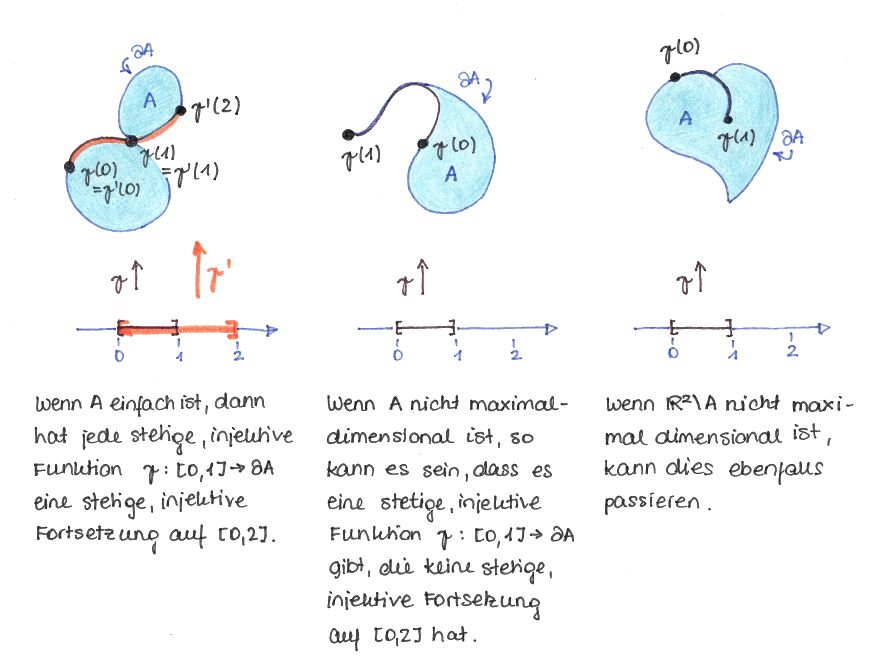
\includegraphics[width=\textwidth]{abb/rand-geht-weiter.png}
        \caption{Zu Hypothese \ref{hyp:rand-geht-weiter}}
        \label{fig:rand-geht-weiter}
    \end{figure}


%     In welchem Sinn sind einfach offene Mengen im $\R^n$ einfach? \todo{sinnvoll in den Abschnitt integrieren}
% 
%     Aus Definition \ref{def:topMet} sehen wir dass offene Teilmengen des $\R^n$ in jedem ihrer Punkte echt $n$-dimensional sind, da jeder Punkt eine ganze $\varepsilon$-Umgebung hat, die auch in der Menge liegt, man kann also von jedem Punkt aus ein Stück in jede Richtung \glqq gehen\grqq ohne die Menge zu verlassen.
%     Aus diesem Grund haben umgekehrt abgeschlossene Mengen keine niederdimensionalen Löcher. Da abgeschlossene Mengen Komplemente offener Mengen sind (Def \ref{def:CX}) ist das Komplement einer abgeschlossenen Menge überall echt $n$-dimensional.
% 
%     Wenn wir also den offene Abschluss eine Menge bilden sorgen wir durch das Abschlussbilden erst dafür, dass Löcher niederer Dimensionen verschwinden, indem wir das Innere der hierdurch entstandenen Menge nehmen schneiden wir alle niederdimensionalen Teil ab (\textcolor{red}{-> Bild}).
%     Umgekehrt werden beim abgeschlossenen Inneren erst alle Regionen der Menge entfernt, die nicht echt $n$-dimensional sind und anschließend durch den Abschluss alle niederdimensionalen Löcher.
% 
%     Dies legt nahe, dass der Rand einer einfach abgeschlossenen oder offenen Menge $n-1$-dimensional ist. Dies ist ein Frage des Dimensionsbegriffs. Man nehme Beispielsweise die Menge $M := \{(x,y) \in \R^2 \mid xy > 0\}$. Der Rand dieser Menge ist $\rand_2 M = \R \times \{0\} \cup \{0\} \times \R$ dies ist \textit{keine} 1-dimensionale topologische Mannigfaltigkeit, da es keine Umgebung des Punktes $(0,0)$ in $\rand_2 M$ gibt, die Homöomorph zu $\R$ ist.
%     

    \subsection{Ein Beispiel}\label{ssec:standardbsp}
    Die \strukt arbeitet mit einfachen Mengen auf den Rändern von einfachen Mengen.
    Das in Bsp.~\ref{bsp:standardbsp} eingeführte Standardbeispiel zeigt einige unerwartete Auswirkungen der Teilraumtopologie für die Einfachheit von Mengen.
    Insofern lassen sich mit seiner Hilfe möglicherweise problematische Beispiele für die im nächsten Kapitel definierten Repräsentanten konstruieren.
    Deshalb möchte ich dieses Beispiel hier näher untersuchen.
    
    \begin{erin}\ \\
    Aus dem vorherigen Kapitel kennen wir folgende Eigenschaften der Menge %$A$ 
    \begin{align*}
        A = \bigcup_{n \in \N} [2^{-2n}, 2^{-2n+1}]
    \end{align*}
    aus Beispiel~\ref{bsp:standardbsp}:
    %
        \begin{enumerate}
%             \item Die Menge $A$ aus Bsp.~\ref{bsp:standardbsp} ist definiert als
%                 \begin{align*}
%                     A := \bigcup_{n \in \N} [2^{-2n}, 2^{-2n+1}].
%                 \end{align*}
            \item Ihr Rand, Abschluss und Kern sind gegeben durch
                \begin{align*}
                    \rand A &= \{\frac{1}{2^n} \mid n \in \N\} \cup \{0\}\\
                    \cl(A) &= A \cup \{0\}\\
                    \op(A) &= \bigcup_{n \in \N} (2^{-2n}, 2^{-2n+1}).
                \end{align*}
            \item Für Mengen $M$ auf dem Rand von $A$ gilt:
                \begin{itemize}
                    \item $M$ ist abgeschlossen, falls es die $0$ enthält oder \textit{keine} Häufungspunkte hat.
                    \item $M$ ist offen, falls es die $0$ \textit{nicht} enthält oder $\rand A \setminus M$ \textit{keine} Häufungspunkte hat.
                \end{itemize}
            \item Sowohl $A$ als auch $\R \setminus A$ haben $0$ als Häufungspunkt.
            \item $\rand A$ hat $0$ als einzigen Häufungspunkt.
        \end{enumerate}
    \end{erin}
    
    \noindent
    Wie
    \marginpar{Einfachheit von $A$}
    sieht es mit der Einfachheit von $A$ aus?
    Es gelten:
    \begin{align*}
        &\cl(\op(\cl(A))) 
        = \cl(\op(A \cup \{0\})) 
        \\
        &\quad = \cl(\op(\bigcup_{n \in \N} [2^{-2n}, 2^{-2n+1}] \cup \{0\})) 
        = \cl(\bigcup_{n \in \N} (2^{-2n}, 2^{2n+1})) 
        \\
        &\quad = \bigcup_{n \in \N} [2^{-2n}, 2^{-2n+1}] \cup \{0\} 
        = A \cup \{0\} 
        = \cl(A)
        \\
        &\op(\cl(\op(A))) 
        = \op(\cl(\bigcup_{n \in \N} (2^{-2n}, 2^{-2n+1})))
        \\
        &\quad = \op(\bigcup_{n \in \N} [2^{-2n}, 2^{-2n+1}] \cup \{0\})
        = \bigcup_{n \in \N} (2^{-2n}, 2^{-2n+1})
        \\
        &\quad = \op(A).
    \end{align*}
    Deshalb ist $\cl(A)$ einfach abgeschlossen und $\op(A)$ einfach offen. 
    Nach Satz~\ref{satz:alt-def-einf-2} ist $A$ also einfach.\\ 
    \vspace{-5pt}
    
    \noindent
    Welche
    \marginpar{einfach abgeschlossene/offene Mengen auf dem Rand von $A$}
    Mengen auf dem Rand von $A$ einfach abgeschlossen bzw.\ offen oder auch keines von beidem sind, hängt nur von 3 Faktoren ab:
    \begin{enumerate}
        \item Ist $0$ in $B$?
        \item Hat $B$ einen Häufungspunkt?
        \item Hat $\rand A \setminus B$ einen Häufungspunkt?
    \end{enumerate}
    \noindent
    Da $\rand A$ einen Häufungspunkt bei $0$ hat, muss mindestens eine der Mengen $B$ oder $\rand A \setminus B$ dort auch einen Häufungspunkt haben.
    Deshalb gibt es nur noch 6 mögliche Fälle, die in Abbildung \ref{fig:tab-standardbsp} dargestellt sind.
    
    \begin{figure}[ht]
        \centering
        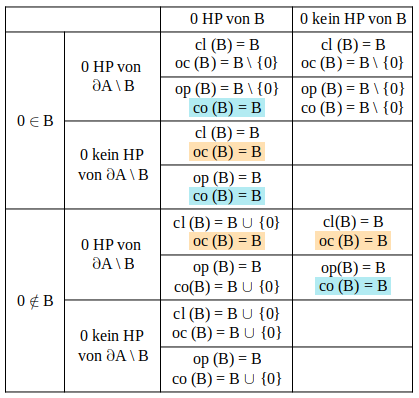
\includegraphics[width=0.7\textwidth]{abb/tab-standardbsp.png}
        \caption{Innerer Abschluss und abgeschlossenes Inneres für verschiedene Teilmengen auf $\rand A$}
        \label{fig:tab-standardbsp}
    \end{figure}
    
%     \vspace{8pt}
    
%     \noindent
%     \small
%     %\begin{tabularx}{\textwidth}{| p{1cm} | c | c | c | c |}
%     \begin{tabularx}{14.3cm}{| p{1cm} | c | c | c | c |}
%         \hline
%         & \multicolumn{2}{c |}{$0 \in B$} & \multicolumn{2}{c |}{$0 \notin B$}\\
%         \cline{2-5}
%         & $0$ HP von $B$ & $0$ nicht HP von $B$ & $0$ HP von $B$ & $0$ nicht HP von $B$\\
%         \hline
%         %\multirow{4}{*}{0 HP von \newline $\rand A \setminus B$}
%         \parbox[t]{2mm}{\multirow{4}{*}{\rotatebox[origin=c]{90}{\makecell{$0$ HP von\\$\rand A \setminus B$}}}}
%             & $\cl(B) = B$
%             & $\cl(B) = B$
%             & $\cl(B) = B \cup \{0\}$
%             & $\cl(B) = B$
%             \\
%             & $\oc(B) = B \setminus \{0\}$
%             & $\oc(B) = B \setminus \{0\}$
%             & $\oc(B) = B$
%             & $\oc(B) = B$
%             \\ \cline{2-5}
%             & $\op(B) = B \setminus \{0\}$
%             & $\op(B) = B \setminus \{0\}$
%             & $\op(B) = B$
%             & $\op(B) = B$
%             \\
%             & $\co(B) = B$
%             & $\co(B) = B \setminus \{0\}$
%             & $\co(B) = B \cup \{0\}$
%             & $\co(B) = B$\\
%         \hline
%         %\multirow{4}{*}{0 HP von \newline $\rand A \setminus B$}
%         %\multirow{4}{*}{\makecell{0 HP von \\ $\rand A \setminus B$}}
%         \parbox[t]{2mm}{\multirow{4}{*}{\rotatebox[origin=c]{90}{\makecell{$0$ kein \\ HP von \\ $\rand A \setminus B$}}}}
%             & $\cl(B) = B$
%             & 
%             & $\cl(B) = B \cup \{0\}$
%             & 
%             \\
%             & $\oc(B) = B$
%             & 
%             & $\oc(B) = B \cup \{0\}$
%             & 
%             \\ \cline{2-5}
%             & $\op(B) = B$
%             & 
%             & $\op(B) = B$
%             & 
%             \\
%             & $\co(B) = B$
%             & 
%             & $\co(B) = B \cup \{0\}$
%             & \\
%         \hline
%     \end{tabularx}
%     \vspace{8pt}
%     \normalsize
    
    \noindent
    Damit sind in $\rand A$ Teilmengen $B$
    \begin{itemize}
        \item einfach abgeschlossen, falls $0$ in $B$ und ein Häufungspunkt von $B$ oder falls $0$ \textit{nicht} in $B$ und \textit{kein} Häufungspunkt von $B$ ist
        \item einfach offen, falls $0$ in $B$ und \textit{kein} Häufungspunkt von $\rand A \setminus B$ oder falls $0$ \textit{nicht} in $B$ und ein Häufungspunkt von $\rand A \setminus B$ ist.
    \end{itemize}
    %\end{bsp}
    
    \noindent
    Mit
    \marginpar{Einfachheit von Mengen und Teilraumtopologie}
    Hilfe der Menge $A$ können wir zeigen, dass es durchaus einen Unterschied für die Einfachheit von Mengen macht, auf dem Rand welcher einfachen Mengen sie liegen.
    Mit anderen Worten: Es kann einfache Mengen $A_1$ und $A_2$ geben und eine Menge, die einfach ist in $\rand A_1$, nicht jedoch in $\rand A_2$.

    \begin{bsp}
         Seien $A_1 := [0,1]$, $A_2 := \cl(A)$.
         Es gilt: sowohl $A_1$ als auch $A_2$ sind einfach abgeschlossen in $\R$. 
         Die Menge $B := \{0\}$ ist dann einfach abgeschlossen und einfach offen in $\rand A_1$, nicht jedoch in $\rand A_2$.
         Dort ist sie nicht einmal einfach, denn $\op_{\rand A_2} (B) = \varnothing$. D.\,h.\ $\co_{\rand A_2}(B) = \varnothing$ und somit keine Obermenge von $B$. Folglich ist nach Satz~\ref{satz:alt-def-einf-2} $B$ nicht einfach in $\rand A_2$.
    \end{bsp}

    
                            %%%%%%%%%%%%%%%%%%%%%%%%%%
                          %%%                        %%%
%%%%%%%%%%%%%%%%%%%%%%%%%%%    Spezielle Randpunkte    %%%%%%%%%%%%%%%%%%%%%%%%%%%%%%%%%%
                          %%%                        %%%
                            %%%%%%%%%%%%%%%%%%%%%%%%%%
    
\section{Äußerer Rand}\label{sec:aeusserer-rand}

    Einfache
    \marginpar{Probleme mit den Rändern einfacher Mengen}
    Mengen sind mit weiteren Einschränkungen die Kandidaten für Raumregionen. Euklidische Flächen sind einfache Mengen auf dem Rand einfacher Mengen.
    Nicht jede einfache Teilmenge des Randes jeder einfachen Teilmenge eignet sich jedoch als euklidische Fläche im Sinne der Theorie $\theoryBSO$, wie folgendes, um eine Dimension reduziertes Beispiel verdeutlicht:
    
    \begin{gegenbsp}\label{gegenbsp:aeusserer-rand}
        Seien $A := \{(x,y) \in \R^2 \mid xy \geq 0\}$, $B := [-1,1] \times \{0\}$ und $p := (0,0)$. 
        %Dann sind $A \in \CO(\R^2)$, $B \in \CO(\rand A)$ und $p \in \rand_{\rand A}B$.
        Dann sind $A \in \CO(\R^2)$ und $B \in \CO(\rand A)$.
        Somit ist $p$ ein Randpunkt von $B$ in $\rand A$, denn $\rand A$ besteht aus der $x$- und der $y$-Achse und in jeder Umgebung von $p$ in $\rand A$ liegen sowohl Punkte der $x$-Achse, die im Inneren von $B$ sind, als auch Punkte der $y$-Achse, die nicht in $B$ sind (siehe Abbildung \ref{fig:kein-aeusserer-rand}).
        Allerdings eignet sich $p$ nicht als Grenzpunkt von $B$, denn für $p$ lässt sich nicht eindeutig eine Richtung festlegen, \glqq aus der die durch $p$ begrenzte Linie kommt\grqq, denn $B$ erstreckt sich sowohl links als auch rechts von $p$.
        Die Endpunkte $(-1,0)$ und $(1,0)$ von $B$ hingegen bezeichne ich als äußeren Rand.
    \end{gegenbsp}
    
    \begin{figure}[ht]
        \centering
        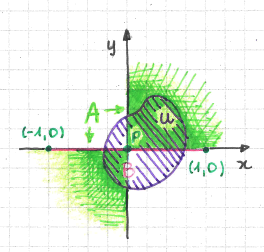
\includegraphics[width=5cm]{abb/kein-aeusserer-rand.png}
        %\caption[Kein äußerer Randpunkt]{Zu Gegenbeispiel \ref{gegenbsp:aeusserer-rand}}
        \caption{Zu Gegenbeispiel \ref{gegenbsp:aeusserer-rand}}
        \label{fig:kein-aeusserer-rand}
    \end{figure}

    Die
    \marginpar{äußerer Rand}folgende Definition formalisiert diese intuitive Vorstellung des äußeren Randes.
    Vereinfacht gesagt ist ein äußerer Randpunkt einer einfachen Menge, die auf dem Rand einer anderen einfachen Menge \glqq lebt\grqq, ein Punkt, der immer Randpunkt ist, egal, wie diese andere einfache Menge genau aussieht.

    \begin{dfn}[Äußerer Rand]\label{def:aeusserer-rand} \ \vspace{8pt}

        \noindent
        Sei $X$ ein topologischer Raum.
        Seien $A \in \OC_X$, $B \in \OC_{\rand_X A}$ und $x \in \rand_{\rand_X A}(B)$. Dann ist $x$ ein äußerer Randpunkt von $B$, falls gilt
        \begin{align*}
            \forall\: A' \in \OC_X : (\: B \in \OC_{\rand_X A'} \rightarrow x \in \rand_{\rand_X A'}(B) \:)
        \end{align*}
        Die \thmemph{Menge der äußeren Randpunkte} von $B$ bezeichnen wir mit $\delta_X(B)$.\\
        Ein Punkt aus $\rand_{\rand_X A} B$, der kein äußerer Randunkt von $B$ ist, heißt \thmemph{innerer Randpunkt} von $B$ in $\rand_X A$.
    \end{dfn}


    \begin{figure}[ht]
        \centering
        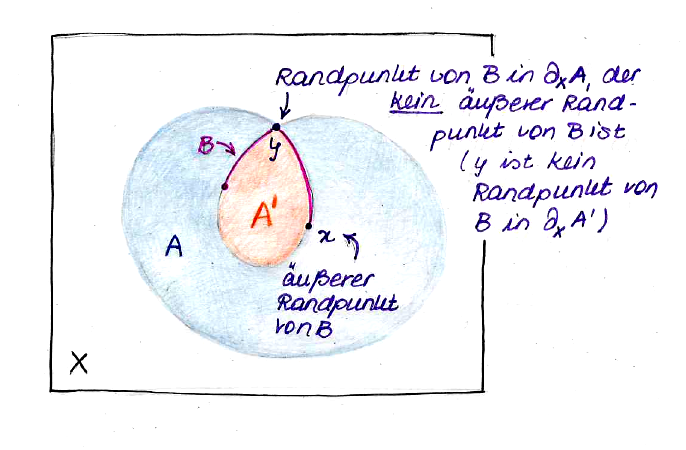
\includegraphics[height=7cm]{abb/aeusserer-rand.png}
        \caption{zu Def. \ref{def:aeusserer-rand} (äußerer Rand)}
        \label{fig:aeus-rand}
    \end{figure}
    
%     \todo[inline]{Bsp. mit Beweis. Z.B. $(0,1)$ aus Gegenbsp.}
%     \begin{bsp}\label{bsp:aeusserer-rand}
%        x
%     \end{bsp}
% 
%     Für \textcolor{red}{weitere} Beispiele und Gegenbeispiele zu äußeren Rand im $\R^3$ und auf seinen Teilmengen -- die allerdings die in Abschnitt \ref{ssec:notationelle-konv} eingeführten vereinfachten Notationen verwenden -- siehe Abbildung \ref{fig:notationen-r3}.
% 
%     \todo{Beispiele}
    
    Der
    \marginpar{äußerer rand $n$-ter Stufe}
    Begriff des äußeren Randes lässt sich verallgemeinern zum äußeren Rand $n$-ter Stufe. Hier genügt uns $n = 2$.
    
    \begin{dfn}[Äußerer Rand zweiter Stufe]\label{def:aeusserer-rand-2} \ \vspace{8pt}

        \noindent
        Sei $X$ ein topologischer Raum.
        Seien $A \in \OC_X$, $B \in \OC_{\rand_X A}$, $C \in \OC_{\delta B}$ und $x \in \rand_{\rand_{\rand_X A}(B)}(C)$. Dann ist $x$ ein äußerer Randpunkt 2.~Stufe von $C$, falls gilt
        \begin{align*}
            \forall\: A' \in \OC_X, B' \in \OC_{\rand_X A'} : (\: C \in \OC_{\delta B'} \rightarrow x \in \rand_{\rand_{\rand_X A'}(B')}(C) \:)
        \end{align*}
        Die \thmemph{Menge der äußeren Randpunkte 2. Stufe} von $C$ bezeichnen wir mit $\delta_X^2(C)$.\\
        Ein Punkt aus $\rand_{\rand_{\rand_X A}(B)}(C)$, der kein äußerer Randunkt zweiter Stufe von $C$ ist, heißt \thmemph{innerer Randpunkt} von $C$ in $\rand_{\rand_X A}(B)$.
    \end{dfn}
    
    Die Vorstellung, die dem Begriff des äußeren Randes zugrunde liegt, ist, dass es nach einem äußeren Randpunkt \glqq wirklich nicht weiter geht\grqq.
    
%     Für eine euklidische Linie $C$ sollte $p$ ein äußerer Randpunkt zweiter Stufe sein, wenn sie dort in einer \glqq Sackgasse\grqq\ landet.
%     Im anderen Fall, also wenn $C$ in $p$ keine Sackgasse hat, gibt es mindestens zwei Richtungen in $C$ in die man von $p$ aus gehen kann. 
%     Mathematisch gesprochen bedeutet dies, dass es eine stetige injektive Abbildung $\gamma:(-1,1) \to C \cup \{p\}$ gibt mit $\gamma(0) = p$.

    Im
    \marginpar{Sackgassenbild}
    $\R^2$ ist damit gemeint:
    Für eine euklidische Linie $B$ ist $p$ ein äußerer Randpunkt, wenn $B$ in $p$ eine Sackgasse hat.
    Ist dies nicht der Fall -- genauer: sind $A \in \OC_2$, $B \in \OC_{\rand A}$ und $p \in \rand_{\rand_A} B$ kein äußerer Randpunkt von $B$ -- so gibt es von $p$ aus mindestens zwei Richtungen in $B$.
    Mathematisch bedeutet dies, dass es eine stetige injektive Abbildung $\gamma:(-1,1) \to B \cup \{p\}$ gibt mit $\gamma(0) = p$.

    \begin{figure}[ht]
        \centering
        \includegraphics[height=7cm]{abb/pflasterbild-innerer-rp.png}
        \caption[Zu Hypothese \ref{hyp:aeusserer-rand} (innerer Randpunkt)]{Zu Hypothese \ref{hyp:aeusserer-rand}: Ist $p$ ein innerer Randpunkt von $B \subseteq \R^3$, so gibt es eine stetige, injektive Abbildung $f:U \to \cl_{\rand A} B$ mit $p \in f(U)$, wobei $U \in \offen_2$ ist.}
        \label{fig:pflasterbild-innerer-rp}
    \end{figure}
    
    
    Die
    \marginpar{Einbettung von $\R^{n-1}$ und innere Randpunkte}
    folgende Hypothese verallgemeinert diese Vorstellungen auf Teilmengen des $\R^n$

    \begin{figure}[ht]
        \centering
        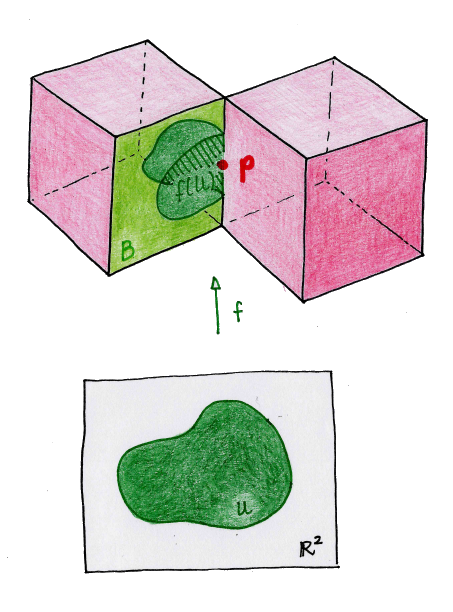
\includegraphics[height=7cm]{abb/pflasterbild-aeusserer-rp.png}
        \caption[Zu Hypothese \ref{hyp:aeusserer-rand} (äußerer Randpunkt)]{Zu Hypothese \ref{hyp:aeusserer-rand}: Ist $p$ ein äußerer Randpunkt von $B \subseteq \R^3$, so kann eine stetige Abbildung $f:U \to \cl_{\rand A} B$ mit $p \in f(U)$, wobei $U \in \offen_2$ ist, nicht injektiv sein.}
        \label{fig:pflasterbild-aeusserer-rp}
    \end{figure}
    
    \todo[inline]{Bilder zusammenfügen}


    \begin{hyp}[Äußerer Rand in $\R^n$]\label{hyp:aeusserer-rand} \ \vspace{8pt}

        \noindent
        Seien $n \in \N$ mit $n \geq 2$, $A \in \einf_{\R^n}$ und $B \in \einf_{\rand_{\R^n} A}$. Ein Punkt $p \in \rand_{\rand A}(B)$ ist genau dann ein äußerer Randpunkt von $B$, falls es \textit{keine} stetige injektive Abbildung $f : U \to \cl_{\rand A}(B)$ gibt mit $p \in f(U)$ für eine offene Menge $U \in \offen_{\R^{n-1}}$.
    \end{hyp}
    
    Diese Vorstellung gilt analog für äußere Randpunkte höherer Stufe.
    
    Die Abbildungen \ref{fig:pflasterbild-innerer-rp} und \ref{fig:pflasterbild-aeusserer-rp} illustrieren diese Hypothese für $n=3$.
    
    %Abbildung \ref{fig:pflasterbild-innerer-rp} zeigt einen inneren Randpunkt einer Teilmenge des $\R^3$, Abbildung \ref{fig:pflasterbild-aeusserer-rp} einen äußeren.
    

    
    
%     \begin{figure}
%         \begin{subfigure}{.5\textwidth}
%             \centering
%             \includegraphics[width=.8\linewidth]{pflasterbild-innerer-rp.png}
%             \caption{Ist $p$ ein innerer Randpunkt von $B \subseteq \R^3$, so gibt es eine stetige, injektive Abbildung $f:U \to \cl_{\rand A} B$ mit $p \in f(U)$, wobei $U \in \offen_2$ ist.}
%             \label{fig:aeusserer-rand-2-innen}
%         \end{subfigure}%
%         \begin{subfigure}{.5\textwidth}
%             \centering
%             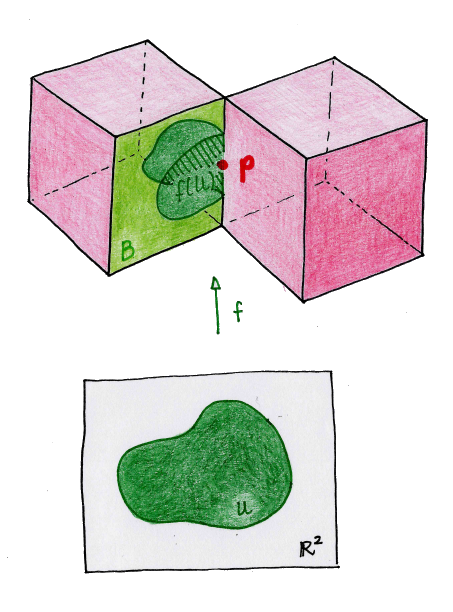
\includegraphics[width=.8\linewidth]{abb/pflasterbild-aeusserer-rp.png}
%             \caption{Ist $p$ ein äußerer Randpunkt von $B \subseteq \R^3$, so kann eine stetige Abbildung $f:U \to \cl_{\rand A} B$ mit $p \in f(U)$, wobei $U \in \offen_2$ ist, nicht injektiv sein.}
%             \label{fig:aeusserer-rand-2-aussen}
%         \end{subfigure}
%         \caption{Zu Hypothese \ref{hyp:aeusserer-rand}}
%         \label{fig:aeusserer-rand-2}
%     \end{figure}
    
    Weniger
    \marginpar{Pflasterbild}
    mathematisch als in der Bildbeschreibung, kann man die Frage, ob $p$ ein äußerer Randpunkt von $B$ im $\R^3$ ist, auf folgende zurückführen:
    Ist $B$ verletzt bei $p$, kann ich dann ein Pflaster auf $B$ kleben, das $p$ überdeckt, ohne dass ich es umklappen muss (siehe Abbildungen \ref{fig:pflasterbild-aeusserer-rand} und \ref{fig:pflasterbild-innerer-pkt})?
    
    \begin{figure}[ht]
        \centering
        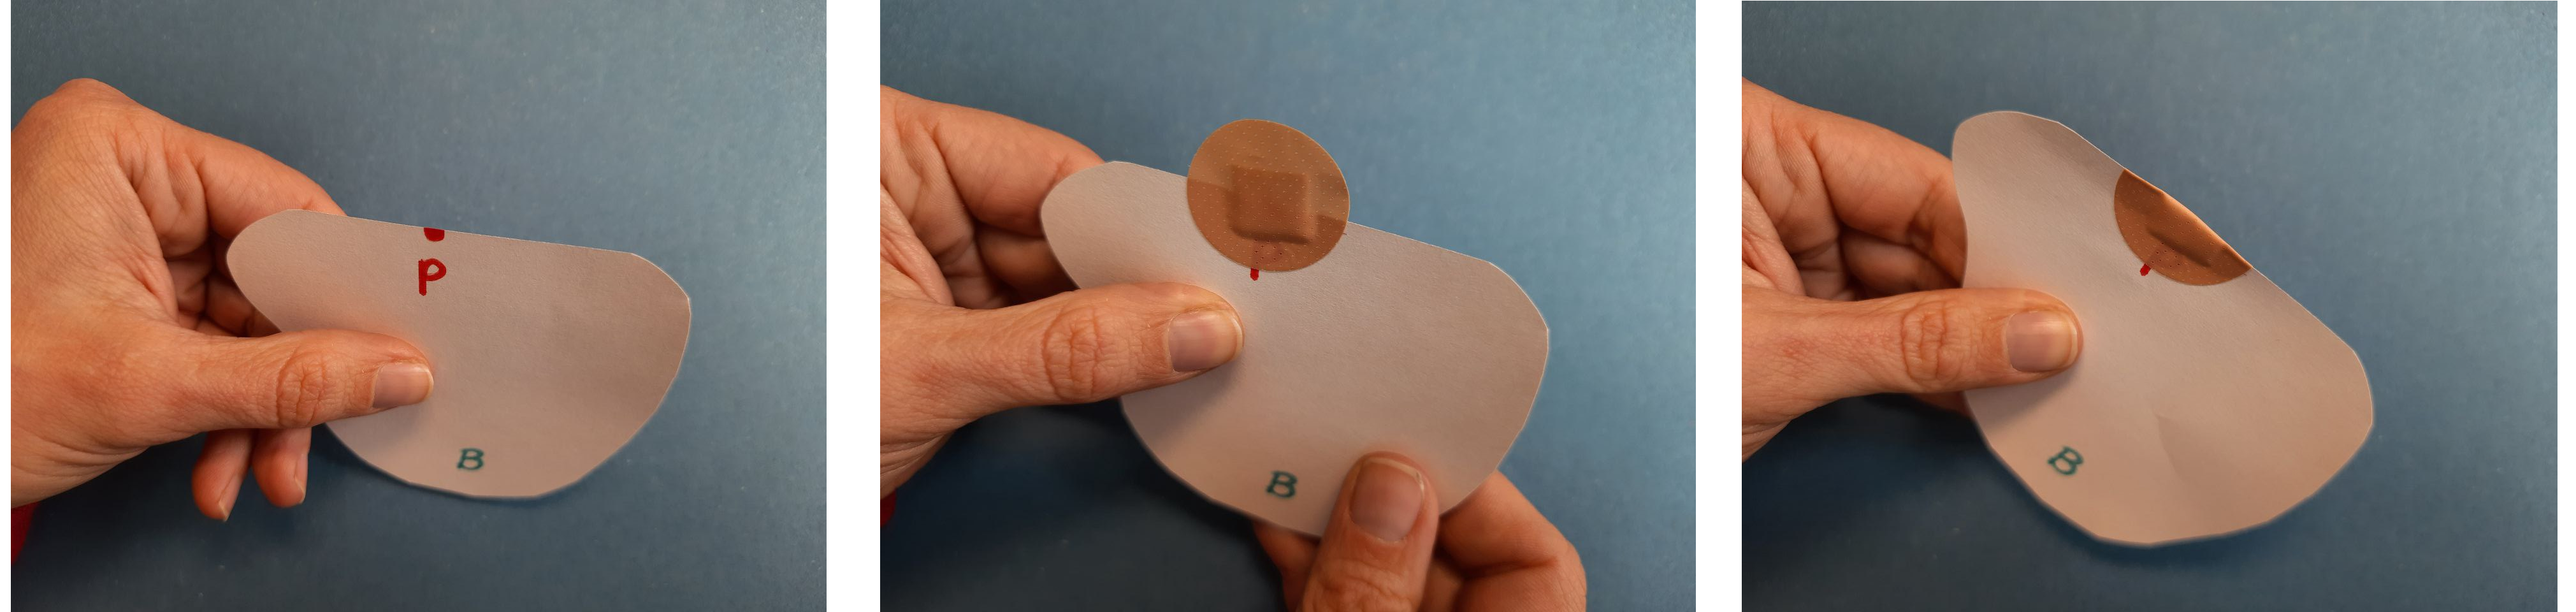
\includegraphics[width=\textwidth]{abb/pflasterbild-aeusserer-rand.png}
        \caption[Pflasterbild: äußerer Randpunkt]{Pflasterbild: Wenn $p$ ein äußerer Randpunkt einer Fläche $B$ ist, so kann ich kein Pflaster auf $B$ kleben, das $p$ überdeckt, ohne dass ich es umklappen muss.}
        \label{fig:pflasterbild-aeusserer-rand}
    \end{figure}
    
    \begin{figure}[ht]
        \centering
        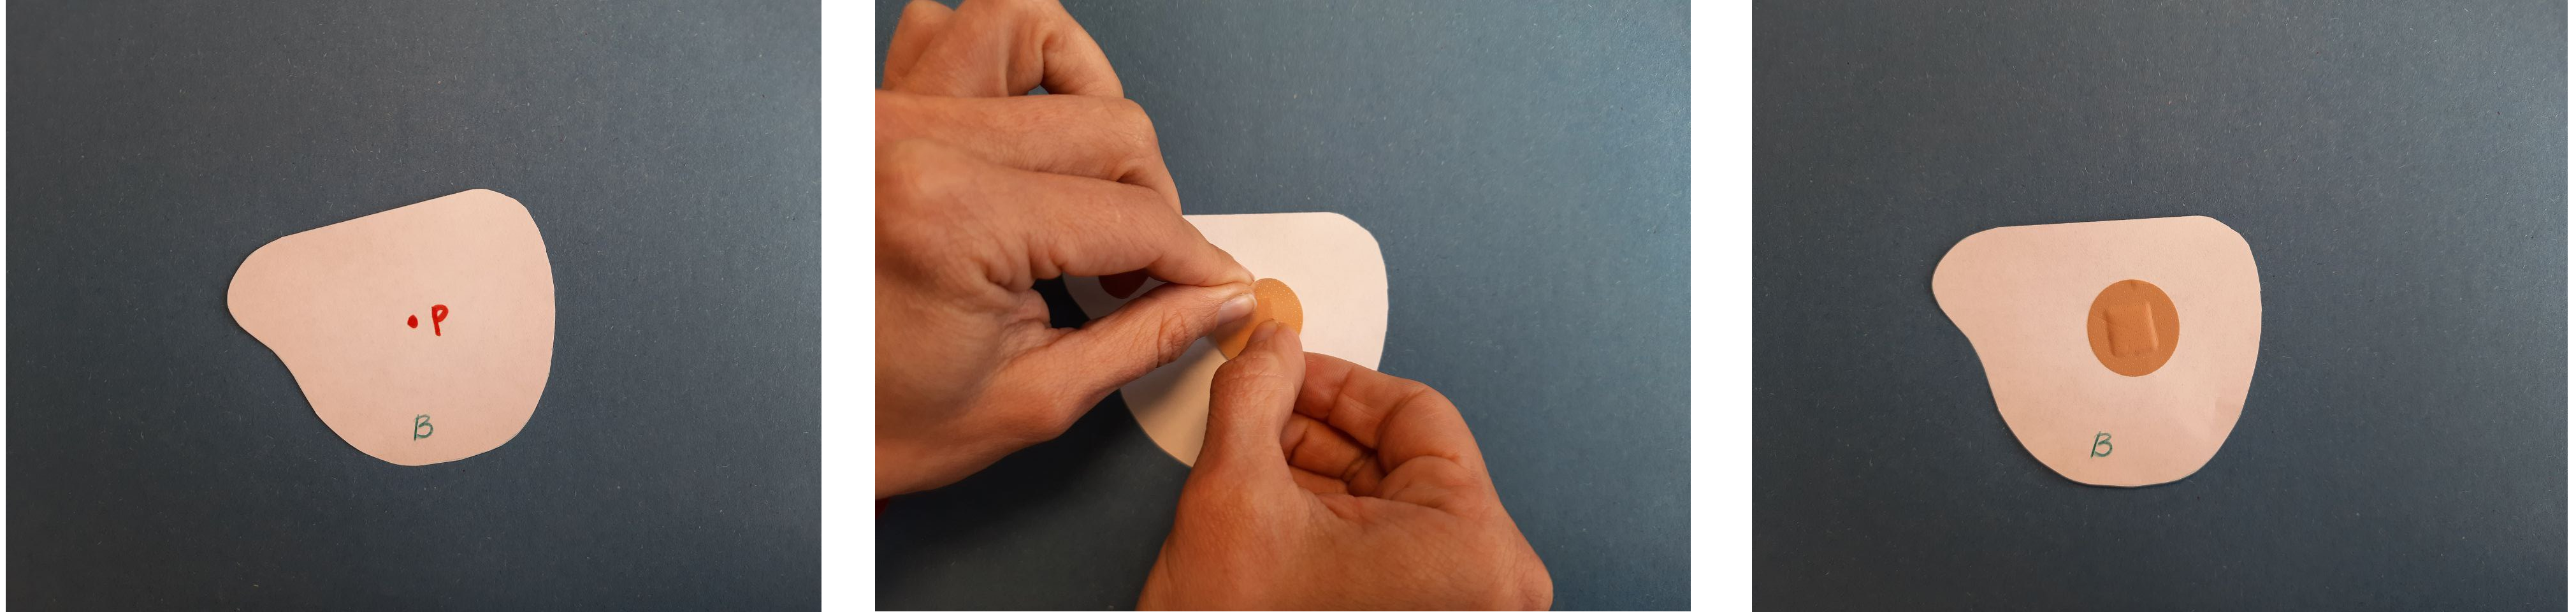
\includegraphics[width=\textwidth]{abb/pflasterbild-innerer-pkt.png}
        \caption[Pflasterbild: innerer Punkt]{Pflasterbild: Wenn $p$ ein innerer (Rand)Punkt einer Fläche $B$ ist, so kann ich ein Pflaster auf $B$ kleben, das $p$ überdeckt, ohne es umzuklappen.}
        \label{fig:pflasterbild-innerer-pkt}
    \end{figure}
    
%    \textcolor{white}{xx}

\bigskip
\todo[inline]{FL: bitte Überleitungstext prüfend lesen; ein paar überleitende Sätze sollte es m.E. hier geben\\
-> BH: Danke, der Text ist gut und bindet die Arbeit besser zusammen.}
Mit dem äußeren Rand sowie den eingangs in diesem Kapitel eingeführten Konzepten der lokalen Gleichheit und insbesondere der einfachen Mengen sind nun zusätzliche topologische Grundlagen geschaffen. Darauf aufbauend können die Entwicklungslinien aus den vorstehenden Kapiteln dieser Arbeit in deren sich nun anschließendem dritten Teil zusammengeführt werden, um die bislang grundlegend entworfene Interpretation für die Axiomatisierung $\theoryBSO$ in der angestrebten Art und Weise weiter zu entwickeln und auf ihre Zweckmäßigkeit für den Nachweis der Konsistenz der Theorie hin zu untersuchen.

    

                            %%%%%%%%%%%%%%%%%%%%%%%%%%%%%%%
                          %%%                             %%%
%%%%%%%%%%%%%%%%%%%%%%%%%%%    Notationelle Konventionen    %%%%%%%%%%%%%%%%%%%%%%%%%%%%%%%%%%
                          %%%                             %%%
                            %%%%%%%%%%%%%%%%%%%%%%%%%%%%%%%
    
% \section{Notationelle Konventionen auf $\R^3$}\label{ssec:notationelle-konv}
% Da der hier vorgestellte Interpretationsansatz für $\BS^O$ auf einfach abgeschlossenen Mengen, derer Rändern und deren äußeren Rändern arbeitet, führe ich hierfür vereinfachte Notationen ein. Abbildung \ref{fig:notationen-r3} zeigt die eingeführten Konventionen an ausgewählten Beispielen.
% 
% \begin{figure}[ht]
%     \centering
%     \includegraphics[height=7cm]{abb/notationen-r3.png}
%     \caption{Beispiele und Gegenbeispiele zum äußeren Rand mit vereinfachter Notation}
%     \label{fig:notationen-r3}
% \end{figure}
% 
% \begin{konv}[Topologische Notationen auf $\R^3$]\ \vspace{8pt}
% 
% \noindent 
%     Im $\R^3$ vereinfachen wir die topologischen Notationen für
%     \begin{enumerate}
%     	\item die \thmemph{Topologie} $\offen_{\R^3}$ durch $\offen$
%     	\item den \thmemph{Abschlussoperator} $\cl_{\R^3}$ durch $\cl$
%     	\item den \thmemph{Kernoperator} $\op_{\R^3}$ durch $\op$
%     	\item den \thmemph{$\boldsymbol{\co}$-Operator} $\co_{\R^3}$ durch $\co$
%     	\item den \thmemph{$\boldsymbol{\oc}$-Operator} $\oc_{\R^3}$ durch $\oc$
%     	\item den \thmemph{Randoperator} $\rand_{\R^3}$ durch $\rand$
%     	%\item den \thmemph{echten Randoperator} $\Delta_{\R^3}$ durch $\Delta$
%     	\item den \thmemph{äußeren Randoperator} $\delta_{\R^3}$ durch $\delta$
%     	\item die \thmemph{Menge der einfachen Mengen} $\einf_{\R^3}$ durch $\einf$
%     	\item die \thmemph{Menge der einfach abgeschlossenen Mengen} $\CO_{\R^3}$ durch $\OC$
%     	\item die \thmemph{Menge der einfach offenen Mengen} $\OC_{\R^3}$ durch $\OC$
%     \end{enumerate}
%     
% %    \noindent
% %    Für $A \subseteq \R^3$ schreiben wir auch $\rand A$ statt $\rand (A)$.
% 
% \end{konv}
% 
% 
% \begin{konv}[Topologische Notationen auf $\rand A$]\ \vspace{8pt}
% 
% \noindent 
%     Für $A \in \CO$ vereinfachen wir die topologischen Notationen auf $\rand A$ für
%     \begin{enumerate}
%     	\item die \thmemph{Topologie} $\offen_{\rand A}$ durch $\offen_A$
%     	\item den \thmemph{Abschlussoperator} $\cl_{\rand A}$ durch $\cl_A$
%     	\item den \thmemph{Kernoperator} $\op_{\rand A}$ durch $\op_A$
%     	\item den \thmemph{$\boldsymbol{\co}$-Operator} $\co_{\rand A}$ durch $\co_A$
%     	\item den \thmemph{$\boldsymbol{\oc}$-Operator} $\oc_{\rand A}$ durch $\oc_A$
%     	\item den \thmemph{Randoperator} $\rand_{\rand A}$ durch $\rand_A$
%     	%\item den \thmemph{echten Randoperator} $\Delta_{\Delta A}$ durch $\Delta_A$
%     	\item den \thmemph{äußeren Randoperator} $\delta_{\rand A}$ durch $\delta_A$
%     	\item die \thmemph{Menge der einfachen Mengen} $\einf_{\rand A}$ durch $\einf_A$
%     	\item die \thmemph{Menge der einfach abgeschlossenen Mengen} $\CO_{\rand A}$ durch $\CO_A$
%     	\item die \thmemph{Menge der einfach offenen Mengen} $\OC_{\rand A}$ durch $\OC_A$
%     \end{enumerate}
% 
% \end{konv}
% 
% 
% % \begin{konv}[Topologische Notationen auf $\delta(B)$]\ \vspace{8pt}
% % 
% % \noindent 
% %     Für $A \in \CO$ und $B \in \CO_A$ vereinfachen wir die topologischen Notationen auf $\delta B$ für
% %     \begin{enumerate}
% %     	\item die \thmemph{Topologie} $\offen_{\Delta_A(B)}$ durch $\offen_{A,B}$
% %     	\item den \thmemph{Abschlussoperator} $\cl_{\Delta_A(B)}$ durch $\cl_{A,B}$
% %     	\item den \thmemph{Kernoperator} $\op_{\Delta_A(B)}$ durch $\op_{A,B}$
% %     	\item den \thmemph{$\boldsymbol{\co}$-Operator} $\co_{\Delta_A(B)}$ durch $\co_{A,B}$
% %     	\item den \thmemph{$\boldsymbol{\oc}$-Operator} $\oc_{\Delta_A(B)}$ durch $\oc_{A,B}$
% %     	\item den \thmemph{Randoperator} $\rand_{\Delta_A(B)}$ durch $\rand_{A,B}$
% %     	\item den \thmemph{echten Randoperator} $\Delta_{\Delta_A(B)}$ durch $\Delta_{A,B}$
% %     	\item den \thmemph{äußeren Randoperator} $\delta_{\Delta_A(B)}$ durch $\delta_{A,B}$
% %     	\item die \thmemph{Menge der einfach abgeschlossenen Mengen} $\CO_{\Delta_A(B)}$ durch $\CO_{A,B}$
% %     	\item die \thmemph{Menge der einfach offenen Mengen} $\OC_{\Delta_A(B)}$ durch $\OC_{A,B}$
% %     \end{enumerate}
% % 
% % \end{konv}
% 

% 
% %\part{Die \strukt}
% \part{Zusammenführung}
% 
% %\chapter{Eine Interpretation für die Theorie $\theoryBSO$}\label{chap:bso-struktur}
\chapter{Formale Definition der \strukt}\label{chap:bso-struktur}
    In Kapitel \ref{chap:bso-grundideen} habe ich die \strukt als Interpretation von $\theoryBSO$ eingeführt, wobei die genauen Definitionen der Repräsentanten und der Objektäquivalenz offen gelassen wurden. 
    Mit Hilfe der im vorangegangenen Kapitel~\ref{chap:topologie-erweiterung} neu eingeführten topologischen Begriffe werden diese Lücken in Abschnitt \ref{sec:univ-2} geschlossen.
    Der Abschnitt~\ref{sec:analyse} reißt die Fragen an, ob der vorgeschlagene Ansatz die Vorstellungen, die mit der Theorie verbunden sind adäquat wiederspiegelt und ob er ein Modell von $\theoryBSO$ ist, kann diese jedoch nicht abschließend beantworten.
% 
%     Da im Rahmen dieser Arbeit weder ausführlich untersucht werden kann, ob der vorgeschlagene Ansatz die Vorstellungen, die mit der Theorie verbunden sind adäquat wiederspiegelt, noch, ob er ein Modell von $\theoryBSO$ ist, werden diese beiden Fragen in Abschnitt~\ref{sec:analyse} zumindest an einigen Beispielen untersucht

% --------------------------------------------------------------------------------------

    \section{Repräsentanten und Objektäquivalenz}\label{sec:univ-2}
    In diesem Abschnitt stelle ich die in \ref{sec:ausblick} angekündigten Definitionen für Raumregionen, Repräsentanten und die Objektäquivalenz der \strukt bereit.
    
%     \begin{erin}[Eigenschaften von Raumregionen]\ \vspace{0pt}
%         \begin{itemize}
%             \item[(R0)] Raumregionen sind beschränkt.
%             \item[(R1)] Sie sind überall echt 3-dimensional (insbesondere enthalten sie keine niederdimensionalen Ausläufer).
%             \item[(R2)] Ihr Rand ist überall echt 2-dimensional.
%             \item[(R3)] Sie enthalten keine niederdimensionalen Löcher.
%         \end{itemize}
%     \end{erin}
%     

    Zur Erinnerung: Raumregionen sind Teilmengen des $\R^3$, die überall echt 3-dimensional sind und einen 2-dimensionalen Rand haben.%
    \marginpar{Raumregionen}
    Mit Hilfe des in ~\ref{sec:einf-mengen} eingeführten Begriffs der einfach offenen Menge definiere ich nun:
    
    \begin{dfn}[Raumregion]\ \\
        Eine Teilmenge $A \subseteq \R^3$ heißt Raumregion, wenn
        \begin{enumerate}
            \item $\varnothing \neq A \in \OC$ und
            \item $A$ beschränkt%  
                  \footnote{Eine Teilmenge $A \subseteq \R^n$ ist beschränkt falls $\exists\: M \in \R : A \subseteq B_M(0)$.}
                  ist
        \end{enumerate}
        Die Menge der Raumregionen bezeichnen wir mit $\univ^3$
    \end{dfn}
    Ob dieser Ansatz alle Vorstellung adäquat wiederspiegelt, die mit dem Begriff der Raumregion verbunden sind, ob also einfache Mengen alle gewünschten Eigenschaften besitzen, ist eine mathematisch anspruchsvolle Frage, die hier nicht abschließend geklärt werden kann. Sie wird in \ref{chap:diskussion} noch weiter ausgeführt.
    
    \begin{bsp}[$\varepsilon$-Bälle als Raumregionen]\ \\
        Für jedes $x \in \R^3$ und jedes $\varepsilon > 0$ ist $B_\varepsilon(x)$ eine Raumregion.
    \end{bsp}
    
    
    Niederdimensionale Raumentitäten werden als Äquivalenzklassen von Repräsentanten betrachtet.
    Diese Repräsentanten sind Tupel von euklidischen Entitäten.%
    \marginpar{euklidische Entitäten,\\Repräsentanten}
    Kurz gesagt sind euklidische Entitäten Teilmengen des $\R^3$, die auf den Rändern von höherdimensionalen euklidischen Entitäten liegen und deren Ränder Kodimension 1 haben.
    Genauer gesagt: 3-dimensionale euklidische Entitäten sind Raumregionen.
    $n$-dimensionale euklidische Entitäten liegen auf den Rändern von $(n+1)$-dimensionalen und haben einen $(n-1)$-dimensionalen Rand.
    Auf die explizite Definition dieser Entitäten kann ich hier verzichten, denn sie ergibt sich im Nachhinein aus der Definition der Repräsentanten.

    \begin{dfn}[Repräsentanten]\label{dfn:repr}\ \vspace{0pt}

        \begin{enumerate}
            \item $(A,B)$ ist ein \spacedlowsmallcaps{Flächenrepräsentant}, wenn 
                \begin{enumerate}
                    \item $A$ eine Raumregion und
                    \item $\varnothing \neq B \in \OC_{\rand A}$ ist.
                \end{enumerate}
                Die \spacedlowsmallcaps{Menge der Flächenrepräsentanten} bezeichnen wir mit $\rep^2$
            \item $(A,B,C)$ ist ein \spacedlowsmallcaps{Linienrepräsentant}, wenn 
                \begin{enumerate}
                    \item $(A,B)$ ein Flächenrepräsentant und
                    \item $\varnothing \neq C \in \OC_{\delta B}$ ist.
                \end{enumerate}
                Die \spacedlowsmallcaps{Menge der Linienrepräsentanten} bezeichnen wir mit $\rep^1$
            \item $(A,B,C,D)$ ist ein \spacedlowsmallcaps{Punktrepräsentant}, wenn 
                \begin{enumerate}
                    \item $(A,B,C)$ ein Linienrepräsentant und
                    \item $D \subseteq \delta^2 C$ ist.
                \end{enumerate}
                Die \spacedlowsmallcaps{Menge der Punktrepräsentanten} bezeichnen wir mit $\rep^0$
        \end{enumerate}
    %	
    \end{dfn}
    
    Für die so definierten Repräsentanten ergibt sich trivialerweise:
    
    \begin{satz}\ \vspace{0pt}
    
        \begin{itemize}
            \item Für jede Raumregion $A$ gilt: $(A, \rand A)$ ist ein Flächenrepräsentant.
            \item Für jeden Flächenrepräsentanten $(A,B)$ gilt: 
                Falls $\delta B \neq \varnothing$ ist, ist $(A, B, \delta B)$ ein Linienrepräsentant.
            \item Für jeden Linienrepräsentanten $(A,B,C)$ gilt: 
                Falls $\delta^2 C \neq \varnothing$ ist, ist $(A, B, C, \delta^2 C)$ ein Punktrepräsentant.
        \end{itemize}
        
    \end{satz}
    
    
    Die Objektäquivalenz erfasst in geeigneter Weise, was es heißt, dass zwei Raumentitäten \glqq von der gleichen Seite\grqq\ bzw.\ \glqq aus der gleichen Richtung\grqq\ auf eine dritte zukommen. 
    \marginpar{Objektäquivalenz}
    Hier erweist sich der in Abschnitt~\ref{sec:lokale-gleichheit} definierte Begriff der lokalen Gleichheit als hilfreich.

    \begin{dfn}[Objektäquivalenz, $\sim$]\label{dfn:objektaequivalenz}\ \vspace{0pt}

        \begin{enumerate}
            \item Zwei \spacedlowsmallcaps{Flächenrepräsentanten} $(A_1,B_1)$ und $(A_2,B_2)$ sind \spacedlowsmallcaps{objektäquivalent}, wenn 
                \begin{enumerate}
                    \item $B_1 = B_2$ und
                    \item $A_1 =_{B_1} A_2$
                \end{enumerate}
                gelten
            \item Zwei \spacedlowsmallcaps{Linienrepräsentanten} $(A_1,B_1,C_1)$ und \\
            $(A_2,B_2,C_2)$ sind \spacedlowsmallcaps{objektäquivalent}, wenn 
                \begin{enumerate}
                    \item $C_1 = C_2$,
                    \item $A_1 =_{C_1} A_2$ und $B_1 =_{C_1} B_2$
                \end{enumerate}
                gelten.
            \item Zwei \spacedlowsmallcaps{Punktrepräsentanten} $(A_1,B_1,C_1,D_1)$ und\\
                $(A_2,B_2,C_2,D_2)$ sind \spacedlowsmallcaps{objektäquivalent}, wenn 
                \begin{enumerate}
                    \item $D_1 = D_2$,
                    \item $A_1 =_{D_1} A_2$, $B_1 =_{D_1} B_2$ und $C_1 =_{D_1} C_2$
                \end{enumerate}	
                gelten.		
        \end{enumerate}
        
        Wenn zwei Repräsentanten $x$ und $y$ objektäquivalent sind, so schreiben wir $x \sim y$.
        
    \end{dfn}
    
    Bei der informellen Einführung der Objektäquivalenz in Abschnitt~\ref{sec:universum} wurde die Äquivalenzrelationseigenschaft gefordert, die nun auch nachgewiesen werden kann.
    
    \begin{satz}\ \\
        Die Objektäquivalenz ist eine Äquivalenzrelation auf\\
        $\rep^2 \cap \rep^1 \cap \rep^0$.
    \end{satz}
    
    Beweis: Direkte Folgerung aus Korollar \ref{kor:lokale-gleichheit-aer} (die lokale Gleichheit bzgl. einer festen Menge ist eine Äquivalenzrelation) und der Äquivalenzrelationseigenschaft von \glqq = \grqq .
 
 
    
%-----------------------------------------------------------------------------
    
    
    
%     \section{Universum und primitive Relationen in der \strukt}
% 
%     
%     - Übersicht 3
%     - Wie wirken sich die neuen Definitionen auf das Universum und die primitiven Relationen aus?
% 
%     
%     \begin{erin}[Flächen-, Linien- und Punktregionen] \ \vspace{0pt}
% 
%         \noindent
%             Sei $\sim$ eine Objektäquivalenz.
%             
%             \begin{enumerate}
%         			
%                 \item Für $(A,B) \in \rep^2$ bezeichnet 
%                     \begin{align*}
%                         [A,B] := \{(A',B') \in \rep^2 \mid (A',B') \sim (A,B)\}
%                     \end{align*}
%                     die Äquivalenzklasse von $(A,B)$ bezüglich der Objektäquivalenz.\\
%                     Diese Äquivalenzklassen heißen \spacedlowsmallcaps{Flächenregionen}.
%                     
%                 \item Für $(A,B,C) \in \rep^1$ bezeichnet
%                     \begin{align*}
%                         [A,B,C] := \{(A',B',C') \in \rep^1 \mid (A',B',C') \sim (A,B,C)\}
%                     \end{align*}			 
%                     die Äquivalenzklasse von $(A,B,C)$ bezüglich der Objektäquivalenz.\\
%                     Diese Äquivalenzklassen heißen \spacedlowsmallcaps{Linieregionen}.
%         			
%                 \item Für $(A,B,C,D) \in \rep^0$ bezeichnet
%                     \begin{align*}
%                         &[A,B,C,D] := \\
%                         &\{(A',B',C',D') \in \rep^0 \mid (A',B',C',D') \sim (A,B,C,D)\}
%                     \end{align*}			 
%                     die Äquivalenzklasse von $(A,B,C,D)$ bezüglich der Objektäquivalenz.\\
%                     Diese Äquivalenzklassen heißen \spacedlowsmallcaps{Punktregionen}.
%         			
%             \end{enumerate}
%             
%             \noindent	
%                 Für $i \in \{0,1,2\}$ ist $\univ^i := \rep^i /_\sim$ die \spacedlowsmallcaps{Menge der Äquivalenzklassen} von $\rep^i$.\\
%                 $\univ^3$ ist die \spacedlowsmallcaps{Menge der Raumregionen}.\\
%                 $\univ := \univ^3 \cup \univ^2 \cup \univ^1 \cup \univ^0$ ist das \spacedlowsmallcaps{Universum} der \strukt.
%         
%     \end{erin}
%     
%     \begin{erin}[Universum]\ \vspace{8pt}
% 
%         \noindent
%         Das Universum der \strukt ist definiert als
%         \begin{align*}
%             \univ = \univ^3 \cup \univ^2 \cup \univ^1 \cup \univ^0
%         \end{align*}
%                 
%     \end{erin}

    %\section{Die primitiven Relationen in der \strukt}\label{sec:prim-rel-2}
%     
%     Da $\univ^3$, $\univ^2$, $\univ^1$ und $\univ^0$ paarweise disjunkt sind, lässt sich die folgende Funktion auf $U$ definieren:
%     
%     \begin{dfn} Dimensionsfunktion
%         Sei $dim : \univ \to \N$ definiert durch
%         $$ dim(x) = i \quad \Leftrightarrow \quad x \in \univ^i $$
%     \end{dfn}
%     
%     \begin{erin}[Die $\GSReg$-Relation in der \strukt]\ \vspace{8pt}
% 
%         \noindent
%         Für $x \in \univ$ gilt $\GSReg(x)$ gdw $x\in \univ^3$.
%         
%     \end{erin}
%     
%     

\section{Analyse}\label{sec:analyse}
    Nachdem die Lücken in der Definition der \strukt nun geschlossen sind, schließen sich innerhalb des $\theoryBSO$-Kontextes nun vor allem zwei Fragen an:%
    %\marginpar{Korrektheit,\\Adäquatheit}
    \begin{enumerate}
        \item Ist die vorgestellte Interpretation ein Modell von $\theoryBSO$?
        \item Entspricht sie den Vorstellungen, die hinter dieser Theorie stehen?
    \end{enumerate}

    Um die erste %\textcolor{red}{Frage} 
    zu beantworten muss die Gültigkeit der $\theoryBSO$-Axiome in der \strukt überprüft werden.
    Für die zweite ist zu untersuchen, wie sich die im vorherigen Abschnitt getroffenen Entscheidungen auf die primitiven und vor allem definierten Relationen in $\theoryBSO$ auswirken.

    Die Beantwortung dieser Fragen würde den Rahmen dieser Arbeit sprengen. 
    Hier wird sie nur anhand weniger Beispiele angerissen.
    
    An dieser Stelle sei noch auf Übersichtblatt 3 hingewiesen, auf dem alle Definitionen der \strukt zu finden sind.
    
%     Zur Erinnerung möchte ich an dieser Stelle auf Übersichtblatt 3 hinweisen, auf dem alle Definitionen der \strukt zu finden sind.

\subsection{Untersuchung ausgewählter primitiver Relationen}
%    \paragraph{Primitive Relationen:}\ \\
    Durch Einsetzen der Definition der Objektäquivalenz aus \ref{sec:univ-2} von $\Gsb$ und $\Gspart$ aus \ref{sec:prim-rel-1} ergeben sich die zwei folgenden Sätze über die Relationen $\Gsb$ und $\Gspart$ in der \strukt.

    \begin{satz}[Die $\Gsb$-Relation in der \strukt]\ \vspace{0pt}

        \begin{enumerate}
            \item Für $(A_1,B_1) \in \rep^2$, $A_2 \in \univ^3$ gilt 
                \begin{align*}
                    \Gsb([A_1,B_1],A_2) 
                    \quad \Leftrightarrow \quad 
                    A_1 =_{B_1} A_2
                \end{align*}
            \item Für $(A_1,B_1,C_1) \in \rep^1$, $(A_2,B_2) \in \rep^2$ gilt 
                \begin{align*}
                    &\Gsb([A_1,B_1,C_1],[A_2,B_2]) 
                    \quad \Leftrightarrow \quad\\
                    &A_1 =_{C_1} A_2 \:\land\: B_1 =_{C_1} B_2
                \end{align*}
            \item Für $(A_1,B_1,C_1,D_1) \in \rep^0$, $(A_2,B_2,C_2) \in \rep^1$ gilt 
                \begin{align*}
                    &\Gsb([A_1,B_1,C_1,D_1],[A_2,B_2,C_2]) 
                    \quad \Leftrightarrow \quad\\ 
                    &A_1 =_{D_1} A_2 \:\land\: B_1 =_{D_1} B_2 \:\land\: C_1 =_{D_1} C_2
                \end{align*}
        \end{enumerate}
        
    \end{satz}
    
%     folgender Satz ist schon in bso-grundidee
%     \begin{satz}\ \vspace{0pt} 
% 
%         \begin{enumerate}\label{satz:sb-einfacher-fall}
%             \item Für jeden Flächenrepräsentanten $(A,B)$ gilt: $\Gsb([A,B],A)$
%             \item Für jeden Linienrepräsentanten $(A,B,C)$ gilt:\\
%                 $\Gsb([A,B,C],[A,B])$
%             \item Für jeden Linienrepräsentanten $(A,B,C,D)$ gilt:\\
%                 $\Gsb([A,B,C,D],[A,B,C])$
%         \end{enumerate}
% 
%     \end{satz}
% 
% 
%     \begin{erin}[Die $\Gscoinc$-Relation in der \strukt]\ \vspace{0pt}
% 
%         \begin{enumerate}
%             \item Für $A_1, A_2 \in \univ^3$ gilt: $\neg \Gscoinc(A_1,A_2)$
%             \item Für $(A_1,B_1), (A_2,B_2) \in \rep^2$ gilt 
%                 \begin{align*}
%                     \Gscoinc([A_1,B_1],[A_2,B_2]) 
%                     \quad \Leftrightarrow \quad 
%                     B_1 = B_2
%                 \end{align*}
%             \item Für $(A_1,B_1,C_1), (A_2,B_2,C_2) \in \rep^1$ gilt 
%                 \begin{align*}
%                     \Gscoinc([A_1,B_1,C_1],[A_2,B_2,C_2]) 
%                     \quad \Leftrightarrow \quad 
%                     C_1 = C_2
%                 \end{align*}
%             \item Für $(A_1,B_1,C_1,D_1), (A_2,B_2,C_2,D_2) \in \rep^0$ gilt 
%                 \begin{align*}
%                     &\Gscoinc([A_1,B_1,C_1,D_1],[A_2,B_2,C_2,D_2])\\ 
%                     &\quad \Leftrightarrow \quad 
%                     D_1 = D_2
%                 \end{align*}
%         \end{enumerate}
%         
%     \end{erin}
% 
%     
    \begin{satz}[Die $\Gspart$-Relation in der \strukt]\ \vspace{0pt}

        \begin{enumerate}
            \item Für $A_1, A_2 \in \univ^3$ gilt $\Gspart(A_1,A_2)$ gdw.\ $A_1 \subseteq A_2$
    %		
            \item Für $(A_1,B_1), (A_2,B_2) \in \rep^2$ gilt $\Gspart([A_1,B_1],[A_2,B_2])$ gdw. 
                \begin{enumerate}
                    \item $B_1 \subseteq B_2$
                    \item $A_1 =_{B_1} A_2$
                \end{enumerate}	
    %			
            \item Für $(A_1,B_1,C_1), (A_2,B_2,C_2) \in \rep^1$ gilt\\
                $\Gspart([A_1,B_1,C_1],[A_2,B_2,C_2])$ gdw. 
                \begin{enumerate}
                    \item $C_1 \subseteq C_2$
                    \item $A_1 =_{C_1} A_2$ und $B_1 =_{C_1} B_2$
                \end{enumerate}	
    %			
            \item Für $(A_1,B_1,C_1,D_1), (A_2,B_2,C_2,D_2) \in \rep^0$ gilt\\
                $\Gspart([A_1,B_1,C_1,D_1],[A_2,B_2,C_2,D_2])$ gdw.
                \begin{enumerate}
                    \item $D_1 = D_2$
                    \item $A_1 =_{D_1} A_2$, $B_1 =_{D_1} B_2$ und $C_1 =_{D_1} C_2$
                \end{enumerate}	
    %
        \end{enumerate}
        
    \end{satz}
    %
    %
    Der folgende Satz besagt, das die \strukt Axiom A6 erfüllt.
    %
    \begin{satz}\label{satz:spart-trans}
        Die $\Gspart$-Relation ist transitiv.\\
        (Beweis: siehe Anhang \ref{anh:spart-trans}.)
    \end{satz}

% -------------------------------------------------------------------------------------
    
\subsection{Untersuchung ausgewählter definierter Relationen}

%\paragraph{Definierte Relationen}

%     \begin{erin}
%         $\Ggrsb(x,y) := \Gsb(x,y) \wedge \forall z\ (\Gsb(z,y) \to \Gspart(z,x))$
%     \end{erin}

    Die größte räumliche Grenz sollte für Raumregionen der Oberfläche, für Flächenregionen der Umrisslinien und für Linienregionen allen ihren Endpunkten entsprechen.
    %
    \begin{satz}[$\Ggrsb$]\ \vspace{0pt} 

        \begin{itemize}
            \item Für jeden Flächenrepräsentanten $(A_1,B)$ und jede Raumregion $A_2$ gilt:
                $$\Ggrsb([A_1,B],A_2) \quad \Rightarrow \quad B_1 = \rand A_2.$$
            \item Für jeden Linienrepräsentanten $(A_1,B_1,C)$ und jeden Flächenrepräsentanten $(A_2,B_2)$ gilt:
                $$\Ggrsb([A_1,B_1,C],[A_2,B_2]) \quad \Rightarrow \quad C = \delta B_1.$$
            \item Für jeden Punktrepräsentanten $(A_1,B_1,C_1,D)$ und jeden Linienrepräsentanten $(A_2,B_2,C_2)$ gilt:
                $$\Ggrsb([A_1,B_1,C_1,D],[A_2,B_2,C_2]) \quad \Rightarrow \quad D = \delta^2 C.$$
        \end{itemize}

    \end{satz}
    %
    Ich führe hier exemplarisch den Beweis für 1.\ aus. 
    Die anderen Aussagen lassen sich analog beweisen.
    %
    \begin{bew}
        Aus $\Ggrsb([A_1,B_1],A_2)$ folgt $\Gsb([A_1,B_1],A_2)$ und damit\\
        $(A_1,B_1) \sim (A_2,B_1)$.
        Insbesondere ist $(A_2,B_1)$ ein Flächenrepräsentant und damit $B_1 \subseteq \rand A_2$.
        Zu zeigen ist also noch: $\rand A_2 \subseteq B_1$.

        Angenommen $\rand A_2 \nsubseteq B_1$.
        Sei $x \in \rand A_2 \setminus B_1$. 
        Da $B_1$ einfach offen ist in $\rand A_2$ ist insbesondere $\rand A_2 \setminus B_1$ maximaldimensional also gilt für alle $U \in \offen(x): U \cap \offen(\rand A_2 \setminus B_1) \neq \varnothing$.
        Insbesondere gilt $B_2 := \op(\rand A_2 \setminus B_1) \neq \varnothing$
        Da $\rand A_2 \setminus B_1$ als Komplement einer einfachen Menge einfach ist (Satz \ref{satz:einf-komplement}), ist $B_2$ einfach offen (Satz \ref{satz:inneres-einf-offen}).
        Somit ist $(A_2,B_2)$ ein Flächenrepräsentant.

        Nach Satz \ref{satz:sb-einfacher-fall} gilt $\Gsb([A_2,B_2],A_2)$.
        Also müsste wegen\\
        $\Ggrsb([A_1,B_1],A_2)$ gelten: $\Gspart([A_2,B_2],[A_1,B_1])$.
        Da $B_2$ nach Konstruktion keine Teilmenge von $B_1$ ist, kann das nicht gelten. $\lightning$
    \end{bew}
%    
%    
%     \begin{erin}
%         $\Gsov(x,y) := \exists\: z\ (\Gspart(z,x) \wedge \Gspart(z,y))$
%     \end{erin}
%    
    Zwei Raumregionen sollten überlappen, wenn sie einen nichtleeren Schnitt haben.
    %
    \begin{satz}\label{satz:sov-raumreg}\ \\
        Für zwei Raumregionen $A_1$ und $A_2$ gilt: 
        $$\Gsov(A_1,A_2) \quad \Leftrightarrow \quad A_1 \cap A_2 \neq \varnothing$$
    \end{satz}
    %
    \begin{bew}\ \\
        ``$\boldsymbol{\Rightarrow}$'':
        Es gelte $\Gsov(A_1,A_2)$. 
        Sei $A_3 \in \univ^3$ mit $\Gspart(A_3,A_1)$ und $\Gspart(A_3,A_2)$.
        Dann gelten $A_3 \subseteq A_1$ und $A_3 \subseteq A_2$ und somit $\varnothing \neq A_3 \subseteq A_1 \cap A_2$.\\
%         \begin{align*}
%             \varnothing \neq A_3 \subseteq A_1 \cap A_2
%         \end{align*}
        ``$\boldsymbol{\Leftarrow}$'':
        Seien $A_1$ und $A_2$ Raumregionen mit $A_1 \cap A_2 \neq \varnothing$.
        Sei $A_3 := A_1 \cap A_2$.
        Dann ist $A_3$ nicht leer und nach Korollar \ref{kor:co-oc-abschluss} $A_3$ einfach offen.
        Weil $A_1$ beschränkt ist, gilt das auch für $A_3$.
        Somit ist $A_3$ ein Raumrepräsentant und es gelten $A_3 \subseteq A_1$ und $A_3 \subseteq A_2$, also $\Gspart(A_3,A_1)$ und $\Gspart(A_3,A_2)$ und somit $\Gsov(A_1,A_2)$.
    \end{bew}


\subsection{Untersuchung ausgewählter Axiome}

%\paragraph{Axiome}
    In der \strukt soll das starke Ergänzungsprinzip gelten. 
    Es ist leicht zu sehen, dass man hierfür jeweils nur gleichdimensionale Raumentitäten betrachten muss.
    Ich zeige die Gültigkeit dieses Prinzips für Raumregionen.
    %
    \begin{satz}[Das starke Ergänzungsprinzip für Raumregionen]
        Für $A_1,A_2 \in \univ^3$ gilt: 
        $$\neg \Gspart(A_1,A_2) \to \exists\: A \in  \univ^3: (\Gspart(A,A_1) \wedge \neg \Gsov(A,A_2)$$
    \end{satz}
    %
    \begin{bew}
        Seien $A_1$ und $A_2$ Raumregionen mit $\neg \Gspart(A_1,A_2)$.
        Dann gilt $A_1 \nsubseteq A_2$ also $A_1 \setminus A_2 \neg \varnothing$
        Sei $A_3 := \op(A_1 \setminus A_2)$.
        Nach Satz \ref{satz:AohneB-offen} ist $A_3 \neq \varnothing$ und nach Satz \ref{satz:opAohneBinOC} ist $A_3 \in \OC$.
        Somit ist $A_3 \in \univ^3$.
        Nach Konstruktion ist $A_3 \subseteq A_1$ also gilt $\Gspart(A_3,A_1)$.
        Außerdem gilt
        \begin{align*}
            A_3 \cap A_2 
            = \op(A_1 \setminus A_2) \cap A_2 
            \subseteq (A_1 \setminus A_2) \cap A_2 
            = \varnothing
        \end{align*}
        Damit muss nach Satz \ref{satz:sov-raumreg} gelten $\neg \Gsov(A_3,A_2)$.
    \end{bew}
    %
    Ob dieses Prinzip in der \strukt auch für niederdimensionale Raumentitäten gilt, ist noch nicht klar.
    %
    \begin{hyp}[Das starke Ergänzungsprinzip für Flächenregionen]
        Für Flächenregionen $(A_1,B_1)$ und $(A_2,B_2)$ gilt: 
        \begin{align*}
            &\neg \Gspart([A_1,B_1],[A_2,B_2]) \to \exists\: (A,B) \in  \rep^2:\\
            &(\Gspart([A,B],[A_1,B_1]) \wedge \neg \Gsov([A,B],[A_2,B_2])
        \end{align*}
    \end{hyp}
    %
    Für den Beweis kann ich lediglich eine Skizze angeben, von der nicht gesichert ist, ob alle Argumente so durchführbar sind.
    %
    \begin{bewidee}
        Seien $(A_1,B_1)$ und $(A_2,B_2)$ Flächenregionen mit $\neg \Gspart([A_1,B_1],[A_2,B_2])$.\\
    
        \thmemph{Fall 1}: $B_1 \nsubseteq B_2$. 
            Wähle $A = A_1$ und $B = \op_{\rand A}(\cl_{\rand A}(B_1 \setminus B_2))$.
            Klar ist: $A$ ist eine Raumregion und $B$ ist einfach offen in $\rand A$.
            Wenn wir zeigen könnten, dass $B \neq \varnothing$ ist, so wäre $(A,B)$ eine Flächenregion und es würde gelten $\Gspart([A,B],[A_1,B_1])$.
            Nun ist noch zu zeigen: $\neg \Gsov([A,B],[A_2,B_2])$\\
        
        \thmemph{Fall 2}: $B_1 \subseteq B_2$.
            Dann gilt $A_1 \neq_{B_1} A_2$.
            Wenn wir zeigen könnten, dass $B_1 \setminus B_2 \neq \varnothing$ gilt, so könnte man folgende Konstruktion durchführen:
            Setze $A := \op(A_1 \setminus A_2)$, $B := \op_{\rand A}(\cl_{\rand A}(B_1 \cap \rand A))$
            Dann ist $A$ einfach offen, nicht leer und beschränkt und somit eine Raumregion.
            Klar ist: $B$ ist einfach offen in $\rand A$. 
            Wenn wir zeigen könnten, dass $B \neq \varnothing$ ist, dann wäre $(A,B)$ ein Flächenrepräsentant und es würde gelten $\Gspart([A,B],[A_1,B_1])$.
            Nun bleibt noch zu zeigen: $\neg \Gsov([A,B],[A_2,B_2])$.
                
    \end{bewidee}

    




% 
% \chapter{Schlussbetrachtungen}\label{chap:diskussion}
    Dieses Kapitel enthält zum einen eine relativ ausführliche Zusammenfassung der \textcolor{red}{Arbeit}, die -- Grundkenntnisse der formalen Logik und der mengentheoretischen Topologie vorausgesetzt -- im Großen und Ganzen auch für sich gelesen werden kann,
    zum anderen eine Sammlung offener Fragen, die sich im Laufe der \textcolor{red}{Arbeit} ergeben haben.
    
    
    \section{Zusammenfassung}
    Der
    \marginpar{Brentanoraum,\\$\theoryBS$,\\primitive Relationen}
    Brentanoraum ist als Theorie des Raumes Teil der Top-Level-Ontologie GFO.
    Im Rahmen dieser Arbeit wurde zunächst seine Axiomatisierung $\theoryBS$ vorgestellt,
    die auf vier primitiven Relationen beruht:
    %
    \begin{enumerate}
        \item \textemph{Raumregionen} 
            sind Gebiete des Raumes, die von materiellen Körpern eingenommen werden können.
            Raumentitäten, die keine Raumregionen sind, werden niederdimensional genannt.
        \item \textemph{(Räumliche) Grenzen} 
            sind Gebiete auf den Rand von Raumentitäten. 
            Eine räumliche Grenze auf dem Rand einer Raumregion heißt Flächenregion, auf dem Rand einer Flächenregion heißt sie Linienregion und auf dem Rand einer Linienregion heißt sie Punktregion.%
            \footnote{
                Primitiv ist die binäre Relation $\Gsb(x,y)$, die angibt, dass $x$ auf dem Rand von $y$ liegt.
                Die unäre Relation $\GSB(x)$, die besagt, dass $x$ räumliche Grenze einer anderen Raumentitäten ist, wird davon abgeleitet.
            }
        \item \textemph{Koinzidenz}
            ist eine Äquivalenzrelation auf den niederdimensionalen Raumentitäten, die besagt, dass sie sich überall berühren.
            Liegt z.B.\ ein Würfel exakt auf einem gleich großen anderen, so koinzidiert die untere Seite des oberen Würfels mit der oberen Seite des unteren.
        \item \textemph{(Räumlicher) Teil}
            ist eine Ordungsrelation auf gleichdimensionalen Raumentitäten, die besagt, dass eine Raumentität in einer anderen enthalten ist.
            Der Erdkern beispielsweise ist (räumlicher) Teil der Erde.
    \end{enumerate}

    Bei
    \marginpar{A16}
    den Axiomen, die den Brentanoraum beschreiben ist vor allem A16 für diese Arbeit von Bedeutung, das für gleichdimensionale Raumentitäten die uneingeschränkte Existenz der mereologischen Summe fordert.
    Dadurch können extraordinäre Raumentitäten entstehen. 
    Das sind Raumentitäten, die Teile haben, die koinzidieren, aber nicht überlappen.
    Liegt beispielsweise ein Würfel auf einem anderen, so ist die mereologische Summe ihrer Oberflächen eine extraordinäre Raumentität.
    
    Durch
    \marginpar{$\theoryBSO$,\\A16'}
    Einschränkung von $\theoryBS$ auf die ordinären Raumentitäten entsteht $\theoryBSO$.
    Dazu muss A16 modifiziert werden.
%     A16' besagt: wenn zwei gleichdimensionale Raumentitäten keine Teile haben, die konzidieren, aber nicht überlappen, dann existiert ihre mereologische Summe. 
    Das neue Axiom A16' besagt: Wenn die mereologische Summe zweier ordinärer Raumentitäten in $\theoryBS$ nicht extraordinär ist, dann existiert ihre mereologische Summe auch in $\theoryBSO$.
    
    Da
    \marginpar{alternative Formalisierung}
    in $\theoryBSO$ manche \textcolor{red}{Konzepte} trivial werden, andere zusammenfallen, wurde eine modifizierte Formalisierung eingeführt, in der triviale \textcolor{red}{Konzepte} entfallen und \textcolor{red}{Konzepte}, die zusammenfallen durch das dasjenige ersetzt werden, das in $\theoryBS$ restriktiver ist -- beispielsweise $\GLDE$ durch $\GSB$. 
    %-- also $\GLDE$ beispielsweise wird durch $\GSB$ ersetzt.
    % die auf unnötige \textcolor{red}{Konzepte} verzichtet.
    Dadurch müssen auch Axiome umgeschrieben werden, die diese \textcolor{red}{Konzepte} benutzen.
    
    Als
    \marginpar{\strukt,\\euklidische Entitäten}
    Kandidat für ein Modell von $\theoryBSO$ wurde die \strukt eingeführt, auf den Begriff der euklidischen Entität aufbaut.
    Dazu gehören:
    %
    \begin{enumerate}
        %\item \textemph{Euklidische Körper:} Teilmengen des $\R^3$, die als Raumregionen interpretiert werden können. Sie müssen überall echt 3-dimensional sein, einen 2-dimensionalen Rand habe und alle ihre Löcher müssen 3-dimensional sein.
        \item \textemph{Raumregionen:} Teilmengen des $\R^3$, die den Raumregionen in $\theoryBS$ bzw.\ $\theoryBSO$ entsprechen.%
        \footnote{Der Begriff der Raumregion ist also überbelegt. Er bezeichnet zum einen eine primitive Relation in $\theoryBS$ bzw.\ $\theoryBSO$, zum anderen bestimmte Teilmengen des $\R^3$, die Elemente des Universums der \strukt sind.}
        Sie müssen überall echt 3-dimensional sein, einen 2-dimensionalen Rand habe und, falls sie Löcher haben, müssen diese 3-dimensional sein.
        \item \textemph{Euklidische Flächen:} 2-dimensionale Gebiete auf dem Rand von %euklidischen Körpern
        Raumregionen, deren Rand überall 1-dimensional ist und die nur 2-dimensionale Löcher haben.
        \item \textemph{Euklidische Linien:} 1-dimensionale Teilmengen auf dem Rand von euklidischen Flächen, die nur 1-dimensionale Löcher haben.
        \item \textemph{Euklidische Punktmengen:} Teilmengen des Randes von euklidischen Linien.
    \end{enumerate}
    %
    Zu
    \marginpar{Repräsentanten}
    jeder euklidischen Punktmenge gehören bestimmte euklidische Linien, zu denen bestimmte euklidischen Flächen gehören, zu denen bestimmte Raumregionen gehören.
    Tupel aus zusammengehörigen euklidische Entitäten sind Repräsentanten der Individuen der \strukt.
    Je nach Tupellänge werde drei Arten von Repräsentanten unterschieden:
    %
    \begin{enumerate}
        \item \textemph{Flächenrepräsentanten} 
            sind Paare aus einer Raumregion und einer euklidischen Fläche auf ihrem Rand.
        \item \textemph{Linienrepräsentanten}
            sind Tripel aus einer Raumregion, einer euklidischen Fläche auf ihrem Rand und einer euklidischen Linie auf deren Rand.
        \item \textemph{Punktrepräsentanten:}
            sind Quadrupel aus einer Raumregion, einer euklidischen Fläche auf ihrem Rand, einer euklidischen Linie auf deren Rand und einer euklidischen Punktmenge auf deren Rand.%
    \end{enumerate}
    %
    Zwei
    \marginpar{Objektäquivalenz}
    Flächenrepräsentanten sollen die gleich Flächenregion repräsentieren, wenn die Raumregionen, auf deren Rand sie liegen, überall 
    %auf der zugehörigen euklidischen Fläche 
    \glqq von der gleichen Seite kommen\grqq.
    In ähnlicher Weise können verschiedene Linien- bzw. Punktrepräsentanten die gleichen Raumentitäten repräsentieren.
    
    Diese Idee wird spiegelt sich im Begriff der Objektäquivalenz wieder. 
    Sie ist eine Äquivalenzrelation auf den Repräsentanten, deren Äquivalenzklassen die niederdimensionalen Raumentitäten sind.
    Sie drückt also in geeigneter Weise aus, was es heißt, dass euklidische Entitäten \glqq von der gleichen Seite\grqq\ auf eine niedriger-dimensionale euklidische Entität zukommen.
    
    Das
    \marginpar{Universum}
    Universum der \strukt besteht aus den Raumregionen\footnote{gemeint sind hier Teilmengen des $\R^3$} und den Äquivalenzklassen der Objektäquivalenz, die den niederdimensionalen Raumentitäten entsprechen.
    Die Interpretation der primitiven Relationen  in der \strukt kann auf die Repräsentanten und die Objektäquivalenz zurückgeführt werden.
    
    Für
    %\marginpar{Topologie}
    die formale Definition der euklidischen Entitäten und der Objektäquivalenz, werden topologische Begriffe benötigt, die im zweiten Teil dieser Arbeit eingeführt wurden.
    
    Die
    \marginpar{topologische Grundbegriffe}
    Begriffe der mengentheoretischen Topologie, die für diese Arbeit benötigt werden, sind auf Übersichtsblatt 4 aufgelistet und kurz erklärt.
    Dazu gehören die Grundbegriffe für allgemeine Topologische Räume, die Teilraumtopologie und Topologie metrischer Räume -- insbesondere des mit der euklidischen Metrik (hier Standardmetrik genannt) ausgestatteten $\R^3$.
    
    Auf diese Grundlagen aufbauend, wurden neue topologische Begriffe definiert, die die Definition der \strukt vereinfachen.
    %
    \begin{itemize}
        \item 
            Zwei Mengen sind \textemph{lokal gleich} in einem Punkt, wenn dieser eine Umgebung hat, in der beide gleich aussehen.
            Sie sind lokal gleich bzgl. einer Menge, wenn sie in jedem Punkt dieser Menge lokal gleich sind.
        
        \item
            Eine Menge ist \textemph{maximaldimensional}, wenn sie die gleiche Dimension, wie der sie einbettende Raum hat, wenn also für jeden ihrer Punkte jede Umgebung Punkte aus ihrem Inneren hat.
        
        \item
            Eine Menge ist \textemph{einfach}, wenn sie und ihr Komplement einfach sind.
            Sie ist \textemph{einfach offen/abgeschlossen}, wenn sie einfach und offen/abgeschlossen ist.
        
        \item
            Auf Teilraumtopologien können Punkte Randpunkte einer Menge sein, die wir eigentlich als innere Randpunkte betrachten wollen.
            
            Betrachte beispielsweise die Menge $A$, die aus zwei sich berührenden Kugeln im $\R^3$ besteht.
            Wir nehmen als topologischen Raum den Rand von $A$ und darauf die Menge $B$, die Rand einer der beiden Kugeln ist. 
            Dann ist der Berührungspunkt der beiden Kugeln ein Randpunkt von $B$, da in jeder seiner Umgebungen Punkte liegen, die zur Grundmenge (also zum Rand von $A$), nicht jedoch zu $B$ gehören.
            
            Wenn wir nur $B$ kennen und wissen, dass sie auf dem rand einer unbekannten einfachen Menge $A$ liegt, so könnte $A$ auch nur aus einer der beiden Kugeln bestehen -- nämlich der, auf deren Rand $B$ liegt.
            Dann hätte $B$ keine Randpunkte.
            
            Um Punkte als Grenzen auszuschließen, die nur Randpunkte sind wegen der spezifischen Wahl von $A$,  wurde der Begriff des \textemph{äußeren Randes} eingeführt.
            Dieser lässt sich verallgemeinern auf den \textemph{äußeren Rand $n$-ter Stufe}.
    \end{itemize}
%
%
%     Zwei Mengen sind lokal gleich in einem Punkt, wenn dieser eine Umgebung hat, in der beide gleich aussehen.
%     Sie sind lokal gleich bzgl. einer Menge, wenn sie in jedem Punkt dieser Menge lokal gleich sind.
%     
%     Eine Menge ist maximaldimensional, wenn sie die gleiche Dimension, wie der sie einbettende Raum hat, wenn also für jeden ihrer Punkte jede Umgebung Punkte aus ihrem Inneren hat.
%     
%     Eine Menge ist einfach, wenn sie und ihr Komplement einfach sind.
%     Sie ist einfach offen/abgeschlossen, wenn sie einfach und offen/abgeschlossen ist.
%     
%     Auf Teilraumtopologien können Punkte Randpunkte einer Menge sein, die wir eigentlich als innere Randpunkte betrachten wollen.
%     
%     Betrachte beispielsweise die Menge $A$, die aus zwei sich berührenden Kugeln im $\R^3$ besteht.
%     Wir nehmen als topologischen Raum den Rand von $A$ und darauf die Menge $B$, die Rand einer der beiden Kugeln ist. 
%     Dann ist der Berührungspunkt der beiden Kugeln ein Randpunkt von $B$, da in jeder seiner Umgebungen Punkte liegen, die zur Grundmenge (also zum Rand von $A$), nicht jedoch zu $B$ gehören.
%     
%     Wenn wir nur $B$ kennen und wissen, dass sie auf dem rand einer unbekannten einfachen Menge $A$ liegt, so könnte $A$ auch nur aus einer der beiden Kugeln bestehen -- nämlich der, auf deren Rand $B$ liegt.
%     Dann hätte $B$ keine Randpunkte.
%     
%     Um Punkte als Grenzen auszuschließen, die nur Randpunkte sind wegen der spezifischen Wahl von $A$,  wurde der Begriff des äußeren Randes eingeführt.
%     Dieser lässt sich verallgemeinern auf den äußeren Rand zweiter Stufe.
%
    Mit
    \marginpar{euklidische Entitäten (formale Definition)}
    Hilfe dieser Definitionen, lässt sich der Begriff der euklidischen Entität formal fassen:
    %
    \begin{enumerate}
        \item \textemph{Raumregionen} sind nichtleere, einfach offenen Mengen im $\R^3$, die beschränkt sind.
        \item \textemph{euklidische Flächen} sind nichtleere, einfach offene Mengen auf dem Rand von Raumregionen.
        \item \textemph{euklidische Linien} sind nichtleere, einfach offene Mengen auf dem äußeren Rand von euklidischen Flächen.
        \item \textemph{euklidische Punktmengen} sind nichtleere Teilmengen des äußeren Randes zweiter Stufe von euklidischen Linien.
    \end{enumerate}
    %
    Auch
    \marginpar{Objektäquivalenz (formale Definition)}
    die Definition der Objektäquivalenz kann mit den neuen topologischen Begriffen präzisiert werden:
    Zwei Flächenrepräsentanten sind äquivalent, wenn ihre zugehörigen euklidischen Flächen gleich und ihre Raumregionen lokal gleich sind bzgl. ihrer euklidischen Fläche. Auf ähnliche Weise lassen sich die Äquivalenz von von Linien- bzw.\ Punktrepräsentanten über die lokale Gleichheit definieren.
    
    Damit
    \marginpar{Untersuchung der \strukt}
    konnten die letzten Lücken der Definition der \strukt geschlossen werden. 
    Die Untersuchung, ob sie alle Vorstellungen , die mit dieser Theorie verknüpft sind adäquat wieder gibt und ob sie tatsächlich ein Modell von $\theoryBSO$ darstellt, wurde im Rahmen dieser Arbeit nur an einigen Beispielen angerissen -- mit folgenden Ergebnissen:
    %
    \begin{itemize}
        \item Die Objektäquivalenz ist tatsächlich eine Äquivalenzrelation.
        \item Die $\Gspart$-Relation ist transitiv.
        \item $\Ggrsb$ ist tatsächlich die Oberfläche/Umrisslinie/Menge der Endpunkte einer Raumregion/Flächenregion/Linienregion, wie wir von der größten räumlichen Grenze erwarten.
        \item Zwei Raumregionen überlappen, wenn ihr Schnitt nicht leer ist.
        \item Für Raumregionen gilt das starke Ergänzungsprinzip.
    \end{itemize}
    %
    Zuletzt wurde noch der Beweis des starken Ergänzungsprinzips für Flächenregionen skizziert und problematische Punkte in diesem Beweis aufgezeigt.


% ------------------------------------------------------------------
% 
% Zunächst wurde die Axiomatisierung $\theoryBS$ des Brentanoraumes vorgestellt,
%     die auf vier primitive Relationen aufbaut:
%     %
%     \begin{enumerate}
%         \item \textemph{Raumregionen} 
%             sind Gebiete des Raumes, die von materiellen Körpern eingenommen werden können.
%             Raumentitäten, die keine Raumregionen sind, werden niederdimensional genannt.
%         \item \textemph{(Räumliche) Grenzen} 
%             sind Gebiete auf den Rand von Raumentitäten. 
%             Eine räumliche Grenze auf dem Rand einer Raumregion heißt Flächenregion, auf dem Rand einer Flächenregion heißt sie Linienregion und auf dem Rand einer Linienregion heißt sie Punktregion.%
%             \footnote{
%                 Primitiv ist die binäre Relation $\Gsb(x,y)$, die angibt, dass $x$ auf dem Rand von $y$ liegt.
%                 Die unäre Relation $\GSB(x)$, die besagt, dass $x$ räumliche Grenze einer anderen Raumentitäten ist, wird davon abgeleitet.
%             }
%         \item \textemph{Koinzidenz}
%             ist eine Äquivalenzrelation auf den niederdimensionalen Raumentitäten, die besagt, dass sie sich überall berühren.
%             Liegt z.B.\ ein Würfel exakt auf einem gleich großen anderen, so koinzidiert die untere Seite des oberen Würfels mit der oberen Seite des unteren.
%         \item \textemph{(Räumlicher) Teil}
%             ist eine Ordungsrelation auf gleichdimensionalen Raumentitäten, die besagt, dass eine Raumentität in einer anderen enthalten ist.
%             Der Erdkern beispielsweise ist in der Erde enthalten.
%     \end{enumerate}
% 
%     Bei den Axiomen, die den Brentanoraum beschreiben ist vor allem A16 für diese Arbeit von Bedeutung, das für gleichdimensionale Raumentitäten die uneingeschränkte Existenz der mereologischen Summe fordert.
%     Dadurch können extraordinäre Raumentitäten entstehen. 
%     Das sind Raumentitäten, die Teile haben, die koinzidieren, aber nicht überlappen.
%     Liegt beispielsweise ein Würfel auf einem anderen, so ist die mereologische Summe ihrer Oberflächen eine extraordinäre Raumentität.
%     
%     Durch Einschränkung von $\theoryBS$ auf die ordinären Raumentitäten entsteht $\theoryBSO$.
%     Dazu muss A16 modifiziert werden.
% %     A16' besagt: wenn zwei gleichdimensionale Raumentitäten keine Teile haben, die konzidieren, aber nicht überlappen, dann existiert ihre mereologische Summe. 
%     A16' besagt: wenn die mereologische Summe zweier ordinärer Raumentitäten in $\theoryBS$ nicht extraordinär ist, dann existiert ihre mereologische Summe auch in $\theoryBSO$.
%     
%     Da in $\theoryBSO$ manche \textcolor{red}{Konzepte} trivial werden, andere zusammenfallen, wurde eine modifizierte Formalisierung eingeführt, in der triviale \textcolor{red}{Konzepte} entfallen und \textcolor{red}{Konzepte}, die zusammenfallen durch das \textcolor{red}{Konzept} ersetzt werden, das in $\theoryBS$ restriktiver ist. 
%     %-- also $\GLDE$ beispielsweise wird durch $\GSB$ ersetzt.
%     % die auf unnötige \textcolor{red}{Konzepte} verzichtet.
%     Dadurch müssen auch Axiome umgeschrieben werden, die diese \textcolor{red}{Konzepte} benutzen.
%     
%     Als Kandidat für ein Modell von $\theoryBSO$ wurde die \strukt eingeführt.
%     Sie baut auf den Begriff der euklidischen Entität auf.
%     Dazu gehören:
%     %
%     \begin{enumerate}
%         \item \textemph{Euklidische Körper:} 
%             Teilmengen des $\R^3$, die als Raumregionen interpretiert werden können. Sie müssen beschränkt und überall echt 3-dimensional sein, einen 2-dimensionalen Rand habe und alle ihre Löcher müssen 3-dimensional sein.
%             \footnote{
%                 Man beachte, dass euklidische Körper nicht unbedingt zusammenhängend sein müssen.
%             }
%         \item \textemph{Euklidische Flächen:} 
%             2-dimensionale Gebiete auf dem Rand von euklidischen Körpern, deren Rand überall 1-dimensional ist und die nur 2-dimensionale Löcher haben.
%         \item \textemph{Euklidische Linien:} 
%             1-dimensionale Teilmengen auf dem Rand von euklidischen Flächen, die nur 1-dimensionale Löcher haben.
%         \item \textemph{Euklidische Punktmengen:} 
%             Teilmengen des Randes von euklidischen Linien.
%     \end{enumerate}
%     
%     Zu jeder euklidischen Punktmenge gehören bestimmte euklidische Linien, zu denen bestimmte euklidischen Flächen gehören, zu denen bestimmte euklidische Körper gehören.
%     Tupel aus zusammengehörigen euklidische Entitäten sind Repräsentanten der Individuen der \strukt.
%     Je nach Tupellänge werde drei Arten von Repräsentanten unterschieden:
%     %
%     \begin{enumerate}
%         \item \textemph{Flächenrepräsentanten} 
%             sind Paare aus einem euklidischen Körper und einer euklidischen Fläche auf ihrem Rand.
%         \item \textemph{Linienrepräsentanten}
%             sind Tripel aus einem euklidischen Körper, einer euklidischen Fläche auf ihrem Rand und einer euklidischen Linie auf deren Rand.
%         \item \textemph{Punktrepräsentanten:}
%             sind Quadrupel aus einem euklidischen Körper, einer euklidischen Fläche auf ihrem Rand, einer euklidischen Linie auf deren Rand und einer euklidischen Punktmenge auf deren Rand.%
%     \end{enumerate}
%     
%     Zwei Flächenrepräsentanten sollen die gleich Flächenregion repräsentieren, wenn die zugehörigen euklidischen Flächen gleich sind und die euklidischen Körper, auf deren Rändern sie liegen, überall \glqq von der gleichen Seite\grqq\ auf diese euklidischen Flächen zukommen.
%     In ähnlicher Weise können verschiedene Linien- bzw. Punktrepräsentanten die gleichen Raumentitäten repräsentieren.
%     
%     Diese Idee spiegelt sich im Begriff der Objektäquivalenz wieder. 
%     Sie ist eine Äquivalenzrelation auf den Repräsentanten, deren Äquivalenzklassen die niederdimensionalen Raumentitäten sind.
%     Sie drückt also in geeigneter Weise aus, was es heißt, dass euklidische Entitäten \glqq von der gleichen Seite\grqq\ auf eine niedriger-dimensionale euklidische Entität zukommen.
%     Da alle äquivalenten Flächenrepräsentanten (Linienrepräsentanten/Punktrepräsentanten) die gleiche euklidischen Fläche (Linie/Punktmenge) haben, gehört also zu jeder niederdimensionalen Raumentität genau eine euklidische Entität.
%     
%     Das Universum der \strukt besteht nun aus den euklidischen Körpern und den Äquivalenzklassen einer Objektäquivalenz, zu denen die niederdimensionalen Raumentitäten interpretiert werden.
%     
%     Die Interpretation der primitiven Relationen  in der \strukt kann auf die repräsentanten und die Objektäquivalenz zurückgeführt werden.
%     \begin{enumerate}
%         \item 
%             Die Raumregionen entsprechen den euklidischen Körpern.
%             Im Folgenden werde ich deshalb zur Vereinfachung nicht mehr strikt zwischen Raumregionen und euklidischen Körpern unterscheiden.
%         \item 
%             Eine Flächenregion, die durch den Flächenrepräsentanten $(A_1,B)$ repräsentiert wird begrenzt eine Raumregion $A_2$, wenn sie zu $(A_2,B)$ äquivalent ist.
%             In analoger Weise wird die $\Gsb$-Relation für Linien- und Punktregionen definiert.
%         \item
%             Zwei niederdimensionale Raumentitäten sind äquivalent, wenn ihre zugehörigen euklidischen Entitäten gleich sind.
%         \item
%             Eine Raumregion ist Teil einer anderen, wenn die euklidischen Körper, die ihnen entsprechen im $\R^3$ in der Teilmengen-Beziehung stehen.
%             Eine Flächenregion ist Teil einer anderen, wenn 
%     \end{enumerate}
                
% --------------------------------------------------------------

%     - Brentanoraum und seine Axiomatisierung $\theoryBS$ vorgestellt
%     
%         - 4 primitive Relationen:
%         
%             - Raumregionen: Gebiete des Raumes, die von materiellen Körpern eingenommen werden können
%             
%             - (räumliche) Grenze: Gebiete auf dem Rand von Raumentitäten
%             
%                 z.B.
%                 
%             - Koinzidenz: Zwei niederdimensionale Raumentitäten koinzidieren, wenn sie sich überall berühren
%             
%                 z.B.
%                 
%             - (räumlicher) Teil: binäre Relation auf gleichdimensionalen Raumentitäten, die besagt, dass eine Entität eine andere enthält 
%             
%                 z.B. ...    
%                 
%         - A16: uneingeschränkte Existenz der mereologischen Summe für gleichdimensionale Raumentitäten führt zur Existenz extraordinärer Raumentitäten.
%         
%             - was sind extraordinäre Raumentitäten
%             
%             - z.B.
% 
%     
% 
%     - $\theoryBSO$: Einschränkung von $\theoryBS$ auf ordinäre Raumentitäten.
%     Äquivalent dazu: Alle niederdimensionalen RE sind räumliche Grenzen
%     
%         - A16 muss modifiziert werden
%             -> A16': Wenn die mereologische Summe zweier gleichdimensionaler Raumentitäten in $\theoryBS$ nicht extraordinär ist, so existiert sie auch in $\theoryBSO$    
%             
%         - modifizierte Formalisierung: 
%         
%             - triviale Konzepte entfallen (Ord und ExOrd),
%             
%             - Konzepte, die zusammenfallen werden zusammengefasst zum in $\theoryBS$ restriktiveren Konzept (DE -> DB und alle Dimensionen)
%                         
%     - \strukt
%     
%         - geht von der Existenz euklidischer Entitäten aus
%             -> euklidische Entitäten erklären
% 
%         - Repräsentanten: Tupel von euklidischen Entitäten
%         
%             - Flächenrepräsentant: ...
%             
%             - Linienrepräsentant: ...
%             
%             - Punktrepräsentant: ...
%                 (Ein Punktrepräsentant repräsentiert also möglicherweise eine Menge von isolierten Punkten)% 

%         - Objektäquivalenz: welche Repräsentanten sollen das gleiche Objekt in der \strukt repräsentieren?
%         
%             -> ``von der gleichen Seite kommend''
%             
%         - Raumentitäten:
%         
%             - Raumregionen (euklidische Entitäten)
%             
%             - niederdimensionale Raumentitäten:
%                 Äquivalenzklassen der Objektäquivalenz auf den Repräsentanten
%             
%         - Universum = Menge der Raumentitäten
%
%         - primitive Relationen
%         
%             - Raumregionen
%             
%             - Räumliche Grenzen
%             
%             - Koinzidenz
%             
%             - spart
%
%   - Topologie
%     
%         - Grundlagen der Topologie:
%         
%             - Allgemeine topologische Räume
%             
%             - Teilraumtotpologie
%             
%             - Topologie Metrischer Räume
%                 insbesondere: euklidische Metrik auf $\R^n$
%                 
%         - Weitere topologische Begriffe
%             Eigene Definitionen auf Grundlage der Grundbegriffe der Topologie
%             
%             - lokale Gleichheit:
%                 Zwei Mengen sind lokal gleich bzgl. eines Punktes, wenn er eine Umgebung hat, in der sie gleich aussehen
%                 - Verallgemeinerung auf lokale Gleichheit bzgl. eine Menge
%             - einfache Mengen
%             
%                 - maximaldimensional: eine Menge ist maximal dimensional, wen sie die gleiche Dimension wie der sie einbettende Raum hat, wenn also für jeden ihrer Punkte jede Umgebung Punkte su ihrem Inneren hat.
%                 
%                 - Eine Menge ist einfach, wenn sie und ihr Komplement einfach sind
%                 sie ist einfach offen/abgeschlossen, wenn sie einfach und offen/abgeschlossen ist.
%                 
%                 - Hoffnung: Einfache Mengen auf geeigneten Mengen eignen sich als euklidische Entitäten
%                 
%             - äußerer Rand:
%             
%                 auf Teilraumtopologien können Pukte Randpunkte einer Menge sein, die wir eigentlich als innerer Randpunkte betrachten wollen.
%                 Bestehe die Menge $A$ aus zwei sich berührenden Kugeln im $\R^3$.
%                 Wir betrachten als topologischen Raum den Rand von $A$ und darauf die Menge $B$, die Rand der einen Kugel ist. 
%                 Dann ist der Berührungspunkt der beiden Kugeln ein Randpunkt von $B$, da in jeder seiner Umgebungen Punkte liegen, die zur Grundmenge, nicht jedoch zu $B$ gehören.
%                 
%                 $B$ könnte als Grundmenge auch den Rand nur einer Kugel haben.
%                 Dann hätte sie keine Randpunkte.
%         
%                 Um Punkte als Grenzen auszuschließen, die nur Randpunkte sind wegen der spezifischen Wahl von $A$,  wurde der Begriff des äußeren Randes eingeführt.
%                 

%--------------------------------------------------------------

    \section{Offene Fragen}\label{sec:offene-fragen} %future work
    Im Laufe der Arbeit wurden immer wieder unbeantwortete Fragen aufgeworfen, die ich in diesem Abschnitt sammeln und andiskutieren möchte.
    
%     Brentanoraum mit einer Metrik ausstatten?
%     \strukt nutzt Teilmengen des $\R^3$, der eine reichhaltige, gut untersuchte Struktur mit sich bringt (Vektorraum, Maßraum, differenzierbare Mannigfaltigkeit, ...)
%     -> Lässt sich das Nutzen, um den Brentanoraum um Begriffe wie Abstand zweier Punkte, Bogenlängen von Linien, Flächeninhalte von Flächen, Volumina von Raumregionen, Winkel, ... zu erweitern?
    
    In
    \marginpar{$\theoryBSO$}
    Abschnitt \ref{sec:bso} wurde $\theoryBSO$ als Einschränkung von $\theoryBS$ auf die ordinären Raumentitäten eingeführt. Damit ist klar, dass Axiom A16, das die Existenz der mereologischen Summe für gleichdimensionale Raumentitäten fordert nicht uneingeschränkt gelten kann. Offen ist, ob die vorgeschlagene Modifikation A16' ausreichend ist und ob weitere Axiome von der Einschränkung betroffen sind.
    
    Eine umfangreiche Frage ist, ob die \strukt die Vorstellungen, die hinter $\theoryBSO$ stehen adäquat wiedergeben.
    
    Dazu
    \marginpar{definierte Relationen}
    müsste man unter anderem untersuchen wie die definierten Relationen in der \strukt aussehen und ob sie mit der Intuition übereinstimmen. 
    Dies ist exemplarisch in Abschnitt \ref{sec:analyse} anhand der $\Ggrsb$ und $\Gsov$-Relation durchgeführt worden.
    
    Zum Problem der Adäquatheit der \strukt gehören auch ein Reihe mathematischer Fragen.
    
%     Zur Frage nach der Adäquatheit der \strukt gehört auch, ob die gewählten mathematischen Lösungen geeignet sind um die in \ref{sec:zusammenfassung} formulierten Ziele zu erfüllen.
    
    Lassen
    \marginpar{pathologische Beispiele für Raumentitäten}
    sich innerhalb der gegebenen Definitionen seltsame Raumentitäten bauen und falls ja, würde das den gesamte Ansatz zunichte machen oder hätte man lediglich exotische Beispiele konstruiert, die sich in der Praxis ignorieren lassen?
    
    Eine
    \marginpar{Dimension der euklidischen Entitäten}
    zentrale Annahme des Ansatzes ist, dass die Dimension des Randes einer einfachen Menge immer kleiner ist als die Dimension der Menge selbst. Mehr noch: für eine $n$-dimensionale einfache Menge soll der Rand Dimension $n-1$ haben.
    Diese Frage wird in Satz \ref{satz:r2} und Hypothese \ref{hyp:rand-geht-weiter} 
    angeschnitten.

    Die
    \marginpar{Dimensionsbegriff}
    Annahme ist mehr als fraglich und hängt wesentlich vom zugrunde gelegten Dimensionsbegriff ab.
    Zu untersuchen ist also zunächst einmal, welche Dimensionsbegriffe für die hier definierten euklidischen Entitäten überhaupt anwendbar sind und welche in geeigneter Weise den theorieimmanenten Vorstellungen von Dimension entsprechen.
    Klar ist: nicht alle euklidischen Entitäten haben Mannigfaltigkeiten als Rand.
    Man nehme beispielsweise den Doppelkegel $K := \{(x,y,z) \in \R^3 \mid x^2+y^2 < z^2\}$, dessen Rand an der Spitze $(0,0,0)$ nicht homöomorph zu $\R^2$ und somit keine Mannigfaltigkeit ist.
    Ist jedoch der Rand einer euklidischen Entität eine Untermannigfaltigkeit des $\R^3$, so sollte die Dimension nach dem gewählten Dimensionsbegriff mit der Dimension dieser Untermannigfaltigkeit übereinstimmen.
    
    Im
    \marginpar{weitere Anforderungen an die euklidischen Entitäten}
    schlimmsten Fall scheitert auch die saubere Trennung der euklidischen Entitäten in Raumregionen, euklidische Flächen, Linien und Punkte.
    Dann wäre zu überlegen, ob sich die Probleme beheben lassen, möglicherweise durch explizite Anforderungen an die Ränder euklidischer Entitäten. 
    Beispielsweise könnte man als Raumregionen nur solche Mengen zulassen, die Untermannigfaltigkeiten des $\R^3$ als Ränder haben oder deren Rand sich als endliche Vereinigung solcher Untermannigfaltigkeiten darstellen lässt.
    Eventuell würde das auch weitere Einschränkungender Theorie voraussetzen -- beispielsweise auf lokal maximaldimensional-zusammenhängende Raumentitäten, die im Anhang \ref{sec:lok-zusammenhang} als Nebenresultat eingeführt werden, und Fälle von lokal niedriger-dimensional zusammenhängenden Raumregionen vermeiden (siehe Abbildung \ref{fig:zusammenhang} im Beispiel für 1-dimensional zusammenhängende Flächenregionen).
    
    Dem
    \marginpar{äußerer Rand}
    aufmerksamen Leser ist möglicherweise auch aufgefallen, dass in \ref{sec:aeusserer-rand} der äußere Rand ohne ein formal bewiesenes Beispiel eingeführt wurde.
    Folglich bleibt die Frage, ob es überhaupt äußere Randpunkte gibt.
    
    Auf
    \marginpar{$\theoryBSO$-Axiome}
    der anderen Seite steht die Frage, ob die \strukt ein Modell von $\theoryBSO$ ist. Dafür müssen die $\theoryBSO$-Axiome auf ihre Gültigkeit in der \strukt untersucht werden wie in \ref{sec:analyse} für das starke Ergänzungsprinzip (A8) auf Raumregionen ausgeführt und für Flächenregionen skizziert wurde.
    Falls das nicht der Fall ist, könnte man überlegen, ob sich die Interpretation im Rahmen der Grundidee reparieren lässt, beispielsweise indem man die euklidischen Entitäten oder die Objektäquivalenz anders definiert.
    
    Lange Zeit
    \marginpar{eine Familie von Interpretationen für $\theoryBSO$}
    wurde hatte ich den Ansatz verfolgt, eine ganze Interpretationsfamilie für $\theoryBSO$ zu definieren.
    Diese Idee findet sich auch jetzt noch im Aufbau der Arbeit wieder.
    In Kapitel \ref{chap:bso-grundideen} wird die \strukt weitgehend eingeführt, ohne jedoch die euklidischen Entitäten und die Objektäquivalenz formal zu definieren.
    Diese Freiheitsgrade können als Parameter einer Familie von Interpretationen betrachtet werden.
    Von dieser Idee bin ich letztendlich abgekommen, da es für mich schwierig zu fassen war, in welchen Grenzen sich die Objektäquivalenz und der zugrundegelegte Randbegriff bewegen sollten.
    Sie spiegelt jedoch die Flexibilität der \strukt wieder, die neuen Erkenntnissen relativ einfach angepasst werden kann, ohne dass ihre Grundidee aufgegeben wird.

    Die
    \marginpar{Konsistenzbeweis für $\theoryBS$}
    vielleicht grundlegendsteFrage zum vorgestellten Ansatz wäre aber aus meiner Sicht,
    ob sich ein beliebiges (oder falls vorhanden ein konkretes) Modell für $\theoryBSO$ durch Abschlussbildung unter mereologischer Summenbildung zu einen Modell für $\theoryBS$ erweitern lässt.
% 
% 
% - Bildet die \strukt die Vorstellungen, die hinter $\theoryBS$ stehen und sich auf $\theoryBSO$ übertragen adäquat ab? 
% 
%     - Wie sehen die definierten Relationen in der \strukt aus?
%       Stimmen sie mit der Intuition überein?
%     
%     - Lassen sich seltsame Raumentitäten bauen?
%       damit verbunden:
%         - Haben einfache Mengen einen einfachen Rand? 
%           Haben einfache Mengen im $\R^3$ einen 2-dimensionalen Rand?
%           -> hängt vom Dimensionsbegriff ab.
%              Mögliche Dimensionsbegriffe, die hier zugrunde gelegt werden können: ...
%              Diese Frage wird in Satz \ref{satz:r2} und Hypothese \ref{hyp:rand-geht-weiter} angeschnitten.
%              
%     -gibt es einen äußeren Rand?
%         
% - Ist die \strukt ein Modell für $\theoryBSO$?
% 
%   Wenn ja:
%     - Lässt sie sich durch Abschlussbildung unter mereologischer Summe zu einem Modell für $\theoryBS$ ausweiten?
%     
%   Falls nein:
%     - Lässt sich das im Rahmen der Grundidee reparieren, beispielsweise indem man die euklidischen Entitäten oder die Objektäquivalenz anders definiert?
%     
%     
%     \section{Entstehungsgeschichte}
%     
%     Auch die Notationen haben sich entwickelt. Darauf möchte ich hier nicht eingehen.
%     Hier verwende ich wo vorhanden neue Notationen, um eine einfachere Verglichbarkeit zu ermöglichen.
%     
%     1. Ansatz:
%     Noch keine euklidischen Entitäten.
%     Keine einfachen Mengen
%     Kein äußerer Rand
%     Keine lokale Gleichheit
%     
%     BSO nicht definiert
%     herangehensweise: Interpretation einführen und schauen, welche Axiome gelten
%     Klar: existenz der mereologischen Summe nicht garantiert
%     
%     schon: Repräsentanten, $\oc$-Operator und Objektäquivalenz
%     \footnote{Tatsächlich wurde der Begriff der euklidischen Entität erst in der letzten Version eingeführt. Als Konzept ohne Namen gibt es euklidische Entitäten aber schon länger.}
%     Repräsentanten sind Tupel aus offenen Mengen im $\R^3$.
%     Auch Raumregionen sind Äquivalenzklassen der Objektäquivalenz.
%     Konkret: Ein Körperrepräsentant ist eine nichtleere, offene beschränkte Menge im $\R^3$.
%     Zwei Körperrepräsentanten $A$ und $B$ sind Objektäquivalent falls $\oc(A) = \oc(B)$ gilt.
%     Zur Definition der Repräsentanten wurden zwei Randoperatoren eingeführt:
%     \begin{dfn}[Randoperatoren] 
%     		Seien $A, B \in \offen $. \\
%     		Der \textbf{Randoperator $\partial_A : \offen \to 2^{\mathbb{R}^3}$ im $\partial A$} ist für $X \in \offen$ definiert durch \\ $\partial_A(X) := \{x \in \partial A \mid \forall \epsilon > 0 : \exists y, z \in (\partial A \cap U_\epsilon (x)) : y \in X \land z \notin X\} $. \\
%     		Der \textbf{Randoperator $\partial_{A} : \offen \to 2^{\mathbb{R}^3}$ im $\partial_A(B)$} ist für $X \in \offen$ definiert durch \\ $\partial_{AB}(X) := \{x \in \partial_A(B) \mid \forall \epsilon > 0 : \exists y, z \in (\partial_A(B) \cap U_\epsilon (x)) : y \in X \land z \notin X\} $.
%     	\end{dfn}
%     	
%     	\begin{dfn}[Repräsentanten]
%     		$X \subseteq \mathbb{R}^3$ ist ein \textbf{Körperrepräsentant}, wenn $X$ offen, nichtleer und beschränkt ist. \\
%     		Seien $A$, $B$, $C$ und $D$ Körperrepräsentanten. \\
%     		$(A, B)$ ist ein \textbf{Flächenrepräsentant}, wenn $\partial {\oc(A)} \cap \oc(B) \neq \varnothing$ ist. \\
%     		$(A, B, C)$ ist ein \textbf{Linienrepräsentant}, wenn $\partial_{\oc(A)}(\oc(B)) \cap \oc(C) \neq \varnothing$ ist. \\
%     		$(A, B, C, D)$ ist ein \textbf{Punktrepräsentant}, wenn $\partial_{\oc(A) \oc (B)}(\oc (C)) \cap \oc(D) \neq \varnothing$ ist. \\	
%     	\end{dfn}
%     	
%     	\todo[inline]{Bild}
%     	
%     	\begin{dfn}[Koinzidenz]
%     		2 Körperrepräsentanten $A_1$ und $A_2$ sind koinzident, falls $A_1^* = A_2^*$ ist. \\
%     		2 Flächenrepräsentanten $(A_1, B_1)$ und $(A_2, B_2)$ sind koinzident, falls $\partial A_1^* \cap B_1^* = \partial A_2^* \cap B_2^*$ ist.\\
%     		2 Linienrepräsentanten $(A_1, B_1, C_1)$ und $(A_2, B_2, C_2)$ sind koinzident, falls $\partial_{A_1^*}(B_1^*) \cap C_1^* = \partial_{A_2^*}(B_2^*) \cap C_2^*$ ist.\\
%     		2 Punktrepräsentanten $(A_1, B_1, C_1, D_1)$ und $(A_2, B_2, C_2, D_2)$ sind koinzident, falls $\partial_{A_1^*B_1^*}(C_1^*) \cap D_1^*  = \partial_{A_2^*B_2^*}(C_2^*) \cap D_2^*$ ist.\\	
%     	\end{dfn}
%     	
%     	\begin{dfn}[Objektäquivalenz]
%     		2 Körperrepräsentanten $A_1$ und $A_2$ sind objektäquivalent, falls $A_1^* = A_2^*$ ist. \\
%     		2 Flächenrepräsentanten $(A_1, B_1)$ und $(A_2, B_2)$ sind objektäquivalent, falls sie koinzident sind und eine offene Menge $U \subseteq \mathbb{R}^3$ existiert, s.d. $\partial A_1^* \cap B_1^* \subseteq U*$ und $A_1^* \cap U = A_2^* \cap U$ gelten.\\
%     		2 Linienrepräsentanten $(A_1, B_1, C_1)$ und $(A_2, B_2, C_2)$ sind objektäquivalent, falls sie koinzident sind und eine offene Menge $U \subseteq \mathbb{R}^3$ existiert, s.d. $\partial_{A_1^*}(B_1^*) \cap C_1^* \subseteq U*$ und $A_1^* \cap U = A_2^* \cap U$ und $B_1^* \cap U = B_2^* \cap U$ gelten.\\
%     		2 Punktrepräsentanten $(A_1, B_1, C_1, D_1)$ und $(A_2, B_2, C_2, D_2)$ sind objektäquivalent, falls sie koinzident sind und eine offene Menge $U \subseteq \mathbb{R}^3$ existiert, s.d. $\partial_{A_1^*B_1^*}(C_1^*) \cap D_1^* \subseteq U*$ und $A_1^* \cap U = A_2^* \cap U$, $B_1^* \cap U = B_2^* \cap U$ und $C_1^* \cap U = C_2^* \cap U$ gelten.
%     	\end{dfn}
%     	
%     	Probleme: Kompliziert, da viel mehr Mengen zugelassen sind, die dann durch die Objektäquivalenz zusammengefasst werden -> Mehr Möglichkeiten für pathologische Beispiele
%     	
%     	Vermutung: Äquivalente Ansätze über Einbettungen
%     	
%     	

% 
% 
% % ********************************************************************
% % Backmatter
% %*******************************************************
% 
% \appendix
% %\cleardoublepage
% 
% \part{Anhang}
% 
% \chapter{Nebenresultate}\label{chap:nebenresultat}

\section{Neue topologische Begriffe}

    - echter Rand im gegensatz zu innerem Rand
    - erster Ansatz, der zum Begriff der einfachen Mengen geführt hat
    - auf einfachen Mengen entspricht der echte Rand dem (topologischen) Rand

    \begin{dfn}[Echter Randoperator, echter Rand]\label{def:echtR} \ \vspace{8pt}

        \noindent
        Sei $X$ ein topologischer Raum. Dann ist der \textbf{echte Randoperator} $\Delta_X : 2^X \to 2^X$ definiert durch
    %	
        \begin{align}
            \Delta_X := \rand_X \circ \co_X.
        \end{align}
    %	
        Für eine Teilmenge $A \subseteq X$ heißt $\Delta_X(A)$ der \textbf{echte Rand} von $A$. Wenn eine Verwechslung mit anderen Topologien ausgeschlossen ist, schreiben wir auch $\Delta$.
        
    \end{dfn}

    \todo{Beispiele}

    \begin{satz} \label{satz:dco=doc} \ \vspace{8pt}

        \noindent
        Seien $X$ ein topologischer Raum, $A \subseteq X$. Dann gilt
        \begin{align*}
            \Delta(A) = \co(A) \setminus \oc(A) = \rand \circ \oc(A)
        \end{align*}	
    \end{satz}
    (Beweis siehe \ref{anh:doc=doc})
    %\vspace{8pt}
    \todo{Malerkreppbild}
    
    - Kaskadierter Randoperator zur Verallgemeinerung der vorgestellten Interpretation
    - ursprüngliches Ziel: Interpretationsfamilie
    
        \begin{dfn}[Relevanter Randoperator]\label{dfn:relevanter-rand} \ \vspace{8pt}

        \noindent
        Sei $X$ ein topologischer Raum.
        Ein relevanter Randoperator ist eine Abbildung $\rho: 2^X \to 2^X$ mit
        $$ \delta A \subseteq \rho(A) \subseteq \Delta A. $$
        Statt $\rho(A)$ schreiben wir auch $\rho A$
    \end{dfn}
    
    
    \begin{dfn}[Kaskadierter Randoperator in $\R^3$] \ \vspace{8pt}

        \noindent
        Sei $\rho: 2^{\R^3} \to 2^{\R^3}$ ein relevanter Randoperator auf $\R^3$.\\
        Für jedes beliebige $A \in \CO(\R^3)$ sei $\rho_A : 2^{\rho A} \to 2^{\rho A}$ ein relevanter Randoperator auf $\rho A$.\\
        Für jedes beliebige $A \in \CO(\R^3)$ und jedes beliebige $B \in \CO(\rho A)$ sei $\rho_{A,B} : 2^{\rho_A B} \to 2^{\rho_A B}$ ein relevanter Randoperator auf $\rho_A B$.\\
        Wir definieren folgende Mengen:
        \begin{align*}
            \mathcal{S}^3 &:= \CO(\R^3) \\
            \mathcal{S}^2 &:= \{(A,B) \mid A \in \mathcal{S}^3, B \in \CO(\rho A)\} \\
            \mathcal{S}^1 &:= \{(A,B,C) \mid (A,B) \in \mathcal{S}^2, C \in \CO(\rho_A B)\} \\
            \mathcal{S}^0 &:= \{(A,B,C,D) \mid (A,B,C) \in \mathcal{S}^1, D \in \CO(\rho_{A,B} C)\}\\
            \mathcal{S} &:= \mathcal{S}^3 \cup \mathcal{S}^2 \cup \mathcal{S}^1 \cup \mathcal{S}^0
        \end{align*}
        Definiere dann die Funktion $b : \mathcal{S} \to 2^{\R^3}$ über
        \begin{itemize}
            \item $b(A) = \rho A$ für $A \in \mathcal{S}^3$
            \item $b(A,B) = \rho_A B$ für $(A,B) \in \mathcal{S}^2$
            \item $b(A,B,C) = \rho_{A,B} C$ für $(A,B,C) \in \mathcal{S}^1$
            \item $b(A,B,C,D) = \varnothing$ für $(A,B,C,D) \in \mathcal{S}^0$
        \end{itemize}
        %
        Jede so konstruierte Funktion ist ein \textbf{kaskadierter Randoperator}.
    \end{dfn}
    
    
    
    
% \section{Lokal maximal-dimensional zusammenhängende Raumentitäten}\label{sec:lok-zusammenhang}
\section{Lokaler Zusammenhang}\label{sec:lok-zusammenhang}

    In Abbildung \ref{fig:zusammenhang} ist 
    %im Beispiel zu $1$-dimensional zusammenhängenden Flächenregionen 
    eine lokal $0$-dimensional zusammenhängenden Flächenregion dargestellt.
    Diese Idee des lokalen Zusammenhangs entstammt ursprünglich einer Diskussion zu dem in [\cite{baumann-r-2019--a}] eingeführten Begriff der Continuousness.

    Er hat jedoch noch eine weitere Relevanz für die Modellbildung die in \ref{sec:offene-fragen} thematisiert wurde:
    An solchen Stellen, an denen eine Raumentitäten lokal weniger stark zusammenhängt ist ihr Rand in der \strukt keine Mannigfaltigkeit.
    Dies bringt möglicherweise Probleme mit sich bei der Untersuchung der Dimension des Randes einer solchen Entität.

    Lokaler Zusammenhang lässt sich im Rahmen der $\theoryBS$-Theorie definieren, ist aber in der \strukt einfacher zu verstehen, weshalb ich diese Definition hier voranstellen möchte.
    Da ich parallel mit Symbolen aus $\theoryBSO$ als auch aus der \strukt arbeite, unterscheide ich die Struktur-Symbole durch ein hochgestelltes $\mathcal{O}$.

    Eine Raumregion $A$ ist lokal $0$-dimensional zusammenhängend im Punkt $y$ im Rand von $A$, wenn es ein $\varepsilon < 0$ gibt, so dass für alle $\eta < \varepsilon$ die Raumregion $\ball_{\eta}(y) \cap A$ $0$-dimensional, aber nicht $1$-dimensional zusammenhängend ist. Siehe hierzu Abbildung \ref{fig:loc0dc}.
    
    \begin{figure}[ht]
        \centering
        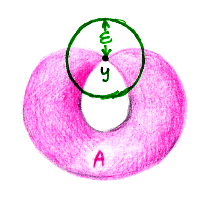
\includegraphics[height=4cm]{bearbeitet-22-04-25/loc0dc.png}
        \caption{Beispiel für eine lokal $0$-dimensional zusammenhängende Raumregion}
        \label{fig:loc0dc}
    \end{figure}
    
    In ähnlicher Weise wird dieser Begriff für Flächenregionen und für lokal $1$-dimensional zusammenhängende Raumregionen definiert.

    \begin{dfn}[Lokal 0/1-zusammenhängend in der \strukt]\ \vspace{0pt}

        \begin{itemize}
            \item Eine Raumregion $A$ ist lokal $0$-dimensional zusammenhängend im Punkt $[A', B', C', \{y\}]$, wenn gilt
            \begin{align*}
                &\Stangpart([A', B', C', \{y\}],A) \land \exists \varepsilon \forall \eta: (\eta < \varepsilon \to 
                \\
                &\SzeroDC(\ball_{\eta}(y) \cap A) \land \neg \SoneDC(\ball_{\eta}(y) \cap A))
            \end{align*}
            \item Eine Flächeregion $[A,B]$ ist lokal $0$-dimensional zusammenhängend im Punkt $[A', B', C', \{y\}]$, wenn gilt
            \begin{align*}
                &\Stangpart([A', B', C', \{y\}],[A,B]) \land \exists \varepsilon \forall \eta:
                %\\
                (\eta < \varepsilon \to
                \\
                &\SzeroDC([A,\ball_{\eta}(y) \cap B]) \land \neg \SoneDC([A,\ball_{\eta}(y) \cap B]))
            \end{align*}
            \item Eine Raumregion $A$ ist lokal $1$-dimensional zusammenhängend im Punkt $[A', B', C', \{y\}]$, wenn gilt
            \begin{align*}
                &\Stangpart([A', B', C', \{y\}],A) \land \exists \varepsilon \forall \eta: (\eta < \varepsilon \to 
                \\
                &\SoneDC(\ball_{\eta}(y) \cap A) \land \neg \StwoDC(\ball_{\eta}(y) \cap A))
            \end{align*}
        \end{itemize}
        
    \end{dfn}
%     
%     In Abbildung \ref{fig:lok0dc} ist ein Beispiel einer lokal 0-dimensional zusammenhängenden Raumregion dargestellt.
%     


    Da es in $\theoryBS$ keinen Abstandsbegriff gibt, lässt sich diese Definition nicht so ohne weiteres auf die Theorie hochziehen. 
    In $\theoryBS$ definiere ich den lokalen Zusammenhang auf folgende Weise:

    % Wenn wir erst den Begriff des maximaldimensionalen zusammenhangs einführen, müssen wir dafür nicht zwischen Raum- und Flächenregionen unterscheiden.
    % 
    % Eine Raumentität ist maximaldimensional zusammenhängend, wenn sie aufgrund ihrer Dimension nicht stärker zusammenhängend sein kann.
    % 
    % \begin{dfn}[$x$ ist maximaldimensional zusammenhängend]
    %     \begin{align*}
    %         \Gmaxcon(x) := 
    %             &(\GSReg(x) \wedge \GtwoDC(x)) \lor 
    %             (\GtwoDE(x) \land \GoneDC(x)) \lor
    %             \\
    %             &(\GoneDE(x) \land \GzeroDC(x)) \lor \GzeroD(x)
    %     \end{align*}
    % 
    % \end{dfn}


    \begin{dfn}[$x$ ist lokal $0$/$1$-dimensional zusammenhängend in $y$]
        \begin{align*}
            \Gloczerodc(x,y) := &\GzeroD(y) \land \Gtangpart(y,x) \land
                                \\
                                &\exists u\ (\forall v w\ (\Ginpart(y,v) \land \Gspart(v,u) \land
                                \\
                                &\Gintersect(x,v,w) \to \neg \GoneDC(w)))
                                \\
            \Gloconedc(x,y) := &\neg \Gloczerodc(x,y) \land \GzeroD(y) \land \Gtangpart(y,x) \land
                                \\
                                &\exists u\ (\forall v w\ (\Ginpart(y,v) \land \Gspart(v,u) \land
                                \\
                                &\Gintersect(x,v,w) \to \neg \GtwoDC(w)))
        \end{align*}

    \end{dfn}

    Es ist noch zu zeigen, dass beide Definitionen kompatibel sind.
    Abbildung \ref{fig:loc1dc} zeigt ein Beispiel einer lokal $1$-dimensional zusammenhängenden Raumregion.

    \begin{figure}[ht]
            \centering
            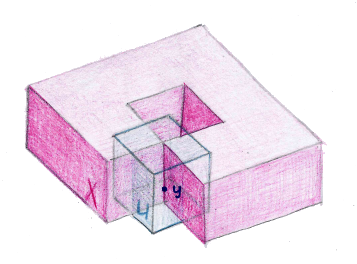
\includegraphics[width=0.6\textwidth]{bearbeitet-22-04-25/loc1dc.png}
            \caption[Beispiel für eine lokal $1$-dimensional zusammenhängende Raumregion]{Beispiel für eine lokal $1$-dimensional zusammenhängende Raumregion: $x$ ist lokal $1$-dimensional zusammenhängend in $y$, da es eine Umgebung $u$ von $y$ gibt, der keinen Teil hat, der auch eine Umgebung von $y$ ist und dessen Schnitt mit $x$ $2$-dimensional zusammen hängt.}
            \label{fig:loc1dc}
    \end{figure}


% \small

% \changetext{}{2cm}{-2cm}{}{} % Anpassung der Seitenränder

% Beweise topologische Grundlagen
\chapter{Beweise}
\section{Zu Kapitel \ref{chap:topologie-grundlagen} (Grundlagen der Topologie)}

\subsection{Zu Abschnitt \ref{sec:allg-top-raeume} (Allgemeine topologische Räume)}

% --- satz:cl --------------------------------------------------------------------

\subsubsection{zu Satz \ref{satz:cl}.\ref{satz:cl.1}}\label{anh:cl.1}
    Zu zeigen ist: 
    \begin{enumerate}
        \item Aus $\mathcal{M}_A^C := \{ U \in \offen \mid U \cap A = \varnothing\}$ und $U_A^C := \bigcup\limits_{U \in \mathcal{M}_A^C} U$ folgt $\cl(A) = X \setminus U_A^C$. \label{anh:cl.1.1}
        \item $A \subseteq \cl(A)$ \label{anh:cl.1.2}
        \item Es gibt keine kleinere in $X$ abgeschlossene Obermenge von $A$ als $\cl(A)$ \label{anh:cl.1.3}
    \end{enumerate}

    \noindent	
    \textbf{Zu \ref{anh:cl.1.1}:}
        \begin{align*}
            \cl(A) &= \{x \in X \mid \forall\: U \in \offen : (\: x \in U \deshalb U \cap A \neq \varnothing \:) \} &\\
            &= \{x \in X \mid \forall\: U \in \offen : (\: U \cap A = \varnothing \deshalb x \notin U \:) \} &\\
            &= \{x \in X \mid \forall\: U \in \mathcal{M}_A^C : x \notin U \} &\\
        %	&= \{x \in X \mid x \notin \bigcup\limits_{U \in \mathcal{M}_A^C} U \} &\\
            &= \{x \in X \mid x \notin U_A^C \} &= X \setminus U_A^C
        \end{align*}

    \noindent	
    \textbf{Zu \ref{anh:cl.1.2}:} 
        Sei $x \in A$. Dann gilt $\forall\: U \in \offen : (\: x \in U \deshalb U \cap A \neq \varnothing \:)$ und somit $x \in \cl(A)$

    \noindent
    \textbf{Zu \ref{anh:cl.1.3}:}
        Sei $V \in \abg$ mit $A \subseteq V$. Sei $W := X \setminus V$. Dann gelten $W \in \offen$ und $W \cap A = \varnothing$. Damit ist $W \in \mathcal{M}_A^C$ und somit $W \subseteq U_A^C$. Also gilt $ V = X \setminus W \supseteq X \setminus U_A^C = \cl(A)$
        

\subsubsection{Zu Satz \ref{satz:cl}.\ref{satz:cl.2}} \label{anh:cl.2}
    Zu Zeigen ist: $\cl(A) = A \cup \rand(A)$.\\

    \noindent
    \textbf{\glqq$\boldsymbol{\subseteq}$\grqq:}

        \begin{longtable}{r c c l}
            & & 1. & Sei $x \in \cl(A)$ \\
            & & 2. & Angen. $x \notin A \cup \rand(A)$ \\
            2 & $\deshalb$ & 3. & $x \notin \rand(A)$ \\
            3 & $\deshalb$ & 4. & $\exists\: U \in \offen : (\: x \in U \:\land\: (\: U \cap A = \varnothing \:\lor\: U \setminus A = \varnothing \:))$ \\
            4 & $\deshalb$ & 5. & Sei $U \in \offen$ mit $x \in U$ und $U \cap A = \varnothing \:\lor\: U \setminus A = \varnothing$ \\
            2 & $\deshalb$ & 6. & $x \notin A$ \\
            5, 6 & $\deshalb$ & 7. & $x \in U \setminus A$ \\
            7 & $\deshalb$ & 9. & $U \cap A = \varnothing$ \\
            1 & $\deshalb$ & 10. & $\forall\: U \in \offen : (\: x \in U \to U \cap A \neq \varnothing \:)$ \\
            10, 5 & $\deshalb$ & 11. & $U \cap A \neq \varnothing$ \\
            9, 10 & $\deshalb$ & 12. & $\lightning$ 
        \end{longtable}	

    \noindent
    \textbf{\glqq$\boldsymbol{\supseteq}$\grqq:}

        \begin{longtable}{r c c l}
            & & 1. & Sei $x \in A \cup \rand(A)$ \\
            & & 2. & Angen. $x \notin \cl(A)$ \\
            2 & $\deshalb$ & 3. & $\exists\: U \in \offen : (\: x \in U \:\land\: U \cap A = \varnothing \:)$ \\
            3 & $\deshalb$ & 4. & Sei $U \in \offen$ mit $x \in U$ und $U \cap A = \varnothing$ \\
            4 & $\deshalb$ & 5. & $x \notin A$ \\
            1, 5 & $\deshalb$ & 6. & $x \in \rand(A)$ \\
            6 & $\deshalb$ & 7. & $\forall\: U \in \offen : (\: x \in U \to U \cap A \neq \varnothing \:\land\: U \setminus A \neq \varnothing \:)$ \\
            7, 4 & $\deshalb$ & 8. & $U \cap A \neq \varnothing$ \\
            4, 8 & $\deshalb$ & 9. & $\lightning$ 
        \end{longtable}	


\subsubsection{Zu Satz \ref{satz:cl}.\ref{satz:cl.3}} 
    Zu zeigen ist: $\cl(A \cap B) \subseteq \cl(A) \cap \cl(B)$ \\
    \begin{align*}
        &cl(A \cap B) \\
        &= \{x \in X \mid \forall\: U \in \offen : (\: x \in U \to U \cap A \cap B \neq \varnothing \:) \}\\
        &= \{x \in X \mid \forall\: U \in \offen : (\: x \in U \to (U \cap A) \cap (U \cap B) \neq \varnothing \:) \}\\
        &\subseteq \{x \in X \mid \forall\: U \in \offen : (\: x \in U \to U \cap A \neq \varnothing \:\land\: U \cap B \neq \varnothing \:) \}\\
        &= \{x \in X \mid \forall\: U \in \offen : \\
        &\hphantom{XXXXXXX} ((\: x \in U \to U \cap A \neq \varnothing \:) \:\land\: (\: x \in U \to U \cap B \neq \varnothing \:)) \}\\
        &= \{x \in X \mid \forall\: U \in \offen : (\: x \in U \to U \cap A \neq \varnothing \:) \:\land\: \\
        &\hphantom{XXXXXXX} \forall\: U \in \offen :  (\: x \in U \to U \cap B \neq \varnothing \:) \}\\
        &= \{x \in X \mid \forall\: U \in \offen : (\: x \in U \to U \cap A \neq \varnothing \:) \} \cap \\
        &\hphantom{XXXXXXX} \{x \in X \mid \forall\: U \in \offen :  (\: x \in U \to U \cap B \neq \varnothing \:) \}\\
        &= \cl(A) \cap \cl(B)
    \end{align*}


\subsubsection{Zu Satz \ref{satz:cl}.\ref{satz:cl.4}}
    Zu Zeigen ist: $\cl(A \cup B) = \cl(A) \cup \cl(B)$.\\

    \noindent
    \textbf{\glqq$\boldsymbol{\subseteq}$\grqq:}\\
        Da ${\cl(A),\cl(B) \in \abg}$ sind, ist auch ${\cl(A) \cup \cl(B) \in \abg}$ (Satz \ref{satz:CX}) und somit ${\cl(\cl(A) \cup \cl(B))= \cl(A) \cup \cl(B)}$ (Korollar \ref{kor:cl}.\ref{kor:cl.3}). Wegen ${A \subseteq \cl(A)}$ und ${B \subseteq \cl(B)}$ (ebenfalls Satz \ref{satz:CX}) gilt dann
        \begin{align*}
            \cl(A \cup B) \subseteq \cl(\cl(A) \cup \cl(B)) = \cl(A) \cup \cl(B).
        \end{align*}

    \noindent
    \textbf{\glqq$\boldsymbol{\supseteq}$\grqq:}

        \begin{longtable}{r c c l}
            & & 1. & Sei $x \in \cl(A) \cup \cl(B)$ \\
            & & 2. & Angen. $x \notin \cl(A \cup B)$ \\
            2 & $\deshalb$ & 3. & $\exists\: U \in \offen : (\: x \in U \:\land\: U \cap (A \cup B) = \varnothing \:)$ \\
            3 & $\deshalb$ & 4. & Sei $U \in \offen$ mit $x \in U$ und $U \cap (A \cup B) = \varnothing$ \\
            4 & $\deshalb$ & 5. & $(U \cap A) \cup (A \cap B) = \varnothing$ \\
            1 & $\deshalb$ & 6. & $x \in \cl(A) \:\lor\: x \in \cl(B)$ \\
            6 & $\deshalb$ & 7. & $\forall\: U \in \offen : (\: x \in U \to U \cap A \neq \varnothing \:) \:\lor\: \forall\: U \in \offen : (\: x \in U \to U \cap B \neq \varnothing \:)$ \\
            7 & $\deshalb$ & 8. & $\forall\: U \in \offen : ((\: x \in U \to U \cap A \neq \varnothing \:) \:\lor\: (\: x \in U \to U \cap B \neq \varnothing \:))$ \\
            8 & $\deshalb$ & 9. & $\forall\: U \in \offen : (\: x \in U \to (\: U \cap A \neq \varnothing \:\lor\: U \cap B \neq \varnothing \:))$ \\
            9, 4 & $\deshalb$ & 10. & $U \cap A \neq \varnothing \:\lor\: U \cap B \neq \varnothing$ \\
            10 & $\deshalb$ & 11. & $(U \cap A) \cup (U \cap B) \neq \varnothing$ \\
            5, 11 & $\deshalb$ & 12. & $\lightning$ 
        \end{longtable}	
        
        
\subsubsection{Zu Satz \ref{satz:cl}.\ref{satz:cl.5}} 
    Zu zeigen ist: $\cl(X \setminus A) = X \setminus \op(A)$ \\
    \begin{align*}
        \cl(X \setminus A)
        &= \{x \in X \mid \forall\: U \in \offen(x) : U \setminus A \neq \varnothing \}\\
        &= \{x \in X \mid \forall\: U \in \offen(x) : U \nsubseteq A \}\\
        &= \{x \in X \mid \neg \exists\: U \in \offen(x) : U \subseteq A \}\\
        &= X \setminus \op(A)
    \end{align*}


\subsubsection{Zu Satz \ref{satz:cl}.\ref{satz:cl.6}}
    Zu Zeigen ist: $\cl(A \setminus B) \subseteq \cl(A) \setminus \op(B)$.\\

    \begin{longtable}{r c c l}
        & & 1. & Sei $x \in \cl(A \setminus B)$ \\
        1. & $\deshalb$ & 2. & $\forall\: U \in \offen : (\: x \in U \to U \cap (A \setminus B) \neq \varnothing \:)$ \\
        2 & $\deshalb$ & 3. & $\forall\: U \in \offen : (\: x \in U \to (U \cap A) \cap (U \setminus B) \neq \varnothing \:)$ \\
        3 & $\deshalb$ & 4. & $\forall\: U \in \offen : (\: x \in U \to (U \cap A) \neq \varnothing \:\land\: (U \setminus B) \neq \varnothing \:)$ \\
        4 & $\deshalb$ & 5. & $\forall\: U \in \offen : ( (\: x \in U \to U \cap A \neq \varnothing \:) \:\land\: (\: x \in U \to U \setminus B \neq \varnothing \:))$ \\
        5 & $\deshalb$ & 6. & $\forall\: U \in \offen : (\: x \in U \to U \cap A \neq \varnothing \:) \:\land\: \forall\: U \in \offen : (\: x \in U \to U \setminus B \neq \varnothing \:)$ \\
        6 & $\deshalb$ & 7. & $x \in \cl(A)$ und $\neg \exists\: U \in \offen : (\: x \in U \:\land\: U \setminus B = \varnothing \:)$ \\
        7 & $\deshalb$ & 8. & $x \in \cl(A)$ und $\neg \exists\: U \in \offen : (\: x \in U \:\land\: U \subseteq B \:)$ \\
        8 & $\deshalb$ & 9. & $x \in \cl(A)$ und $x \notin \op(B)$ \\
        9 & $\deshalb$ & 10. & $x \in \cl(A) \setminus \op(B)$ \\
    \end{longtable}


\subsubsection{Zu Satz \ref{satz:cl}.\ref{satz:cl.7}} 
    Zu zeigen ist: $\cl(A) \setminus \cl(B) \subseteq \cl(A \setminus B)$

    \begin{longtable}{r c c l}
        & & 1. & Sei $x \in \cl(A) \setminus \cl(B)$ \\
        & & 2. & Angen. $x \notin \cl(A \setminus B)$ \\
        2 & $\deshalb$ & 3. & $\exists\: U \in \offen : (\: x \in U \:\land\: U \cap (A \setminus B) = \varnothing \:)$ \\
        3 & $\deshalb$ & 4. & Sei $U_0 \in \offen$ mit $x \in U_0$ und $U_0 \cap (A \setminus B) = \varnothing$ \\
        1 & $\deshalb$ & 5. & $x \notin \cl(B)$ \\
        5 & $\deshalb$ & 6. & $\exists\: U \in \offen : (\: x \in U \:\land\: U \cap B = \varnothing \:)$ \\
        6 & $\deshalb$ & 7. & Sei $U_1 \in \offen$ mit $x \in U_1$ und $U_1 \cap B = \varnothing$ \\
        1 & $\deshalb$ & 8. & $\forall\: U \in \offen : (\: x \in U \to U \cap A \neq \varnothing \:)$ \\
        4, 7 & $\deshalb$ & 9. & Sei $U_2 := U_0 \cap U_1$ \\
        9, 4, 7 & $\deshalb$ & 10. & $x \in U_2 \in \offen$ \\
        10, 8 & $\deshalb$ & 11. & $U_2 \cap A \neq \varnothing$ \\
        11 & $\deshalb$ & 12. & Sei $y \in U_2 \cap A$ \\
        12 & $\deshalb$ & 13. & $y \in U_2$ \\
        13, 9 & $\deshalb$ & 14. & $y \in U_1$ \\
        14, 7 & $\deshalb$ & 15. & $y \notin B$ \\
        12 & $\deshalb$ & 16. & $y \in A$ \\
        16, 15 & $\deshalb$ & 17. & $y \in A \setminus B$ \\
        13, 9 & $\deshalb$ & 18. & $y \in U_0$ \\
        18, 17 & $\deshalb$ & 19. & $y \in U_0 \cap (A \setminus B)$ \\
        19, 4 & $\deshalb$ & 20. & $\lightning$
    \end{longtable}


\subsubsection{Zu Satz \ref{satz:cl}.\ref{satz:cl.8}} \label{anh:cl.8}
    Zu zeigen: Aus ${A \subseteq B}$ folgt ${\cl(A) \subseteq \cl(B)}$.\\
    Gelte ${A \subseteq B}$ und sei ${x \notin \cl(B)}$. Dann gibt es ein ${U \in \offen}$ mit ${x \in U}$ und ${U \cap B = \varnothing}$. Da für so ein $U$ gilt ${U \cap A \subseteq U \cap B}$, ist dann natürlich auch ${U \cap A = \varnothing}$. Somit gilt: ${\exists\: U \in \offen : (\: x \in U \:\land\: U \cap A = \varnothing \:)}$. Also ist ${x \notin \cl(A)}$.

    
% --- satz:op -----------------------------------------------------------------

\subsubsection{Zu Satz \ref{satz:op}.\ref{satz:op.2}}\label{anh:op.2}
    Zu zeigen ist: $\op(A) = A \setminus \rand(A)$.\\

    \noindent
    \textbf{\glqq$\boldsymbol{\subseteq}$\grqq:}

        \begin{longtable}{r c c l}
            & & 1. & Sei $x \in \op(A)$ \\
            & & 2. & Angen. $x \notin A \setminus \rand(A)$ \\
            1 & $\deshalb$ & 3. & $\exists\: U \in \offen : (\: x \in U \:\land\: U \subseteq A \:)$ \\
            3 & $\deshalb$ & 4. & Sei $U \in \offen$ mit $x \in U$ und $U \subseteq A$. \\
            4 & $\deshalb$ & 5. & $x \in A$ \\
            2, 5 & $\deshalb$ & 6. & $x \in \rand(A)$ \\
            6 & $\deshalb$ & 7. & $\forall\: U \in \offen : (\: x \in U \to U \cap A \neq \varnothing \:\land\: U \setminus A \neq \varnothing \:)$ \\
            7, 4 & $\deshalb$ & 8. & $U \setminus A \neq \varnothing$ \\
            4, 8 & $\deshalb$ & 9. & $\lightning$ 
        \end{longtable}	

    \noindent
    \textbf{\glqq$\boldsymbol{\supseteq}$\grqq:}

        \begin{longtable}{r c c l}
            & & 1. & Sei $x \in A \setminus \rand(A)$ \\
            & & 2. & Angen. $x \notin \op(A)$ \\
            1 & $\deshalb$ & 3. & $x \notin \rand(A)$ \\
            3 & $\deshalb$ & 4. & $\exists\: U \in \offen : (\: x \in U \:\land\: (\: U \cap A = \varnothing \:\lor\: U \setminus A = \varnothing \:))$ \\
            4 & $\deshalb$ & 5. & Sei $U \in \offen$ mit $x \in U$ und $U \cap A = \varnothing \:\lor\: U \setminus A = \varnothing$ \\
            2 & $\deshalb$ & 6. & $\forall\: U \in \offen : (\: x \in U \to U \setminus A \neq \varnothing \:)$ \\
            5, 6 & $\deshalb$ & 7. & $U \setminus A \neq \varnothing$ \\
            7, 4 & $\deshalb$ & 8. & $U \cap A = \varnothing$ \\
            1 & $\deshalb$ & 9. & $x \in A$ \\
            5, 9 & $\deshalb$ & 10. & $x \in U \cap A$ \\	
            8, 10 & $\deshalb$ & 12. & $\lightning$ 
        \end{longtable}


\subsubsection{Zum Beweis von Satz \ref{satz:op}.\ref{satz:op.1}}\label{anh:op.1}
    Zu zeigen ist: Aus ${\mathcal{M}_A := \{U \in \offen \mid U \subseteq A\}}$ folgt $\op(A) = \bigcup\limits_{U \in \mathcal{M}_A} U$.\\

    \noindent
    \textbf{"$\boldsymbol{\subseteq}$":} 
    Sei $x \in \op(A)$. Dann gibt es ein ${U \in \offen}$ mit $x \in U$ und ${U \subseteq A}$. Also ist ${U \in \mathcal{M}_A}$ und somit ${x \in U \subseteq \bigcup\limits_{U \in \mathcal{M}_A} U}$.

    \noindent
    \textbf{"$\boldsymbol{\supseteq}$":}
    Sei $x \in \bigcup\limits_{U \in \mathcal{M}_A} U$. Sei $U \in \mathcal{M}_A$ mit $x \in U$. Dann gelten: $U \in \offen$ und $U \subseteq A$. Also ist $x \in \op(A)$.


\subsubsection{Zu Satz \ref{satz:op}.\ref{satz:op.3}}\label{anh:op.3}
    Zu zeigen ist: $\op(A \cap B) = \op(A) \cap \op(B)$.\\

    \noindent
    \textbf{"$\boldsymbol{\subseteq}$":}
        \begin{align*}
            \op(A \cap B) 
            &= \{x \in X \mid \exists\: U \in \offen: (\: x \in U \:\land\: U \subseteq A \cap B \:)\}\\
            &= \{x \in X \mid \exists\: U \in \offen: (\: x \in U \:\land\: U \subseteq A \:\land\: U \subseteq B \:)\}\\
            &\subseteq \{x \in X \mid \exists\: U \in \offen: (\: x \in U \:\land\: U \subseteq A\:) \:\land\: \\
            &\hphantom{XXXXXXX} \exists\: U \in \offen: (\: x \in U \:\land\: U \subseteq B \:)\}\\
            &= \{x \in X \mid \exists\: U \in \offen: (\: x \in U \:\land\: U \subseteq A\:)\} \cap\\
            &\hphantom{XXXXXXX} \{ x \in X \mid \exists\: U \in \offen: (\: x \in U \:\land\: U \subseteq B \:)\}\\
            &= \op(A) \cap \op(B)
        \end{align*}

    \noindent
    \textbf{"$\boldsymbol{\supseteq}$":}
        \begin{longtable}{r c c l}
            & & 1. & Sei $x \in \op(A) \cap \op(B)$ \\
            1 & $\deshalb$ & 2. & $x \in \op(A)$ \\
            2 & $\deshalb$ & 3. & $\exists\: U \in \offen: (\: x \in U \:\land\: U \subseteq A\:)$ \\
            3 & $\deshalb$ & 4. & Sei $U_A \in \offen$ mit $x \in U_A$ und $U_A \subseteq A$ \\
            1 & $\deshalb$ & 5. & $x \in \op(B)$ \\
            5 & $\deshalb$ & 6. & $\exists\: U \in \offen: (\: x \in U \:\land\: U \subseteq B\:)$ \\
            6 & $\deshalb$ & 7. & Sei $U_B \in \offen$ mit $x \in U_B$ und $U_B \subseteq B$ \\
            4, 7 & $\deshalb$ & 8. & Sei $U := U_A \cap U_B$ \\
            4, 7, 8 & $\deshalb$ & 9. & $x \in U$ \\
            4, 7, 8 & $\deshalb$ & 10. & $U \subseteq A \cap B$ \\
            9, 10 & $\deshalb$ & 11. & $x \in \op(A \cap B)$ \\
        \end{longtable}


\subsubsection{Zu Satz \ref{satz:op}.\ref{satz:op.4}}\label{anh:op.4}
    Zu zeigen ist: $\op(A) \cup \op(B) \subseteq \op(A \cup B)$
    \begin{align*}
        &\op(A) \cup \op(B) \\
        &= \{x \in X \mid x \in \op(A) \:\lor\: x \in \op(B)\} \\
        &= \{x \in X \mid \exists\: U \in \offen : (\: x \in U \:\land\: U \subseteq A \:) \:\lor\:\\
        &\hphantom{XXXXXXX} \exists\: U \in \offen : (\: x \in U \:\land\: U \subseteq B \:) \} \\
        &= \{x \in X \mid \exists\: U \in \offen : ((\: x \in U \:\land\: U \subseteq A \:) \:\lor\: (\: x \in U \:\land\: U \subseteq B \:)) \} \\
        &= \{x \in X \mid \exists\: U \in \offen : (\: x \in U \:\land\: (\: U \subseteq A \:\lor\: U \subseteq B \:)) \} \\
        &\subseteq \{x \in X \mid \exists\: U \in \offen : (\: x \in U \:\land\: U \subseteq A \cup B \:) \} \\
        &= \op(A \cup B)
    \end{align*}
    
    
\subsubsection{Zu Satz \ref{satz:op}.\ref{satz:op.5}} 
    Zu zeigen ist: $\op(X \setminus A) = X \setminus \cl(A)$ \\
    \begin{align*}
        \op(X \setminus A)
        &= \{x \in X \mid \exists\: U \in \offen(x) : U \subseteq X \setminus A \}\\
        &= \{x \in X \mid \exists\: U \in \offen(x) : U \cap A = \varnothing\}\\
        &= \{x \in X \mid \neg \forall\: U \in \offen(x) : U \cap A \neq \varnothing \}\\
        &= X \setminus \cl(A)
    \end{align*}


\subsubsection{Zu Satz \ref{satz:op}.\ref{satz:op.6}}\label{anh:op.5}	
    Zu zeigen ist: $\op(A \setminus B) = \op(A) \setminus \cl(B)$\\

    \noindent
    \textbf{"$\boldsymbol{\subseteq}$":}
        \begin{longtable}{r r c r l}
            & & & 1. & Sei $x \in \op(A \setminus B) $ \\
            & & & 2. & Angen. $x \notin \op(A) \setminus \cl(B)$ \\
            & 1 & $\deshalb$ & 3. & $\exists\: U \in \offen : (\: x \in U \:\land\: U \subseteq A \setminus B \:)$ \\
            & 3 & $\deshalb$ & 4. & Sei $U \in \offen$ mit $x \in U$ und $U \subseteq A \setminus B$ \\
            & 4 & $\deshalb$ & 5. & $\varnothing = U \setminus (A \setminus B) = (U \setminus A) \cup (U \cap B)$ \\
            & 5 & $\deshalb$ & 6. & $U \setminus A = \varnothing$ \\
            & 6 & $\deshalb$ & 7. & $U \cap B = \varnothing$ \\
            & 2 & $\deshalb$ & 8. & $x \notin \op(A) \:\lor\: x \in \cl(B)$ \\
            \hline
            Fall 1: & 8 & $\deshalb$ & 1.9. & $x \notin \op(A)$ \\
            & 1.9. & $\deshalb$ & 1.10. & $\neg \exists\: U \in \offen : (\: x \in U \:\land\: U \subseteq A \:)$ \\
            & 1.10 & $\deshalb$ & 1.11. & $\forall\: U \in \offen : (\: x \in U \to U \setminus A \neq \varnothing \:)$ \\
            & 1.11, 4 & $\deshalb$ & 1.12. & $U \setminus A \neq \varnothing$ \\
            & 1.12, 6 & $\deshalb$ & 1.13. & $\lightning$ \\
            \hline
            Fall 2: 
            & 8 & $\deshalb$ & 2.9. & $x \in \cl(B)$ \\
            & 2.9 & $\deshalb$ & 2.10 & $\forall\: U \in \offen : (\: x \in U \to U \cap B \neq \varnothing \:)$ \\
            & 2.10, 4 & $\deshalb$ & 2.11 & $U \cap B \neq \varnothing$ \\
            & 2.11, 7 & $\deshalb$ & 2.12 & $\lightning$ \\
        \end{longtable}

    \noindent
    \textbf{"$\boldsymbol{\supseteq}$":}

        \begin{longtable}{r c c l}
            & & 1. & Sei $x \in \op(A) \setminus \cl(B)$ \\
            & & 2. & Angen. $x \notin \op(A \setminus B))$ \\
            1 & $\deshalb$ & 3. & $x \in \op(A)$ \\
            3 & $\deshalb$ & 4. & $\exists\: U \in \offen : (\: x \in U \:\land\: U \subseteq A \:)$ \\
            4 & $\deshalb$ & 5. & Sei $U_1 \in \offen$ mit $x \in U_1$ und $U_1 \subseteq A$ \\
            1 & $\deshalb$ & 6. & $x \notin \cl(B)$ \\
            6 & $\deshalb$ & 7. & $\exists\: U \in \offen : (\: x \in U \:\land\: U \cap B = \varnothing \:)$ \\
            7 & $\deshalb$ & 8. & Sei $U_2 \in \offen$ mit $x \in U_2$ und $U_2 \cap B = \varnothing$ \\
            8, 5 & $\deshalb$ & 9. & Sei $U_0 := U_1 \cap U_2 \in \offen$ \\
            9, 5, 8 & $\deshalb$ & 10. & $x \in U_0$ \\
            2 & $\deshalb$ & 11. & $\forall\: U \in \offen : (\: U \setminus (A \setminus B) \neq \varnothing \:)$ \\
            11, 9, 10 & $\deshalb$ & 12. & $U_0 \setminus (A \setminus B) \neq \varnothing$ \\
            12 & $\deshalb$ & 13. & Sei $y \in U_0 \setminus (A \setminus B)$ \\
            13 & $\deshalb$ & 14. & $y \in U_0$ \\
            14, 9 & $\deshalb$ & 15. & $y \in U_1$ \\
            15, 5 & $\deshalb$ & 16. & $y \in A$ \\
            14, 9 & $\deshalb$ & 17. & $y \in U_2$ \\
            17, 7 & $\deshalb$ & 18. & $y \notin B$ \\
            16, 18 & $\deshalb$ & 19. & $y \in A \setminus B$ \\
            19, 13 & $\deshalb$ & 20. & $\lightning$ \\
        \end{longtable}
        

% --- satz:rand ---------------------------------------------------------------------

\subsubsection{Zu Satz \ref{satz:rand}.\ref{satz:rand.1}} \label{anh:rand.1}
    Zu zeigen ist: $\rand(\rand(A)) \subseteq \rand(A))$ \\
    Sei $x \in \rand(\rand(A))$. Dann gilt nach Definition des Randoperators (Def \ref{def:rand})
    \begin{align} \label{anh:rand.1.1}
        \forall\: U \in \offen: (\: x \in U \to (\: U \cap \rand(A) \neq \varnothing \:\land\: U \setminus \rand(A) \neq \varnothing \:))
    \end{align}
    Angenommen $x \notin \rand(A)$. %Dann gilt wiederum nach der Definition des Randoperators 	
    \begin{align*} %\label{anh:rand.1.2}
        \exists\: U \in \offen : (\: x \in U \:\land\: (\: U \cap A = \varnothing \:\lor\: U \setminus A = \varnothing \:))
    \end{align*}
    Sei also $U_0 \in \offen$ mit $x \in U_0$ und
    \begin{align} \label{anh:rand.1.3}
        U_0 \cap A = \varnothing \:\lor\: U_0 \setminus A = \varnothing
    \end{align}
    nach (\ref{anh:rand.1.1}) gilt jetzt $U_0 \cap \rand(A) \neq \varnothing$. Sei also $y \in U_0 \cap \rand(A)$.
    %Dann gilt wieder nach Definition des Randoperators
    \begin{align*} %\label{anh:rand.1.4}
        \forall\: U \in \offen: (\: y \in U \to (\: U \cap A \neq \varnothing \:\land\: U \setminus A \neq \varnothing))
    \end{align*}
    Also
    \begin{align*}
        U_0 \cap A \neq \varnothing \:\land\: U_0 \setminus A \neq \varnothing
    \end{align*}
    was (\ref{anh:rand.1.3}) widerspricht.

	
\subsubsection{Zu Satz \ref{satz:rand}.\ref{satz:rand.2}}\label{anh:rand.2}
    Zu zeigen ist: $\rand(A) = \cl(A) \setminus \op(A)$
    \begin{align*}
    \cl(A) \setminus \op(A) &= &&\cl(A) \cap (X \setminus \op(A))\\
                            &= &&\{x \in X \mid \forall\: U \in \offen: (\: x \in U \to U \cap A \neq \varnothing \:)\}\\ 
                            &  &&\cap \{x \in X \mid \neg \exists\: U \in \offen: (\: x \in U \:\land\: U \subseteq A\:)\}\\
                            &= &&\{x \in X \mid \forall\: U \in \offen: (\: x \in U \to U \cap A \neq \varnothing\:) \:\land\:\\ 
                            &  &&\forall\: U \in \offen:(\: x \in U \to \neg(U \subseteq A) \:) \}\\
                            &= &&\{x \in X \mid \forall\: U \in \offen: (\: (\: x \in U \to U \cap A \neq \varnothing \:) \:\land\:\\
                            &  &&(\: x \in U \to U \setminus A \neq \varnothing \:) \:) \}\\
                            &= &&\{x \in X \mid \forall\: U \in \offen: (\: x \in U \to (\: U \cap A \neq \varnothing \:\land\: U \setminus A \neq \varnothing \:) \:) \}\\
                            &= &&\rand(A)
    \end{align*}


\subsubsection{Zu Satz \ref{satz:rand}.\ref{satz:rand.3}}\label{anh:rand.3}
    Zu zeigen ist: $(\rand(A) \cap \op(B)) \cup (\rand(B) \cap \op(A)) \subseteq \rand(A \cap B)$.\\ \ \\
    Ich zeige:
    \begin{enumerate}
    \item\label{anh:rand.3.1} $\rand(A) \cap \op(B) \subseteq \rand(A \cap B) \quad$ und
    \item\label{anh:rand.3.2} $\rand(B) \cap \op(A) \subseteq \rand(A \cap B)$
    \end{enumerate}

    \noindent
    \textbf{Zu \ref{anh:rand.3.1}: }
        \begin{longtable}{r c r l}
                    &          &  1. & Sei $x \in \rand(A) \cap \op(B)$ \\
                    &          &  2. & Angen. $x \notin \rand(A \cap B)$ \\
            1          & $\deshalb$ &  3. & $x \in \op(B)$ \\
            3          & $\deshalb$ &  4. & $\exists\: U \in \offen: (\: x \in U \:\land\: U \subseteq B \:) $ \\
            4          & $\deshalb$ &  5. & Sei $U_1 \in \offen$ mit $x \in U_1$ und $U_1 \subseteq B$ \\
            2          & $\deshalb$ &  6. & $\exists\: U \in \offen: (\: x \in U \:\land\: (\: U \cap A \cap B = \varnothing \:\lor\: U \setminus (A \cap B) = \varnothing \:) \:)$ \\
            6          & $\deshalb$ &  7. & Sei $U_2 \in \offen$ mit $x \in U_2$ und $U_2 \cap A \cap B = \varnothing \:\lor\: U_2 \setminus (A \cap B) = \varnothing$ \\
            5, 7       & $\deshalb$ &  8. & Sei $U := U_1 \cap U_2$ \\
            5, 7, 8    & $\deshalb$ &  9. & $x \in U \in \offen$ \\
            1          & $\deshalb$ & 10. & $x \in \rand(A)$ \\
            10         & $\deshalb$ & 11. & $\forall\: U \in \offen: (\: x \in U \to (\: U \cap A \neq \varnothing \:\land\: U \setminus A \neq \varnothing \:) \:) $ \\
            9, 11      & $\deshalb$ & 12. & $U \cap A \neq \varnothing \:\land\: U \setminus A \neq \varnothing$ \\
            12         & $\deshalb$ & 13. & Sei $y \in U \setminus A$ \\
            13, 8      & $\deshalb$ & 14. & $y \in U_2$ \\
            13         & $\deshalb$ & 15. & $y \notin A \supseteq A \cap B$ \\
            14, 15     & $\deshalb$ & 16. & $y \in U_2 \setminus (A \cap B)$ \\
            7, 16      & $\deshalb$ & 17. & $U_2 \cap A \cap B = \varnothing$ \\
            11         & $\deshalb$ & 18. & Sei $z \in U \cap A$ \\
            8, 18      & $\deshalb$ & 19. & $z \in U_1$ \\
            5, 19      & $\deshalb$ & 20. & $z \in B$ \\
            8, 18      & $\deshalb$ & 21. & $z \in U_2$ \\
            18, 20, 21 & $\deshalb$ & 22. & $z \in U_2 \cap A \cap B$ \\
            17, 22     & $\deshalb$ & 23. & $\lightning$
        \end{longtable}

    \noindent
    \textbf{Zu \ref{anh:rand.3.1}: } analog

\subsubsection{Zu Satz \ref{satz:rand}.\ref{satz:rand.4}}\label{anh:rand.4}
    Zu zeigen ist: $\rand(A \cap B) \subseteq (\rand(A) \cap \cl(B)) \cup (\rand(B) \cap \cl(A))$.\\ \ \\

    \noindent
    \textbf{Vorüberlegung (*): } Für beliebige $A, B \subseteq X$ gilt:
        \begin{align*}
            &\rand(A) \cap \cl(B) \\ 
            &= \{x \in X \mid \forall\: U \in \offen: (\: x \in U \to (\: U \cap A \neq \varnothing \:\land\: U \setminus A \neq \varnothing \:) \:)\}\\
            &\hphantom{XXXXXXX}\cap \{x \in X \mid \forall\: U \in \offen: (\: x \in U \to U \cap B \neq \varnothing \:)\}\\
            &= \{x \in X \mid \forall\: U \in \offen: (\: x \in U \to (\: U \cap A \neq \varnothing \:\land\:\\
            &\hphantom{XXXXXXX} U \setminus A \neq \varnothing \:\land\: U \cap B \neq \varnothing \:) \:)\}
        \end{align*}

    \begin{longtable}{r c r l}
        & & 1. & Sei $x \in \rand(A \cap B)$ \\
        & & 2. & Angen. $x \notin (\rand(A) \cap \cl(B)) \cup (\rand(B) \cap \cl(A))$ \\
        2 & $\deshalb$ & 3. & $x \notin \rand(A) \cap \cl(B)$ \\
        3, * & $\deshalb$ & 4. & $\exists\: U \in \offen: (\: x \in U \:\land\:$\\
                             &&& $(\: U \cap A = \varnothing \:\lor\: U \setminus A = \varnothing \:\lor\: U \cap B = \varnothing \:) \:) $ \\
        4 & $\deshalb$ & 5. & Sei $U_1 \in \offen$ mit $x \in U_1$ und\\
                              &&& $U_1 \cap A = \varnothing \:\lor\: U_1 \setminus A = \varnothing \:\lor\: U_1 \cap B = \varnothing$ \\
        2 & $\deshalb$ & 6. & $x \notin \rand(B) \cap \cl(A)$ \\
        6, * & $\deshalb$ & 7. & $\exists\: U \in \offen: (\: x \in U \:\land\:$\\
                             &&& $(\: U \cap B = \varnothing \:\lor\: U \setminus B = \varnothing \:\lor\: U \cap A = \varnothing \:) \:)$ \\
        7 & $\deshalb$ & 8. & Sei $U_2 \in \offen$ mit $x \in U_2$ und\\
                          &&& $U_2 \cap B = \varnothing \:\lor\: U_2 \setminus B = \varnothing \:\lor\: U_2 \cap A = \varnothing$\\
        5, 8 & $\deshalb$ & 9. & Sei $U := U_1 \cap U_2$ \\
        1 & $\deshalb$ & 10. & $\forall\: U \in \offen: (\: x \in U \to$\\
                           &&& $U \cap A \cap B \neq \varnothing \:\land\: U \setminus (A \cap B) \neq \varnothing \:) \:) $ \\
        5, 8, 9 & $\deshalb$ & 11. & $x \in U \in \offen$ \\
        10, 11 & $\deshalb$ & 12. & $U \cap A \cap B \neq \varnothing$ und $U \setminus (A \cap B) \neq \varnothing$ \\
        9, 12 & $\deshalb$ & 13. & $U_1 \cap U_2 \cap A \cap B \neq \varnothing$ \\
        13 & $\deshalb$ & 14. & $U_1 \cap A \neq \varnothing$ \\
        13 & $\deshalb$ & 15. & $U_1 \cap B \neq \varnothing$ \\
        5, 14, 15 & $\deshalb$ & 16. & $U_1 \setminus A = \varnothing$ \\
        9, 16 & $\deshalb$ & 17. & $U \setminus A = (U_1 \cap U_2) \setminus A \subseteq U_1 \setminus A = \varnothing$ \\
        13 & $\deshalb$ & 18. & $U_2 \cap A \neq \varnothing$ \\
        13 & $\deshalb$ & 19. & $U_2 \cap B \neq \varnothing$ \\
        8, 18, 19 & $\deshalb$ & 20. & $U_2 \setminus B = \varnothing$ \\
        9, 20 & $\deshalb$ & 21. & $U \setminus B = (U_1 \cap U_2) \setminus B \subseteq U_2 \setminus B = \varnothing $ \\
        17, 21 & $\deshalb$ & 22. & $\varnothing = (U \setminus A) \cup (U \setminus B) = U \setminus (A \cap B) $ \\
        12, 22 & $\deshalb$ & 23. & $\lightning$
    \end{longtable}


\subsubsection{Zu Satz \ref{satz:rand}.\ref{satz:rand.7}}\label{anh:rand.7}
    Zu zeigen ist: $\rand(A \setminus B) \subseteq (\rand(A) \setminus \op(B)) \cup (\rand(B) \cap \cl(A))$

    \begin{longtable}{r r c r l}
        & & & 1. & Sei $x \in \rand(A \setminus B) $ \\
        & & & 2. & Angen. $x \notin (\rand(A) \setminus \op(B)) \cup (\rand(B) \cap \cl(A))$ \\
        & 1 & $\deshalb$ & 3. & $\forall\: U \in \offen : (\: x \in U \to$\\
                           &&&& $(\: U \cap (A \setminus B) \neq \varnothing \:\land\: U \setminus (A \setminus B) \neq \varnothing \:))$ \\
        & 2 & $\deshalb$ & 4. & $x \notin \rand(A) \setminus \op(B)$ \\
        & 4 & $\deshalb$ & 5. & $x \notin \rand(A) \:\lor\: x \in \op(B)$ \\
        \hline
        Fall 1: & & & 1.1. & $x \in \op(B)$ \\
        &  & $\deshalb$ & 1.2. & $\exists\: U \in \offen : (\: x \in U \:\land\: U \subseteq B \:)$ \\
        & 1.2 & $\deshalb$ & 1.3. & Sei $U \in \offen$ mit $x \in U$ und $U \subseteq B$  \\
        & 3, 1.3 & $\deshalb$ & 1.4. & $U \cap (A \setminus B) \neq \varnothing$ \\
        & 1.4 & $\deshalb$ & 1.5. & $U \setminus B \neq \varnothing$ \\
        & 1.5, 1.3 & $\deshalb$ & 1.6. & $\lightning$ \\
        \hline
        Fall 2: & & & 2.1. & $x \notin \op(B)$ \\
        & 5, 2.1 & $\deshalb$ & 2.2. & $x \notin \rand(A)$ \\
        & 2.2 & $\deshalb$ & 2.3. & $\exists\: U \in \offen : (\: x \in U \:\land\: (\: U \cap A = \varnothing \:\lor\: U \setminus A = \varnothing \:))$ \\
        & 2.3 & $\deshalb$ & 2.4. & Sei $U_0 \in \offen$ mit $x \in U_0$ und\\
                               &&&& $U_0 \cap A = \varnothing \:\lor\: U_0 \setminus A = \varnothing$ \\
        & 3, 2.4 & $\deshalb$ & 2.5. & $U_0 \cap (A \setminus B) \neq \varnothing$ \\
        & 2.5 & $\deshalb$ & 2.6. & $U_0 \cap A \neq \varnothing$ \\
        & 2.6, 2.4 & $\deshalb$ & 2.7. & $U_0 \setminus A = \varnothing$ \\
        & 2.4, 2.7 & $\deshalb$ & 2.8. & $x \in A$ \\
        & 2.8 & $\deshalb$ & 2.9. & $x \in \cl(A)$ \\
        & 2 & $\deshalb$ & 2.10. & $x \notin \rand(B) \cap \cl(A)$ \\
        & 2.10, 2.9 & $\deshalb$ & 2.11. & $x \notin \rand(B)$ \\
        & 2.11 & $\deshalb$ & 2.12. & $\exists\: U \in \offen : (\: x \in U \:\land\: (\: U \cap B = \varnothing \:\lor\: U \setminus B = \varnothing \:))$ \\
        & 2.12 & $\deshalb$ & 2.13. & Sei $U_1 \in \offen$ mit $x \in U_1$ und\\
                                 &&&& $U_1 \cap B = \varnothing \:\lor\: U_1 \setminus B = \varnothing$ \\
        & 2.11, 2.1 & $\deshalb$ & 2.14. & $x \notin \cl(B) \subseteq B$ \\
        & 2.13, 2.14 & $\deshalb$ & 2.15. & $x \in U_1 \setminus B$ \\
        & 2.15 & $\deshalb$ & 2.16. & $U_1 \setminus B \neq \varnothing$ \\
        & 2.16, 2.13 & $\deshalb$ & 2.17. & $U_1 \cap B = \varnothing$ \\
        & 2.13, 2.4 & $\deshalb$ & 2.18. & Sei $U_2 := U_0 \cap U_1 \in \offen$ \\
        & 2.13, 2.4, 2.18 & $\deshalb$ & 2.19. & $x \in U_2$ \\
        & 3, 2.18, 2.19 & $\deshalb$ & 2.20. & $U_2 \setminus (A \setminus B) \neq \varnothing$ \\
        & 2.18 & $\deshalb$ & 2.23. & $U_2 \subseteq U_0$ \\
        & 2.23, 2.7 & $\deshalb$ & 2.24. & $U_2 \setminus A = \varnothing$ \\
        & 2.18 & $\deshalb$ & 2.25. & $U_2 \subseteq U_1$ \\
        & 2.17, 2.25 & $\deshalb$ & 2.26. & $U_2 \cap B = \varnothing$ \\
        & 2.24, 2.26 & $\deshalb$ & 2.27. & $\varnothing = (U_2 \setminus A) \cup (U_2 \cap B)$\\
                                       &&&& $= U_2 \setminus (A \setminus B)$ \\
        & 2.17, 2.20 & $\deshalb$ & 2.28. & $\lightning$ \\
    \end{longtable}
    
    
% --- bsp:standardbsp-rand-hp -----------------------------------------------------

\subsubsection{Zu Bsp.~\ref{bsp:standardbsp-rand-hp}}\label{anh:standardbsp-rand-hp}
    Zu zeigen ist: Für $\rand A = \{\frac{1}{2^n} \mid n \in \N\} \cup \{0\}$ ist $0$ der einzige Häufungspunkt.\\ \ \\
    %
    Sei $x \in \R$.\\ \ \\
        \textbf{Fall 1:} $x < 0$.\\
            Dann ist $U := (2x,\frac{x}{2})$ eine offene Umgebung von $x$ in $\R$ mit $\varnothing = U \cap \rand A \subseteq U \cap (\rand A \setminus \{x\})$.
            Also ist $x$ keine Häufungspunkt von $\rand A$.\\ \ \\
        \textbf{Fall 2:} $x = 0$.\\
            Sei $U \in \offen({0})$. Dann gibt es nach Definition der Standardtopologie ein offenes Intervall $(a,b)$ mit $a < 0 < b$ und $(a,b) \subseteq U$.\\ 
            Sei $N \in \N$ mit $\frac{1}{2^N} < b$. 
            Dann ist $0 \neq N \in \rand A \cap (a,b) \subseteq \rand A \cap U$ und somit $U \cap (\rand A \setminus \{0\}) \neq \varnothing$. 
            Also ist $0 = x$ ein Häufungspunkt von $\rand A$.\\ \ \\
        \textbf{Fall 3:} $0 < x \leq \frac{1}{2}$, $x \in \rand A$.\\
            Sei $N \in \N$ mit $x = 2^{-N}$. Dann ist $(2^{-N-1}, 2^{-N+1})$ eine offene Umgebung von $x$ in $\R$, die nur $x$ als Punkt in $\rand A$ enthält.
            Somit ist $x$ kein Häufungspunkt von $\rand A$.\\ \ \\
        \textbf{Fall 4:} $0 < x \leq \frac{1}{2}$, $x \notin \rand A$.\\
            Sei $N$ die kleinste natürliche Zahlr für die $\frac{1}{2^N} < x$ ist. Dann ist $(2^{-N}, 2^{-N+1})$ eine offene Umgebung von $x$ in $\R$, die keine Randpunkte von $A$ enthält.
            Somit ist $x$ kein Häufungspunkt von $\rand A$.\\ \ \\
        \textbf{Fall 5:} $x > \frac{1}{2}$.\\
            Dann ist $U := (\frac{x}{2}+\frac{1}{4},2x)$ eine offene Umgebung von $x$ in $\R$ mit $\varnothing = U \cap \rand A \subseteq U \cap (\rand A \setminus \{x\})$.
            Also ist $x$ keine Häufungspunkt von $\rand A$.
    

% --- satz:cl-op-hp ---------------------------------------------------------------
    
\subsubsection{Zu Satz \ref{satz:cl-op-hp}}\label{anh:cl-op-hp}
    Zu zeigen sind:
    \begin{enumerate}
        \item \label{anh:cl-op-hp.1} $\cl(A) = A \cup \HP(A)$
        \item \label{anh:cl-op-hp.2} $\op(A) = A \setminus \HP(X \setminus A)$
    \end{enumerate}
    
    \noindent
    \textbf{Zu \ref{anh:cl-op-hp.1}: }\\
    \textbf{``$\boldsymbol{\subseteq}$``:}
        Wenn $x$ nicht aus $A \cup \HP(A)$ ist, dann ist $x \notin \HP(A)$ und somit gibt es ein $U \in \offen(x)$ mit $U \cap (A \setminus \{x\}) = \varnothing$.
        Da $x$auch nicht in $A$ ist, ist $A \setminus \{x\} = A$ und somit $U \cap A = \varnothing$. Also ist $x$ nicht in $\cl(A)$.\\
    \textbf{``$\boldsymbol{\supseteq}$``:}
        Wenn $x$ nicht in $\cl(A)$ ist, dann gibt es ein $U \in \offen(x)$ mit $U \cap A = \varnothing$ und dann ist erst recht $U \cap (A \setminus \{x\}) = \varnothing$. Also ist $x$ kein Häufungspunkt von $A$.\\ \ \\
    
    \noindent
    \textbf{Zu \ref{anh:cl-op-hp.2}: }\\
    \textbf{``$\boldsymbol{\subseteq}$``:}
        Wenn $x$ in $\op(A)$ ist, so gibt es ein $U \in \offen(x)$ mit $U \subseteq A$.
        Dann gilt $U \cap ((X \setminus A) \setminus \{x\}) \subseteq U \cap (X \setminus A) = U \setminus A = \varnothing$.
        Somit ist $x$ kein Häufungspunkt von $X \setminus A$ und da $x \in \op(A) \subseteq A$ ist, ist $x \in A \setminus \HP(X \setminus A)$.\\
    \textbf{``$\boldsymbol{\supseteq}$``:}
        Wenn $x \in A \setminus \HP(X \setminus A)$ ist, so ist $x$ kein Häufungspunkt von $X \setminus A$ und es gibt ein $U \in \offen(x)$ mit $\varnothing = U \cap ((X \setminus A) \setminus \{x\}) = U \setminus (X \setminus (A \cup \{x\}))$ und da $x \in A$ ist, gilt $U \setminus A = U \setminus (A \cup \{x\}) = U \setminus (X \setminus (A \cup \{x\})) = \varnothing$. Somit ist $U \subseteq A$ und $x \in \op(A)$.

    

% --- satz:AdB=AdC ----------------------------------------------------------------

\subsubsection{Zu Satz \ref{satz:AdB=AdC}}\label{anh:AdB=AdC}
    Zu zeigen ist: Aus $A \in \offen_X$ und $A \cap B = A \cap C$ folgt $A \cap \rand_X(B) = A \cap \rand_X(C)$\\

    \noindent
    \textbf{\glqq$\boldsymbol{\subseteq}$\grqq:}

    \begin{longtable}{r c c l}
        & & 1. & Sei $A \in \offen_X$ \\
        & & 2. & Gelte $A \cap B = A \cap C$ \\
        & & 3. & Sei $x \in A \cap \rand_X(B)$ \\
        & & 4. & Angen. $x \notin A \cap \rand_X(C)$ \\
        3 & $\deshalb$ & 5. & $x \in A$ \\
        4, 5 & $\deshalb$ & 6. & $x \notin \rand_X(C)$ \\
        6 & $\deshalb$ & 7. & $\exists\: U \in \offen_X (\: x \in U \:\land\: (\: U \cap C = \varnothing \:\lor\: U \setminus C = \varnothing \:))$ \\
        7 & $\deshalb$ & 8. & Sei $U_0 \in \offen_X$ mit $x \in U_0$ und $U_0 \cap C = \varnothing \:\lor\: U_0 \setminus C = \varnothing$ \\
        1, 8 & $\deshalb$ & 9. & Sei $U_1 := U_0 \cap A$ \\
        1, 8, 9 & $\deshalb$ & 10. & $U_1 \in \offen_X$ \\
        3, 8, 9 & $\deshalb$ & 11. & $x \in U_1$ \\
        2 & $\deshalb$ & 12. & $x \in \rand_X(B)$ \\
        12 & $\deshalb$ & 13. & $\forall\: U \in \offen (\: x \in U \to U \cap B \neq \varnothing \:\land\: U \setminus B \neq \varnothing \:)$ \\
        10, 11, 13 & $\deshalb$ & 14. & $U_1 \cap B \neq \varnothing \:\land\: U_1 \setminus B \neq \varnothing$ \\
        9, 2 & $\deshalb$ & 15. & $U_1 \cap B = U_0 \cap A \cap B = U_0 \cap A \cap C = U_1 \cap C$ \\
        9, 2 & $\deshalb$ & 16. & $U_1 \setminus B = U_1 \setminus (U_1 \cap B) = U_1 \setminus (U_0 \cap A \cap B)$ \\
        & & & $= U_1 \setminus (U_0 \cap A \cap C) = U_1 \setminus (U_1 \cap C) = U_1 \setminus C $ \\
        14, 15, 16 & $\deshalb$ & 17. & $U_1 \cap C \neq \varnothing \:\land\: U_1 \setminus C \neq \varnothing$ \\ 
        9 & $\deshalb$ & 18. & $U_1 \subseteq U_0$ \\
        17, 18 & $\deshalb$ & 19. & $U_0 \cap C \neq \varnothing \:\land\: U_0 \setminus C \neq \varnothing$ \\
        8, 19 & $\deshalb$ & 20. & $\lightning$ 
    \end{longtable}

    \noindent
    \textbf{\glqq$\boldsymbol{\supseteq}$\grqq:} analog
    
    
    
    
%%%%%%%%%%%%%%%%%%%%%%%%%%%%%%%%%%%%%%%%%%%%%%%%%%%%%%%%%%%%%%%%%%%%
%%%%%%%%%%%%%%%%%%%%%%%%%%%%%%%%%%%%%%%%%%%%%%%%%%%%%%%%%%%%%%%%%%%%
%%%%%%%%%%%%%%%%%%%%%%%%%%%%%%%%%%%%%%%%%%%%%%%%%%%%%%%%%%%%%%%%%%%%





\subsection{Zu Abschnitt \ref{sec:teilraum-top} (Teilraumtopologie)}


% --- satz:trAbg ------------------------------------------------------------------

\subsubsection{Zu Satz \ref{satz:trAbg}}\label{anh:trAbg}
Zu zeigen ist
\begin{enumerate}
	\item $B \in \abg_A \Rightarrow \exists\: B' \in \abg_X : B = B' \cap A$ \label{anh:trAbg.1}
	\item $\exists\: B' \in \abg_X : B = B' \cap A \Rightarrow B \in \abg_A$ \label{anh:trAbg.2}
\end{enumerate}

\noindent
\textbf{Zu \ref{anh:trAbg.1}:} \\
Sei $B \in C_A$. Dann gibt es ein $C \in \offen_A$ mit $B = A \setminus C$. Dann gibt es ein $D \in \offen$ mit $C = D \cap A$. Sei $B' := X \setminus D$. Dann gelten 
\begin{align*}
	&B' \in \abg_X \quad \textnormal{und} \\
	&B' \cap A = (X \setminus D) \cap A = (X \cap A) \setminus (D \cap A) = A \setminus C = B
\end{align*}

\noindent
\textbf{Zu \ref{anh:trAbg.2}:} \\
Sei $B' \in \abg_X$ mit $B = B' \cap A$. Dann ist $X \setminus B' \in \offen_X$ und damit 
\begin{align*}
	A \setminus B = (X \cap A) \setminus (B' \cap A) =(X \setminus B') \cap A \in \offen_A.
\end{align*}
Also ist $B \in \abg_A$. \\


% --- satz:dAB<clB -----------------------------------------------------------------
	
\subsubsection{Zu Satz \ref{satz:dAB<clB}}\label{anh:dAB<clB}
Zu zeigen ist: $\rand_A(B) \subseteq \cl_X(B)$
\\

\begin{longtable}{r c c l}
	& & 1. & Sei $x \in \rand_A(B)$ \\
	& & 2. & Angen. $x \notin \cl_X(B)$ \\
	2 & $\deshalb$ & 3. & $\exists\: U \in \offen_X : (\: x \in U \:\land\: U \cap B = \varnothing$ \\
	3 & $\deshalb$ & 4. & Sei $U_0 \in \offen_X$ mit $x \in U_0$ und $U_0 \cap B = \varnothing$ \\
	4 & $\deshalb$ & 5. & $U_0 \cap A \in \offen_A$ \\
	6 & $\deshalb$ & 6. & $x \in A$ \\
	4, 6 & $\deshalb$ & 7. & $x \in U_0 \cap A$ \\
	1 & $\deshalb$ & 8. & $\forall\: V \in \offen_A : (\: x \in V \to V \cap B \neq \varnothing \:\land\: V \setminus B \neq \varnothing \:)$ \\
	4, 7, 8 & $\deshalb$ & 9. & $U_0 \cap A \cap B \neq \varnothing$ \\
	9 & $\deshalb$ & 10. & $U_0 \cap B \neq \varnothing$ \\
	4, 10 & $\deshalb$ & 11. & $\lightning$ \\
\end{longtable}


% --- satz:clA1-teil-clA2 -----------------------------------------------

\subsubsection{Zu Satz \ref{satz:clA1-teil-clA2}}\label{anh:clA1-teil-clA2}
    Zu zeigen ist: Aus ${B \subseteq A_1 \cap A_2}$ und ${\cl_{A_1}(B) \subseteq A_2}$ folgt ${\cl_{A_1}(B) \subseteq \cl_{A_2}(B)}$.
    %
    \begin{longtable}{r c c l}
        & & 1. & Sei $x \in \cl_{A_1}(B) \subseteq A_2$ \\
        & & 2. & Angen. $x \notin \cl_{A_2}(B))$ \\
        1 & $\deshalb$ & 3. & $\exists\: V \in \offen_{A_2}(x) : V \cap B = \varnothing$\\
        3 & $\deshalb$ & 4. & Sei $V_2 \in \offen_{A_2}(x)$ mit $V_2 \cap B = \varnothing$ \\
        4 & $\deshalb$ & 5. & Sei $U \in \offen_X$ mit $V_2 = U \cap A_2$ \\
        5 & $\deshalb$ & 6. & Sei $V_1 := U \cap A_1$ \\
        4, 5 & $\deshalb$ & 7. & $x \in U$ \\
        1 & $\deshalb$ & 8. & $x \in A_1$ \\
        7, 8 & $\deshalb$ & 9. & $x \in V_1 \in \offen_{A_1}$ \\
        1 & $\deshalb$ & 10. & $\forall\: V \in \offen_{A_1}(x): V \cap B \neq \varnothing$ \\
        9, 10 & $\deshalb$ & 11. & $V_1 \cap B \neq \varnothing$ \\
        4, 11, $B \subseteq A_2$ & $\to$ & 12. & $\varnothing \neq V_1 \cap B \subseteq U \cap A_2 \cap B = V_2 \cap B = \varnothing$ \\
        12 & $\deshalb$ & 13. & $\lightning$
    \end{longtable}

% --- satz:cl-dA1-dA2 ---------------------------------------------------

\subsubsection{Zu Satz \ref{satz:cl-dA1-dA2}}\label{anh:cl-dA1-dA2}
    Zu zeigen ist: Aus $B \subseteq \rand A_1 \cap \rand A_2$ folgt $\cl_{\rand A_1}(B) \subseteq \rand A_2$

    \begin{longtable}{r c c l}
        & & 0. & $B \subseteq \rand A_1 \cap \rand A_2$\\
        & & 1. & $x \in \cl_{\rand A_1}(B)$ \\
        & & 2. & Angen. $x \notin \rand A_2$ \\
        2 & $\deshalb$ & 3. & $\exists\: U \in \offen_X(x) : (\: U \cap A_2 = \varnothing \:\lor\: U \setminus A_2 = \varnothing \:)$ \\
        3 & $\deshalb$ & 4. & Sei $U \in \offen(x)$ mit $U \cap A_2 = \varnothing$ oder $U \setminus A_2 = \varnothing$ \\
        4 & $\deshalb$ & 5. & Sei $V := U \cap \rand A_1 \in \offen_{\rand A_1}$ \\
        1 & $\deshalb$ & 6. & $x \in \rand A_1$ \\
        5, 6 & $\deshalb$ & 7. & $V \in \offen_{\rand A_1}(x)$ \\
        1 & $\deshalb$ & 8. & $\forall\: V \in \offen_{\rand A_1}: V \cap B \neq \varnothing$ \\
        8 & $\deshalb$ & 9. & $V \cap B \neq \varnothing$ \\
        0, 5, 9 & $\deshalb$ & 10. & Sei $y \in V \cap B \subseteq U \cap \rand A_2$ \\
        10 & $\deshalb$ & 11. & $U \in \offen(y)$ \\
        10 & $\deshalb$ & 12. & $y \in \rand A_2$ \\
        12 & $\deshalb$ & 13. & $\forall\: U \in \offen(y) : (\: U \cap A_2 \neq \varnothing \:\land\: U \setminus A_2 \neq \varnothing \:)$ \\
        11, 13 & $\deshalb$ & 14. & $U \cap A_2 \neq \varnothing \:\land\: U \setminus A_2 \neq \varnothing$ \\
        3, 14 & $\deshalb$ & 15. & $\lightning$
    \end{longtable}
    
    

% --- satz:cl-rand-A1-A2 ----------------------------------------------------
%\subsubsection{Zu Satz \ref{satz:cl-rand-A1-A2}}\label{anh:cl-rand-A1-A2}
%    Zu zeigen ist: Aus ${B \subseteq \rand A_1 \cap \rand A_2}$ folgt ${\cl_{\rand A_1}(B) = \cl_{\rand A_2}(B)}$.\\ \ \\
    %
%    \glqq $\boldsymbol{\subseteq}$\grqq :
    %
%    \begin{longtable}{r c c l}
%        & & 0. & $B \subseteq \rand A_1 \cap \rand A_2$\\
%        & & 1. & Sei $x \in \cl_{\rand A_1}(B)$ \\
%        & & 2. & Angen. $x \notin \cl_{\rand A_2}(B))$ \\
%        0, 1, \ref{satz:cl-dA1-dA2} & $\to$ & 3. & $x \in \rand A_2$\\
%        2, 3 & $\deshalb$ & 4. & $\exists\: V \in \offen_{\rand A_2}(x) : V \cap B = \varnothing$ \\
%        4 & $\deshalb$ & 5. & Sei $V_2 \in \offen_{\rand A_2}(x)$ mit $V_2 \cap B = \varnothing$ \\
%        5 & $\deshalb$ & 6. & $\exists\: U \in \offen: V = U \cap \rand A_2$ \\
%        6 & $\deshalb$ & 7. & Sei $U \in \offen$ mit $V = U \cap \rand A_2$ \\
%        7 & $\deshalb$ & 8. & Sei $V_1 := U \cap \rand A_1 \in \offen_{\rand A_1}$ \\
%        5, 7 & $\deshalb$ & 9. & $x \in V_2 \subseteq U$ \\
%        1 & $\deshalb$ & 10. & $x \in \rand A_1$ \\
%        9, 10 & $\deshalb$ & 11. & $x \in V_1 \in \offen_{\rand A_1}$ \\
%        11 & $\deshalb$ & 12. & $V_1 \in \offen_{\rand A_1}(x)$ \\
%        1 & $\deshalb$ & 13. & $\forall\: V \in \offen_{\rand A_1}(x) : V \cap B \neq \varnothing$ \\
%        0 & $\deshalb$ & 14. &  $B = B \cap \rand A_2$\\
%        12, 13, 14 & $\deshalb$ & 15. & $\varnothing \neq V_1 \cap B \subseteq U \cap B = U \cap \rand A_2 \cap B = V_2 \cap B = \varnothing$ \\
%        15 & $\deshalb$ & 16. & $\lightning$ \\
%    \end{longtable}
    %
%    \glqq $\boldsymbol{\supseteq}$\grqq : analog

% --- satz:da1=da2 -------------------------------------------------------------


\subsubsection{Zu Satz \ref{satz:da1=da2}}\label{anh:da1=da2}
    Zu zeigen ist: Aus $B \subseteq A_1 \cap A_2$ und  $\exists\: U \in \offen_X : (\: cl_X(B) \subseteq U \:\land\: U \cap A_1 = U \cap A_2 \:)$ folgt $\rand_{A_1}(B) = \rand_{A_2}(B)$ \\

    \noindent
    \textbf{\glqq$\boldsymbol{\subseteq}$\grqq:}

    \begin{longtable}{r c c l}
        & & 1. & Sei $U_0 \in \offen_X$ mit $cl_X(B) \subseteq U_0$ und $U_0 \cap A_1 = U_0 \cap A_2$ \\
        & & 2. & Sei $x \in \rand_{A_1}(B)$ \\
        & & 3. & Angen. $x \notin \rand_{A_2}(B)$ \\
        3 & $\deshalb$ & 4. & $\exists\: V \in O_{A_2} : (\: x \in V \:\land\: (\: V \cap B = \varnothing \:\lor\: V \setminus B = \varnothing \:))$ \\
        4 & $\deshalb$ & 5. & Sei $V_2 \in \offen_{A_2}$ mit $x \in V_2$ und $V_2 \cap B = \varnothing \:\lor\: V_2 \setminus B = \varnothing$\\
        6 & $\deshalb$ & 7. & $\exists\: U \in \offen_X : V_2 = U \cap A_2$ \\
        7 & $\deshalb$ & 8. & Sei $U_2 \in \offen_X$ mit $V_2 = U_2 \cap A_2$ \\
        1, 8 & $\deshalb$ & 9. & $U_0 \cap U_2 \in \offen_X$ \\
        9 & $\deshalb$ & 10. & $U_0 \cap U_2 \cap A_1 \in \offen_{A_1}$ \\
        4, 8 & $\deshalb$ & 11. & $x \in U_2$\\
        1, Satz \ref{satz:dAB<clB} & $\deshalb$ & 12. & $\rand_{A_1}(B) \subseteq cl_X(B) \subseteq U_0$ \\
        2, 12 & $\deshalb$ & 13. & $x \in U_0$ \\
        5, 7 & $\deshalb$ & 14. & $x \in A_2$ \\
        13, 14, 1 & $\deshalb$ & 15. &  $x \in U_0 \cap A_2 = U_0 \cap A_1$ \\
        15, 11 & $\deshalb$ & 16. & $x \in U_0 \cap U_2 \cap A_1$ \\
        2 & $\deshalb$ & 17. & $\forall\: V \in \offen_{A_1} : (\: x \in V \to (\: V \cap B \neq \varnothing \:\land\: V \setminus B \neq \varnothing$ \:)) \\
        17, 10, 16 & $\deshalb$ & 18. & $U_0 \cap U_2 \cap A_1 \cap B \neq \varnothing$ \\
        17, 10, 16 & $\deshalb$ & 19. & $(U_0 \cap U_2 \cap A_1) \setminus B \neq \varnothing$ \\
        18 & $\deshalb$ & 20. & Sei $y \in U_0 \cap U_2 \cap A_1 \cap B$ \\
        20, 1 & $\deshalb$ & 21. & $y \in U_0 \cap A_1 = U_0 \cap A_2$ \\
        20, 21, 8 & $\deshalb$ & 22. & $y \in U_2 \cap A_2 = V_2$ \\
        22, 20 & $\deshalb$ & 23. & $y \in V_2 \cap B$ \\
        23 & $\deshalb$ & 24. & $V_2 \cap B \neq \varnothing$ \\
        5, 24 & $\deshalb$ & 25. & $V_2 \setminus B = \varnothing$ \\
        19 & $\deshalb$ & 26. & Sei $z \in (U_0 \cap U_2 \cap A_1) \setminus B$ \\
        26, 1 & $\deshalb$ & 27. & $z \in U_0 \cap A_1 = U_0 \cap A_2$ \\
        26, 27, 8 & $\deshalb$ & 28. & $z \in U_2 \cap A_2 = V_2$ \\
        26, 28 & $\deshalb$ & 29. & $z \in V_2 \setminus B$ \\
        29 & $\deshalb$ & 30. & $V_2 \setminus B \neq \varnothing$ \\
        25, 30 & $\deshalb$ & 31. & $\lightning$ \\
    \end{longtable}

    \noindent
    \textbf{\glqq$\boldsymbol{\supseteq}$\grqq:} analog


\subsubsection{Zu Korollar \ref{kor:da1=da2}}\label{anh:kor.da1=da2}
    Zu zeigen ist: Aus $B \subseteq A_1 \cap A_2$ und  $\exists\: U \in \offen_X : (\: \cl_X(B) \subseteq U \:\land\: U \cap A_1 = U \cap A_2 \:)$ folgen
    \begin{enumerate}
        \item \label{anh:kor.da1=da2.1} $\cl_{A_1}(B) = \cl_{A_2}(B)$
        \item \label{anh:kor.da1=da2.2} $\op_{A_1}(B) = \op_{A_2}(B)$
        %\item \label{anh:kor.da1=da2.3} $co_{A_1}(B) = co_{A_2}(B)$
        %\item \label{anh:kor.da1=da2.4} $oc_{A_1}(B) = oc_{A_2}(B)$
    \end{enumerate} 
    \vspace{8pt}

    \noindent
    \textbf{Zu \ref{anh:kor.da1=da2.1}:} $\cl_{A_1}(B) = B \cup \rand_{A_1}(B) = B \cup \rand_{A_2}(B) = \cl_{A_2}(B)$ \\

    \noindent
    \textbf{Zu \ref{anh:kor.da1=da2.2}:} $\op_{A_1}(B) = B \setminus \rand_{A_1}(B) = B \setminus \rand_{A_2}(B) = \op_{A_2}(B)$ \\

%     \noindent
%     \textbf{Zu \ref{anh:kor.da1=da2.3}:} 
%     Sei $U_0 \in \offen$ mit $cl_X(B) \subseteq U_0$ und $U_0 \cap A_1 = U_0 \cap A_2$. 
%     Aus \ref{anh:kor.da1=da2.2}. folgt dann $op_{A_1}(B) = op_{A_2}(B)$. \\
%     Außerdem gelten $op_{A_1}(B) \subseteq B \subseteq A_1 \cap A_2$ und $op_{A_1}(B) \subseteq B \subseteq cl_X(B) \subseteq U_0$. Also ist Korollar \ref{kor:da1=da2}.\ref{kor:da1=da2.1} auch auf $op_{A_1}(B)$ anwendbar und somit gilt \\ 
%     $co_{A_1}(B) = cl_{A_1}(op_{A_1}(B)) = cl_{A_2}(op_{A_1}(B)) = cl_{A_2}(op_{A_2}(B)) = co_{A_2}(B)$ \\
% 
%     \noindent
%     \textbf{Zu \ref{anh:kor.da1=da2.4}:} \\
%     Sei $U_0 \in \offen$ mit $cl_X(B) \subseteq U_0$ und $U_0 \cap A_1 = U_0 \cap A_2$. 
%     Aus \ref{anh:kor.da1=da2.1}. folgt dann $cl_{A_1}(B) = cl_{A_2}(B)$. 
%     Jetzt gilt 
%     \begin{align*}
%         cl_x(cl_{A_1}(B)) &\overset{\ref{satz:cl}.\ref{satz:cl.2}}{=} cl_X(B \cup \rand_{A_1}(B)) \\
%         &\overset{\ref{satz:dAB<clB}}{\subseteq} cl_X(B \cup cl_X(B)) \\
%         &\overset{\ref{satz:cl}.\ref{satz:cl.4}}{=} cl_X(B) \cup cl_X(cl_X(B)) \\
%         &\overset{\ref{kor:cl}.\ref{kor:cl.4}}{=} cl_X(B) \cup cl_X(B) \\
%         &= cl_X(B) \\
%         &\subseteq U_0
%     \end{align*}
%     Außerdem sind $cl_{A_1}(B) \subseteq A_1$ und $cl_{A_1}(B) = cl_{A_2}(B) \subseteq A_2$ und damit $cl_{A_1} \subseteq A_1 \cap A_2$. \\
%     Somit ist ist Korollar \ref{kor:da1=da2}.\ref{kor:da1=da2.2} auch auf $cl_{A_1}(B)$ anwendbar und es gilt \\
%     $oc_{A_1}(B) = op_{A_1}(cl_{A_1}(B)) = op_{A_2}(cl_{A_1}(B)) = op_{A_2}(cl_{A_2}(B)) = oc_{A_2}(B)$
    
    
%%%%%%%%%%%%%%%%%%%%%%%%%%%%%%%%%%%%%%%%%%%%%%%%%%%%%%%%%%%%%%%%%%%%%%%%%%%%
%%%%%%%%%%%%%%%%%%%%%%%%%%%%%%%%%%%%%%%%%%%%%%%%%%%%%%%%%%%%%%%%%%%%%%%%%%%%
%%%%%%%%%%%%%%%%%%%%%%%%%%%%%%%%%%%%%%%%%%%%%%%%%%%%%%%%%%%%%%%%%%%%%%%%%%%%


%\subsection{Zu Abschnitt \ref{ssec:top-metr-raeume} (Topologie metrischer Raeume)}

% \subsubsection{Zu Satz \ref{satz:dAabg}}\label{anh:dAabg}
% Zu zeigen ist: $\rand (A) \in \abg_d$ also $\forall\: x \in X (\: \forall\: \varepsilon>0 : \ball_\varepsilon(x) \cap \rand (A) \neq \varnothing \to x \in \rand (A) \:)$ \\
% 
% \begin{longtable}{r c c l}
% 	 & & 1. & Sei $x \in X$ s.d. $\forall\: \varepsilon >0 : \ball_\varepsilon(x) \cap \rand(A) \neq \varnothing$\\
% 	 & & 2. & Angen. $x \notin \rand(A)$ \\
% 	2 & $\deshalb$ & 3. & $\exists\: \varepsilon > 0 (\: \ball_\varepsilon(x) \cap A = \varnothing \:\lor\: \ball_\varepsilon(x) \setminus A = \varnothing \:)$ \\
% 	3. & $\deshalb$ & 4. & Sei $\varepsilon_0 > 0$ mit $\ball_{\varepsilon_0}(x) \cap A = \varnothing \:\lor\: \ball_{\varepsilon_0}(x) \setminus A = \varnothing$ \\
% 	1, 4 & $\deshalb$ & 5. & $\ball_{\varepsilon_0}(x) \cap \rand(A) \neq \varnothing$ \\
% 	5 & $\deshalb$ & 6. & Sei $y \in \ball_{\varepsilon_0}(x) \cap \rand(A)$ \\
% 	6 & $\deshalb$ & 7. & $y \in \ball_{\varepsilon_0}(x)$ \\
% 	7 & $\deshalb$ & 8. & $d(x,y) < \varepsilon_0$ \\
% 	8 & $\deshalb$ & 9. & Sei $\varepsilon_1 := \varepsilon_0 - d(x,y) > 0$ \\
% 	9 & $\deshalb$ & 10. & $\ball_{\varepsilon_1}(y) \subseteq \ball_{\varepsilon_0}(x)$ \\
% 	6 & $\deshalb$ & 11. & $y \in \rand (A)$ \\
% 	11 & $\deshalb$ & 12. & $\forall\: \varepsilon > 0 (\: \ball_\varepsilon(y) \cap A \neq \varnothing \:\land\: \ball_\varepsilon(y) \setminus A \neq \varnothing \:)$ \\
% 	9, 12 & $\deshalb$ & 13. & $\ball_{\varepsilon_1}(y) \cap A \neq \varnothing \:\land\: \ball_{\varepsilon_1}(y) \setminus A \neq \varnothing$ \\
% 	10, 13 & $\deshalb$ & 14. & $\ball_{\varepsilon_0}(y) \cap A \neq \varnothing \:\land\: \ball_{\varepsilon_0}(y) \setminus A \neq \varnothing$ \\
% 	4, 14 & $\deshalb$ & 15. & $\lightning$ \\
% \end{longtable}
% 

\section{Zu Kapitel \ref{chap:topologie-erweiterung} (Weitere topologische Begriffe)}


\subsection{Zu Abschnitt \ref{sec:lokale-gleichheit} (Lokale Gleichheit)}


\subsubsection{Zu Satz \ref{satz:lokale-gleichheit-aer}}\label{anh:lokale-gleichheit-aer}
    Zu zeigen ist: Die lokale Gleichheit bzgl. eines Punktes ist eine Äquivalenzrelation.\\
    Reflexivität und Symmetrie ergeben sich direkt aus der Definition.\\
    Transitivität: Seien $p \in X$, $A, B, C \subseteq X$ mit $A =_p B$ und $B =_p C$.\\
    Seien $U_1, U_2 \in \offen(p)$ mit $U_1 \cap A = U_2 \cap B$ und $U_2 \cap B = U_2 \cap C$. Setze $U := U_1 \cap U_2$. Dann ist $U \cap A = A \cap U_1 \cap U_2 = U_1 \cap B \cap U_2 = U_1 \cap U_2 \cap C = U \cap C$ und somit $A =_p C$.
    

\subsubsection{Zu Satz \ref{satz:rand-lokal-gleich}}\label{anh:rand-lokal-gleich}
    Zu zeigen ist: Aus $A =_p B$ und $p \in \rand A$ folgt $p \in \rand B$.
%
    \begin{longtable}{r c c l}
        & & 1. & $A =_p B$\\
        & & 2. & $p \in \rand A$ \\
        & & 3. & Sei $U \in \offen(p)$ beliebig \\
        1 & $\deshalb$ & 4. & $\exists\: U \in \offen(p) : U \cap A = U \cap B$ \\
        4 & $\deshalb$ & 5. & Sei $U_1 \in \offen(p)$ mit $U_1 \cap A = U_1 \cap B$ \\
        3,5 & $\deshalb$ & 6. & Sei $U_2 := U \cap U_1 \in \offen(p)$ \\
        2 & $\deshalb$ & 7. & $\forall\: U \in \offen(p): (\: U \cap A \neq \varnothing \:\land\: U \setminus A \neq \varnothing \:)$ \\
        5, 6,7 & $\deshalb$ & 8. & $\varnothing \neq U_2 \cap A = U \cap U_1 \cap A = U \cap U_1 \cap B$\\
        8 & $\deshalb$ & 9. & $U \cap B \neq \varnothing$\\
        6,7 & $\deshalb$ & 10. & $U_2 \setminus A \neq \varnothing$\\
        10 & $\deshalb$ & 11. & Sei $x \in U_2 \setminus A = (U \cap U_1) \setminus A$\\
        11 & $\deshalb$ & 12. & $x \notin A$\\
        5,12 & $\deshalb$ & 13. & $x \notin U_1 \cap A = U_1 \cap B$\\
        11 & $\deshalb$ & 14. & $x \in U_1$\\
        13,14 & $\deshalb$ & 15. & $x \notin B$\\
        11 & $\deshalb$ & 16. & $x \in U$\\
        15,16 & $\deshalb$ & 17. & $x \in U \setminus B$\\
        17 & $\deshalb$ & 18. & $U \setminus B \neq \varnothing$\\
        3,9,18 & $\deshalb$ & 19. & $p \in \rand B$
    \end{longtable}	



\subsection{Zu Abschnitt \ref{sec:einf-mengen} (Einfache Mengen)}


%\subsubsection{Zu Satz \ref{satz:alt-def-einf-1}}\label{anh:alt-def-einf-1}
%    Zu zeigen sind:
%    \begin{enumerate}
%        \item \label{anh:alt-def-einf-1.1} $A$ einfach \\
%            $\quad \Rightarrow \quad \forall\: a \in \rand A \forall\: U \in U(a) : (\: \exists\: V \in \offen : \varnothing \neq V \subseteq U \cap A \:\land\: \exists\: W \in \offen : \varnothing \neq W \subseteq U \setminus A \:)$
%        \item \label{anh:alt-def-einf-1.2} $ \forall\: a \in \rand A \forall\: U \in U(a) : (\:    \exists\: V \in \offen : \varnothing \neq V \subseteq U \cap A \:\land\: \exists\: W \in \offen :    \varnothing \neq W \subseteq U \setminus A \:)$ \\
%            $\quad \Rightarrow \quad A$ einfach
%    \end{enumerate}
%
%    \noindent
%    \textbf{Zu \ref{anh:alt-def-einf-1.1}: }\\
%        Seien ${a \in \rand(A)}$ und $U$ eine offene Umgebung von $A$ in $X$.\\
%        Dann gelten ${U \cap A \neq \varnothing}$ und ${U \setminus A \neq \varnothing}$\\
%        Sei ${x \in U \cap A}$. Dann ist $U$ eine offene Umgebung von $x$ und $x \in A$. Da $A$ einfach ist, ist $A$ maximaldimensional und somit gibt es ein ${V \in \offen}$ mit ${\varnothing \neq V \subseteq U}$.\\
%        Sei ${y \in U \setminus A}$. Dann ist $U$ eine offene Umgebung von $y$ und ${y \in X \setminus A}$.
%        Da $A$ einfach ist, ist ${X \setminus A}$ maximaldimensional und somit gibt es ein ${W \in \offen}$ mit ${\varnothing \neq W \subseteq U}$\\ \
%    
%    \noindent
%    \textbf{Zu \ref{anh:alt-def-einf-1.1}: }
%        Zu zeigen:
%        \begin{itemize}
%            \item[(i)] $A$ ist maximaldimensional
%            \item[(ii)] $X \setminus A$ ist maximaldimensional
%        \end{itemize}
%    \textbf{Zu (i):}
%        Sei ${a \in A}$. Sei $U$ eine offene Umgebung von $a$ in $X$\\
%        \textbf{Fall 1:} ${a \in \rand(A)}$\\
%            Dann gibt es nach Voraussetzung ein ${V \in \offen}$ mit ${\varnothing \neq V \subseteq U \cap A}$\\
%        \textbf{Fall 2:} ${a \notin \rand(A)}$\\
%            Wegen ${a \in A \subseteq \cl(A)}$, ist dann ${a \in \op(A)}$ und somit gibt es eine offene Umgebung $V'$ von $a$ in $X$ mit ${V'\subseteq A}$. Für ${V := V' \cap U}$ gilt dann ${\varnothing \neq V \subseteq U \cap A}$.
%        \\ \ \\
%    \textbf{Zu (ii):}
%        Sei ${a \in X \setminus A}$. Sei $U$ eine offene Umgebung von $a$ in $X$\\
%        \textbf{Fall 1:} ${a \in \rand_X(A)}$\\
%            Dann gibt es nach Voraussetzung ein ${W \in \offen}$ mit ${\varnothing \neq W \subseteq U \setminus A = U \cap (X \setminus A)}$\\
%        \textbf{Fall 2:} ${a \notin \rand(A)}$\\
%            Wegen ${a \in X \setminus A \subseteq \cl(X \setminus A)}$, ist dann ${a \in \op(X \setminus A)}$ und somit gibt es eine offene Umgebung $V'$ von $a$ in $X$ mit ${V'\subseteq X \setminus A}$. Für ${W := V' \cap U}$ gilt dann ${\varnothing \neq W \subseteq U \cap (X \setminus A)}$.


\subsubsection{Zu Satz \ref{satz:alt-def-einf-1}}\label{anh:alt-def-einf-1}
    Zu zeigen sind:
    \begin{enumerate}
        \item \label{anh:alt-def-einf-1.1} $A$ einfach. \\
            $\quad \Rightarrow \quad \forall\: a \in \rand A\ \forall\: U \in \offen(a): (\: U \cap \op(A) \neq \varnothing \:\land\: U \setminus \cl(A) \neq \varnothing \:)$
        \item \label{anh:alt-def-einf-1.2} $\forall\: a \in \rand A\ \forall\: U \in \offen(a): (\: U \cap \op(A) \neq \varnothing \:\land\: U \setminus \cl(A) \neq \varnothing \:)$ \\
            $\quad \Rightarrow \quad A$ maximaldimensional.
        \item \label{anh:alt-def-einf-1.3} $\forall\: a \in \rand A\ \forall\: U \in \offen(a): (\: U \cap \op(A) \neq \varnothing \:\land\: U \setminus \cl(A) \neq \varnothing \:)$ \\
            $\quad \Rightarrow \quad X \setminus A$ maximaldimensional.
    \end{enumerate}
%
    \noindent
    \textbf{Zu \ref{anh:alt-def-einf-1.1}: }\\
        Seien ${a \in \rand(A)}$ und $U \in \offen(a)$.\\
        Dann gelten ${U \cap A \neq \varnothing}$ und ${U \setminus A \neq \varnothing}$\\
        Sei ${x \in U \cap A}$. Dann ist $U$ eine offene Umgebung von $x$ und $x \in A$. Da $A$ einfach ist, ist $A$ maximaldimensional und somit gilt $U \cap \op(A) \neq \varnothing$.\\
        Sei ${y \in U \setminus A}$. Dann ist $U$ eine offene Umgebung von $y$ und ${y \in X \setminus A}$.
        Da $A$ einfach ist, ist ${X \setminus A}$ maximaldimensional und somit gilt $\varnothing \neq U \cap \op(X \setminus A) = U \setminus \cl(A)$.\\ \
    
    \noindent
    \textbf{Zu \ref{anh:alt-def-einf-1.2}: }
        Seien ${a \in A}$ und $U \in \offen(a)$.\\
        \textbf{Fall 1:} ${a \in \rand(A)}$.
            Dann gilt nach Voraussetzung $U \cap \op(A) \neq \varnothing$\\
        \textbf{Fall 2:} ${a \notin \rand(A)}$.
            Dann ist $a \in \op(A)$ und somit ist $U \cap \op(A) \neq \varnothing$.\\
        Somit ist $A$ maximaldimensional.
        \\ \ \\
    \textbf{Zu \ref{anh:alt-def-einf-1.3}: }
        Seien ${a \in X \setminus A}$ und $U \in \offen(a)$.\\
        \textbf{Fall 1:} ${a \in \rand(A)}$.
            Dann gilt nach Voraussetzung $\varnothing \neq U \setminus \cl(A) = U \cap \op(X \setminus A)$\\
        \textbf{Fall 2:} ${a \notin \rand(A)}$.
            Dann ist $a \in \op(X \setminus A)$ und somit ist $\varnothing \neq U \cap \op(X \setminus A)$.\\
        Also ist auch $X \setminus A$ maximaldimensional.
            
            
\subsubsection{Zu Satz \ref{satz:co}.\ref{satz:co.4} und Satz \ref{satz:oc}.\ref{satz:oc.4}}\label{anh:co.4-oc.4}
    Zu zeigen sind:
    \begin{enumerate}
        \item $\co(\co(A)) = \co(A)$ \quad und
        \item $\oc(\oc(A)) = \oc(A)$
    \end{enumerate}
    Aus \ref{satz:co}\ref{satz:co.2} und \ref{satz:oc}\ref{satz:oc.2} folgen
    \begin{itemize}
        \item[(i)] $\op(A) \subseteq \oc(\op(A)$ \quad und 
        \item[(ii)] $\co(\cl(A)) \subseteq \cl(A)$
    \end{itemize}
    Damit gelten:
    \begin{align*}
        &\co(A) = \cl(\op(A)) \\
        &\overset{(i)}{\subseteq} \cl(\oc(\op(A))) = \co(\co(A)) = \co(\cl(\op(A))) \\
        &\overset{(ii)}{\subseteq} \cl(\op(A)) = \co(A)
    \end{align*}
    und
    \begin{align*}
        &\oc(A) = \op(\cl(A)) \\
        &\overset{(i)}{\subseteq} \oc(\op(\cl(A))) = \oc(\oc(A)) = \op(\co(\cl(A)))\\
        &\overset{(ii)}{\subseteq} \op(\cl(A))= \oc(A)
    \end{align*}
    Womit 1. und 2. bewiesen wären.


\subsubsection{Zu \ref{satz:alt-def-einf-2}}\label{anh:alt-def-einf-2}
    Zu zeigen sind:
    \begin{enumerate}
        \item \label{anh:alt-def-einf-2.1} $A$ einfach $\quad \Rightarrow \quad \oc(A) \subseteq A$.
        \item \label{anh:alt-def-einf-2.2} $A$ einfach $\quad \Rightarrow \quad A \subseteq \co(A)$. 
        \item \label{anh:alt-def-einf-2.3} $\oc(A) \subseteq A \subseteq \co(A) \quad \Rightarrow \quad A$ einfach.
    \end{enumerate}
%
    \noindent
    \textbf{Zu \ref{anh:alt-def-einf-2.1}:}
    \begin{longtable}{r c c l}
        & & 1. & Sei $p \in \oc(A) = \op(\cl(A))$\\
        & & 2. & Angen. $p \notin A$ \\
        1 & $\deshalb$ & 3. & $\exists\: U \in U(p) : U \subseteq \cl(A)$ \\
        3 & $\deshalb$ & 4. & Sei $U \in U(p)$ mit $U \subseteq \cl(A)$ \\
        2 & $\deshalb$ & 5. & $p \in X \setminus A$ \\
        5 & $\deshalb$ & 6. & $\forall\: U \in \offen(p): U \setminus \cl(A) \neq \varnothing$ \\
        6 & $\deshalb$ & 7. & $U \setminus \cl(A) \neq \varnothing$ \\
        4, 7 & $\deshalb$ & 8. & $\lightning$
    \end{longtable}	
%
    \noindent
    \textbf{Zu \ref{anh:alt-def-einf-2.2}:}
    Sei $p \in A$. Angenommen $p \notin \co(A) = \cl(\op(A))$. Dann gibt es eine offen Umgebung $U$ von $p$ mit $U \cap \op(A) = \varnothing$. Dann ist aber $A$ nicht maximaldimensional und somit auch nicht einfach. $\lightning$\\ \ \\
%
    \noindent
    \textbf{Zu \ref{anh:alt-def-einf-2.3}:}
    Seien ${x \in \rand A}$ und $U \in \offen(x)$.\\
    Dann gelten $U \cap A \neq \varnothing$ und $U \setminus A \neq \varnothing$.\\
    Sei $p \in U \cap A$. Dann ist $p \in A \subseteq \co(A) = \cl(\op(A))$ und $U$ ist eine Umgebung von $p$. Somit gilt $U \cap \op(A) \neq \varnothing$.\\
    Sei $q \in U \setminus A$. Dann ist $q \notin A \supseteq \oc(A) = \op(\cl(A))$ und $U$ ist eine Umgebung von $q$. Also ist $U \setminus \cl(A) \neq \varnothing$
    
\subsubsection{Zu Satz \ref{kor:co-oc-abschluss}}\label{anh:co-oc-abschluss}
    Zu zeigen sind:
    \begin{enumerate}
        \item \label{anh:co-oc-abschluss.1} Aus $\co(A) = A$ und $\co(B) = B$ folgt $\co(A \cup B) = A \cup B$.
        \item \label{anh:co-oc-abschluss.2} Aus $\oc(A) = A$ und $\oc(B) = B$ folgt $\oc(A \cap B) = A \cap B$.
    \end{enumerate}

    \noindent
    \textbf{Zu \ref{anh:co-oc-abschluss.1}:}
    \\ \ \\
    \textbf{"$\boldsymbol{\subseteq}$":}
    \begin{longtable}{r c c l}
        & & 1. & $\co(A) = A$ \\
        & & 2. & $\co(B) = B$ \\
        & & 3. & Angen. $\co(A \cup B) \nsubseteq A \cup B$ \\
        3 & $\deshalb$ & 4. & Sei $x \in \co(A \cup B) \setminus (A \cup B)$ \\
        1,4 & $\deshalb$ & 5. & $x \notin A \in \abg$  \\
        5 & $\deshalb$ & 6. & $\exists\: U \in \offen(x) : U \cap A = \varnothing$  \\
        6 & $\deshalb$ & 7. & Sei $U_1 \in \offen(x)$ mit $U_1 \cap A = \varnothing$  \\
        1,4 & $\deshalb$ & 8. & $x \notin B \in \abg$  \\
        5 & $\deshalb$ & 9. & $\exists\: U \in \offen(x) : U \cap B = \varnothing$  \\
        6 & $\deshalb$ & 10. & Sei $U_2 \in \offen(x)$ mit $U_2 \cap B = \varnothing$  \\
        7,10 & $\deshalb$ & 11. & Sei $U := U_1 \cap U_2 \in \offen(x)$ \\
        4 & $\deshalb$ & 12. & $x \in \co(A \cup B) = \cl(\op(A \cup B))$  \\
        11, 12 & $\deshalb$ & 13. & $U \cap (\op(A \cup B)) \neq \varnothing$  \\
        7,11 & $\deshalb$ & 14. & $U \cap A = \varnothing$  \\
        10,11 & $\deshalb$ & 15. & $U \cap B = \varnothing$  \\
        13,14,15 & $\deshalb$ & 16. & $\varnothing \neq U \cap \op(A \cup B) \subseteq U \cap (A \cup B) = (U \cap A) \cup (U\cap B) = \varnothing$  \\
        16 & $\deshalb$ & 17. & $\lightning$  \\
    \end{longtable}
    %
    \textbf{"$\boldsymbol{\supseteq}$":}
    \begin{align*}
        \co(A \cup B) 
           &= \cl(\op(A \cup B)) 
           \overset{Satz \ref{satz:op}.\ref{satz:op.4}}{\supseteq} \cl(\op(A) \cup \op(B))\\
           &\overset{Satz \ref{satz:cl}.\ref{satz:cl.4}}{=} \cl(\op(A)) \cup \cl(\op(B))\\
           &= \co(A) \cup \co(B)
           = A \cup B
    \end{align*}
    %%%%%%%%%%%%%%%%%%%%%%%%%%%%%%%%%%%%%%%%%%%%%%%%%%%
    \\ \ \\
    \noindent
    \textbf{Zu \ref{anh:co-oc-abschluss.2}:}
    \\ \ \\
    \textbf{"$\boldsymbol{\subseteq}$":}
    \begin{align*}
        \oc(A \cap B) 
           &= \op(\cl(A \cap B)) 
           \overset{Satz \ref{satz:cl}.\ref{satz:cl.3}}{\subseteq} \op(\cl(A) \cap \cl(B))\\
           &\overset{Satz \ref{satz:op}.\ref{satz:op.3}}{=} \op(\cl(A)) \cap \op(\cl(B))\\
           &= \oc(A) \cap \oc(B)
           = A \cap B
    \end{align*}
    \\ \ \\
    \textbf{"$\boldsymbol{\supseteq}$":}
    \begin{longtable}{r c c l}
        & & 1. & $\oc(A) = A$ \\
        & & 2. & $\oc(B) = B$ \\
        & & 3. & Angen. $A \cap B \nsubseteq \oc(A \cap B)$ \\
        3 & $\deshalb$ & 4. & Sei $x \in (A \cap B) \setminus \oc(A \cap B)$ \\
        1,4 & $\deshalb$ & 5. & $x \in A \in \offen$  \\
        5 & $\deshalb$ & 6. & $\exists\: U \in \offen(x) : U \subseteq A$  \\
        6 & $\deshalb$ & 7. & Sei $U_1 \in \offen(x)$ mit $U_1 \subseteq A$  \\
        1,4 & $\deshalb$ & 8. & $x \in B \in \offen$  \\
        5 & $\deshalb$ & 9. & $\exists\: U \in \offen(x) : U \subseteq B$  \\
        6 & $\deshalb$ & 10. & Sei $U_2 \in \offen(x)$ mit $U_2 \subseteq B$  \\
        7,10 & $\deshalb$ & 11. & Sei $U := U_1 \cap U_2 \in \offen(x)$ \\
        4 & $\deshalb$ & 12. & $x \notin \oc(A \cap B)$  \\
        11, 12 & $\deshalb$ & 13. & $U \setminus \cl(A \cap B) \neq \varnothing$  \\
        7,11 & $\deshalb$ & 14. & $U \setminus A = \varnothing$  \\
        10,11 & $\deshalb$ & 15. & $U \setminus B = \varnothing$  \\
        13,14,15 & $\deshalb$ & 16. & $\varnothing \neq U \setminus \cl(A \cap B) \subseteq U \setminus (A \cap B) = (U \setminus A) \cup (U \setminus B) = \varnothing$  \\
        16 & $\deshalb$ & 17. & $\lightning$  \\
    \end{longtable}
    %
    
    

    

    

%\subsubsection{Zu Satz \ref{kor:co-oc}}\label{anh:co-oc}
%    Zu zeigen ist:
%    \begin{enumerate}
%        \item \label{anh:co-oc.1} $A \in \offen \quad \quad \Rightarrow \quad \quad \co(\cl(A)) = \cl(A)$
%        \item \label{anh:co-oc.2} $A \in \abg_X \quad \quad \Rightarrow \quad \quad \oc(\op(A)) = \op(A)$
%    \end{enumerate}	
%
%    \noindent
%    \textbf{Zu \ref{anh:co-oc.1}:} 
%        \\ \ \\
%        \textbf{"$\boldsymbol{\subseteq}$":} Klar, da mit $\cl(A) \in \abg$ aus Satz \ref{satz:co}.\ref{satz:co.4} folgt $\co(\cl(A)) \subseteq \cl(A)$\\
%        \\ \ \\
%        \textbf{"$\boldsymbol{\supseteq}$":}
%            \begin{longtable}{r c c l}
%                & & 1. & $A \in \offen$ \\
%                & & 2. & Sei $x \in \cl(A)$ \\
%                & & 3. & Angen. $x \notin \co(cl_X(A)) = \cl(\op(\cl(A)))$ \\
%                3 & $\deshalb$ & 4. & $\exists\: U \in \offen : (\: x \in U \:\land\: U \cap \op(\cl(A)) = \varnothing \:)$  \\
%                4 & $\deshalb$ & 5. & Sei $U_0 \in \offen$ mit $x \in U_0$ und $U_0 \cap \op(\cl(A)) = \varnothing$  \\
%                2 & $\deshalb$ & 6. & $\forall\: U \in \offen : (\: x \in U \to U \cap A \neq \varnothing \:)$  \\
%                6, 5 & $\deshalb$ & 7. & $U_0 \cap A \neq \varnothing$  \\
%                7, 1, 5  & $\deshalb$ & 8. & Sei $y \in U_0 \cap A \in \offen$  \\
%                8 & $\deshalb$ & 9. & $y \in U_0$  \\
%                5, 9 & $\deshalb$ & 10. & $y \notin \op(\cl(A))$  \\
%                10 & $\deshalb$ & 11. & $\forall\: U \in \offen : (\: x \in U \to U \setminus \cl(A) \neq \varnothing \:)$  \\
%                11, 8 & $\deshalb$ & 12. & $(U_0 \cap A) \setminus \cl(A) \neq \varnothing$  \\
%                & & 13. & $A \subseteq \cl(A)$  \\
%                12, 13 & $\deshalb$ & 14. & $\varnothing \neq (U_0 \cap A) \setminus \cl(A) \subseteq (U_0 \cap A) \setminus A $  \\
%                14 & $\deshalb$ & 15. & $\lightning$  \\
%            \end{longtable}
%
%    \noindent
%    \textbf{Zu \ref{anh:co-oc.2}:}
%        \\ \ \\
%        \textbf{"$\boldsymbol{\subseteq}$":} Klar, da mit $\cl(A) \in \abg$ aus Satz \ref{satz:co}.\ref{satz:co.4} folgt $\oc(\op(A)) = \op(\co(A)) \subseteq \op(A)$\\ \ \\
%        \textbf{"$\boldsymbol{\supseteq}$":}
%            \begin{longtable}{r c c l}
%                & & 1. & Sei $x \in \op(A)$ \\
%                & & 2. & Angen. $x \notin \oc(\op(A)) = \op(\co(A))$ \\
%                1 & $\deshalb$ & 3. & $\exists\: U \in \offen : (\: x \in U \:\land\: U \subseteq \op(A) \:)$  \\
%                3 & $\deshalb$ & 4. & Sei $U \in \offen$ mit $x \in U$ und $U \subseteq \op(A)$ \\
%                2 & $\deshalb$ & 5. & $\forall\: U \in \offen: (\: x \in U \to U \setminus \co(A) \neq \varnothing \:)$  \\
%                4, 5 & $\deshalb$ & 6. & $U \setminus \co(A) \neq \varnothing$  \\
%                \ref{kor:cl}.\ref{kor:cl.2}& $\deshalb$ & 7. & $\op(A) \subseteq \cl(\op(A)) = \co(A)$  \\
%                6, 7 & $\deshalb$ & 8. & $\varnothing \neq U \setminus \co(A) \subseteq U \setminus \op(A) = \varnothing$  \\
%                8 & $\deshalb$ & 9. & $\lightning$
%            \end{longtable}
            

\subsubsection{Zu Satz \ref{satz:AohneB-abg}}\label{anh:AohneB-abg}
    Zu zeigen ist: Aus $A \in \CO$, $B \in \abg$ und $A \setminus B \neq \varnothing$ folgt $\op(A \setminus B) \neq \varnothing$.\\
    Sei $x \in A \setminus B$. Dann ist $x \notin B = \cl(B) = \cl(B)$ und somit gibt es ein ${U \in \offen(x)}$ mit ${U \cap B = \varnothing}$. Da $A$ maximaldimensional ist, gilt dann
    \begin{align*}
        \varnothing \neq U \cap \op(A) 
        &= (U \setminus B) \cap \op(A) 
        = U \cap (\op(A) \setminus B) 
        \subseteq \op(A) \setminus B \\
        &= \op(A) \setminus \cl(B) 
        = \op(A \setminus B).
    \end{align*}
    

\subsubsection{Zu Satz \ref{satz:AohneB-offen}}\label{anh:AohneB-offen}
    Zu zeigen ist: Aus $A \in \offen$, $B \in \OC$ und $A \setminus B \neq \varnothing$ folgt $\op(A \setminus B) \neq \varnothing$.\\
    Sei $x \in A \setminus B$. Dann ist $x \in A = \op(A)$ und somit gibt es ein ${U \in \offen(x)}$ mit ${U \subseteq A}$. 
    Andererseits ist $x \notin B = \op(\cl(B))$ und somit ist $U \setminus \cl(B) \neq \varnothing$. 
    Nun ist aber $U \setminus \cl(B) \subseteq A \setminus \cl(B) = \op(A) \setminus \cl(B) = \op(A \setminus B)$ und somit auch $\op(A \setminus B) \neq \varnothing$

    
\subsubsection{Zu Satz \ref{satz:opAohneBinOC}}\label{anh:opAohneBinOC}
    Zu zeigen ist: Aus $A,B \in \OC$ folgt $\op(A \setminus B) \in \OC$\\ \ \\
    Klar: $C := \op(A \setminus B)$ ist offen.\\
    Zu zeigen: $C$ ist einfach.\\
    Wir zeigen: $\oc(C) \subseteq C \subseteq \co(C)$ durch Anwendung der Rechenregeln für $\op$ und $\cl$ und Ausnutzen von $\oc(A) = A = \op(A)$ (analog für $B$).
    \begin{align*}
        \oc(C) 
        &= \op(\cl(\op(A \setminus B))) 
        %\overset{\ref{satz:op}}{=} \op(\cl(\op(A) \setminus \cl(B))) 
        = \op(\cl(\op(A) \setminus \cl(B))) 
        \\
        &= \op(\cl(A \setminus \cl(B)))
        %\overset{\ref{satz:cl}}{\subseteq} \op(\cl(A) \setminus \op(\cl(B)))
        \subseteq \op(\cl(A) \setminus \op(\cl(B)))
        \\
        &= \op(\op(\cl(A) \setminus B))
        = \op(\op(\cl(A)) \setminus \cl(B))
        \\
        &\subseteq \op(A \setminus B)
        = C
        \subseteq \cl(C)
        = \cl(\op(A \setminus B))
        \\
        &= \cl(\op(\op(A \setminus B)))
        = \co(C)
    \end{align*}

    
    
%%%%%%%%%%%%%%%%%%%%%%%%%%%%%%%%%%%%%%%%%%%%%%%%%%%%%%%%%%%%%%%%%%%%%
%%%%%%%%%%%%%%%%%%%%%%%%%%%%%%%%%%%%%%%%%%%%%%%%%%%%%%%%%%%%%%%%%%%%%
%%%%%%%%%%%%%%%%%%%%%%%%%%%%%%%%%%%%%%%%%%%%%%%%%%%%%%%%%%%%%%%%%%%%%


%\subsection{Zu Abschnitt \ref{sec:aeusserer-rand} (Äußerer Rand)}



%%%%%%%%%%%%%%%%%%%%%%%%%%%%%%%%%%%%%%%%%%%%%%%%%%%%%%%%%%%%%%%%%%%%%%%%%
%%%%%%%%%%%%%%%%%%%%%%%%%%%%%%%%%%%%%%%%%%%%%%%%%%%%%%%%%%%%%%%%%%%%%%%%%
%%%%%%%%%%%%%%%%%%%%%%%%%%%%%%%%%%%%%%%%%%%%%%%%%%%%%%%%%%%%%%%%%%%%%%%%%



\section{Zu Kapitel \ref{chap:bso-struktur} (Formale Definition der \strukt)}

\subsection{Zu Satz \ref{satz:spart-trans}}\label{anh:spart-trans}
Zu zeigen ist: Die $\Gspart$-Relation ist transitiv.\\ \ \\
%
Da für $\Gdim(x) \neq \Gdim(y)$ gilt $\neg \Gspart(x,y)$ muss die Transitivität ($\Gspart(x,y) \:\land\: \Gspart(y,z) \quad \Rightarrow \quad \Gspart(x,z)$) nur für gleichdimensionale $x$, $y$ und $z$ gezeigt werden.
Für 3-dimensionale Raumentitäten (Topoide) folgt die Transitivität direkt aus der Definition und der Transitivität von \glqq $\subseteq$\grqq .\\
Für niederdimensionale Raumentitäten sei hier beispielhaft der Beweis für 2-dimensionale Raumentitäten(Flächen) gezeigt, die anderen funktionieren analog. \\ \ \\
%
\begin{longtable}{r c c l}
    & & 1. & $\Gspart([A_1,B_1],[A_2,B_2])$ \\
    & & 2. & $\Gspart([A_2,B_2],[A_3,B_3])$ \\
    & & 3. & Angen. $\neg \Gspart([A_1,B_1],[A_3,B_3])$ \\
    1 & $\deshalb$ & 4. & $B_1 \subseteq B_2$ \\
    2 & $\deshalb$ & 5. & $B_2 \subseteq B_3$ \\
    4,5 & $\deshalb$ & 6. & $B_1 \subseteq B_3$ \\
    3,6 & $\deshalb$ & 7. & $A_1 \neq_{B_1} A_3$ \\
    7 & $\deshalb$ & 8. & $\exists\: x \in B_1 \forall\: U \in \offen(x): U \cap A_1 \neq U \cap A_3$\\
    8 & $\deshalb$ & 9. & Sei $x \in B_1$ mit $\forall\: U \in \offen(x): U \cap A_1 \neq U \cap A_3$ \\
    1 & $\deshalb$ & 10. & $A_1 =_{B_1} A_2$ \\
    9,10 & $\deshalb$ & 11. & $\exists\: U \in \offen(x): U \cap A_1 = U \cap A_2$ \\
    11 & $\deshalb$ & 12. & Sei $U_{12} \in \offen(x)$ mit $U_{12} \cap A_1 = U_{12} \cap A_2$  \\
    4,9 & $\deshalb$ & 13. & $x \in B_2$ \\
    2 & $\deshalb$ & 14. & $A_2 =_{B_2} A_3$ \\
    14 & $\deshalb$ & 15. & $\exists\: U \in \offen(x): U \cap A_2 = U \cap A_3$ \\
    15 & $\deshalb$ & 16. & Sei $U_{23} \in \offen(x)$ mit $U_{23} \cap A_2 = U_{23} \cap A_3$ \\
    12,16 & $\deshalb$ & 17. & Sei $U := U_{12} \cap U_{23} \in \offen(x)$ \\
    17 & $\deshalb$ & 18. & $U \cap A_1 = A_1 \cap U_{12} \cap U_{23} = U_{12} \cap A_2 \cap U_{23} = U_{12} \cap U_{23} \cap A_3 = U \cap A_3$ \\
    9,17,18 & $\deshalb$ & 18. & $\lightning$
\end{longtable}	


\cleardoublepage%********************************************************************
% Bibliography
%*******************************************************
% work-around to have small caps also here in the headline
% https://tex.stackexchange.com/questions/188126/wrong-header-in-bibliography-classicthesis
% Thanks to Enrico Gregorio
\defbibheading{bibintoc}[\bibname]{%
  \phantomsection
  \manualmark
  \markboth{\spacedlowsmallcaps{#1}}{\spacedlowsmallcaps{#1}}%
  \addtocontents{toc}{\protect\vspace{\beforebibskip}}%
  \addcontentsline{toc}{chapter}{\tocEntry{#1}}%
  \chapter*{#1}%
}
%\bibliographystyle{dinat}
%\bibliographystyle{alpha}
\printbibliography[heading=bibintoc]


%\renewcommand{\thechapter}{\alph{chapter}}
%\cleardoublepage
%\part{Appendix}


%********************************************************************
% Other Stuff in the Back
%*******************************************************

\cleardoublepage%*******************************************************
% Declaration
%*******************************************************
\pdfbookmark[0]{Erklärung}{declaration}
\chapter*{Erklärung}
\thispagestyle{empty}
Ich versichere, dass ich die vorliegende Arbeit selbstständig und nur unter Verwendung der angegebenen Quellen und Hilfsmittel angefertigt habe, insbesondere sind wörtliche oder sinngemäße Zitate als solche gekennzeichnet. \\
Mir ist bekannt, dass Zuwiderhandlung auch nachträglich zur Aberkennung des Abschlusses führen kann. \\
Ich versichere, dass das elektronische Exemplar mit den gedruckten Exemplaren übereinstimmt.

\bigskip

\noindent\textit{\myLocation, \myTime}

\smallskip

\begin{flushright}
    \begin{tabular}{m{5cm}}
        \\ \hline
        \centering\myName \\
    \end{tabular}
\end{flushright}

% ********************************************************************
% Game Over: Restore, Restart, or Quit?
%*******************************************************
\end{document}
% ********************************************************************


% %----------------------------------------------------------------------------------------
% %	PRE-CONTENT THESIS PAGES
% %----------------------------------------------------------------------------------------
% 
% % % Title Page
% 
% \begin{titlepage}
% 
% \begin{addmargin}[-1cm]{-3cm}
% \begin{center}
% \large
% 
% \hfill
% \vfill
% 
% \begingroup
% \color{Maroon}\spacedallcaps{\Large{\myTitle}\\ \mySubtitle} \\ \bigskip % Thesis title
% \endgroup
% 
% \spacedlowsmallcaps{\myName} % Your name
% 
% \vfill
% 
% 
\includegraphics[height=6cm]{gfx/uni-leipzig-logo.png} \\ \medskip % Picture
% 
% %\mySubtitle \\ \medskip % Thesis subtitle
% %\myDegree \\
% %\myDepartment \\
% %\myFaculty \\
% %\myUni \\ \bigskip
% 
% \myTime\ -- \myVersion % Time and version
% 
% \vfill
% 
% \end{center}
% \end{addmargin}
% 
% \end{titlepage}



%*******************************************************
%Titlepage
%*******************************************************

\renewcommand{\today}{\ifnum\number\day<10 0\fi \number\day.\space%
\ifcase \month \or Januar \or Februar \or März \or April \or Mai %
\or Juni \or Juli \or August \or September \or Oktober \or November \or Dezember \fi %
\number \year}

\begin{titlepage}
	% if you want the titlepage to be centered, uncomment and fine-tune the line below (KOMA classes environment)
	\begin{addmargin}[-1cm]{-3cm}
    \begin{center}
        \large

        \hfill

        \vfill
        
        Universität Leipzig\\
        Fakultät für Mathematik und Informatik\\
        (Institut für Informatik)\\
        
        \vfill

        \begingroup
            \color{Maroon}\LARGE{\spacedallcaps{\myTitle}} \\ \bigskip
            \large{\spacedallcaps{\mySubtitle}}\\ \bigskip
        \endgroup
        
        \vfill
        
        
\includegraphics[height=4cm]{gfx/uni-leipzig-logo-pur.png} \\ \medskip % Picture
        
        \vfill

        

        {\Huge BACHELORARBEIT} \bigskip

        \vfill
        
    \end{center}

        Leipzig, den \myTime \\ \medskip
        
    \begin{flushright}
        vorgelegt von: \textcolor{white}{,,,,,,,,,,,,,,,,,,,,,,,,,,,,,} \\
        \vspace{2pt}
        
        \noindent
        \spacedallcaps{Bärbel Hanle} \textcolor{white}{,,,,,,,,}\\ 
        %\ \\
        \vspace{4pt}
        
        \noindent
        Studiengang: \textcolor{white}{,,,,,,,,,,,,,,,,,,,,,,,,,,,,,,}\\
        \vspace{2pt}
        
        \noindent
        \spacedallcaps{Informatik B.Sc.} \textcolor{white}{}
    \end{flushright}
    
    \vfill
    
%     %\begin{center}
%         Betreuender Hochschullehrer:\\
%         \raggedleft{Dr. Frank Loebe,}\\
%         \raggedleft{Fakultät für Mathematik und Informatik, Institut für Informatik}
%     %\end{center}
    
    \begin{center}
        Betreuender Hochschullehrer: Dr. Frank Loebe,\\
        Fakultät für Mathematik und Informatik, Institut für Informatik
    \end{center}
    
  \end{addmargin}
\end{titlepage}
 % Main title page
% 
% \thispagestyle{empty}

\hfill

\vfill

\noindent\spacedlowsmallcaps{Autor}: \\
\myName{} %\mySubtitle,

\medskip

\noindent\spacedlowsmallcaps{Titel}: \\
\emph{\myTitle}

\medskip

\noindent\spacedlowsmallcaps{Institut}: \\
Fakultät für Mathematik und Informatik \\
Universität Leipzig

\medskip

\noindent\spacedlowsmallcaps{Betreuer}: \\
\myProf \\
\myOtherProf \\
\mySupervisor

\medskip

%\noindent\spacedlowsmallcaps{Time Frame}: \\
%\myTime
 % Back of the title page
% 
% \cleardoublepage%*******************************************************
% Dedication
%*******************************************************
\thispagestyle{empty}
\phantomsection
\pdfbookmark[1]{Dedication}{Dedication}

\vspace*{3cm}


\medskip
 % Dedication page
% 
% %\cleardoublepage\include{FrontBackMatter/Foreword} % Uncomment and create a Foreword.tex to include a foreword
% 
% \cleardoublepage%*******************************************************
% Abstract
%*******************************************************
\pdfbookmark[1]{Abstrakt}{Abstrakt}
\chapter*{Abstrakt}
\addcontentsline{toc}{chapter}{Abstrakt}
%Der Abstrakt soll kurz gehalten werden und dazu dienen, den Leser zum Lesen der kompletten Arbeit zu motivieren. Er ist optional.

Die General Formal Ontology (GFO) ist eine Top-Level-Ontologie, die grundlegende Begriffe bereitstellen soll, die für ein breites Anwendungsfeld von Bedeutung sind.
Die Theorie des Raumes in GFO ist von den Arbeiten des Philosophen Franz Brentano zu Raum, Zeit und Kontinuum inspiriert und heißt deshalb Brentanoraum.
Die vorliegende Arbeit will einen Beitrag zu einem konstruktiven Konsistenzbeweis für deren Axiomatisierung $\theoryBS$ leisten.

Dazu wird die Teiltheorie $\theoryBSO$ der ordinären Entitäten des Brentanoraumes eingeführt, die sich von $\theoryBS$ unter anderem dadurch unterscheidet, dass die Existenz der mereologischen Summe eingeschränkt ist.
Möglicherweise lässt sich also jedes Modell für $\theoryBSO$ durch Abschluss unter Summenbildung zu einem Modell für $\theoryBS$ erweitern.

Für die Theorie $\theoryBSO$ wird eine Interpretation -- die \strukt\ -- als Kandidat für ein Modell vorgeschlagen.
Die wesentliche Idee dabei ist, Raumentitäten als Äquivalenzklassen sogenannter Repräsentanten aufzufassen.
Um diese Idee mathematisch zu formulieren, werden auch Werkzeuge aus der Topologie benötigt, deren Einführung ein weiterer wichtiger Teil dieser Arbeit ist.

% Die vorliegende Arbeit besteht im Wesentlichen aus drei Teilen:
%
% \begin{enumerate}
%     \item In den ersten Kapiteln wird der Brentanoraum und seine Axiomatiserung $\theoryBS$ eingeführt, die Einschränkung $\theoryBSO$ vorgestellt und die grundlegenden Ideen der \strukt erläutert.
%     
%     \item Darauf folgt ein mathematischer Teil, in dem die grundlegenden Begriffe der Topologie eingeführt werden, die für diese Arbeit relevant sind und darauf aufbauen neue topologische Begriffe definiert werden mit deren Hilfe sich die im ersten Teil formulierten Ideen auf mathematisch formale Weise umsetzen lassen.
%     
%     \item Der letzte Teil führt diese beiden Stränge zusammen und liefert eine lückenlose Definition der \strukt.
% \end{enumerate}








%Ein Konsistenzbeweis dieser Theorie steht noch aus. Die vorliegende Arbeit will hierzu einen Beitrag leisten.

%Sie ist von des Arbeiten des Philosophen Franz Brentano zu Raum, Zeit und Kontinuum inspiriert.

%breites Anwendungsfeld bereitstellen soll.
%Dazu gehören räumliche Begriffe

%die räumliche Beziehungen zwischen Objekten und ihren Grenzen beschreiben

%Diese Begriffe werden innerhalb von GFO durch $\theoryBS$ -- die Axiomatisierung als Prädikatenlogik erster Stufe des sogenannten Brentanoraumes bereitgestellt.
%er stützt sich auf die Arbeiten des Philosophen Franz von Brentano zu Raum Zeit und Kontinuum

%Sie wurde ab ... maßgeblich von Herre, Baumann und Loebe  entwickelt
%Bislang sthet ein Konsistenzbeweis noch aus.

% Diese Arbeit will einen Beitrag zu einem konstruktiven Kosistenzbeweis liefern indem sie als eine Interpretation für eine teiltheorie von $\theoryBS$ eine Struktur einführt
% 
% Diese teiltheorie geht -- im gegensatz zu $\theoryBS$ nicht von der uneingeschränkten Existenz der mereologischen Summe aus.
% 
% Möglicherweise lässt sie sich durch Abschluss unter Summenbildung zue einm Modell für $\theoryBSO$ erweitern.
% 
% Die wesentliche Idee dabei ist, raumentitäten ais Äquivalenzklassen der sogennanten Repräsentanten aufzufassen.
% Für die Definition der hierfür benötigenten Konzepte werden Werkzeuge aus der Topologie verwendet
% Deshalb besteht die Arbeit als zweiten ausführlich Teil aus der bereitstellung der topologischen grundbegriffe und der weiterführenden definition weiterer bergriffe, die auf diese aufbauen
% 
% ..................................





\vfill
 % Abstract page
% 
% \cleardoublepage\include{FrontBackMatter/Publications} % Publications from the thesis page
% 
% \cleardoublepage%*******************************************************
% Danksagung
%*******************************************************
\pdfbookmark[1]{Danksagung}{acknowledgments}

\begin{flushright}{\slshape
    Jede Aufgabe benötigt doppelt so viel Zeit wie Sie ansetzen. Verdoppeln Sie die Zeit, dauert die Aufgabe viermal so lang. }% \\ \medskip
    %\textcolor{darkgray}{---~~Rick Cook~~---}
\end{flushright}



\bigskip

\begingroup
\let\clearpage\relax
\let\cleardoublepage\relax
\let\cleardoublepage\relax
\chapter*{Danksagung}
%Hier ist Platz für optionale Danksagungen.

Ich danke Dr. Frank Loebe, der sich stets so viel Zeit für meine Fragen und interessante Diskussionen genommen hat, für die erstklassige Betreuung und Unterstützung, die ich von ihm über den ganzen Zeitraum der Arbeit hindurch erhalten habe.

Besonderer Dank geht an meine Freunde Luise Ludewig und Markus Körber, die mir bei der Digitalisierung und Bearbeitung der vielen Abbildungen, durch Korrekturlesen, durch Last-Minute-Latex-Support und nicht zuletzt durch ihre Freundschaft, über die teils anstrengenden letzten Wochen geholfen haben. 
Ohne sie wäre diese Arbeit nicht das, was sie ist.

Nicht zuletzt möchte ich meinen Eltern danken, die mich über so viele Jahre hinweg vorbehaltlos unterstützt haben.


\endgroup
 % Acknowledgements page
% 
% \pagestyle{scrheadings} % Show chapter titles as headings
% 
% \cleardoublepage%*******************************************************
% Table of Contents
%*******************************************************
\pagestyle{scrheadings}
%\phantomsection
\pdfbookmark[1]{\contentsname}{tableofcontents}
\setcounter{tocdepth}{2} % <-- 2 includes up to subsections in the ToC
\setcounter{secnumdepth}{3} % <-- 3 numbers up to subsubsections
\manualmark
\markboth{\spacedlowsmallcaps{\contentsname}}{\spacedlowsmallcaps{\contentsname}}
\tableofcontents
\automark[section]{chapter}
\renewcommand{\chaptermark}[1]{\markboth{\spacedlowsmallcaps{#1}}{\spacedlowsmallcaps{#1}}}
\renewcommand{\sectionmark}[1]{\markright{\textsc{\thesection}\enspace\spacedlowsmallcaps{#1}}}
%*******************************************************
% List of Figures and of the Tables
%*******************************************************
%\clearpage
\vspace{8ex}

% \pagestyle{empty} % Uncomment this line if your lists should not have any headlines with section name and page number
\begingroup
    \let\clearpage\relax
    \let\cleardoublepage\relax
    
    %*******************************************************
    % List of Figures
    %*******************************************************
    %\phantomsection
    %\addcontentsline{toc}{chapter}{\listfigurename}
    \pdfbookmark[1]{\listfigurename}{lof}
    \listoffigures

    \vspace{8ex}

    %*******************************************************
    % List of Tables
    %*******************************************************
    %\phantomsection
    %\addcontentsline{toc}{chapter}{\listtablename}
%     \pdfbookmark[1]{\listtablename}{lot}
%     \listoftables
% 
%     \vspace{8ex}
    % \newpage

    %*******************************************************
    % List of Listings
    %*******************************************************
    %\phantomsection
    %\addcontentsline{toc}{chapter}{\lstlistlistingname}
    %\pdfbookmark[1]{\lstlistlistingname}{lol}
    %\lstlistoflistings

    %\vspace{8ex}

    %*******************************************************
    % Acronyms
    %*******************************************************
    %\phantomsection
    \pdfbookmark[1]{Akronyme}{acronyms}
    \markboth{\spacedlowsmallcaps{Acronyms}}{\spacedlowsmallcaps{Acronyms}}
    \chapter*{Akronyme}
    \begin{acronym}[GFO 2.0]
% A
\acro{aco}[ACO]{abstract core ontologies}
\acro{ato}[ATO]{abstract top ontologies}
% B
\acro{bco}[BCO]{basic core ontologies}
% \acro{bso}[$\BSO$]{$\BSO$}
% C
% D
% E
% F
% G
% \acro{gdw}[gdw.]{genau dann, wenn}
\acro{gfo}[GFO]{General Formal Ontology}
\acro{gfozweinull}[GFO 2.0]{General Formal Ontology 2.0}
% H
% I
\acro{imise}[IMISE]{Institut für Medizinische Informatik, Statistik und Epidemiologie}
% J
% K
% L
% M
% N
% O
% P
% Q
% R
% S
% T
% U
% V
% W
% X
% Y
% Z
\end{acronym}
\acused{URL}% Has its own paragraph in the preliminaries.


\endgroup
 % Contents, list of figures/tables/listings and acronyms
% 
% \cleardoublepage
% 
% \pagenumbering{arabic} % Arabic page numbering for thesis content (1, 2, 3, etc)
% %\setcounter{page}{90} % Uncomment to manually start the page counter at an arbitrary value (for example if you wish to count the pre-content pages in the page count)
% 
% \cleardoublepage % Avoids problems with pdfbookmark
% 
% %----------------------------------------------------------------------------------------
% %	THESIS CONTENT - CHAPTERS
% %----------------------------------------------------------------------------------------
% 
% \ctparttext{You can put some informational part preamble text here. Illo principalmente su nos. Non message \emph{occidental} angloromanic da. Debitas effortio simplificate sia se, auxiliar summarios da que, se avantiate publicationes via. Pan in terra summarios, capital interlingua se que. Al via multo esser specimen, campo responder que da. Le usate medical addresses pro, europa origine sanctificate nos se.} % Text on the Part 1 page describing  the content in Part 1
% 
% \part{Some Kind of Manual} % First part of the thesis
% 
% \include{Chapters/Chapter01} % Chapter 1
% 
% \cleardoublepage % Empty page before the start of the next part
% 
% %------------------------------------------------
% 
% \ctparttext{You can put some informational part preamble text here. Illo principalmente su nos. Non message \emph{occidental} angloromanic da. Debitas effortio simplificate sia se, auxiliar summarios da que, se avantiate publicationes via. Pan in terra summarios, capital interlingua se que. Al via multo esser specimen, campo responder que da. Le usate medical addresses pro, europa origine sanctificate nos se.} % Text on the Part 2 page describing the content in Part 2
% 
% \part{The Showcase} % Second part of the thesis
% 
% \include{Chapters/Chapter02} % Chapter 2
% \include{Chapters/Chapter03} % Chapter 3
% %\include{Chapters/Chapter04} % Chapter 4 - empty template
% 
% \cleardoublepage % Empty page before the start of the next part
% 
% %----------------------------------------------------------------------------------------
% %	THESIS CONTENT - APPENDICES
% %----------------------------------------------------------------------------------------
% 
% \appendix
% 
% \part{Appendix} % New part of the thesis for the appendix
% 
% \include{Chapters/Chapter0A} % Appendix A
% %\include{Chapters/Chapter0B} % Appendix B - empty template
% 
% %----------------------------------------------------------------------------------------
% %	POST-CONTENT THESIS PAGES
% %----------------------------------------------------------------------------------------
% 
% \cleardoublepage%********************************************************************
% Bibliography
%*******************************************************
% work-around to have small caps also here in the headline
% https://tex.stackexchange.com/questions/188126/wrong-header-in-bibliography-classicthesis
% Thanks to Enrico Gregorio
\defbibheading{bibintoc}[\bibname]{%
  \phantomsection
  \manualmark
  \markboth{\spacedlowsmallcaps{#1}}{\spacedlowsmallcaps{#1}}%
  \addtocontents{toc}{\protect\vspace{\beforebibskip}}%
  \addcontentsline{toc}{chapter}{\tocEntry{#1}}%
  \chapter*{#1}%
}
%\bibliographystyle{dinat}
%\bibliographystyle{alpha}
\printbibliography[heading=bibintoc]
 % Bibliography
% 
% \cleardoublepage%*******************************************************
% Declaration
%*******************************************************
\pdfbookmark[0]{Erklärung}{declaration}
\chapter*{Erklärung}
\thispagestyle{empty}
Ich versichere, dass ich die vorliegende Arbeit selbstständig und nur unter Verwendung der angegebenen Quellen und Hilfsmittel angefertigt habe, insbesondere sind wörtliche oder sinngemäße Zitate als solche gekennzeichnet. \\
Mir ist bekannt, dass Zuwiderhandlung auch nachträglich zur Aberkennung des Abschlusses führen kann. \\
Ich versichere, dass das elektronische Exemplar mit den gedruckten Exemplaren übereinstimmt.

\bigskip

\noindent\textit{\myLocation, \myTime}

\smallskip

\begin{flushright}
    \begin{tabular}{m{5cm}}
        \\ \hline
        \centering\myName \\
    \end{tabular}
\end{flushright}
 % Declaration
% 
% \cleardoublepage\include{FrontBackMatter/Colophon} % Colophon
% 
% %----------------------------------------------------------------------------------------
% 
% \end{document}
